%
%%
%%%
%%%%
%%%%%
%%%%%%
\newpage
\chapter{Solving the full Schr\"odinger-Poisson system}
\label{ch_5}
% Cayley - unitarity
% Crank-nicolson - Goldberg paper
% Watanabe paper
% need periodicity, unitarity, symplection, expansion
% show 1D solution, extention to 3D, periodicity, gravity)
This chapter provides the main work of this thesis. We consider applying the full Schr\"odinger-Poisson system to the evolution of Large Scale Structure. Any computer code that simulates cosmic structure formation must satisfy some basic requirements in order to provide a fair representation of the Universe. These requirements are:

\begin{enumerate}
\item 3D coordinates;
\item self-consistent gravity; 
\item expanding coordinates;
\item periodic boundaries;
\item mass conserving.
\end{enumerate}

\noindent Hitherto, no published wave-mechanical code seems to meet all of these requirements. The closest publication to meet these requirements is the work of Woo \& Chiueh \citep{bib_wooc}, they seem to have 3D coordinates, self-consistent gravity and expanding coordinates but there is no mention of periodic boundaries or if their code conserves mass. In this thesis we provide full transparency of our method and show how a future researcher could implement their own version of a wave-mechanics code and compare it with our results. The five requirements above are ones that we feel are necessary for all wave-mechanical LSS codes.

In addition to the basic requirements of a generic cosmological code there are a few specific requirements of a code that solves the Schr\"odinger equation, which are unique to this formalism and do not feature in any $N$-body code. This requirements are outlined in the following section \ref{spec_requirements}; they are fundamental requirements of our equations of interest and include: consideration of non-commutative operators, the expression of a exponential of a matrix, and in our particular case we need to have a fast method for matrix inversion to solve the Cayley exponential. The problem of non-commuting operators is not present in $N$-body codes, we circumvent this problem by using splitting operators which do appear in some $N$-body codes (for example, \citet{bib_spr}).

Here I shall re-iterate the equations of interest:

\begin{equation}
\label{eqn_schroedinger2}
 i\hbar\frac{\partial}{\partial t}\psi(\underline{x},t) = \left( -\frac{\hbar^2}{2m} \nabla^2 + mV \right) \psi(\underline{x},t)
\end{equation}

\begin{equation}
\label{eqn_poi2}
\nabla^2 V(\underline{x},t) = 4\pi G \psi\psi^*
\end{equation}

\noindent The potential term $V$ of the Schr\"odinger equation is found by solving the Poisson equation \ref{eqn_poi2}, hence the equations are coupled. The wavefunction $\psi$ is a complex scalar field and the combination $\psi\psi^*$ is the density $\rho$.

The coupled Schr\"odinger-Poisson (S-P) method overcomes many limitations of the FPA but also presents new challenges. The solution to the Schr\"odinger equation is an exponential containing the Hamiltonian operator. Manipulating an exponential that contains a non-diagonal matrix requires careful consideration. Complication is further added by the non-commutativity of the operators. Any computational implementation of the equations should preserve the unitary nature of quantum mechanics and hence be symplectic. As previously mentioned there are many different methods for solving the Schr\"odinger equation and there seems to be no general consensus as to which approach is best. A non-exhaustive list of possible methods follows:

\begin{enumerate}
\item Cayley method;
\item Alternating-Direction Implicit (ADI);
\item Visscher scheme;
\item Chebyshev polynomials;
\item Density Functional Theory.
\end{enumerate}

\noindent I decided to use the same method as Widrow \& Kaiser, which is a finite difference scheme based upon using Cayley's decomposition of an exponential (commonly called the Cayley method).

\section{Specific requirements of a Schr\"odinger solver}
\label{spec_requirements}
The first concern of solving the Schr\"odinger equation requires thought of how to deal with the exponential term. The main problems are dealing with the exponential of a matrix and the non-commutativity of the operators. I shall highlight each problem in turn.

The solution to the Schr\"odinger equation is given by:

\begin{equation}
 \psi(x, t+dt) = e^{(-iHdt)} \psi(x, t) = e^{(-i(K+V)dt)} \psi(x, t)
\end{equation}

\noindent The operators $K$ and $V$ are represented as matrices. Operating upon these matrices requires extra care. The exponential of a matrix is not the same as a matrix of exponentials. The diagonal matrix is a special case where one can simply exponentiate all the elements along the diagonal. Computing $V$ from the density requires solving the Poisson equation, which couples all grid points (handled via FFT; see section \ref{sol_poi}). However, once $V$ is known, it enters the Schr\"odinger equation as a diagonal operator: $V(\underline{x})$ simply multiplies $\psi$ at each grid point. The kinetic energy operator $K$, by contrast, is tridiagonal when using a centred-difference approximation to $\nabla^2$ and cannot be trivially exponentiated.

To deal with the matrix exponential, one must use a Lie map to expand the exponential as a power series:

\begin{equation}
 e^{(M)} = \sum_{n = 0} \frac{M^n}{n!} = 1 + M + \frac{M^2}{2!} + \ldots
\end{equation}

\noindent This essentially states that the Taylor series for a matrix has the same form as that for a scalar. There are two useful theorems from Cayley that are relevant to this work. The first theorem is called the Cayley-Hamilton theorem that states that a matrix satisfies its own characteristic polynomial. This provides an expression for matrix inversion (for an $n\times n$ matrix). Matrix inversion is important because we will write the evolution of the wavefunction in such a way that we will require the inversion of the evolution matrix. The extra complication ensures unitarity at the stage of computation, while the evolution as given by a single exponential does not preserve unitarity in computer code \citep{bib_nr}.

\begin{equation}
 e^{(i\frac{1}{2}Hdt)} \psi(x, t+dt) = e^{(-i\frac{1}{2}Hdt)} \psi(x, t)
\end{equation}

\noindent hence, we need to find the evolved wavefunction by inversion as follows:

\begin{equation}
\psi(x, t+dt) =  (e^{(i\frac{1}{2}Hdt)})^{-1} e^{(-i\frac{1}{2}Hdt)} \psi(x, t)
\end{equation}

\noindent Here the power $-1$ that is attached to the first exponential denotes matrix inversion. So we will re-write the exponential using the Lie map but find a formula for invertibility from Cayley.

The second useful theorem from Cayley is that skew-symmetric matrices map to rotation matrices (known as the Cayley transform). For any orthogonal matrix, $A$, we can write:

\begin{equation}
A = (I + M)(I - M)^{-1}
\end{equation}

\noindent provided A does not have an eigenvalue of $-1$ and we require that $(I - M)$ is invertible. The matrix $M$ is a skew-symmetric matrix ($M^T = -M$), and by definition $A^T A = I$. Technically, what is shown here applies to real matrices; however, it also holds true for complex matrices when we substitute skew-symmetric by skew-Hermitian, and orthogonal by unitary. Unsurprisingly, we should note that the space for skew-Hermitian matrices forms the Lie algebra $u(n)$ of the Lie group $U(n)$.

Now we will write our evolution equation as the exponential of a matrix (to first order) using Cayley's transform:

\begin{equation}
 (e^{(-M)})^{-1} e^{(M)} = (1 + M)(1 - M)^{-1}
\end{equation}

\noindent The order of the terms on the right hand side does not matter: $(1+M)$ and $(1-M)^{-1}$ commute because they are both functions of the same matrix $M$ (any two polynomials of a single matrix commute).

%(Figure out how to put these together. Lie map to linear order looks similar to Cayley transform. Also need to note how to use Cayley transform to turn a continuous problem into a discrete one --- see paper). Approximation works for small dt - remember what tobia said about it spinors being aligned and under the approximation of small rotations (see Noether?)

It is clear that there is a deep connection between the notion of exponential matrices being generators for rotation groups as shown by Lie and the exponential of the Hamiltonian being expressed as a ``rotation'' matrix as given by the Cayley transform. We refer the reader back to Noether's
theorem (see section \ref{sec.sym}) that states that all continuous (or rotational) symmetries of a system provide laws of conservation.

\paragraph{Non-commutative operators}
The final complication comes from the fact that the operators within the exponential are non-commutative. In 1D this is not a problem but becomes a significant problem in higher dimensions. The explicit problem is due to the nature of quantum mechanics where the momentum and position operators do not commute.

\begin{equation}
 [x,p] = xp - px = i\hbar
\end{equation}

\noindent In turn, this means that the kinetic energy (function of momentum) and potential energy (function of position) operators do not commute.

\begin{equation}
e^{K}e^{V}   \ne  e^{V}e^{K} 
\end{equation}

\noindent So it would be wrong to evolve the wavefunction in such a way that two operators (say $\hat{P}$ and $\hat{X}$) were assumed to commute.

\begin{equation}
\hat{P} \hat{X} \psi \ne \hat{X} \hat{P} \psi
\end{equation}

\noindent These operators are assumed to be right associative and are multiplied using the usual matrix product. The problem arises due to the fact that the evolution of a 3D wavefunction requires each dimension to be treated independently. For example, the kinetic energy operator must deal first with the direction $x$ then the direction $y$. For a free particle then the problem of commutativity disappears as each dimension of the momentum operator commutes with itself. When a potential term is added then it is tempting to proceed with computing each dimension independently via the simple 1D Goldberg scheme:

\begin{equation}
\psi(t+dt) = [e^{(-i(K_x + V_x)dt)}  [e^{(-i(K_y + V_y)dt)}  [e^{(-i(K_z + V_z)dt)}\psi(t)]]]
\end{equation}

\noindent However, the Goldberg scheme does not solve the problem of commutativity. Hence it breaks the unitarity evolution of quantum mechanics, and so the evolution of the Schr\"odinger equation is no longer unitary and would not (exactly) conserve mass. To counter the problem of commutativity, Watanabe suggests the use of splitting operators as devised by Suzuki \citep{bib_suz}. The splitting operator technique is a fractal decomposition of exponential operators which provides a robust solution that does not break unitarity. In the main results of this thesis I show that unitarity is well preserved as the mass is conserved (see figure \ref{fig.conserve}), hence the splitting operators fulfil their required role.

\begin{equation}
 e^{(a(P + X))} = [S_m(a/n)]^n + \mathcal{O}(a^{m+1/n^m})
\end{equation}

\noindent Note: many authors call these splitting operators by different names, using any combination of Trotter-Suzuki-Lie. For this work we will stick with calling them (Suzuki) splitting operators. The simplest decomposition is first order in $a$ and is given by:
\begin{equation}
 e^{(a(P + X))} \approx f_1(P,X) = e^{aP}e^{aX}
\end{equation}

\noindent The second order decomposition is given by:
\begin{equation}
 f_2(P,X) = S(a) + \mathcal{O}(a^3) = e^{(a/2)P}e^{aX}e^{(a/2)P}
\end{equation}

\noindent The computational implementation of splitting operators is outlined later in this chapter (section \ref{split}). The problem of non-commutativity does not disappear but the use of splitting operators provide a better way of dealing with the operators. Watanabe notes that energy is no longer exactly conserved but does not appear to blow up either, it is oscillatory around its initial value. Suzuki mentioned in his paper that he aims to construct his splitting operators in such a way that the higher order terms may vanish. As there appears to be no method that can simultaneously deal with all dimensions and not break the rules of commutativity, Suzuki's suggestion is adopted as the best solution.

\section{Numerical method for solving the Schr\"odinger equation}
By now we have a clear idea of how to solve the Schr\"odinger equation; we are following the procedure as suggested by Widrow \& Kaiser. They  used a method that is given in a paper by Goldberg et al \citep{bib_gold} which uses the Cayley transform. Goldberg only considers a 1D system, while Widrow \& Kaiser explored a 2D system -- although it is not clear how they dealt with the problem of commutativity. To expand the Goldberg method to higher dimensions requires a modification via splitting operators. This idea is first presented in the work by Watanabe and Tsukada \citep{bib_wat}.

The two methods of Goldberg and Watanabe are very similar in that both use the Cayley transform. The Goldberg paper provides a clearer outline for solving the equation but some of the subtleties are omitted and the extension to higher dimensions is missing. Watanabe, however, provided a method for extending the Cayley method to higher dimensions in his original paper. \citep{bib_wat}

At the heart of the numerical solution is Cayley's unitary time transformation. Here we are approximating exponentials to first order. The time evolution of a wavefunction using the Cayley transform is:
\begin{equation}
\label{cayley_eqn}
\psi(x, t+dt) = \frac{1- \frac{1}{2} i H dt}{1+ \frac{1}{2} i H dt} \psi(x, t)
\end{equation}

\noindent Numerical Recipes points out that this method is an implicit method similar to Crank-Nicolson \citep{bib_cn}. The Crank-Nicolson method is a 2nd order finite difference scheme that is implicit and unconditionally stable. The scheme employed here is implicit but conditionally stable as it requires a small enough time step. In practice, for particular initial conditions the solver was stable for any choice of $dt$ but this does not appear to be generally true.

\subsection{One dimension}
\label{onedim}
This section outlines the prescription as given in Goldberg. It provides a numerical method for solving the Schr\"odinger equation on a discrete mesh. We wish to see how $\psi$ evolves from time step $n$ to time step $n+1$. For this derivation we set $\hbar = 1$ and $m = 1/2$ (a standard convention in the numerical PDE literature that simplifies the kinetic term to $-\nabla^2$ without loss of generality; the physical constants are restored when converting to dimensionless variables in section \ref{gen_exp}). The evolution of the wavefunction is written in the Crank-Nicolson (implicit midpoint) form, which is unconditionally stable and second-order accurate in time:

\begin{equation}
(1+ \frac{1}{2} i H dt) \;\psi_{j}^{n+1} =  (1- \frac{1}{2} i H dt) \; \psi_{j}^n
\end{equation}

\noindent Or: 
\begin{equation}
\label{cayley_kv}
(1+ \frac{1}{2} i (K+V) dt) \;\psi_{j}^{n+1} =  (1- \frac{1}{2} i (K+V) dt) \; \psi_{j}^n
\end{equation}

\noindent For the kinetic energy term (K), we can write the second derivative, using the centred difference approximation, as:
\begin{equation}
\psi''_{j} = (1/\epsilon^2)(\psi_{j+1} - 2\psi_j + \psi_{j-1}) + \mathcal{O} (\epsilon^3)
\end{equation}

\noindent $\epsilon$ is the grid spacing, $dx$, and $dt$ will be replaced with $\delta$ (note: this $\delta$ denotes the timestep in the Goldberg scheme, not the density contrast used elsewhere in this thesis). Inserting the above form of the second derivative into equation \ref{cayley_kv} we get:

\begin{eqnarray}
LHS &=&\psi_j^{n+1} +\frac{i\delta}{2} (\frac{1}{\epsilon^2} (\psi_{j+1}^{n+1} -2\psi_j^{n+1} +\psi_{j-1}^{n+1}) +V^{n+1}\psi_j^{n+1}) \nonumber \\
RHS &=& \psi_j^{n} - \frac{i\delta}{2} ( \frac{1}{\epsilon^2} (\psi_{j+1}^{n} - 2\psi_j^{n} + \psi_{j-1}^{n})  + V^n\psi_{j}^n)
\end{eqnarray}

\noindent After some manipulation this can be written as:
\begin{eqnarray}
\label{evol_psi}
\psi_{j+1}^{n+1} &+& (i\lambda - \epsilon^2 V_{j}^{n+1} -2) \psi_{j}^{n+1} + \psi_{j-1}^{n+1} \nonumber \\
	&=& - \psi_{j+1}^n + (i\lambda + \epsilon^2 V_{j}^n +2) \psi_{j}^n - \psi_{j-1}^n
\end{eqnarray}

\noindent where $\lambda = \frac{2\epsilon^2}{\delta}$. We make an assumption which relates $\psi_{j+1}$ and $\psi_j$. This is the key assumption that enables the system to be solved. Full matrix inversion is far too expensive in terms of computational time. Note that $\psi$ is at the same time on both sides of the equation.

\begin{eqnarray}
\psi_{j+1}^{n+1} = e_j^n \psi_j^{n+1}  + f_j^n
\end{eqnarray}

\noindent where e and f are auxiliary equations. It should be noted that the potential should be given at both the original time and the advanced time in this formulation. However, the advanced potential cannot be known as the system has not evolved. This is a problem for an implicit code. However, under the auxiliary function approximation, we will use the potential at the current time ($n$). This approximation is fine provided the timestep is small enough such that the phase does not evolve too rapidly. The results become unreliable when the latter happens.

This work also differs from Goldberg as a non-static potential was used. Using the assumption given above the evolution is now written as:
\begin{equation}
e_j^n \psi_{j}^{n+1} + f_j^n + (i\lambda - \epsilon^2 V_{j}^{n} -2) \psi_{j}^{n+1} + \psi_{j-1}^{n+1} = \Omega_j^n
\end{equation}

\noindent The function $\Omega$ is introduced here, it is another auxiliary function and is set equal to one side of the evolution equation (compare with equations \ref{cayley_kv} and \ref{evol_psi}). Then we can re-write as:
\begin{equation}
\psi_{j}^{n+1} = (-i\lambda +\epsilon^2 V_{j}^{n} +2 -e^n_j)^{-1} \psi_{j-1}^{n+1} +  (-i\lambda +\epsilon^2 V_{j}^{n} +2 -e^n_j)^{-1} (f_j^n - \Omega_j^n)
\end{equation}

\noindent This provides a formula for the auxiliary functions:
\begin{eqnarray}
e_{j-1}^n &=& (-i\lambda +\epsilon^2 V_{j}^{n} +2 -e^n_j)^{-1} \nonumber \\
f_{j-1}^n &=& e_{j-1}^n (f_j^n - \Omega_j^n)
\end{eqnarray}

\noindent Hence:
\begin{eqnarray}
e_{j}^n &=& 2 -i\lambda +\epsilon^2 V_{j}^{n} - \frac{1}{e_{j-1}^n} \nonumber \\
f_{j}^n &=& \frac{f_{j-1}^n}{e_{j-1}^n} + \Omega_j^n
\end{eqnarray}

\noindent No recursion is needed for $\Omega$:
\begin{equation}
\label{g_omega}
\Omega_j^n = -\psi_{j+1}^{n} + (i\lambda + \epsilon^2 V +2)\psi_{j}^{n} -\psi_{j-1}^{n}
\end{equation}

\noindent These recursion relations are the key equations for solving this system. In Goldberg, destructive boundaries were assumed where the wavefunction disappears at the boundary: ($\psi(L,t) = \psi(0,t) = 0, \; \forall \; t$). To prevent artificial destruction of the wavefunction all simulations by Goldberg kept the wavefunction far from the edges of the system.

As $\psi(0,t) = 0$ (both real and imaginary parts) then we can also assume $e_0 = 0$. Which then gives:

\begin{eqnarray}
e_{1}^n &=& 2 -i\lambda +\epsilon^2 V_{1}^{n} \nonumber \\
f_{1}^n &=& \Omega_1^n
\end{eqnarray}

\noindent As $\psi(L,t) = 0$ then we also have:
\begin{equation}
\psi_{L-1}^{n+1} = -f_{L-1}^n/e_{L-1}^n
\end{equation}

The last formula here provides the expression needed to evaluate the wavefunction at the advanced time. This concludes the method that Goldberg used to solve the 1D Schr\"odinger equation. It is now possible to simulate a simple 1D system, such as reflection from/ and tunnelling through a barrier; these examples were performed during testing as means to checking to see if the code behaved as expected. The results are not directly relevant for a classical simulation and so are omitted for brevity.

Before confronting higher dimensions, and splitting operators, it makes sense to outline how to deal with periodic boundaries and expansion. These features are independent of the use of splitting operators.

\subsection{Periodic boundaries}
\label{per_bound}
In all cosmological simulations, periodic boundaries should be implemented. This ensures that there is no exterior force acting upon the system and hence allows for a statistical way of describing a Universe without end (isotropic and either periodic or extending to infinity). Particles are allowed to cross the boundaries and re-appear on the other side. The exact trajectory of each particle is not important in cosmology, it is more important to analyse the statistical properties (for example, amount of clustering) of the particles at the end of the simulation. Statistically, the amount of clustering in a simulation should be the same as it is in the real Universe.

Considering only 1D for now and instead of assuming $\psi(L,t) = \psi(0,t) = 0, \; \forall \; t$, we will allow the wavefunction to have a non-zero value at the boundary. There is almost no previous work devoted to solving this problem, in all the papers found it seems that only Watanabe has suggested a method for implementing periodic boundary conditions. My attempts to reproduce Watanabe's ``adhesive operators'' \citep{bib_wat} for solving periodic boundaries has been unsuccessful; however, I developed my own method that appears to work well. Unfortunately, it almost doubles the amount of processing required but mass is conserved as required.

Woo \& Chiueh \citep{bib_wooc} consider a fully 3D simulation of Large Scale Structure formation; however, it is not entirely obvious if the boundary conditions are periodic and non-zero. Goldberg \citep{bib_gold} did not consider periodic boundaries and consequently set the wavefunction equal to zero at the boundaries. Watanabe \citep{bib_wat} provides a clear method for implementing non-zero periodic boundaries but he did not apply wave-mechanics to LSS formation.

Our approach is to re-iterate the recursion relations for $e,f$ and $\psi$. From the original method we should notice that $e_0$ is arbitrarily set to zero, this result is used to seed the next value $e_1$. The rest of the function $e$ tends towards some value as it is recursively computed. As the first few values have not converged then there is a discontinuity between the left side ($\psi(x=0)$) and right side of the system ($\psi(x=L)$). Whenever dealing with a system that is far away from the boundaries in the computer then this is not a problem. In some 1D tests I observed that the shape of $e$ looked somewhat similar to that of $V$, which suggests that a discontinuity in $e$ at the boundaries will act like a potential barrier.

This was the key to implementing periodic boundaries: we need to send the wavefunction across the boundary with conserved probability density and without unnatural impedance. These clues point to the natural suggestion of iterating the $e$ function again but instead of assuming that $e_0 = 0$ on the second iteration, I assume that it takes on the value of $e_L$ from the right hand side of the system. That is to say that the function is continuous across the boundary. Doubly iterating $e$ alone isn't enough to ensure periodicity of the system as $f, \Omega$ and $\psi$ also need to be updated ``across'' the boundary.

For the first iteration I will not assume $e_0 = 0$ but rather give it the form that $e_1$ had in the Goldberg paper. This is a simple shift in the recursion relation and is not a problem given that we will re-iterate anyway.

\begin{eqnarray}
e_{0}^n &=& 2 -i\lambda +\epsilon^2 V_{0}^{n} \nonumber \\
e_{1}^n &=& 2 -i\lambda +\epsilon^2 V_{1}^{n} - \frac{1}{e_{0}^n} \nonumber \\
\ldots \nonumber \\
e_{i}^n &=& 2 -i\lambda +\epsilon^2 V_{i}^{n} - \frac{1}{e_{i-1}^n}
\end{eqnarray}

\noindent Then we perform the second $e$ recursion but use the last value of the first recursion to seed the second recursion. So $e_0$ now uses $e_L$:
\begin{eqnarray}
e_{0}^n &=& 2 -i\lambda +\epsilon^2 V_{0}^{n}- \frac{1}{e_{L}^n} \nonumber \\
e_{1}^n &=& 2 -i\lambda +\epsilon^2 V_{1}^{n} - \frac{1}{e_{0}^n} \nonumber \\
\ldots \nonumber \\
e_{i}^n &=& 2 -i\lambda +\epsilon^2 V_{i}^{n} - \frac{1}{e_{i-1}^n}
\end{eqnarray}

\noindent After calculating $e$, we perform the first of the $f$ recursions:
\begin{eqnarray}
f_{0}^n &=&  \Omega_{0}^n \nonumber \\
\ldots \nonumber \\
f_{j}^n &=&  \Omega_{j}^n +  \frac{f_{j-1}^n}{e_{j-1}^n}
\end{eqnarray}

\noindent The second $f$ recursion follows, naturally (using $f_L$ from the first iteration to seed the second iteration):
\begin{eqnarray}
f_{0}^n &=&  \Omega_{0}^n +  \frac{f_{L}^n}{e_{L}^n} \nonumber \\
\ldots \nonumber \\
f_{j}^n &=&  \Omega_{j}^n +  \frac{f_{j-1}^n}{e_{j-1}^n}
\end{eqnarray}

\noindent Lastly, we perform the recurrence relation for $\psi$, which recurs (backwards) from $L$ to $0$ rather than the other way round. The following relations are performed twice to correctly calculate $\psi$ in the same way that $e$ and $f$ are doubly recursed. The values of $\Omega$, however, do not need to be performed twice as they do not involve recursion.

\begin{eqnarray}
\psi_{L}^{n+1} &=&  (\psi_{0}^{n+1} -f_{L}^n)/e_{1}^n \nonumber \\
\ldots \nonumber \\
\psi_{L-1}^{n+1} &=& (\psi_{L}^{n+1} -f_{L-1}^n)/e_{L-1}^n
\end{eqnarray}

In practice we found that the recursion relations only have to be performed twice. The relations have converged by the second iteration so we do not require further recursion. This result will be shown explicitly in section \ref{per_bou}.

\subsection{Expansion}
The evidence for an expanding Universe is well known and is accepted as part of the standard model of cosmology. From a coding point of view, the first consideration is whether to deal with physical density or comoving density. This work follows Widrow \& Kaiser in only considering comoving densities which are, by definition, a conserved quantity. The first model of an expanding Universe that we try is the same one as presented by Widrow \& Kaiser: the Einstein de Sitter model. Then we go on to provide more general equations that can model all flat FLRW Universes.

\subsubsection{Einstein de Sitter model}
The latter part of the Widrow \& Kaiser paper deals with a particular Cosmological scenario: the Einstein de Sitter model. This model is a flat, matter only Universe (curvature parameter $k = 0$ and $\Omega = \Omega_m = 1$). Note that $\Omega$ here is the density parameter from Cosmology and not the $\Omega$ as it appears in the Goldberg method above in equation \ref{g_omega}.

We take the usual S-P system but re-write the equations using expanding coordinates:

\begin{eqnarray}
 i \hbar \frac{\partial}{\partial t} \psi &=& \left(\frac{-\hbar^2}{2 m a^2} \nabla^2 +mV\right) \psi \\
 \nabla^2 V &=&  \frac{4\pi G}{a} (\psi\psi^* - <\psi \psi^*>)
\end{eqnarray}

\noindent We perform the following transformations into dimensionless quantities:

\begin{eqnarray}
\chi &=& \psi (6 \pi G t_0^2 )^{1/2} \\
y &=& x/L \\
U &=& 3 t_0^2 a V / 2L^2
\end{eqnarray}

\noindent $L$ is the physical length of the system, in our final results we use $ L = 500$ Mpc. Here $a$ is the scale factor between the physical position $r$ to the comoving position $x$, $r = a x$. The Einstein-de-Sitter Universe has an analytic form for the expansion scale factor $a = (t/t_0)^{2/3}$. The usual condition for the present day scale factor is: $a(t_0) = 1$.

In studying the methodology of Widrow \& Kaiser we identified a significant typographical error and an apparent inconsistency in the definitions presented in their paper. In the interests of pedagogy and clarity it is instructive to explain thoroughly the logical steps that led us to this conclusion.

In the Widrow \& Kaiser paper they suggest tracking the physical density rather than the comoving density:  $<\psi \psi^*>  = \rho a^3 = \rho_{crit}$. The critical density $\rho_{crit}$ of the Universe is the density require to make the Universe have a flat geometry. We assumed this statement to be true and then implemented their suggested equations in a code but found that the density was conserved (physical density should decrease as the Universe expands). This prompted further investigation into the equations and assumptions presented in their paper. We found that from the definition of the wavefunction, and from the definition of the transforms presented, that the density must be comoving and hence a conserved quantity.

Initially we wondered if $\psi$ was physical but $\chi$ is comoving; however, we soon found that this cannot be the case. The suggested scaling relation between the two variables does not account for expansion, the proportionality between the two quantities is a fixed constant. This means that both are physical or both are comoving. In the Schr\"odinger equation the scaling factor that transforms $\psi$ to $\chi$ drops out, which means that this factor could be arbitrary. This means that the two quantities could be either physical or comoving and the Schr\"odinger equation would be the same in either case. This was unexpected as we expected a transformation from physical to comoving (or vice-versa) to affect the dynamics. Resolution to this conundrum is found in the Poisson equation; we found that there is an extra factor of $a$ left over from such a transformation.

Here we will show that the wavefunction represents a comoving density. If we start from the assumption that density is physical ($<\psi \psi^*>= \rho a^3 = \rho_{crit}$), as Widrow \& Kaiser did, then we see the following:

\begin{eqnarray}
<\psi \psi^*> &=& \rho_{com} a^3 = \rho_{crit} = \frac{3 H^2}{8\pi G} \\
	 &=& \frac{1}{6\pi G t^2} \\
<\chi \chi^*> &=& \frac{6\pi G t_0^2}{6\pi G t^2}
\end{eqnarray}

\noindent If the density is comoving then: $<\psi \psi^*>= \rho_{com} = \rho_{crit} a^3 $. This gives the following expression for $<\chi \chi^*>$:

\begin{eqnarray}
<\psi \psi^*> &=& \rho_{com} = \rho_{crit} a^3 = \frac{3 H^2 a^3}{8\pi G} \\
	 &=& \frac{a^3}{6\pi G t^2} = \frac{t^2}{6\pi G t^2 t_0^2} = \frac{1}{6\pi G t_0^2} \\
<\chi \chi^*> &=& \frac{6\pi G t_0^2}{6\pi G t_0^2} = 1
\end{eqnarray}

\noindent Here we can see that the expression for $<\chi \chi^*>$ is a fixed constant over time, hence the latter version of $<\chi \chi^*>$ represents a comoving rather than a physical density. We believe that our result is consistent with the original transformation $\chi = \psi (6 \pi G t_0^2 )^{1/2}$; hence $<\psi \psi^*> = \frac{1}{6\pi G t_0^2}$ and $<\chi \chi^*> = 1$ are comoving quantities.

Equation (17) of Widrow \& Kaiser has a typographical error, the coupled equations erroneously appear as one equation. The derivation of those equations is in Appendix \ref{app_eds}, here I provide them as they should have appeared:

\begin{eqnarray}
i \frac{4\mathcal{L}}{3} \frac{\partial}{\partial \ln a}\chi &=& -\nabla_y^2 \chi + \frac{4\mathcal{L}^2}{3} U \chi \\
\nabla_y^2 U &=& \chi\chi^* - 1
\end{eqnarray}

\noindent here $\mathcal{L} = \frac{m a^{1/2}L^2}{\hbar t_0}$ is a dimensionless parameter that measures the ratio of the box size $L$ to the de Broglie wavelength; it controls the number of oscillations the wavefunction can support on the grid.

These equations are solved in the same manner as before: we use Goldberg's method with a gravitational potential and implement periodic boundary conditions. This new version of the equations will account for the expansion. The evolution of the wavefunction is written as:

\begin{equation}
\chi(x, t+dt) = \exp(-\frac{i 3 H}{4 \mathcal{L}} d \ln a) \chi(x,t)
\end{equation}

\noindent Computationally, this exponential term will be re-expressed using Cayley's transform. The timesteps $dt$ are of equal size such that the time in the computer code is discrete and evenly spaced. The computational time steps represent real (physical) steps in the natural log of the expansion factor, that is $dt = d \ln a$. This means that the timesteps are evenly spaced in $\ln a$ but obviously not so in terms of $a$. Initial conditions for this model are discussed later.

\subsubsection{Flat models with non-zero cosmological constant}
\label{gen_exp}
In this section an algorithm is outlined that describes a flat Universe with non-zero cosmological constant. We assume that the geometry is still flat $k=0$ but the background Universe does not have to be matter dominated ($\Omega =1$ but $\Omega \ne \Omega_m$). We adopted an approach of finding a set of dimensionless variables that create a dimensionless Schr\"odinger equation as Widrow \& Kaiser have done but in a way that also accounts for non-zero cosmological constant. The assumption of working with a comoving density is still true: $<\psi \psi^*>= \rho_{com} = \rho_{phys} a^3 $. The further necessary assumptions are:

\begin{eqnarray}
y &=& x/L \nonumber \\
\nabla^2 U &=& \chi \chi^* - 1 \\
\end{eqnarray}

\noindent These assumptions plus the Friedmann equation will lead to the necessary form of the Schr\"odinger equation. The Friedmann equation dictates expansion and hence provides the background cosmological model. However, a simplified form can be written by noting the relation between the density parameters $\Omega$.

\begin{eqnarray}
H^2 &=& H_0^2 [\Omega_{m_0} (1 + z)^3 + (1 - \Omega_{m_0})] \nonumber \\
\Omega_m &=& \frac{\Omega_{m_0}(1 + z)^3}{\Omega_{m_0} (1 + z)^3 + (1 - \Omega_{m_0})}
\end{eqnarray}

\noindent This leads to the simplified form of the Friedmann equation:
\begin{equation}
H^2 \Omega_m a^3 = H_0^2 \Omega_{m_0}
\end{equation}

\noindent Here $H = \dot{a}/a$ is the Hubble parameter (has units that are $1/time$, in this case we used $1/ {\rm years}$). With the two assumptions and the Friedmann relations above then it is possible find the other dimensionless quantities $\chi$ and $U$:

\begin{eqnarray}
\chi &=& \left(\frac{8\pi G}{3 H_0^2 \Omega_{m_0}}\right)^{1/2} \psi \nonumber \\
U &=& \left(\frac{2 a}{3 L^2 H_0^2 \Omega_{m_0}}\right) V
\end{eqnarray}

\noindent These relations are consistent with the desired form of the Poisson equation: $\nabla^2 U = \chi \chi^* - 1$. The corresponding Schr\"odinger equation is:

\begin{equation}
2 i \mathcal{L}\left[\Omega_{m_0} +(1-\Omega_{m_0}) a^3 \right]^{1/2} \frac{\partial\chi}{\partial \ln a} = \left[-\nabla^2 + 3\Omega_{m_0}\mathcal{L}^2 U\right] \chi 
\end{equation}

\noindent Here $\mathcal{L} = \frac{m a^{1/2}L^2 H_0}{\hbar}$. This version of the Schr\"odinger equation will reduce to the Einstein de Sitter version using the appropriate scaling relations in the case where $\Omega_{m_0} = 1$.

\subsection{Higher dimensions}
To implement a Schr\"odinger solver in more than one dimension requires solving the equation for each spatial dimension sequentially.  This is to say that we solve for the $x$ dimension first then the $y$ and $z$ dimensions, one after the other. This poses a problem if the time steps are too large: there must be enough spatial resolution to approximate the correct three dimensional trajectory.

Without the knowledge of using splitting operators it is tempting to try a simple extension to the Goldberg method, distributing the potential equally across the three sweeps:

\begin{equation}
\psi(t+dt) = [e^{(-i(K_x + \frac{1}{3}V)dt)}  [e^{(-i(K_y + \frac{1}{3}V)dt)}  [e^{(-i(K_z + \frac{1}{3}V)dt)}\psi(t)]]]
\end{equation}

\noindent The operators are right associative, so the operator closest to the wavefunction on the right hand side is the first operator to act upon the wavefunction. The newly updated wavefunction is then acted upon by the next closest operator and so on until all three dimensions are done. So far there appears to be no way to combine all three spatial dimensions in one operation. Commutation relations must be observed and unitarity must be preserved in order to ensure energy and mass conservation. Under this method there is a clear problem with energy conservation as $K$ and $V$ do not commute: the ad hoc $V/3$ splitting has no theoretical justification and introduces systematic errors that grow with the timestep. This motivated the use of proper splitting operators as described below.

\subsubsection{Splitting Operators}
\label{split}
The naive approach of extending the Goldberg method to higher dimensions is not as robust as Watanabe's suggestion to use splitting operators. Here I will present the approach that I adopted, it is one that uses Suzuki's method of operator splitting.

\begin{equation}
\psi(x, t+dt) = e^{-i (K+V) dt} \psi(x, t) = e^{-i K dt/2} e^{-i V dt} e^{-i K dt/2} \psi(x, t)
\end{equation}

\noindent In higher dimensions it is possible to make use of the following commutation relation: $[P_x, P_y] = 0$. Here $P_x$ and $P_y$ are the momentum in the $x$ and $y$ directions. Only considering the kinetic energy would give:

\begin{eqnarray}
 e^{-i(K_x + K_y + K_z)dt} &=& e^{-i K_x dt} e^{-i K_y dt} e^{-i K_z dt} \nonumber \\
\psi(x, t+dt) &=& \frac{1- i\frac{dt}{2} K_x}{1+ i\frac{dt}{2} K_x} \frac{1-i\frac{dt}{2} K_y}{1+i\frac{dt}{2} K_y}\frac{1-i\frac{dt}{2} K_z}{1+i\frac{dt}{2} K_z} \psi(x, t)
\end{eqnarray}

\noindent Updating the wavefunction in this way allows for a modular code. Kinetic energy and potential energy operators can be switched on or off as desired: that is to say that we can easily run our code with the potential energy routine turned `off' by using a simple check flag in our initial conditions. This should allow the code to run quicker than just setting Newton's gravitational constant $G$ to zero.

As a consequence of re-writing our code in such a modular way, the form of $e$ will change as it does not contain the potential term $V$ (confer: equations in section \ref{onedim}). Now it will have a form resembling:
\begin{equation}
e = 2 - i\lambda
\end{equation}

\noindent Here $\lambda = 4\epsilon^2/\delta$. The form for $f$ remains unchanged while the $\Omega$ now has no $V$ term. Updating the wavefunction for the potential is straight forward:

\begin{equation}
e^{-i V dt} \psi(x, t) = (1 -\frac{i\delta}{2}V)(1 +\frac{i\delta}{2}V)^{-1} \psi(x, t)
\end{equation}


% ----------------- End of Schroedinger solving ------------------
\section{Solving the Poisson equation}
\label{sol_poi}
The final piece of coding needed is a method for computing the potential. This term is the `interaction' term in the Schr\"odinger equation, it provides the gravitational interaction between the otherwise free particles. As previously mentioned it is not an interaction term as is used in the quantum mechanics literature. There is no scattering or creation/annihilation: two dense regions of matter will attract towards each other and then pass straight through each other. The Poisson equation for the gravitational potential is equivalent to Newton's equation of gravitational force (a two-point function). The potential field is continuous; however, this method forces softening at scales smaller than the cell length which truncates the gravitational force.

The equation relating potential to density is:
\begin{equation}
 \nabla^2 V =  4\pi G \psi\psi^*
\end{equation}

\noindent For a periodic domain the mean density must be subtracted (otherwise the Poisson equation has no periodic solution), giving $\nabla^2 V = 4\pi G (|\psi|^2 - \langle|\psi|^2\rangle)$. This is solved in Fourier space: denoting the Fourier transform of the real-space density contrast $\rho(\underline{x}) = |\psi(\underline{x})|^2$ by $\hat{\rho}_k$, the Fourier-space potential is
\begin{equation}
\hat{V}_k = -\frac{4\pi G\, \hat{\rho}_k}{k^2} \qquad (k \ne 0), \qquad \hat{V}_0 = 0.
\end{equation}

\noindent Note that $\hat{\rho}_k$ is the Fourier transform of the real-space product $|\psi|^2$, not the product of the Fourier transforms $\hat{\psi}_k \hat{\psi}_k^*$ (the latter would be a convolution). Setting $\hat{V}_0 = 0$ enforces the mean-density subtraction. As noted in Numerical Recipes \citep{bib_nr}, when dealing with a finite number of Fourier modes it is possible to improve upon dividing by $k^2$ by using the discrete Laplacian:
\begin{eqnarray}
 \hat{V}_k &=& -\frac{4\pi G\, \hat{\rho}_k}{ 2 \kappa - 6} \nonumber\\
 \kappa &=& \cos(2 \pi n/L) + \cos(2 \pi m/L) + \cos(2 \pi o/L)
\end{eqnarray}

\noindent where $n,m,o$ are the grid indices running from 0 to $L-1$. This discrete Green's function correctly accounts for the finite grid spacing.

\section{Computational algorithm}
In this section I will bring together all of the previous ideas in order to outline the flow of computation in my wave-mechanics code.
This algorithm satisfies the five requirements (3D, self-consistent gravity, expansion, periodic boundaries, mass conserving) presented at the start of this chapter. The results section (\ref{ch5_results}) of this chapter will validate this claim.

\begin{enumerate}
\item Construct initial wavefunction
\item Start time loop
\item Perform first split-operator of kinetic energy
\begin{enumerate}
\item calculate auxiliary function $e$
\item calculate $\Omega$
\item calculate auxiliary function $f$
\item update wavefunction
\end{enumerate}
\item Perform potential energy operation
\begin{enumerate}
\item gravitational potential calculated using standard Fourier technique
\item update wavefunction
\end{enumerate}
\item Perform second split-operator of kinetic energy (as before)
\item End time loop
\end{enumerate}


\section{Initial Conditions}
Throughout the code testing process the main initial condition used was that of a gaussian density profile. This manifests itself as a gaussian envelope: the real part of the wavefunction.  In some cases it was appropriate to add a velocity component to the wavefunction, an initial `kick', which appears as a carrier wave of the wavefunction. This allowed the code to be tested for a free particle with and without an initial velocity. They were applied in the testing phase of the code in all dimensions (1 to 3). The initial 1D wavefunction is:

\begin{equation}
\psi_i = \frac{1}{(2\pi w^2)^{1/4}} \;  e^ {\left( -\frac{(x_i-x_0)^2}{4 w^2} + i p_0 x_i \right)}
\end{equation}

\noindent Here $p_0$ is the initial momentum, $x_0$ is the offset of the peak from the origin, $x_i$ is the gridpoint at which the function is being evaluated, $w$ is the standard deviation of the gaussian. The pre-factor before the exponential is the usual normalization factor.

In further testing, two or more gaussian density profiles were combined to see the effect of waves passing through each other (both as free waves and as gravitationally interacting waves). The initial wavefunction for two waves starting at points $x_0, x_1$ with initial momenta $p_0, p_1$ and widths $w_0, w_1$ is:

\begin{equation}
\psi_i =  e^{\left( -\frac{(x_i-x_0)^2}{4 w_0^2} + i p_0 x_i + \frac{(x_i-x_1)^2}{4 w_1^2} + i p_1 x_i \right) }
\end{equation}

\noindent the normalization factor has been dropped, it is not necessary to include this as it merely normalizes the total of the wavefunction to 1. This total can be any number that one desires so long as the total is constant for the duration of the simulation.

Another common and useful test of any cosmological code is a tophat collapse. The name of this test takes its name from the shape of the (1D) density profile it has. If we take a Universe which has uniform density everywhere and then create an area of increased density about the origin in a spherically symmetric manner. This should produce a step function in density at the boundary between the uniform density of the Universe and the central area which has an increased amount of density. In one dimension this produces a tophat shape in the density profile (that is, a step at the boundaries on either side of the origin. This is a test that typically uses periodic boundary conditions which ensures that only the central density will collapse while the rest of the Universe (the background) remains static. This is a direct test of Birkhoff's theorem (which is also described in \ref{on_spacetime}).

I performed this test in 3D in order to understand how different choices of parameters affect the system. There are many parameters to consider so searching this parameter space is daunting. Running the tophat tests mainly helped to guide the choice of the $\nu$ parameter to pick when running the code for proper cosmological initial conditions. The results of tophat testing can be found in section \ref{tophat}.

\subsection{Cosmological Initial Conditions}
The main test of my cosmological wave-mechanics code is to compare it with an $N$-body code. The choice of $N$-body code is GADGET-2 \citep{bib_spr}, a widely-used TreePM code. The switch from Hydra (used in Chapter \ref{ch_4}) to GADGET-2 was motivated by the availability of GADGET-2's initial conditions generator and its wider adoption in the community, which provides a more authoritative benchmark. The $N$-body simulations were performed by Sabiu of UCL. The prescription of comparing these results with my wave-mechanics code will follow the methodology suggested by Short as seen in Chapter \ref{ch_4}. The underlying theory of cosmological initial conditions is provided in Chapter \ref{ch_3}.

The number of mesh points will determine the density (or mass) resolution available, $128^3$ gridpoints is roughly equivalent to $128^3$ super-particles in an $N$-body code. As previously mentioned, the amount of mass per particle in $N$-body code is fixed but in our case the amount of mass per fluid element can change (although the total of the entire box is fixed). In the initial conditions, the mass per fluid element or mass per mesh in our Wave-mechanics code is the same as the mass per particle of an $N$-body code.  It also sets the spatial resolution as we will take some length for our box (say 100 Mpc on the side) and divide it up into $32, 64, 128$ gridpoints (or mesh points) as we require. In this way, the number of mesh points in a Wave-mechanics code sets the density resolution as it sets both spatial and mass resolutions.

Here I will briefly recapitulate the method used in Chapter \ref{ch_4}: we generated a smooth density field from the particle positions in the initial conditions file. Then we constructed the wavefunction from this density field. Finally, we evolved the wave-mechanics code and compared the outputs with those from the GADGET-2 code. The latter code always outputs particles positions which were smoothed to give a density field. The results from the cosmological simulations are presented in section \ref{cos_sim}.

\section{Results}
\label{ch5_results}
In all of the wave-mechanics literature hitherto the codes are presented as mature and fully developed but few details are presented of how such codes were constructed. As this thesis has highlighted, there are many barriers to creating a successful wave-mechanics code. It is not obvious that previous codes overcame such difficulties. Consequently, as a wave-mechanics code requires many components working together then it is necessary to show the pieces working individually in simple scenarios before presenting the full 3D results.

At the heart of the wave-mechanics code presented in this thesis is an extension of the algorithm as presented by Goldberg et al \citep{bib_gold}. Naturally, the first step was to create a one dimensional code that reproduced the results from this publication. For expediency, I do not reproduce these results in this thesis. Their results illustrated a one dimensional wave-packet incident upon different energy barriers. I believe that the results that do appear in this thesis section corroborate with the results of Goldberg. That is to say that the Schr\"odinger equation works as expected.

Presented in this thesis are tests of the periodic boundaries, a three dimensional two-body gravitational interaction and a three dimensional tophat collapse. The first two do not seem to appear in previous literature. Our method for implementing periodic boundaries is entirely new and previously unpublished. Lastly, I will present my results from a full cosmological simulation.

\subsection{Periodic Boundaries}
\label{per_bou}
My first attempt to create periodic boundaries mimicked the work presented in Watanabe \citep{bib_wat}. In that work the method used is called the `adhesive operator' (not to be confused with the Zel'dovich adhesion approximation). Mild success came from adopting this approach, periodicity worked in the simplest tests but mass was not conserved. Hence, the adoption of Watanabe's solution is temporarily rejected on grounds of mass not being conserved. It is a possible direction of future work. It is worth reiterating that the method used by Watanabe is very similar to that of Goldberg. Both methods avoid explicit matrix inversion and make use Cayley's of decomposition of exponentials.

The intrinsic problem of using the Goldberg method is that it requires the wavefunction to be kept far away from the boundaries. The wavefunction is not defined at the boundaries and the method for updating the evolution at every timestep requires the wavefunction to be zero at the boundaries. Simply allowing the wavefunction to be non-zero at the boundaries is not enough. The functions that evolve our system must update across the boundary: that is to say that the left and right side of the system must connect to one another smoothly (without a discontinuity). 

As discussed in section \ref{per_bound}, the evolution functions $e,f,$ and $\Omega$ must smoothly connect across the boundary. We can see from the form of $e$ that it is a recursion relation which converges to some value. We notice that $e_0$ is arbitrarily set to zero and that this result is used to seed the next value $e_1$. This function then tends towards some value for the rest of the gridpoints.

As I will show in figure \ref{fig.test_e}, the function $e$ takes on some of the shape of the potential $V$. This was the crucial breakthrough in understanding why the recursion relations are at the heart of the periodic boundary problem. In the simple 1D tests I noticed that once $e$ has fully converged it resembles the exact shape $V$; however, as the first few values have not converged then there is a discontinuity between the left side ($\psi(x=0)$) and right side of the system ($\psi(x=L)$). This discontinuity will act like a potential barrier.

It was natural to guess that the $e$ function would be free from discontinuities if we iterate through the recursion relation for a second time. In the second iteration, I use the value of $e_L$ from the right hand side of the system to seed the new value for $e_0$ on the left hand side of the system. In practice I found that I also had to doubly iterate the equations for $f, \Omega$ and $\psi$ (to ensure mass conservation).

Figure \ref{fig.test_e} also shows that it is unnecessary to perform a third iteration as the second and third iterations are exactly the same. This is expected: the recursion has a finite memory determined by the tridiagonal structure of the matrix, so information from the boundary propagates across the full grid in a single pass; the second pass then closes the periodic loop exactly. If the relations had not completely converged by the second iteration then the system would not conserve mass. Furthermore, I provide the caveat that while the graphs for all three iterations look similar there is enough of a difference that the first iteration of $e$ does not allow for complete mass conservation when the wavefunction approaches the edge of the system.

From Watanabe's paper it is not apparent if his solution to periodic boundaries overcomes this problem of recursion; however, the solution he offered is admittedly more elegant if it can be made to work.

\begin{figure}[htb]
   \begin{center}
     %\leavevmode

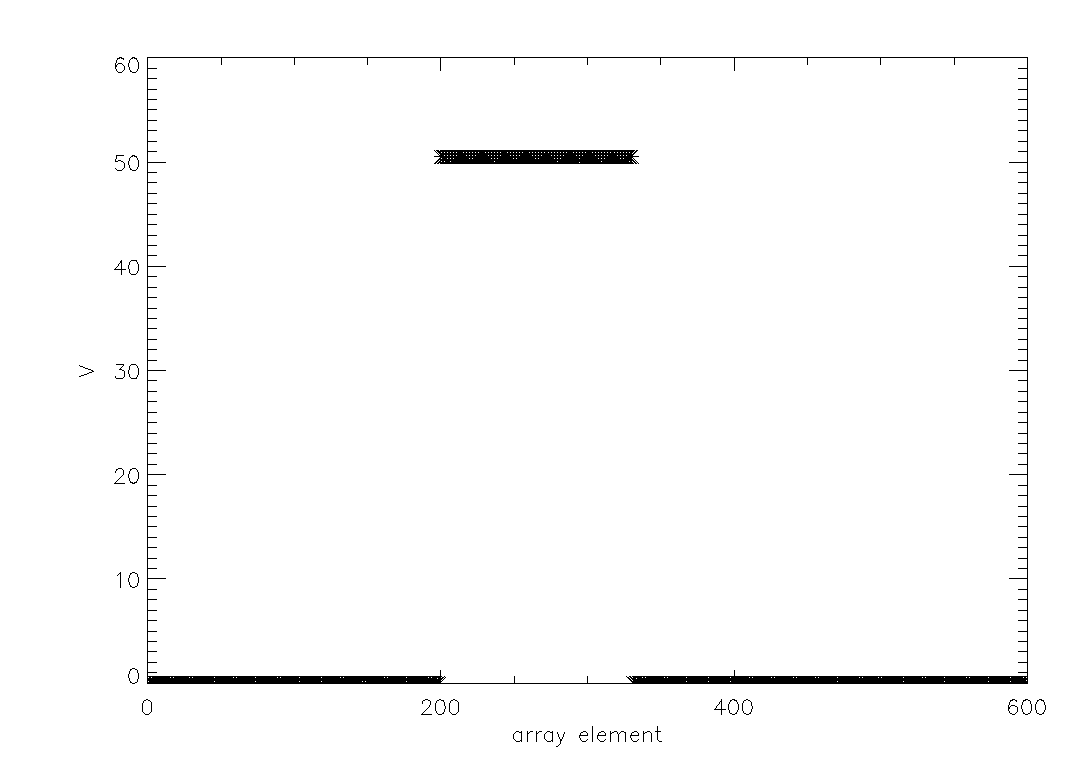
\includegraphics[width=0.49\columnwidth]{./full/test/V}
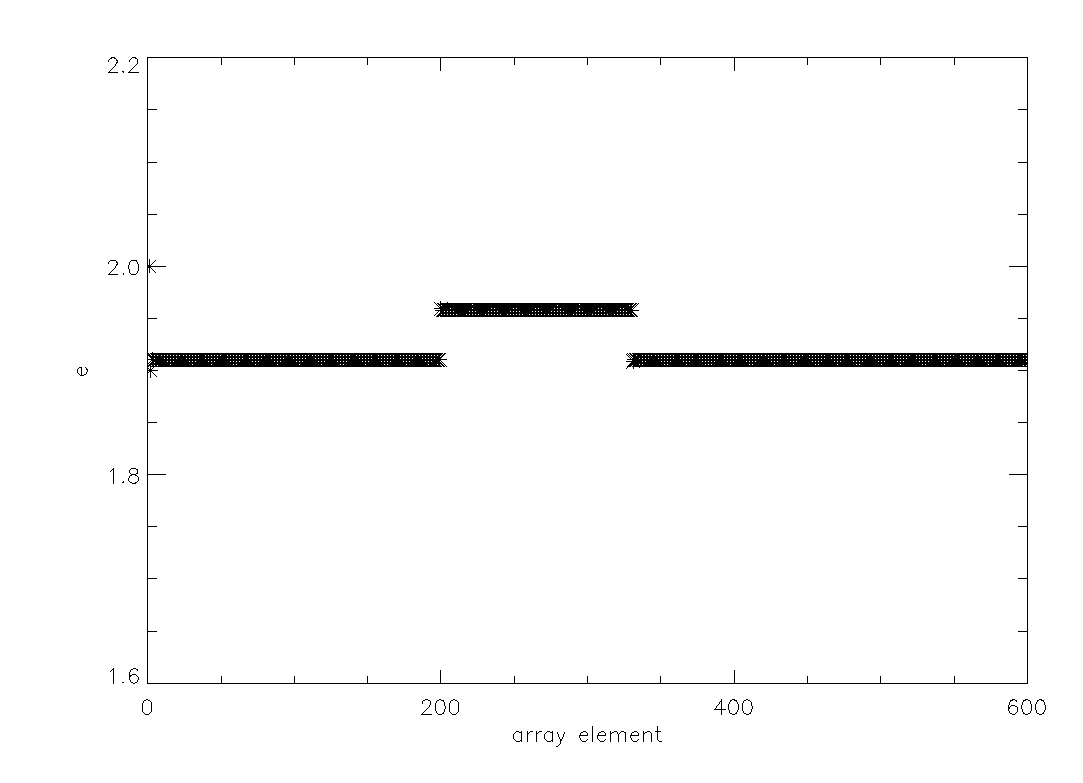
\includegraphics[width=0.49\columnwidth]{./full/test/e}
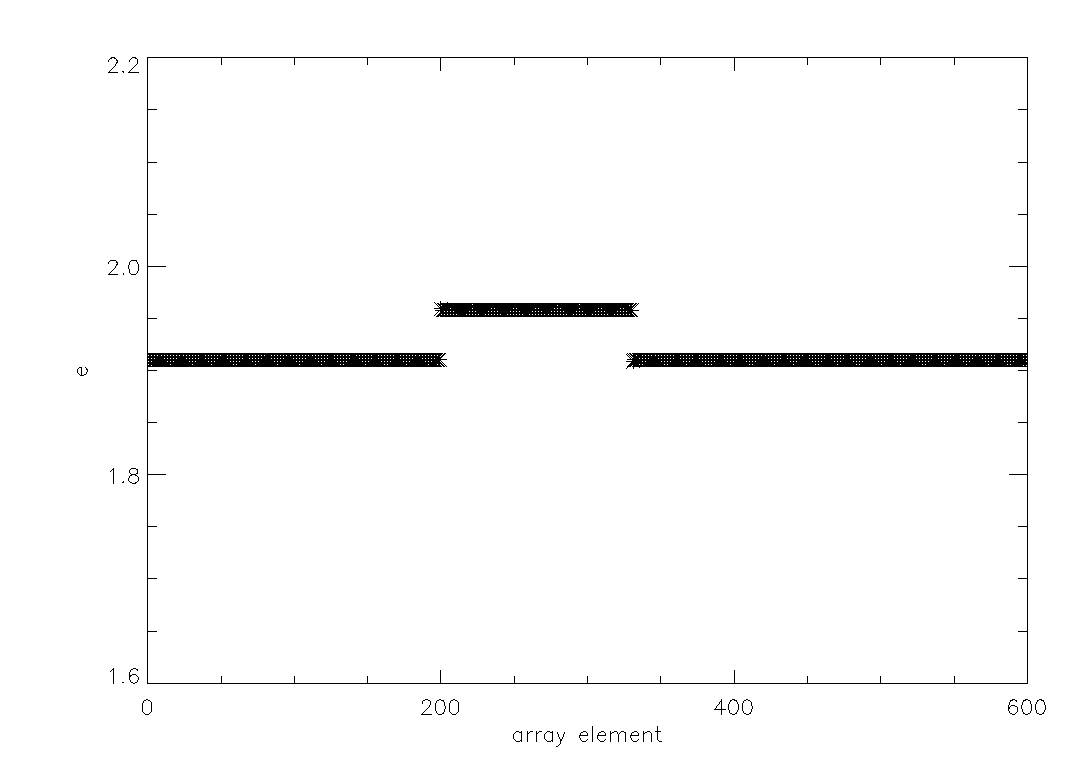
\includegraphics[width=0.49\columnwidth]{./full/test/e2}
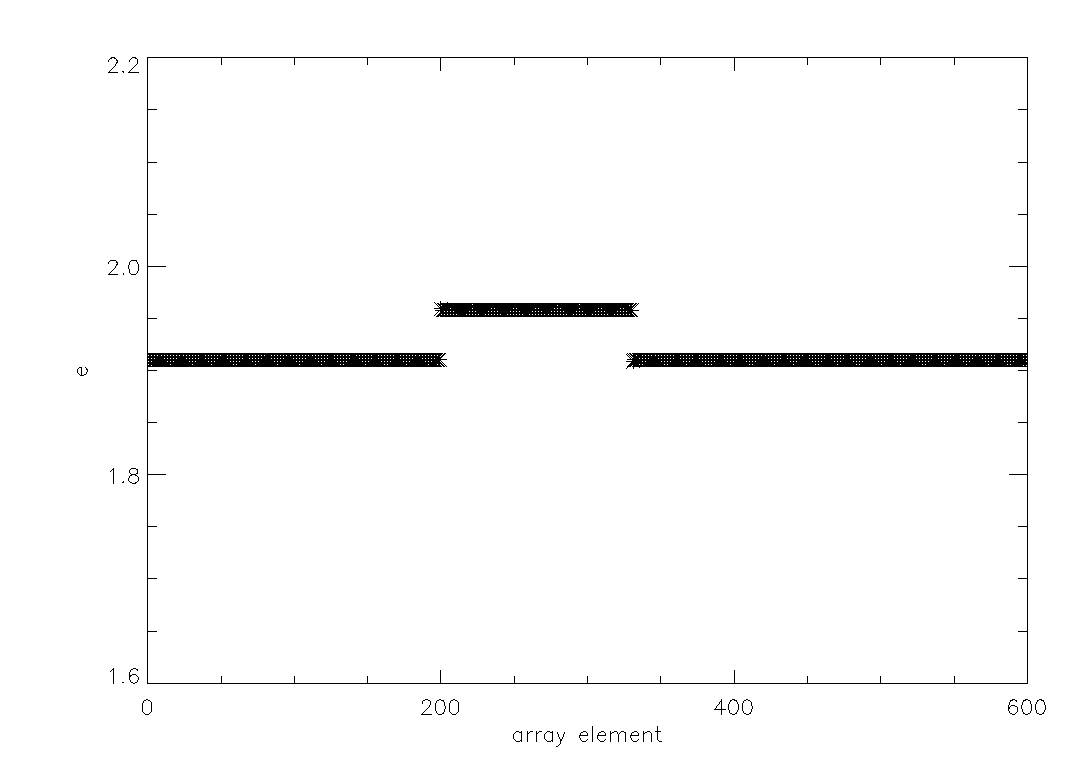
\includegraphics[width=0.49\columnwidth]{./full/test/e3}

   \end{center}
\caption{The plots here show recursion of the $e$ function over first, second and third iteration (top-right, bottom-left, bottom-right). The top-left graph is potential $V$ and is here to show the resemblance between its shape and that of $e$. On the first $e$ iteration we note that there is a `blip' (the start of the recursion relation). The last graph (bottom-right) is a third iteration and shows the same result as the second iteration. Number of gridpoints: $N_g= 600$.}
\label{fig.test_e}
\end{figure}

As corroborative evidence I present the outputs from a 3D simulation; figure \ref{fig.test_bound} shows a 2D slice where the wave-packet (shown as $\psi^*\psi$) passes through all 4 boundaries in the plane. There is no underlying potential well so the wave-packet behaved as a free particle and shows dispersion over time.

\begin{figure}[htb]
   \begin{center}
     %\leavevmode
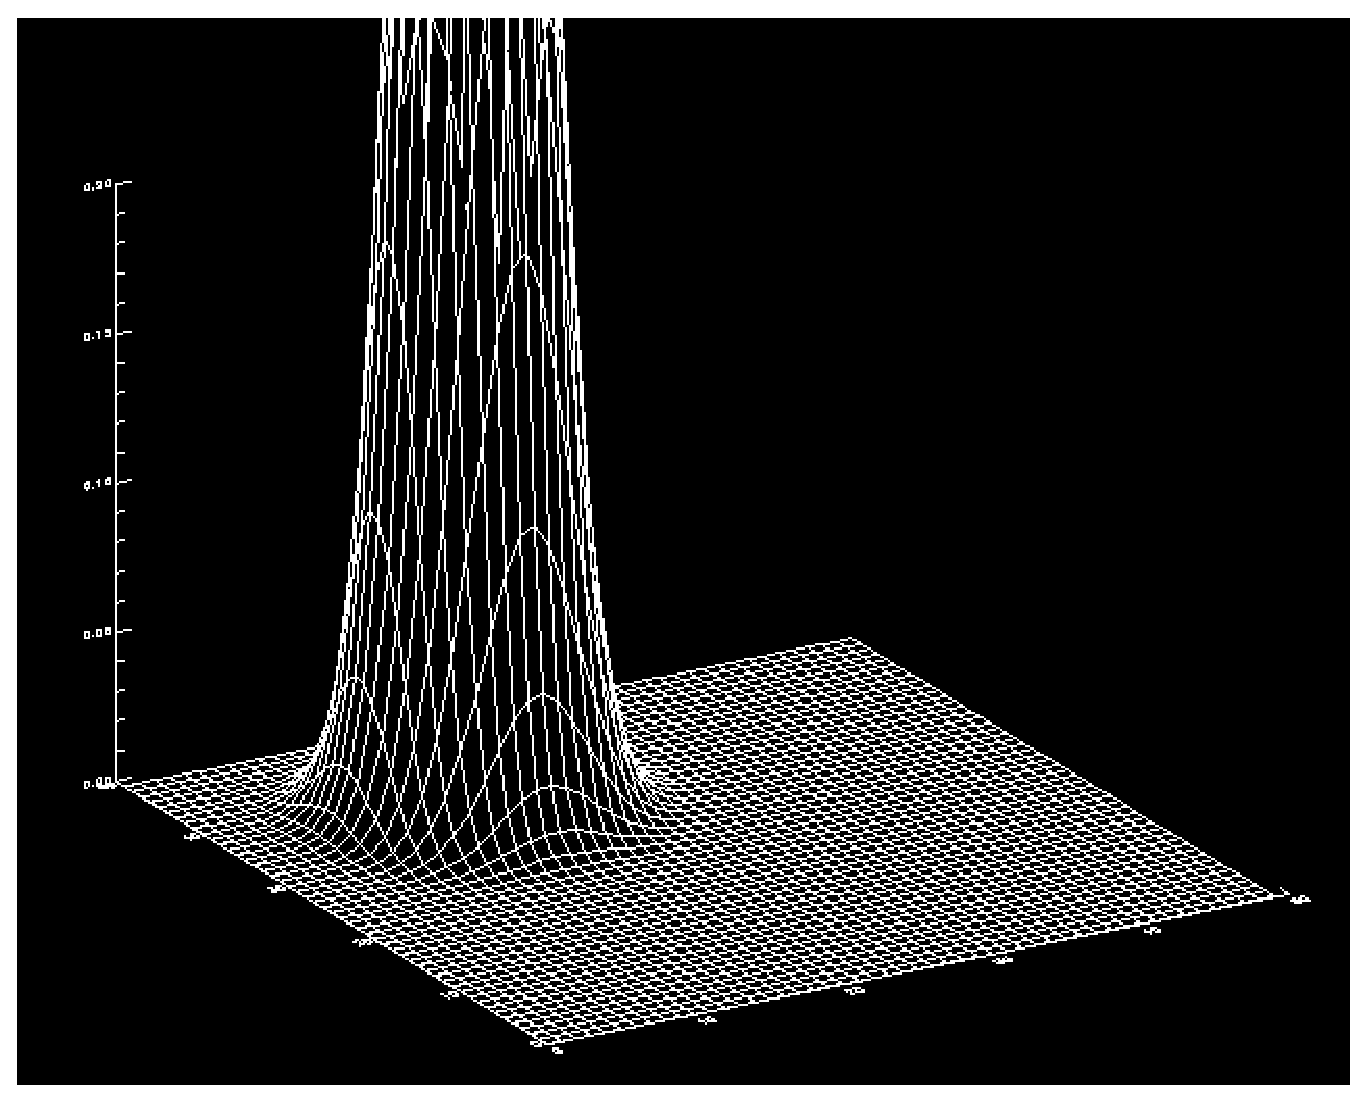
\includegraphics[width=0.49\columnwidth]{./full/test/deltas_00}
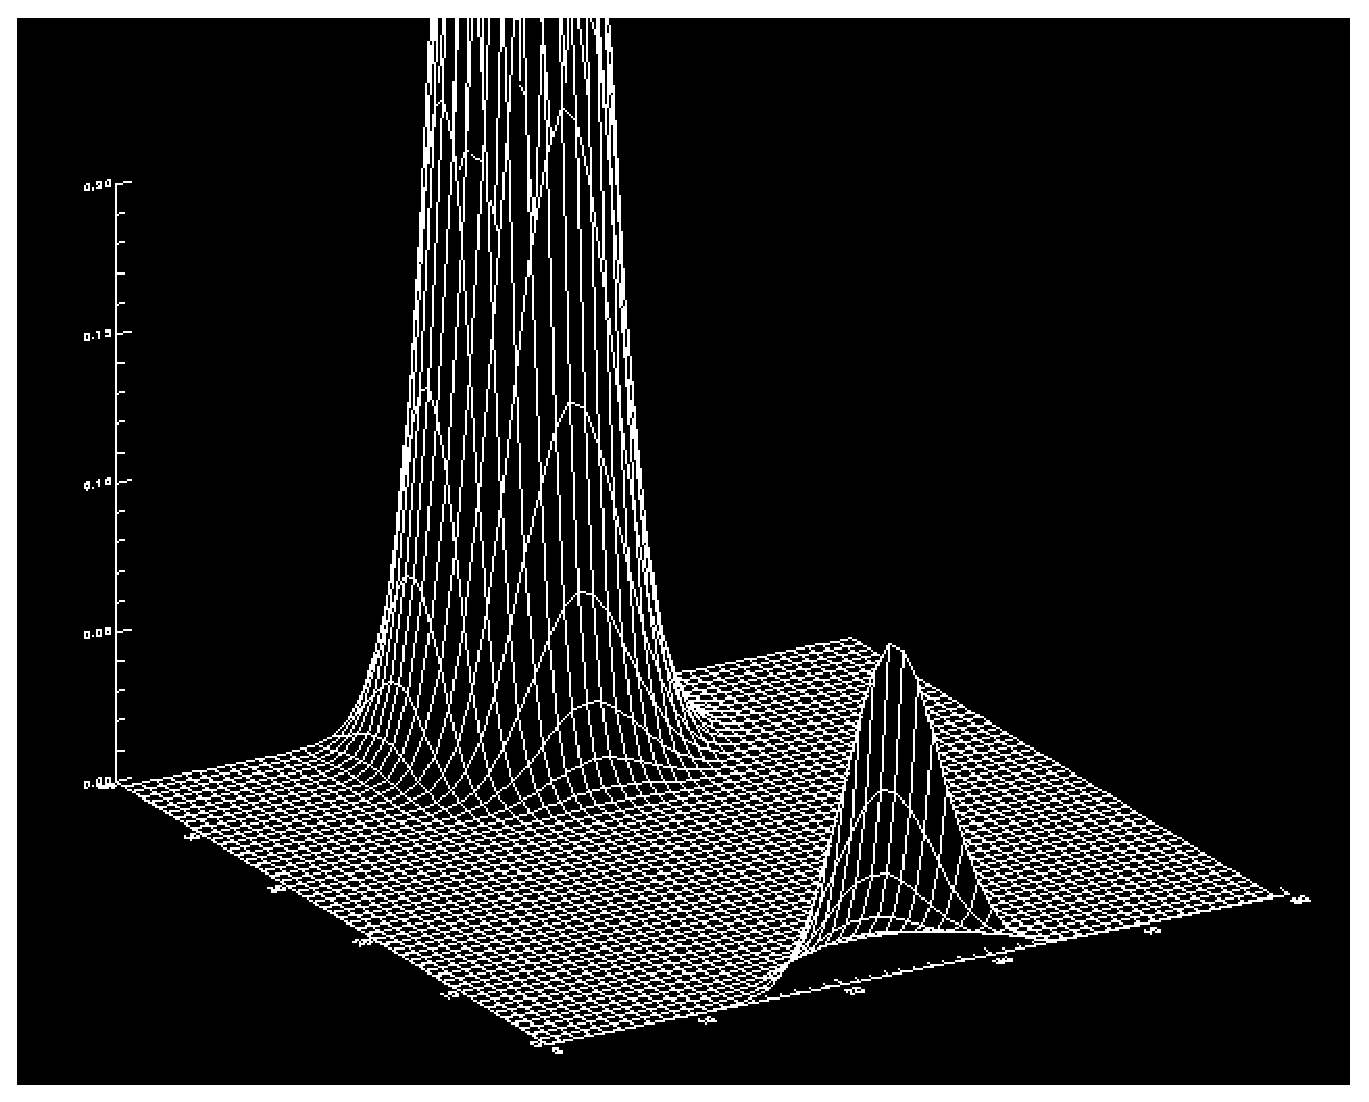
\includegraphics[width=0.49\columnwidth]{./full/test/deltas_10}
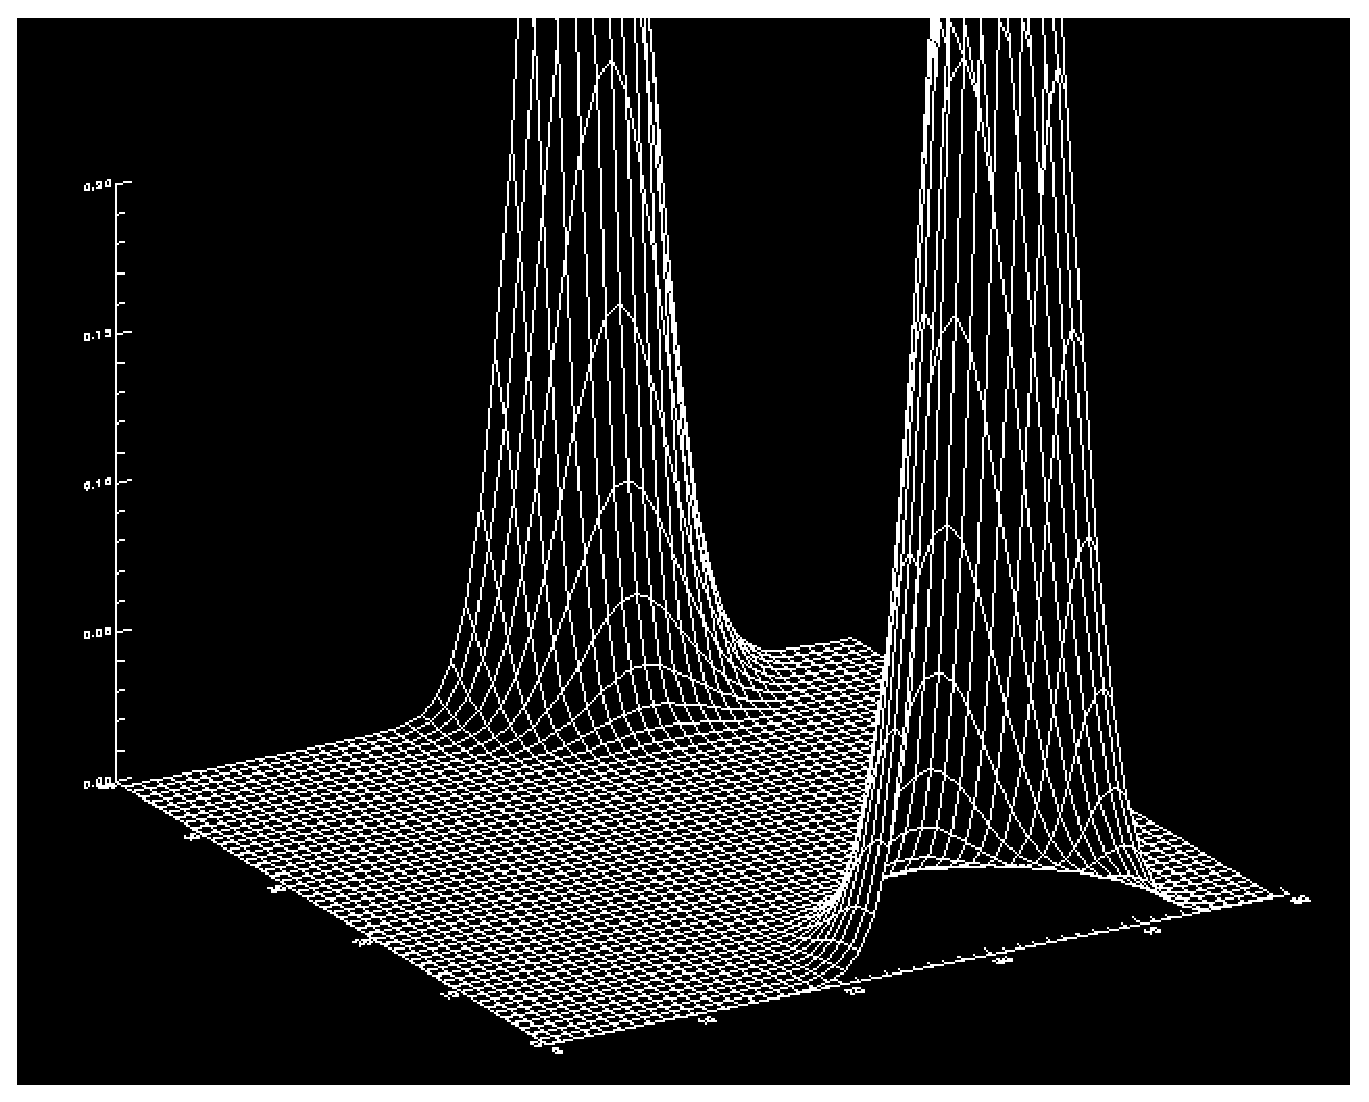
\includegraphics[width=0.49\columnwidth]{./full/test/deltas_20}
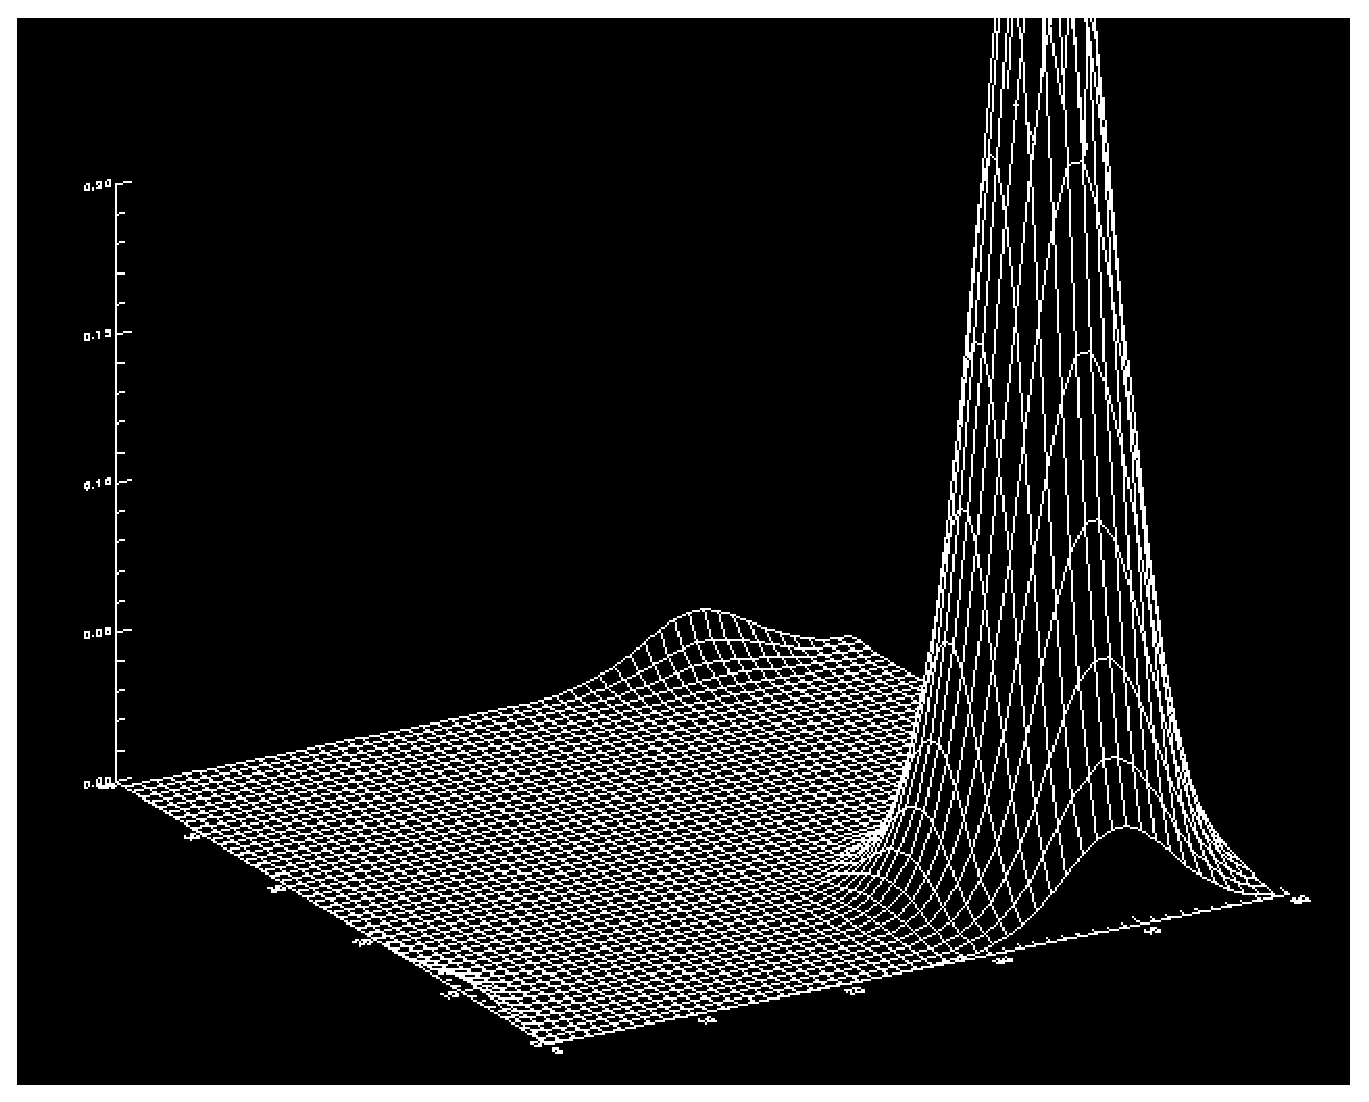
\includegraphics[width=0.49\columnwidth]{./full/test/deltas_30}
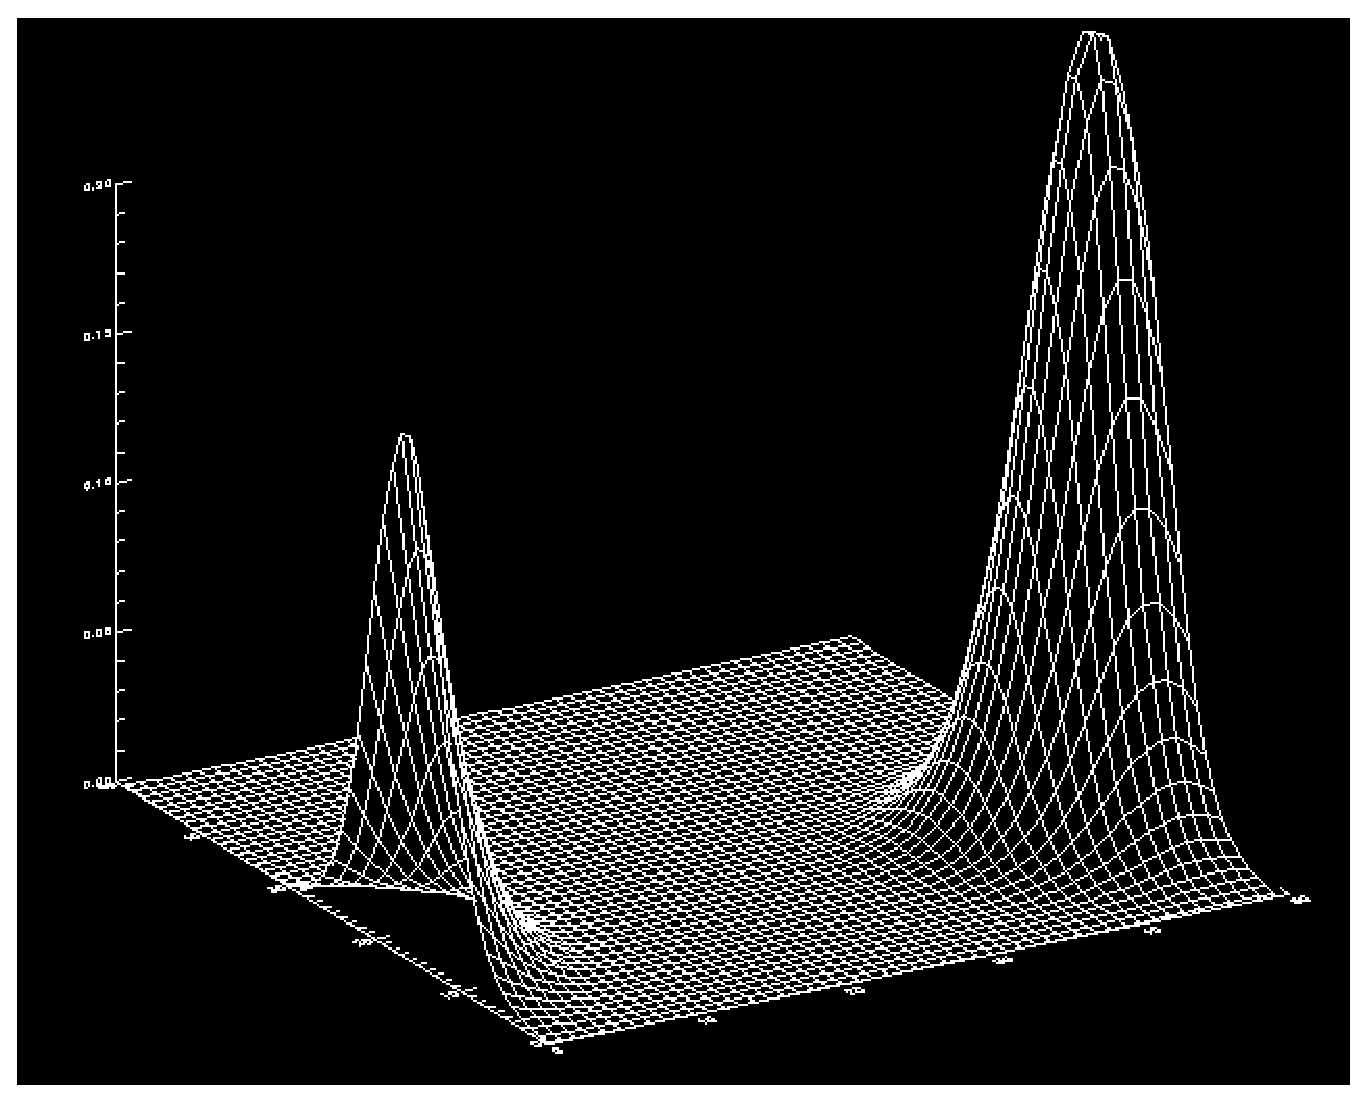
\includegraphics[width=0.49\columnwidth]{./full/test/deltas_40}
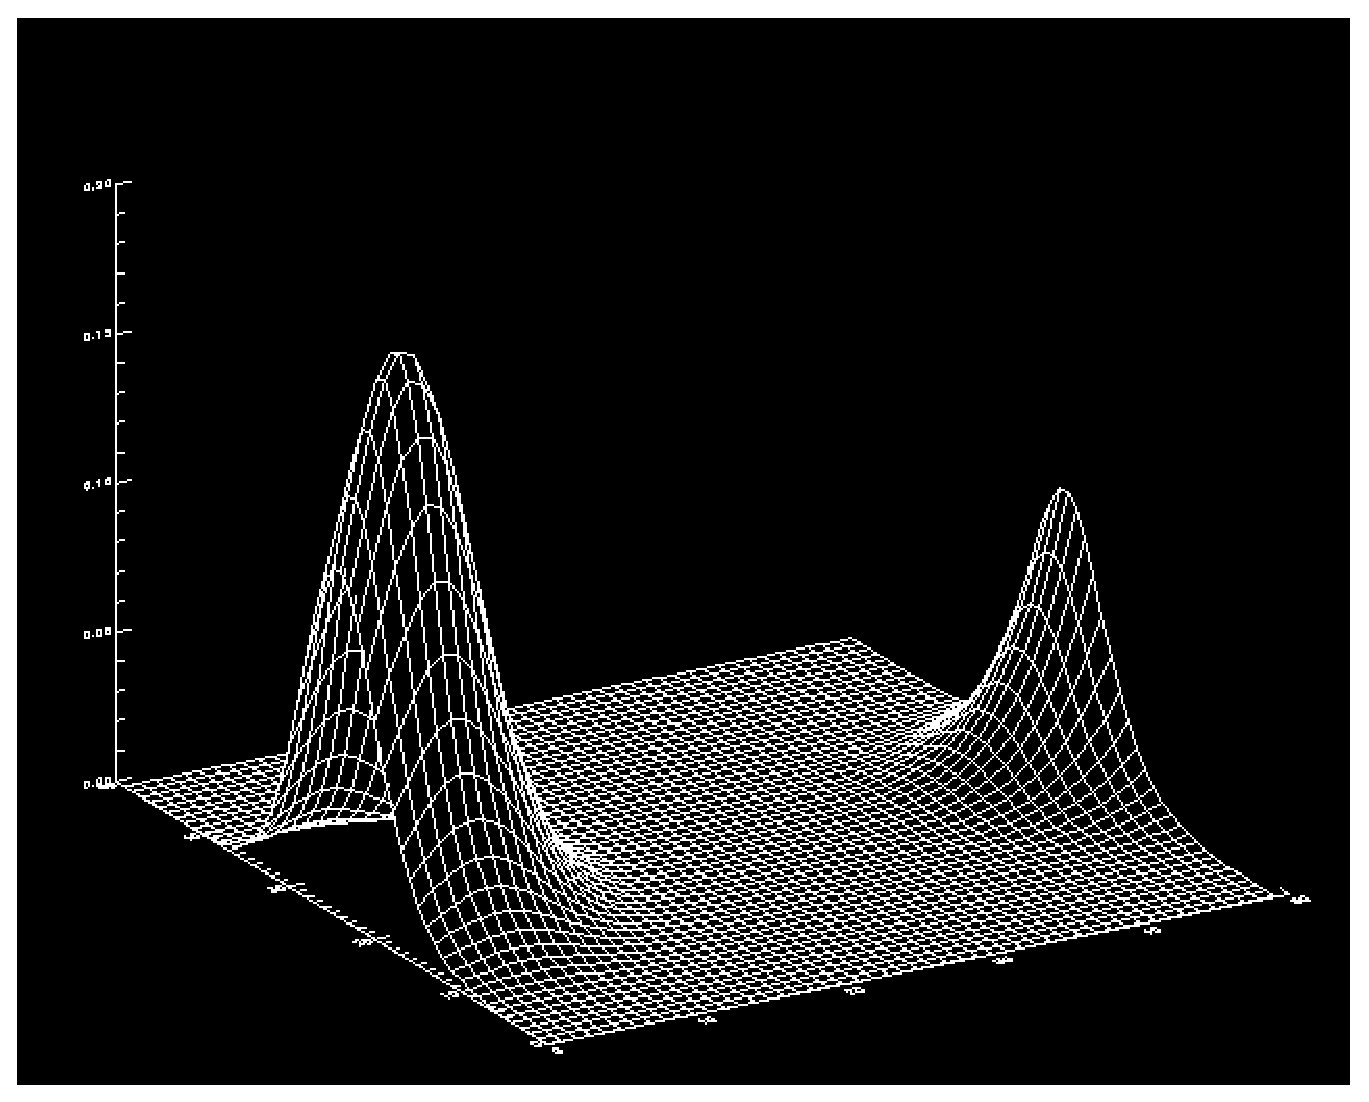
\includegraphics[width=0.49\columnwidth]{./full/test/deltas_50}
   \end{center}
\caption{The plots here show a wave-packet (or the `envelope of the wavefunction', which is the density $\psi^*\psi$) passing through all four boundaries of a 2D plane, the results were generated from a 3D code.}
\label{fig.test_bound}
\end{figure}

In testing, we explored what would happen to a wavefunction near the boundary when using a simple Goldberg algorithm -- that is, without the re-iteration of the auxiliary functions $e$ and $f$. As the edges of the system are not defined then the wavefunction appears to hit a hidden boundary. This effect was seen as a type of feedback (the wavefunction spikes up as if compressed by a potential barrier). This also resulted in a loss of mass at the boundaries whenever the wavefunction `escapes' out of the system. The feedback is obviously a numerical problem as the edge of the system should not be a barrier. With a smooth transition across the edge of the system then there should be no feedback.

An interesting result from running a wave-mechanics code is that of a stationary gaussian wave that is allowed to freely disperse without an underlying potential. If the code includes periodic boundaries then it is possible for the edges of the gaussian wavefunction to disperse across the boundary and eventually come back to interfere with itself.

The result is something that is akin to beat phenomena, where two frequencies compete with each other. The gaussian wavepacket is the envelope ($\psi \psi^*$) with a certain characteristic length but the wavefunction also has a (higher) carrier frequency. When the wave interferes with itself (or a neighbouring piece of the Universe, adopting the cosmology analogy where a simulation is quasi-infinite) under periodic boundaries the envelope acquires an additional frequency on top of the underlying gaussian envelope.

A brief look at this effect is presented in figure \ref{fig.interfere}. The results were generated using a 1D code that implements periodic boundary conditions, the outputs are at timesteps $0, 2000, 3000, 4000$. The effect of interference is minorly apparent in the second-last output but becomes a dominant feature in the last output where it is assumed that the wavefunction has passed through the boundary on both sides wrapped back in upon itself.

\begin{figure}[htb]
   \begin{center}
     %\leavevmode

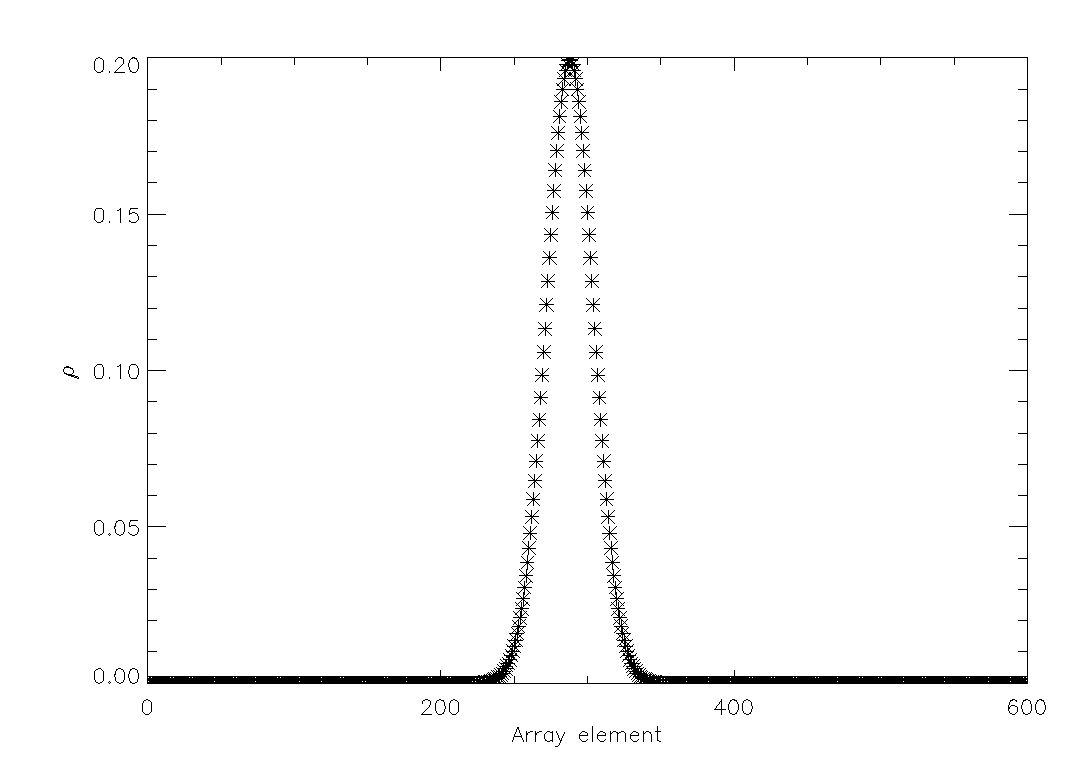
\includegraphics[width=0.49\columnwidth]{./full/periodic/rho.eps}
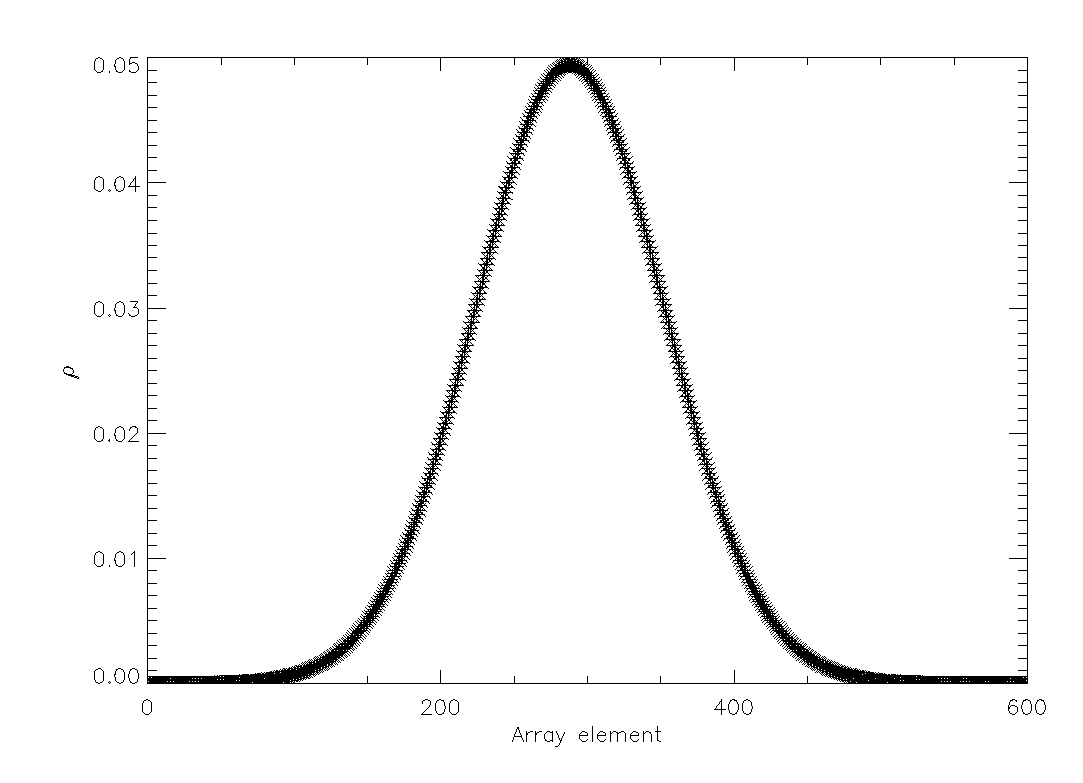
\includegraphics[width=0.49\columnwidth]{./full/periodic/rho_ev_2000.eps}
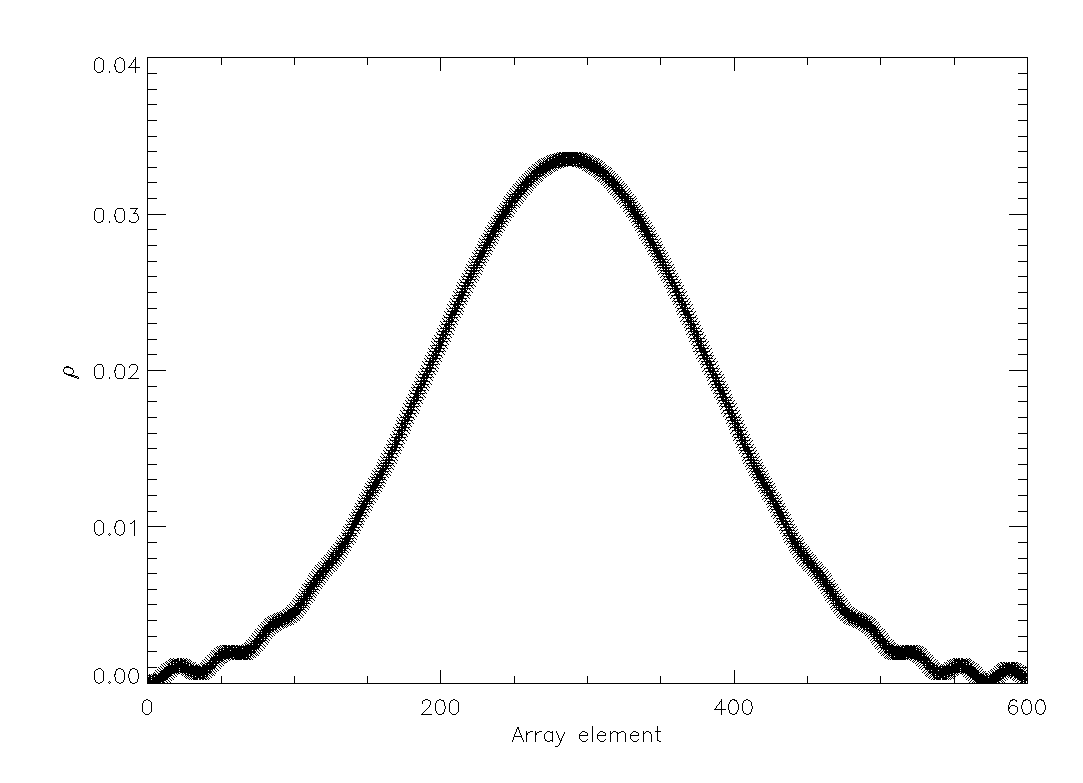
\includegraphics[width=0.49\columnwidth]{./full/periodic/rho_ev_3000.eps}
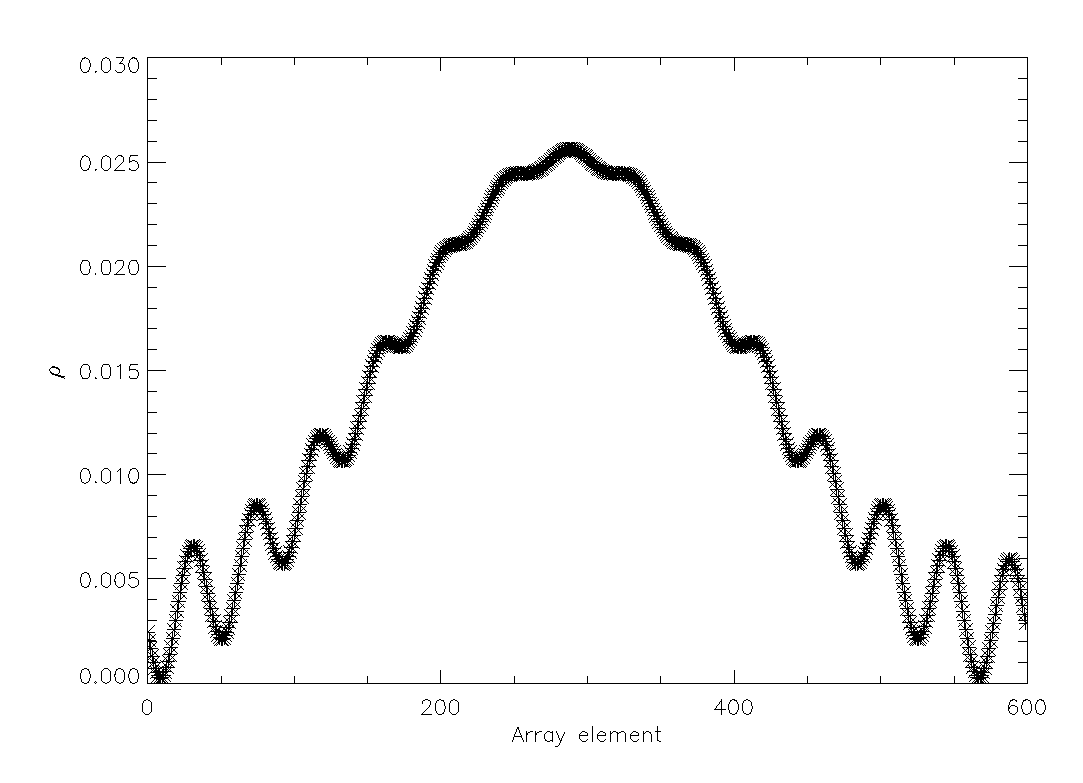
\includegraphics[width=0.49\columnwidth]{./full/periodic/rho_ev_4000.eps}

   \end{center}
\caption{The outputs at timesteps of $t = 0, 2000, 3000, 4000$. The initial gaussian wave-packet $\psi^*\psi$ is thin and centred within the box. Periodic boundaries were implemented. The wave-packet disperses and self-interferes once the wavefunction has crossed significantly pass the boundary.}
\label{fig.interfere}
\end{figure}

Such a result is important when considering the full cosmological simulations later. We need to ask ourselves what do we expect when the wavefunction crosses over the boundary and how far must it travel in order to create this (feedback) interference effect.

The results from the cosmological simulations in a later subsection (\ref{cos_sim}) have greater variation in the range of densities than first expected. In this later subsection I show a comparison with the `industry standard' code GADGET-2 which is providing our benchmark and hence provides what we expect from a cosmological code. The variation shown in the density outputs from wave-mechanics is far greater than that of GADGET-2. At first we considered that this variation was due to feedback this is now thought to be unlikely. From the wave-mechanics results it is clear that the waves (in general) have not crossed the entire length of the box, it even appears unlikely that any wave has travelled half of one box length.

In our study of feedback in this section the wavefunction must have dispersed a minimum of one box length and hence it gives a self-interaction pattern (shown in figure \ref{fig.interfere}). Here the wave-packet $\psi^*\psi$ (the density) has dispersed and is free of an internal or external potential. As is clear from the figure, the central density decreases in height as the width increases.

We performed several tests of the codes in all dimensions, with one of the tests being to see how fast a wavefunction will disperse. We found that the dispersion and subsequent feedback effect is dependent on the choice of $\nu$. Large values of $\nu$ will allow for faster dispersion and hence feedback will be seen earlier. However, such an effect requires the waves to pass far across each boundary which is further than should be typically allowed in a cosmological simulation. The typical $\nu$ values used in the cosmological simulations are quite small -- for example, $10^{-7}$; during our tests such a small value showed only a small degree of dispersion and hence the time required to see feedback is far longer than the simulation time.

We modified this test to include a second gaussian peak in the box. The peaks are situated in such a way that the system is symmetric about the midpoint of the $x$-axis. We performed three such tests and kept the initial conditions the same (except for an additional kinetic boost in the second test). In the first case we had no gravity; the second test involved an initial kick in velocity but no gravity while the third test had no initial kick in velocity but the peaks were subjected to gravitational interaction.

In the first test (see figure \ref{fig.twodisp}) we wished to see what happened when the two peaks are allowed to freely disperse with no initial kinetic energy and are not subject to the force of gravity. As expected the two peaks disperse and eventually overlap each other. The pattern of the overlap is what we expect from a wave-mechanics code. We see interference effects when the wavefunctions over lap; ideally, we would not see this in a classical code which raises a point of contention when using a wave-mechanics code. Such effects should be minimized when simulating a classical system.


\begin{figure}[htb]
   \begin{center}
     %\leavevmode

\includegraphics[width=0.49\columnwidth]{./full/BB/delta.eps}

\includegraphics[width=0.49\columnwidth]{./full/BB/delta_ev60.eps}

\includegraphics[width=0.49\columnwidth]{./full/BB/delta_ev100.eps}

\includegraphics[width=0.49\columnwidth]{./full/BB/delta_ev120.eps}

\includegraphics[width=0.49\columnwidth]{./full/BB/delta_ev140.eps}

\includegraphics[width=0.49\columnwidth]{./full/BB/delta_ev180.eps}

   \end{center}
\caption{This figure shows the dispersion of gaussian peaks in a box.  The output times are at timesteps of $0, 60, 100, 120, 140, 180$.}
\label{fig.twodisp}
\end{figure}

Another test of our code is to provide two gaussian peaks with some initial kinetic energy, rather than let them freely disperse. We also omitted gravity from this test. The results are shown in figure \ref{fig.twokin}; we plot normalized density, $\rho$, against a normalized length, $x$. This simulation used 512 grid elements. The two peaks have met by timestep 40 and are almost apart in the last plot at timestep 100. The speed of dispersion is set by the parameter $\nu = \hbar/m$.

\begin{figure}[htb]
   \begin{center}
     %\leavevmode

\includegraphics[width=0.49\columnwidth]{./full/CC/delta.eps}

\includegraphics[width=0.49\columnwidth]{./full/CC/delta_ev20.eps}

\includegraphics[width=0.49\columnwidth]{./full/CC/delta_ev40.eps}

\includegraphics[width=0.49\columnwidth]{./full/CC/delta_ev60.eps}

\includegraphics[width=0.49\columnwidth]{./full/CC/delta_ev80.eps}

\includegraphics[width=0.49\columnwidth]{./full/CC/delta_ev100.eps}

   \end{center}
\caption{In this figure two gaussian peaks with some initial kinetic energy pass through each other and their evolution is observed. The peaks move with a constant velocity. The outputs are at timesteps of $0, 20, 40, 60, 80, 100$.}
\label{fig.twokin}
\end{figure}

One of the most important tests in one dimension is that of two peaks passing through each other under the influence of gravity. In this test the peaks had no initial kinetic energy. The results of this test are shown in figure \ref{fig.twograv}. The peaks appear to move slowly at first then accelerate through each other; the initial timesteps show little happening as the attraction towards each other is slow. The maximum peak achieved is when the two peaks fully meet in the middle (shown at timestep 160) but soon appear as two separate peaks not long after (timestep 200).

One of the most interesting features of this third test is that gravity appears to suppress the interference effects observed in the previous two tests. It does not, however, appear to be completely free of interference effects. This is expected as the two peaks are actually part of the same wavefunction, that is to say that they are coherent. This also explains why interference effects are seen in the previous tests. Such interference patterns, as mentioned, as not classical in nature hence should not be present in the simulation of a classical system.

\begin{figure}[htb]
   \begin{center}
     %\leavevmode

\includegraphics[width=0.49\columnwidth]{./full/AA/delta.eps}
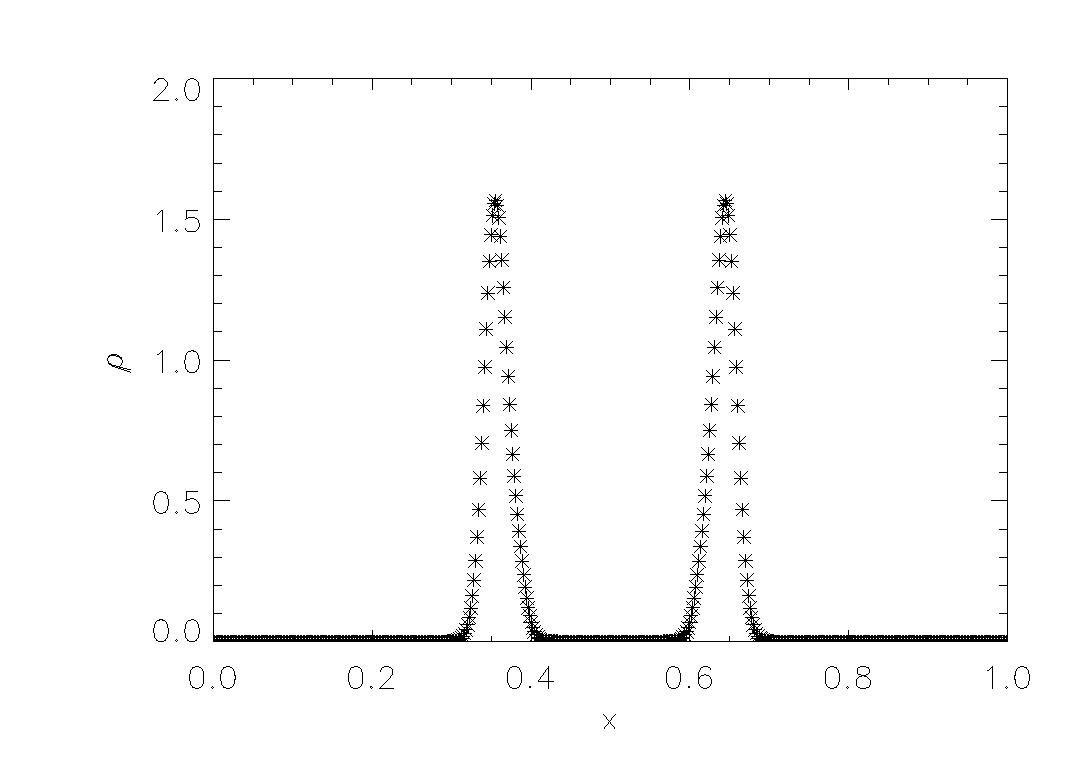
\includegraphics[width=0.49\columnwidth]{./full/AA/delta_ev40.eps}
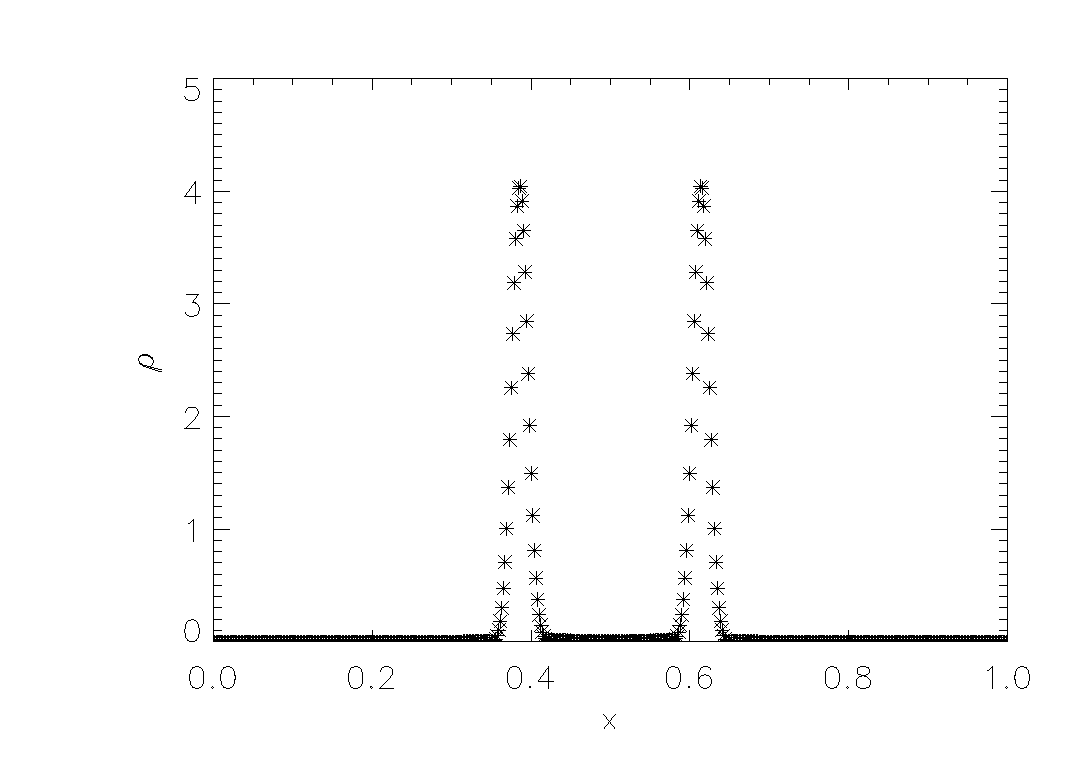
\includegraphics[width=0.49\columnwidth]{./full/AA/delta_ev80.eps}
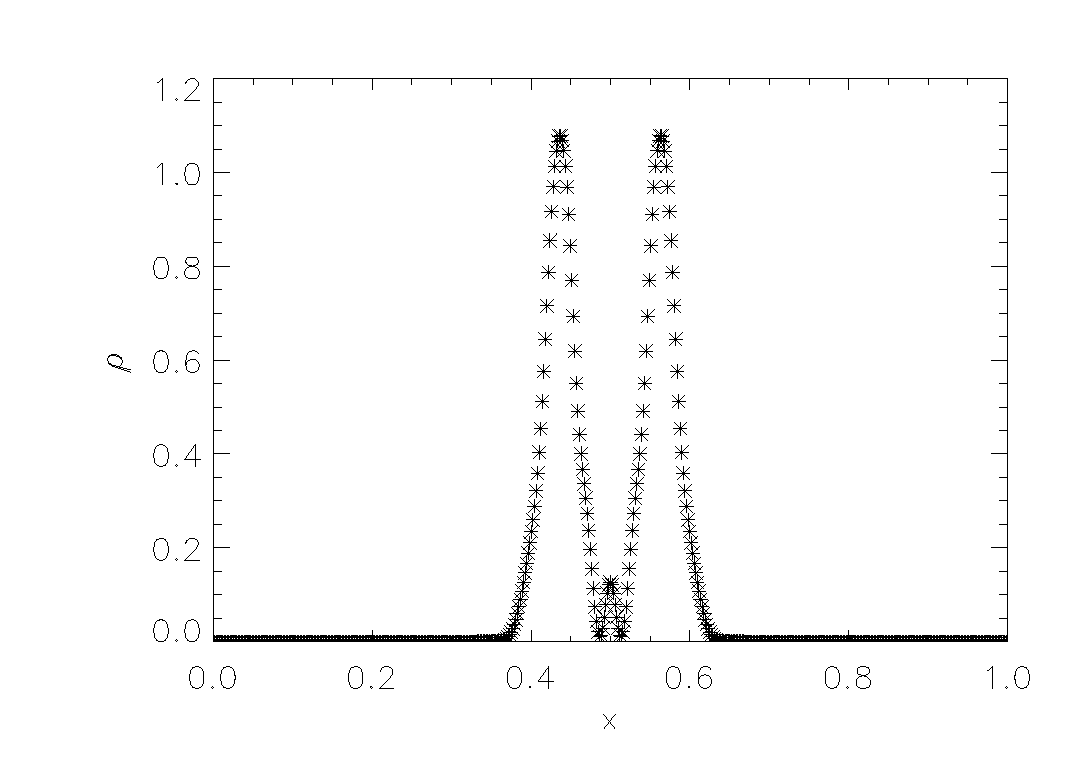
\includegraphics[width=0.49\columnwidth]{./full/AA/delta_ev120.eps}
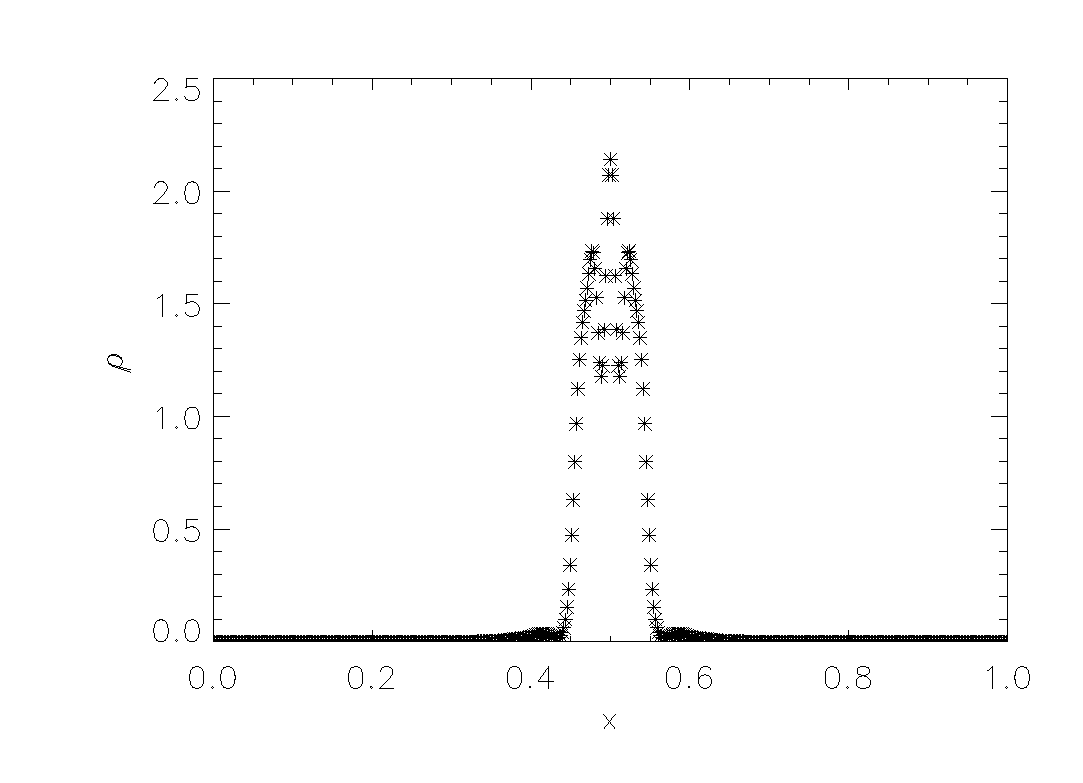
\includegraphics[width=0.49\columnwidth]{./full/AA/delta_ev160.eps}
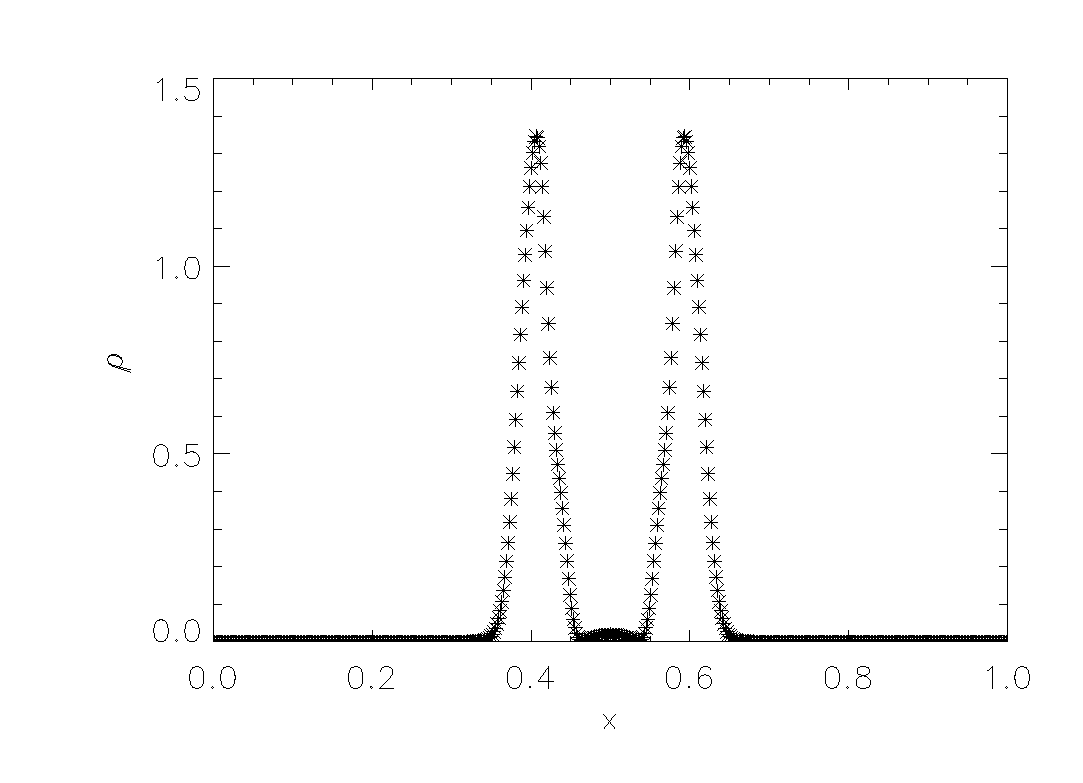
\includegraphics[width=0.49\columnwidth]{./full/AA/delta_ev200.eps}

   \end{center}
\caption{This figure shows the evolution of two gaussian peaks under the influence of gravity. The peaks move slowly at first as they attracted towards each other. The peaks speed up as they meet in the middle of the box and eventually pass through each other. The output times are at timesteps of $0, 40, 80, 120, 160, 200$.}
\label{fig.twograv}
\end{figure}


\subsection{2D Two-body gravitational interaction}
\label{twobody}
The first test of gravity in the 3D wave-mechanics code was that of a two-body gravitational interaction. In a traditional $N$-body code this test would involve two point particles interacting under the force of gravity (note: it is possible to give these particles an effect length via the softening length as mentioned in Chapter \ref{ch_2}). In wave-mechanics the particles are replaced by two gaussian wave-packets. As these two wave-packets are no longer point-like then there is no concern about two-body relaxation -- a problem that was highlighted earlier in section \ref{sec.dir_nb}.

The outputs of this test are shown in the series of plots \ref{fig.twobody}, \ref{fig.twobody2}, \ref{fig.twobody3}. The full test shows the two gaussians being attracted towards one another (during timesteps, t = [0, 30]). As the two peaks move towards each other they are observed to squeeze themselves under gravity: the peaks to become taller and thinner (as seen in the plot for time 10). Interestingly, they appear to relax and then repeat the process as they move towards the system's centre of mass where the two peaks pass through one another.

The next series of plots (\ref{fig.twobody2}) shows the two peaks passing through each other. At the mid-point when the peaks overlap they display a spiky pattern akin to the interference pattern of the double slit experiment (during timesteps, t = [35, 50]). After the pass through the two peaks move apart and journey to the starting point of the opposite peak. In the plot for timestep 65 we can see that some of the mass has been left in the middle after the interaction, this eventually disappears before the next collapse but it indicates that the masses have already passed through each other. This could be a potential way of tracing astrophysical objects that resemble this simple toy model (perhaps the Bullet Cluster -- where two distinct distributions of mass have passed through one another). A residual mass should follow the interaction but eventually this mass could be attracted towards their parent peaks.

By timestep 100 we can see that the two peaks have hit their turn-around radius. The residual mass has disappeared however the two peaks sit at these positions and re-arrange themselves under internal gravitational and presumably tidal forces. Then they begin their collapse again and are attracted towards each other. This time appears to be slightly different that the first pass through, as seen in the plot of timestep 125, there is a build up of mass at the centre before the two main peaks have interacted. By timestep 140 we can see the two peaks are starting to overlap and then have passed through each other by timestep 150.

\begin{figure}[htb]
   \begin{center}
     %\leavevmode
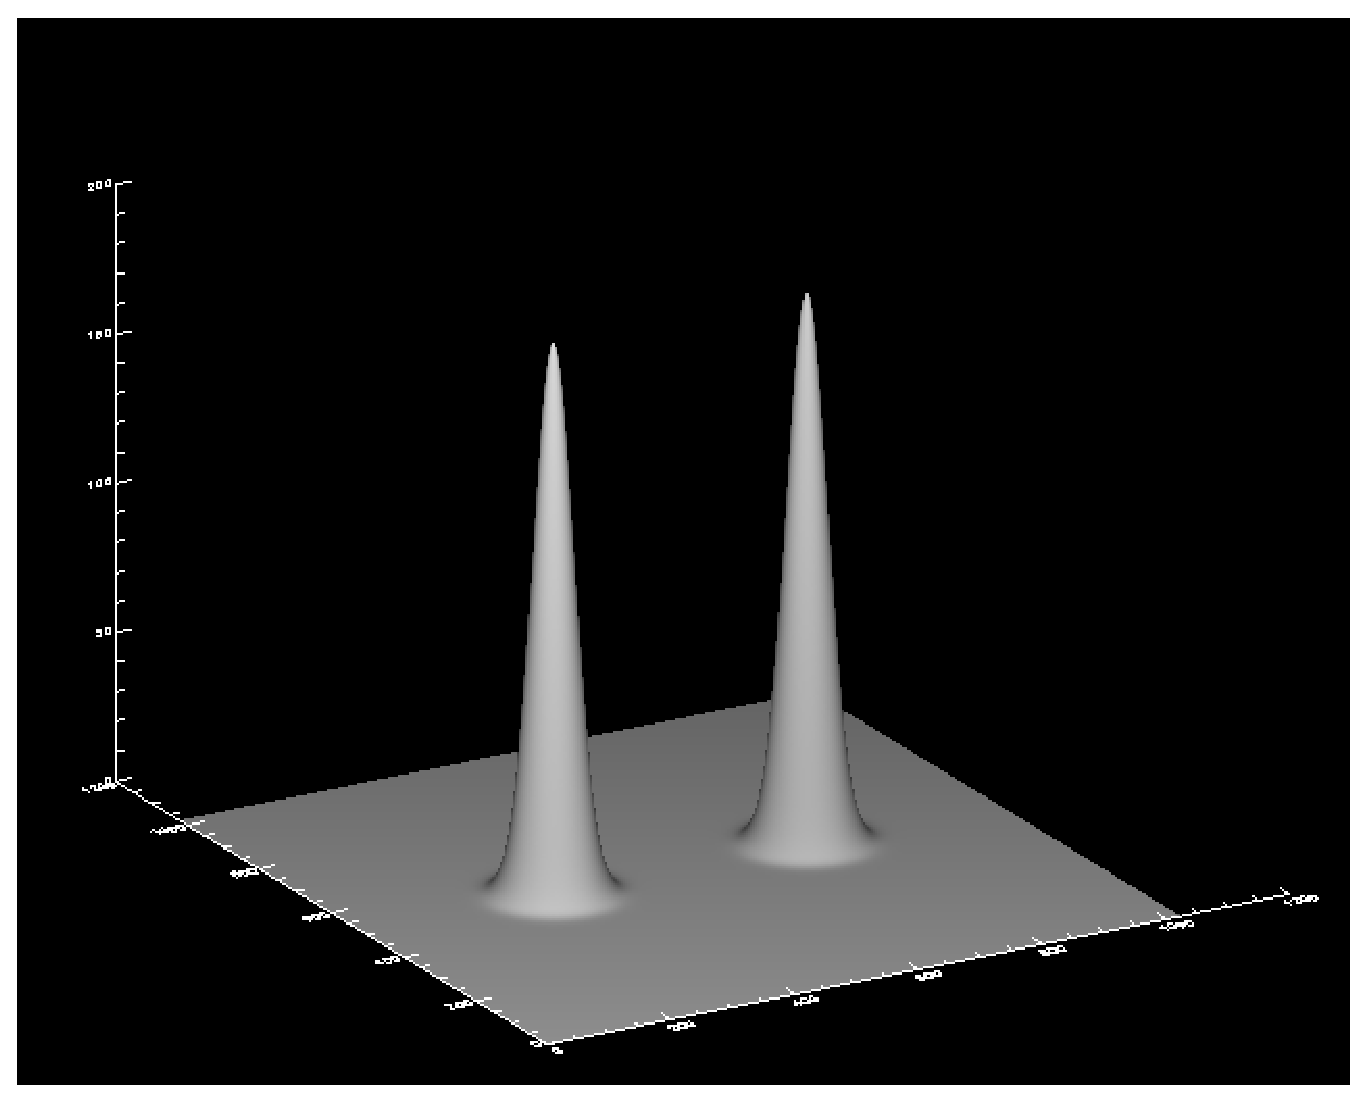
\includegraphics[width=0.49\columnwidth]{./full/twobody/deltas_000}
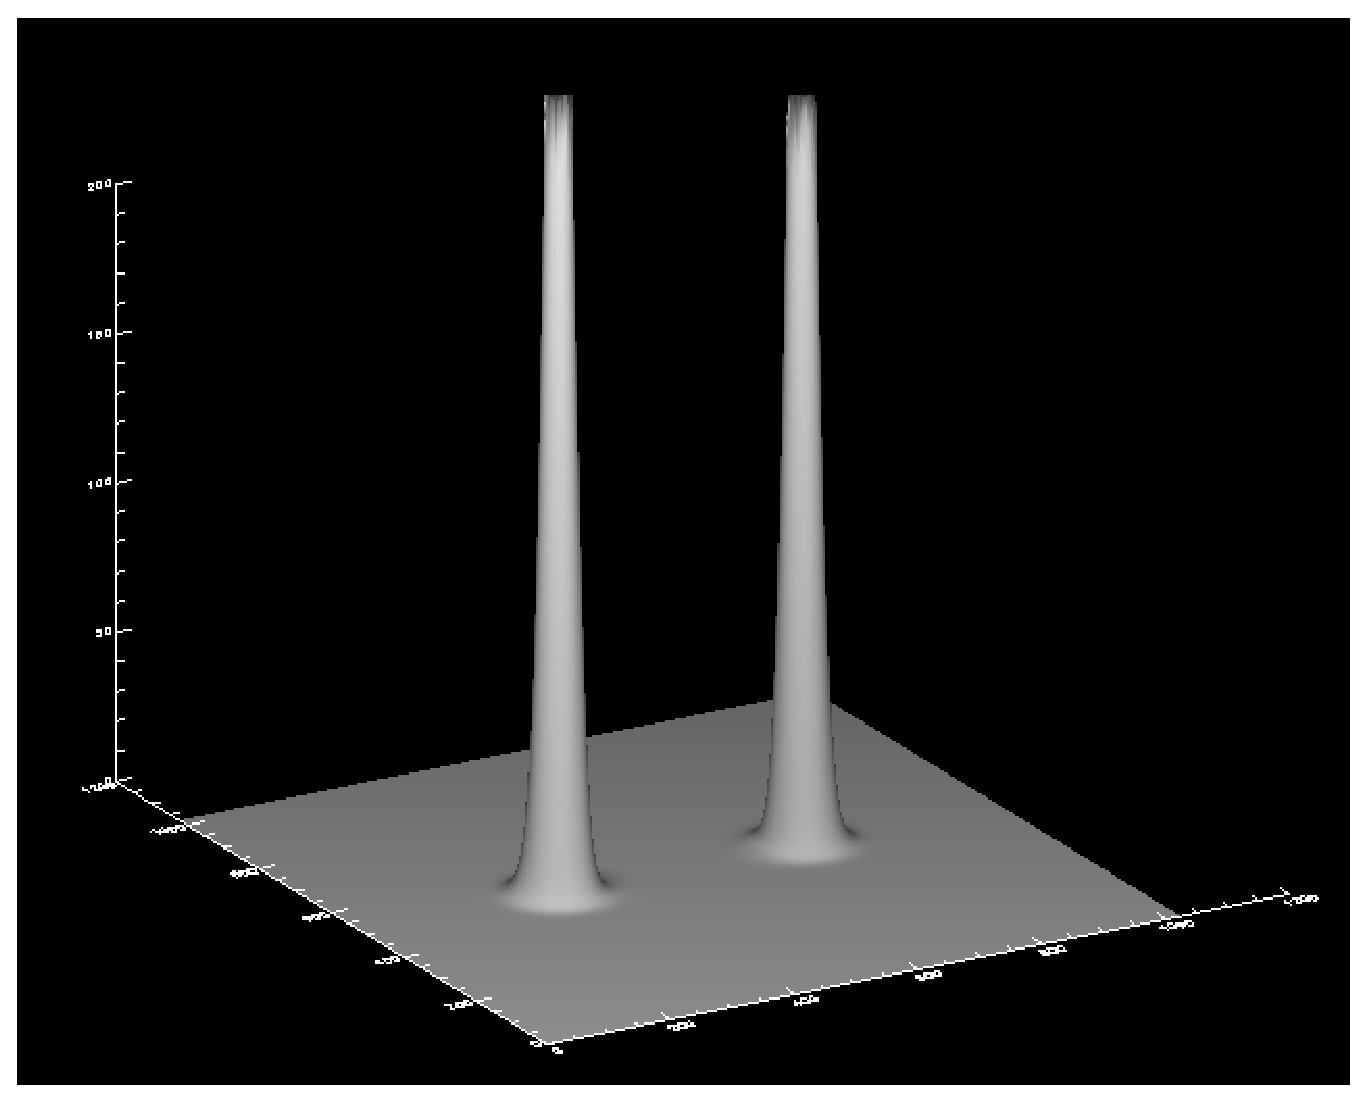
\includegraphics[width=0.49\columnwidth]{./full/twobody/deltas_010}
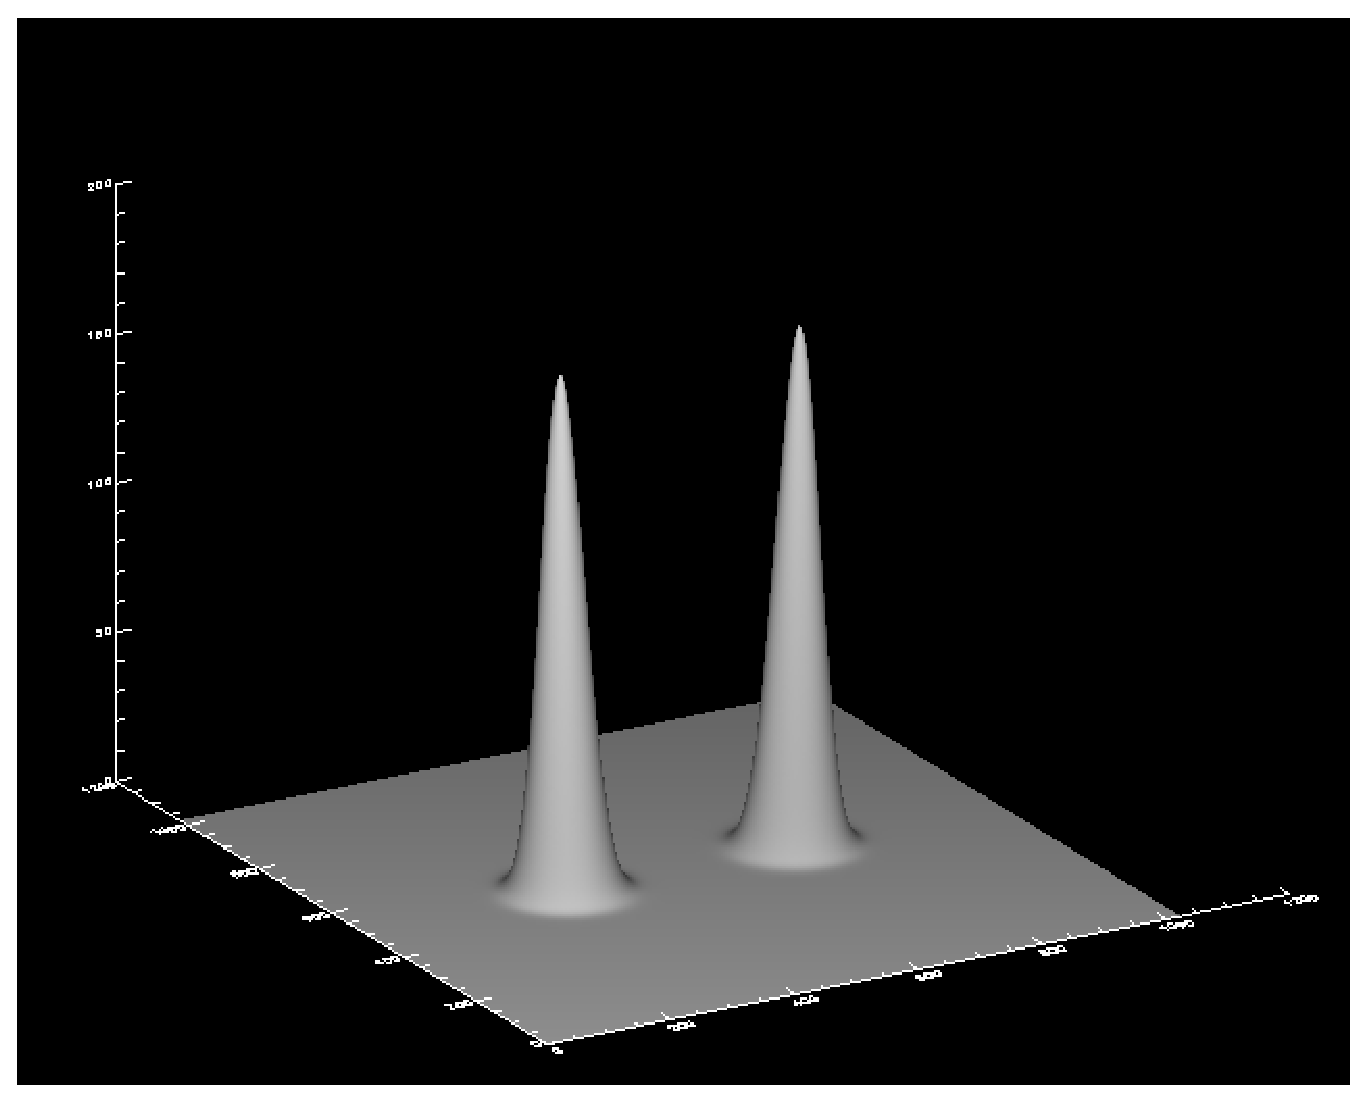
\includegraphics[width=0.49\columnwidth]{./full/twobody/deltas_015}
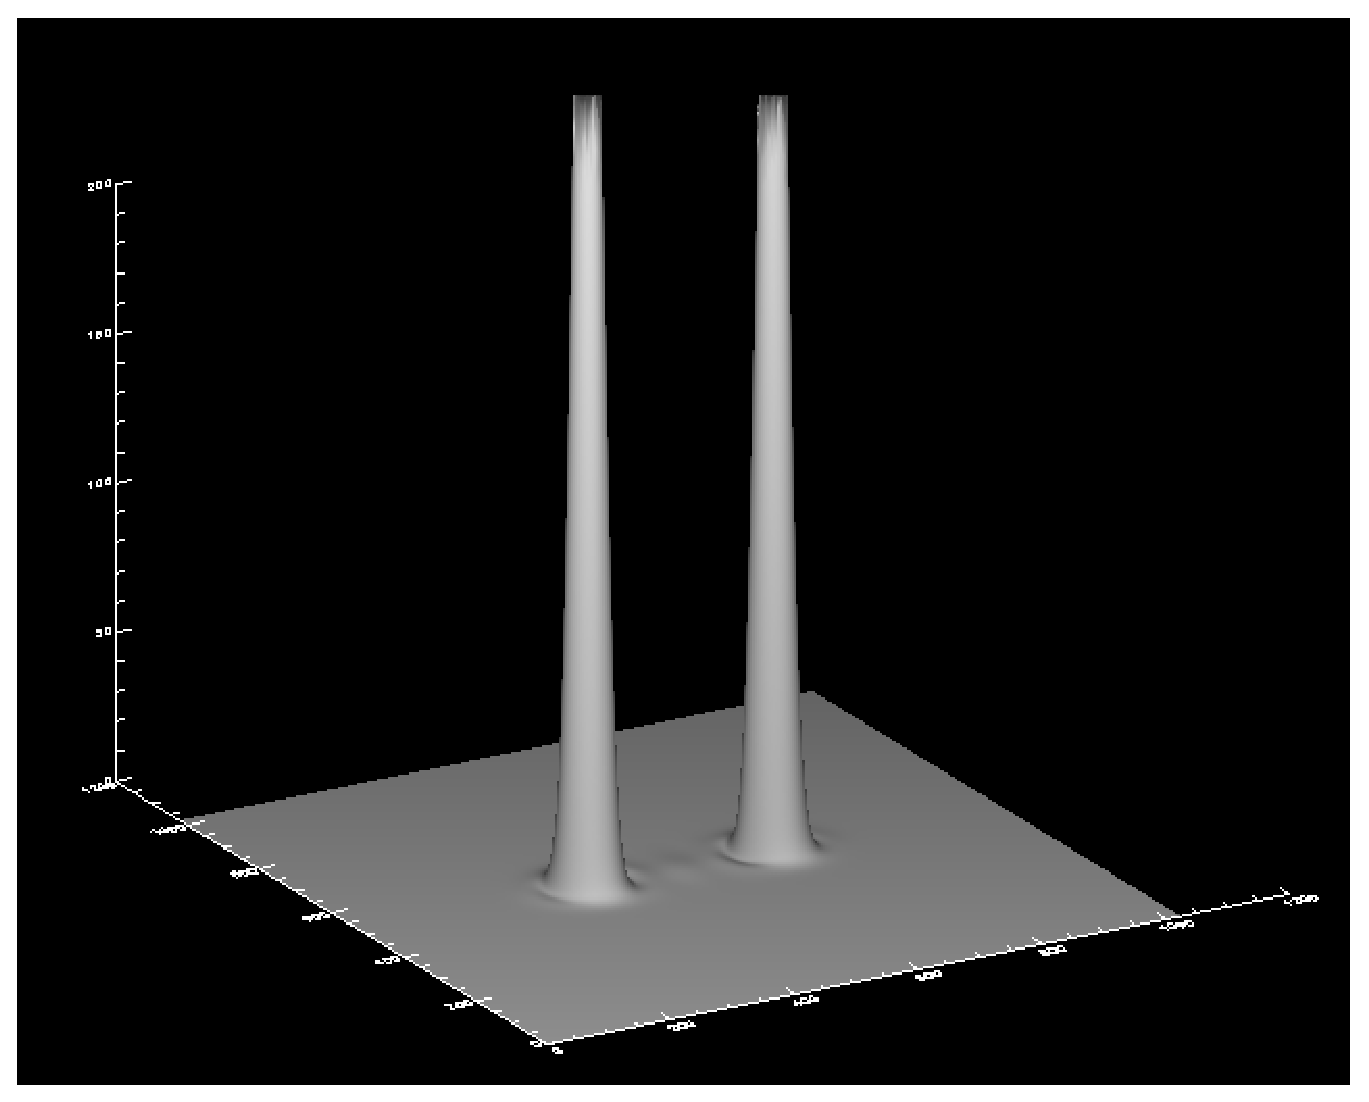
\includegraphics[width=0.49\columnwidth]{./full/twobody/deltas_025}
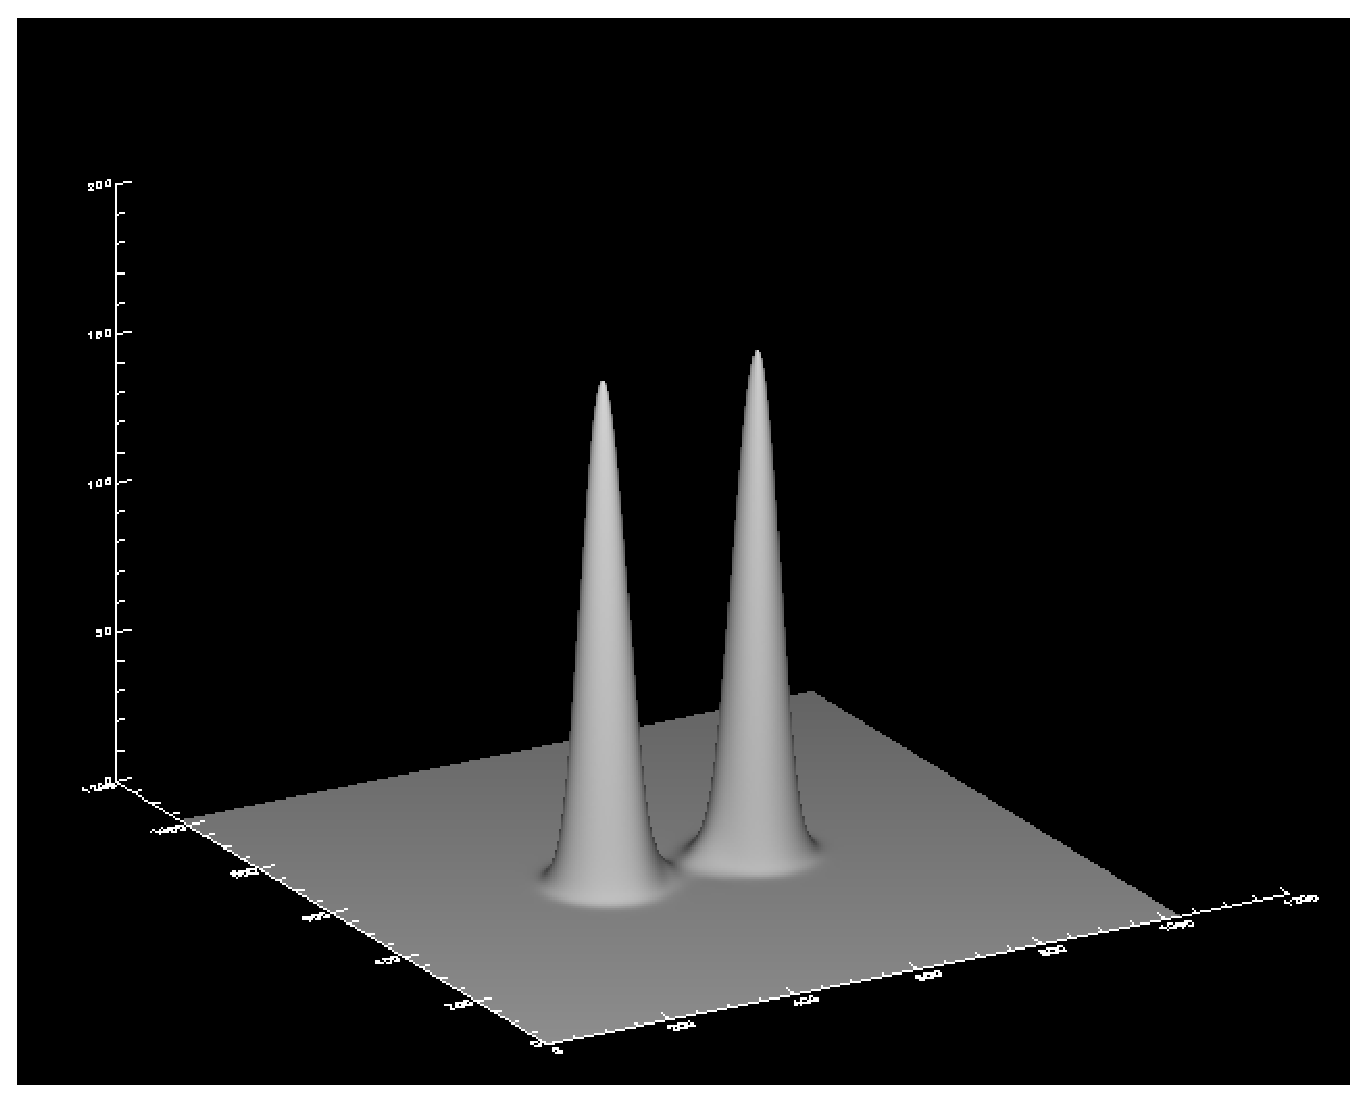
\includegraphics[width=0.49\columnwidth]{./full/twobody/deltas_030}
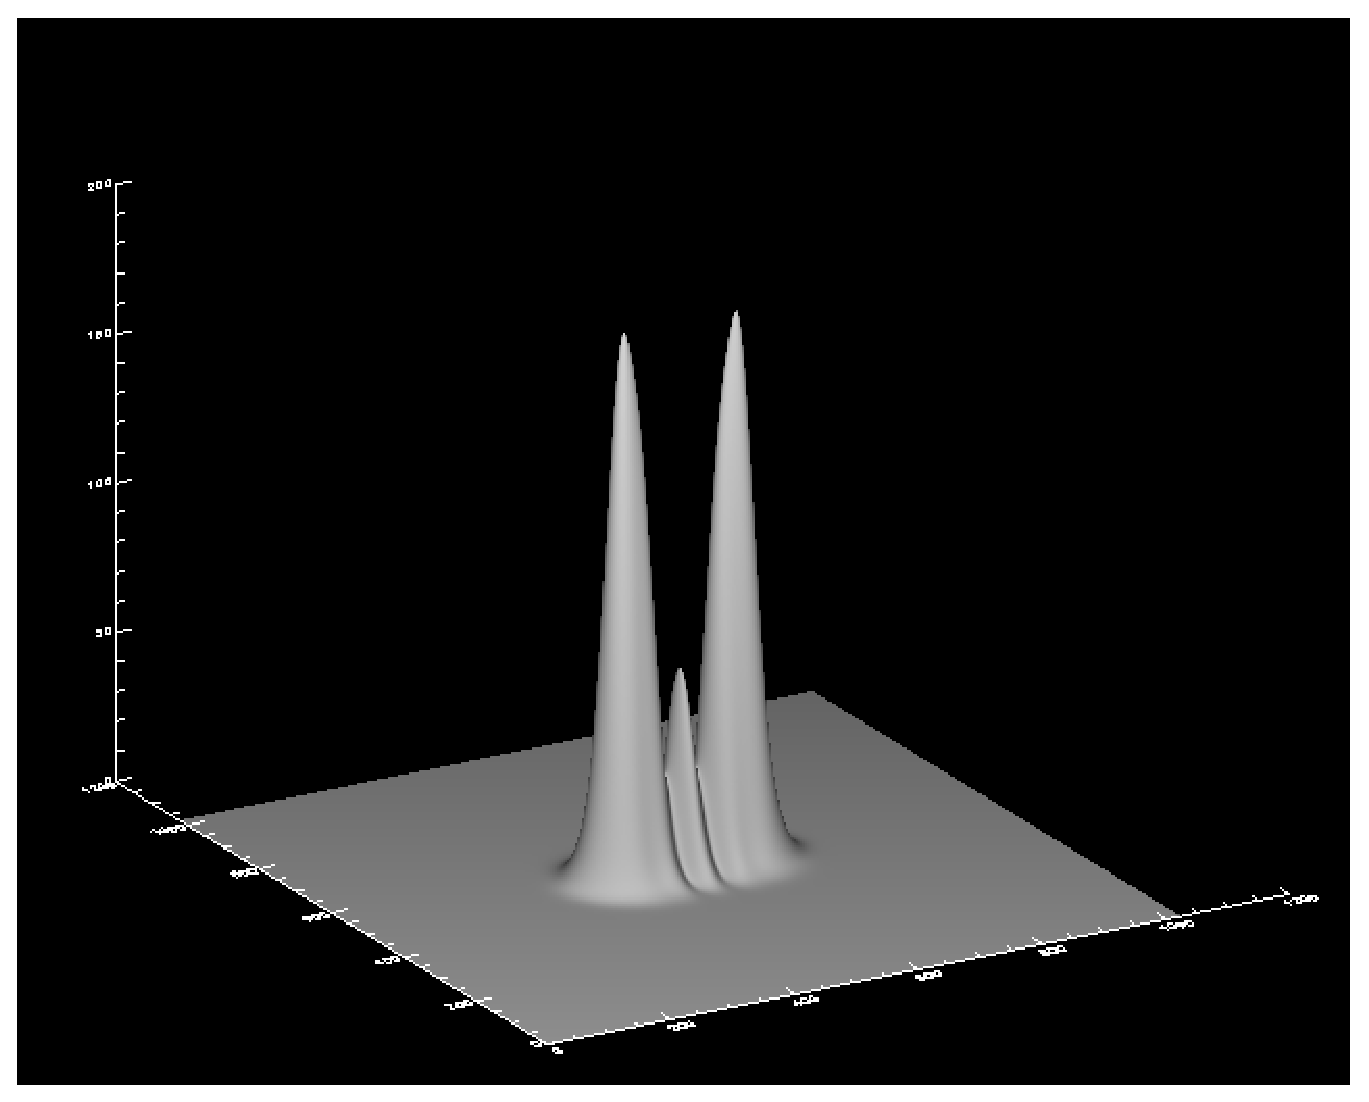
\includegraphics[width=0.49\columnwidth]{./full/twobody/deltas_035}

   \end{center}
\caption{The plots here show two gaussian wave-packets ($\psi^* \psi$, which is density) interacting under gravity. The output times are $0, 10, 15, 25, 30, 35$, they show the start of the simulation where the two peaks are attracted towards each other.}
\label{fig.twobody}
\end{figure}

\begin{figure}[htb]
   \begin{center}
     %\leavevmode
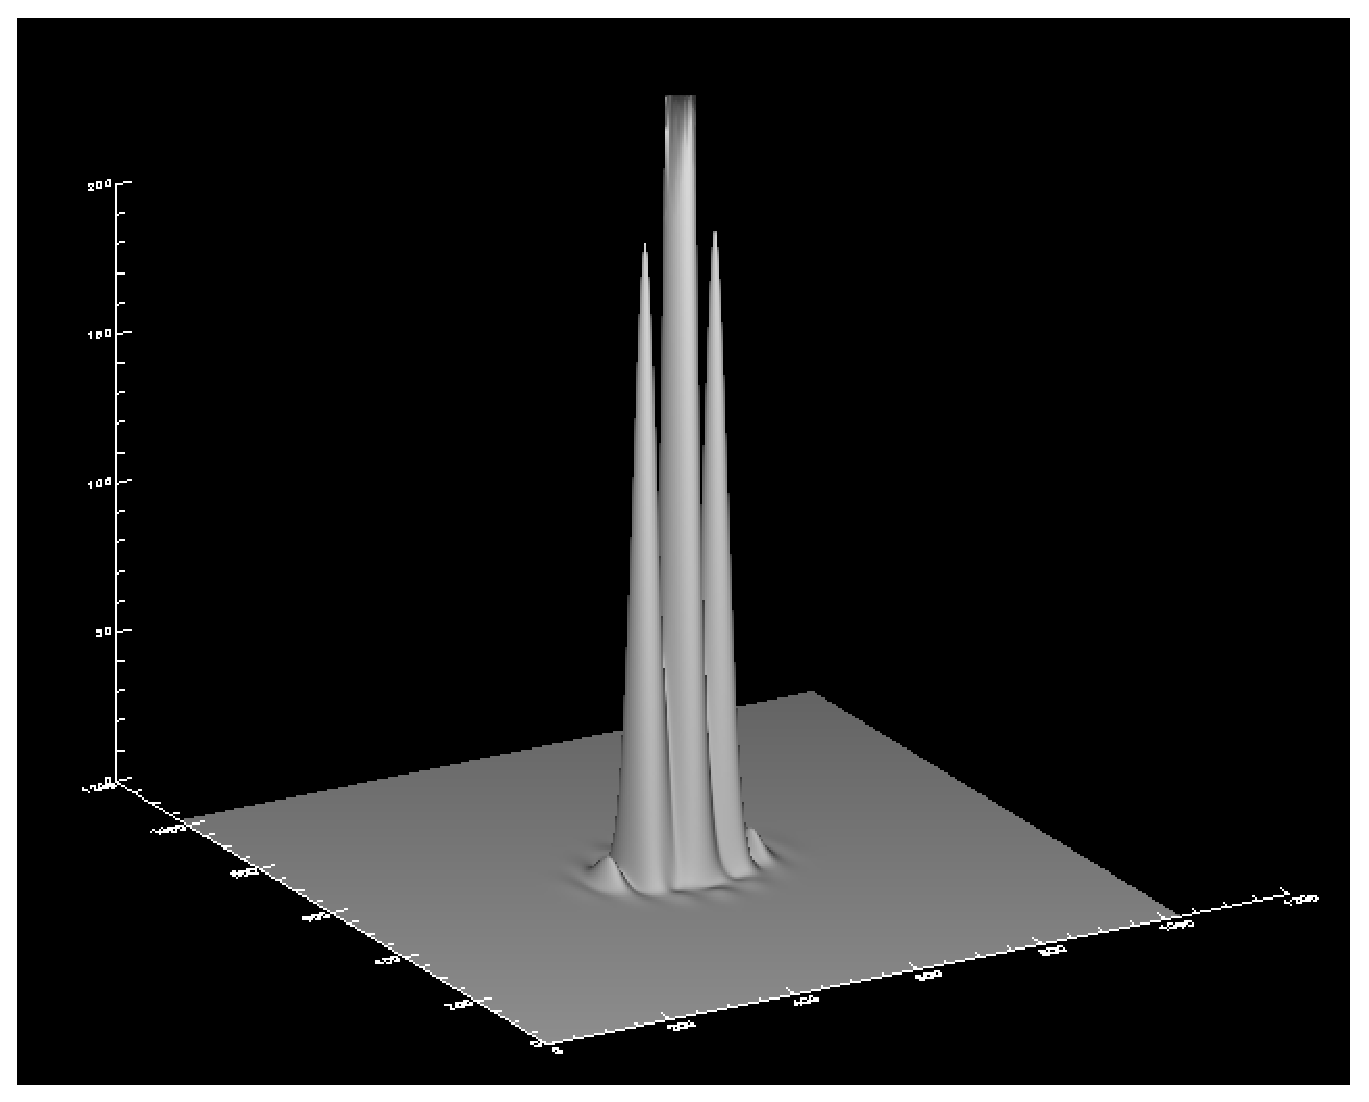
\includegraphics[width=0.49\columnwidth]{./full/twobody/deltas_040}
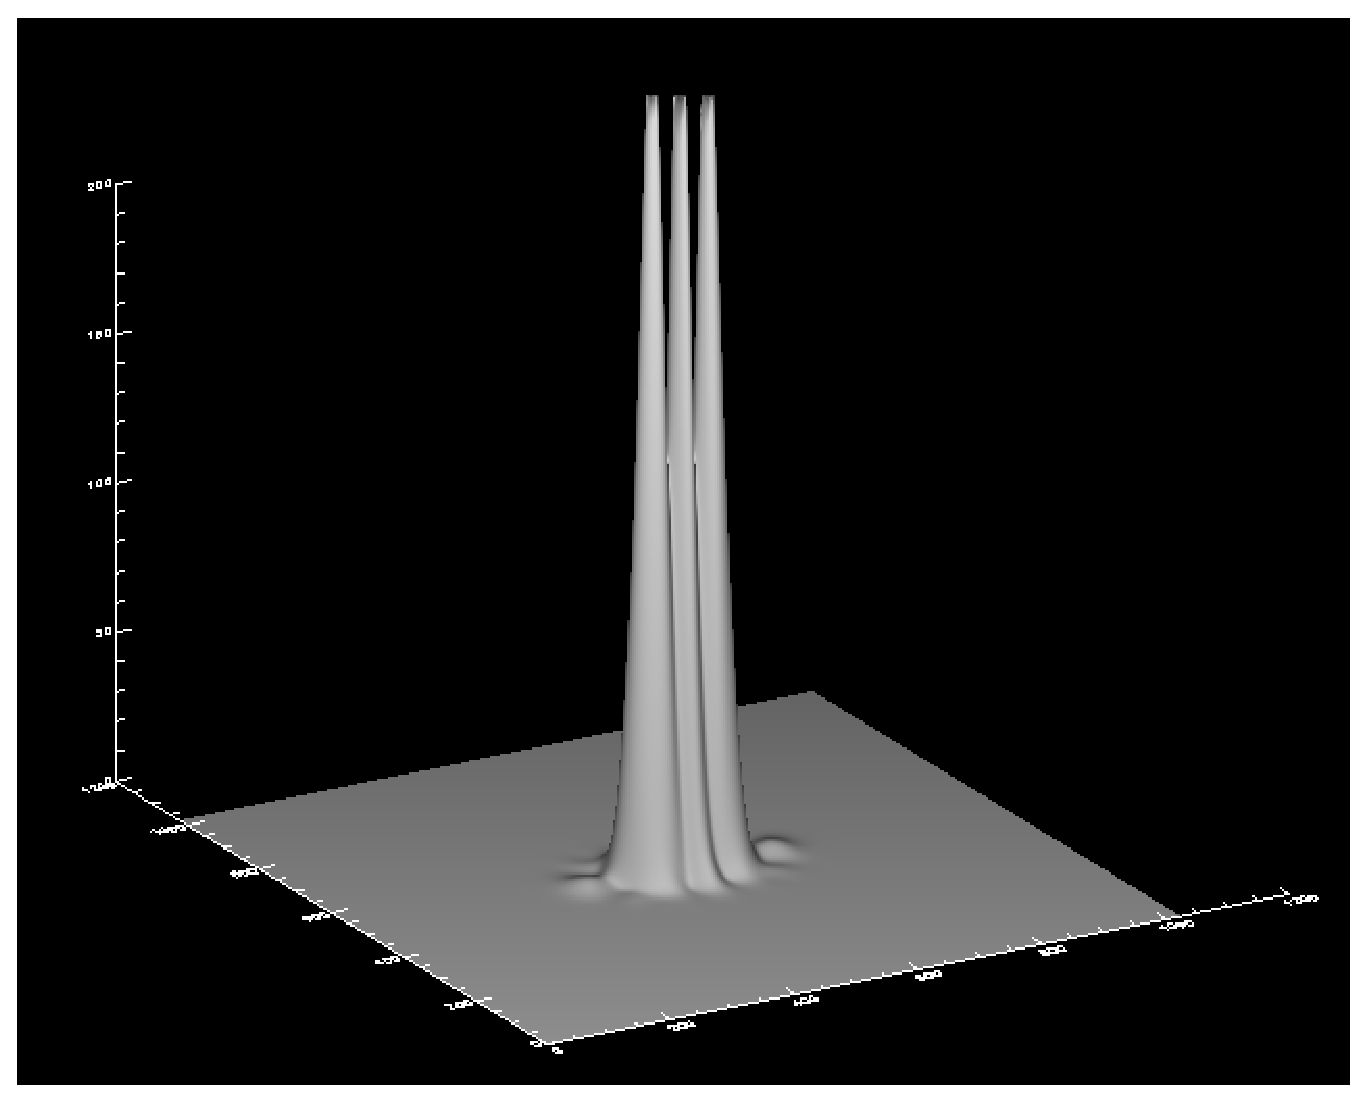
\includegraphics[width=0.49\columnwidth]{./full/twobody/deltas_045}
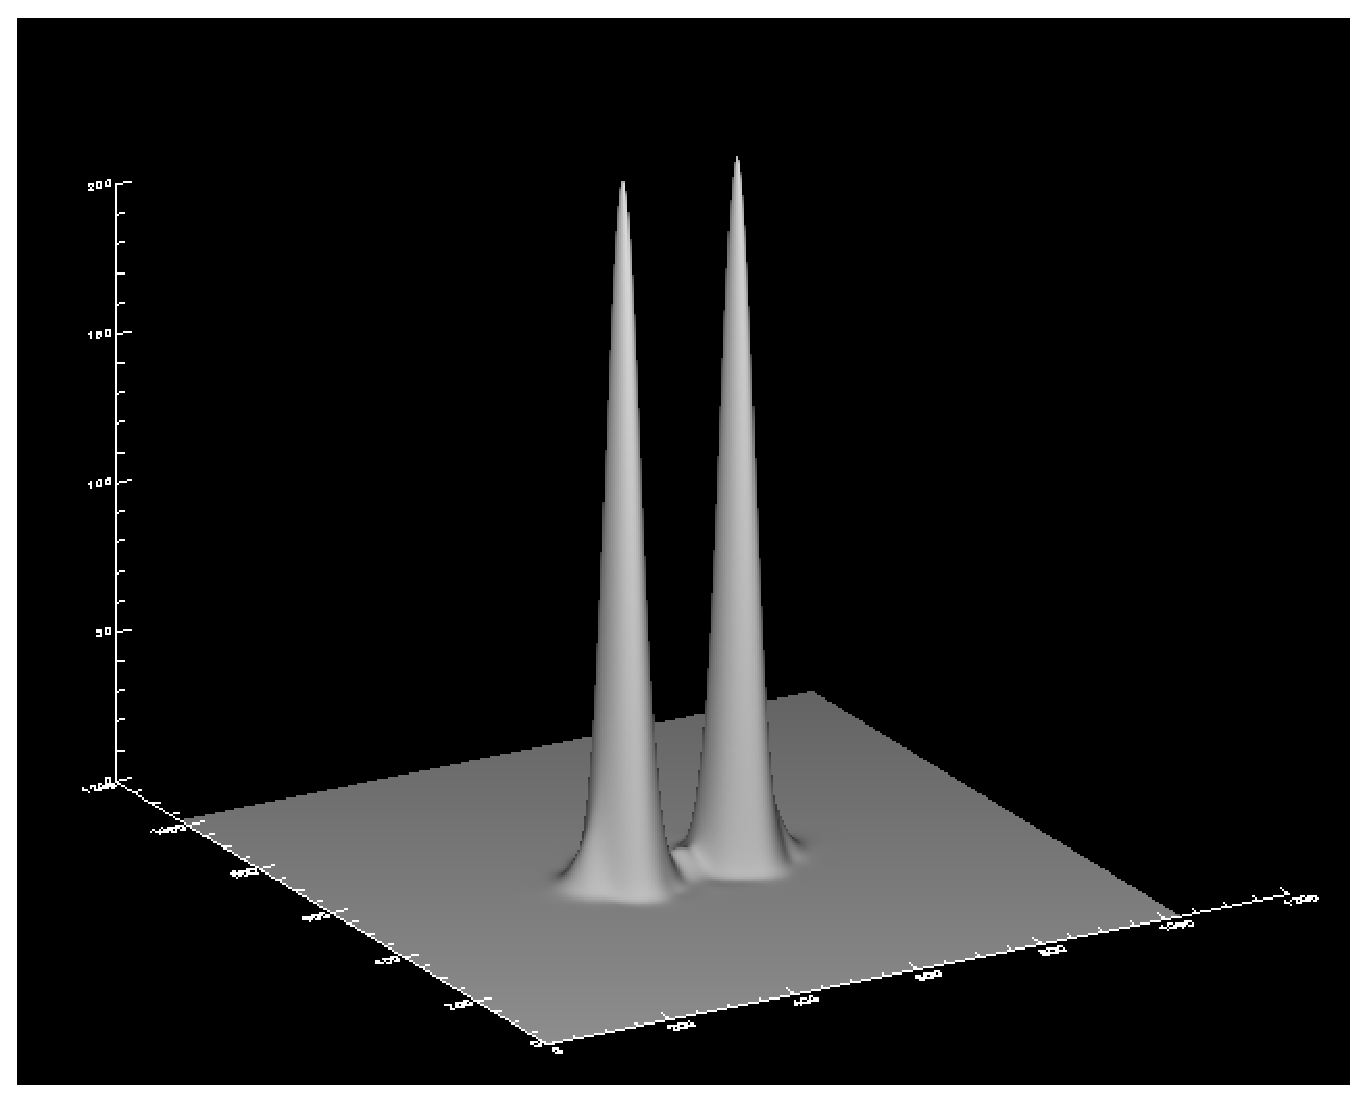
\includegraphics[width=0.49\columnwidth]{./full/twobody/deltas_050}
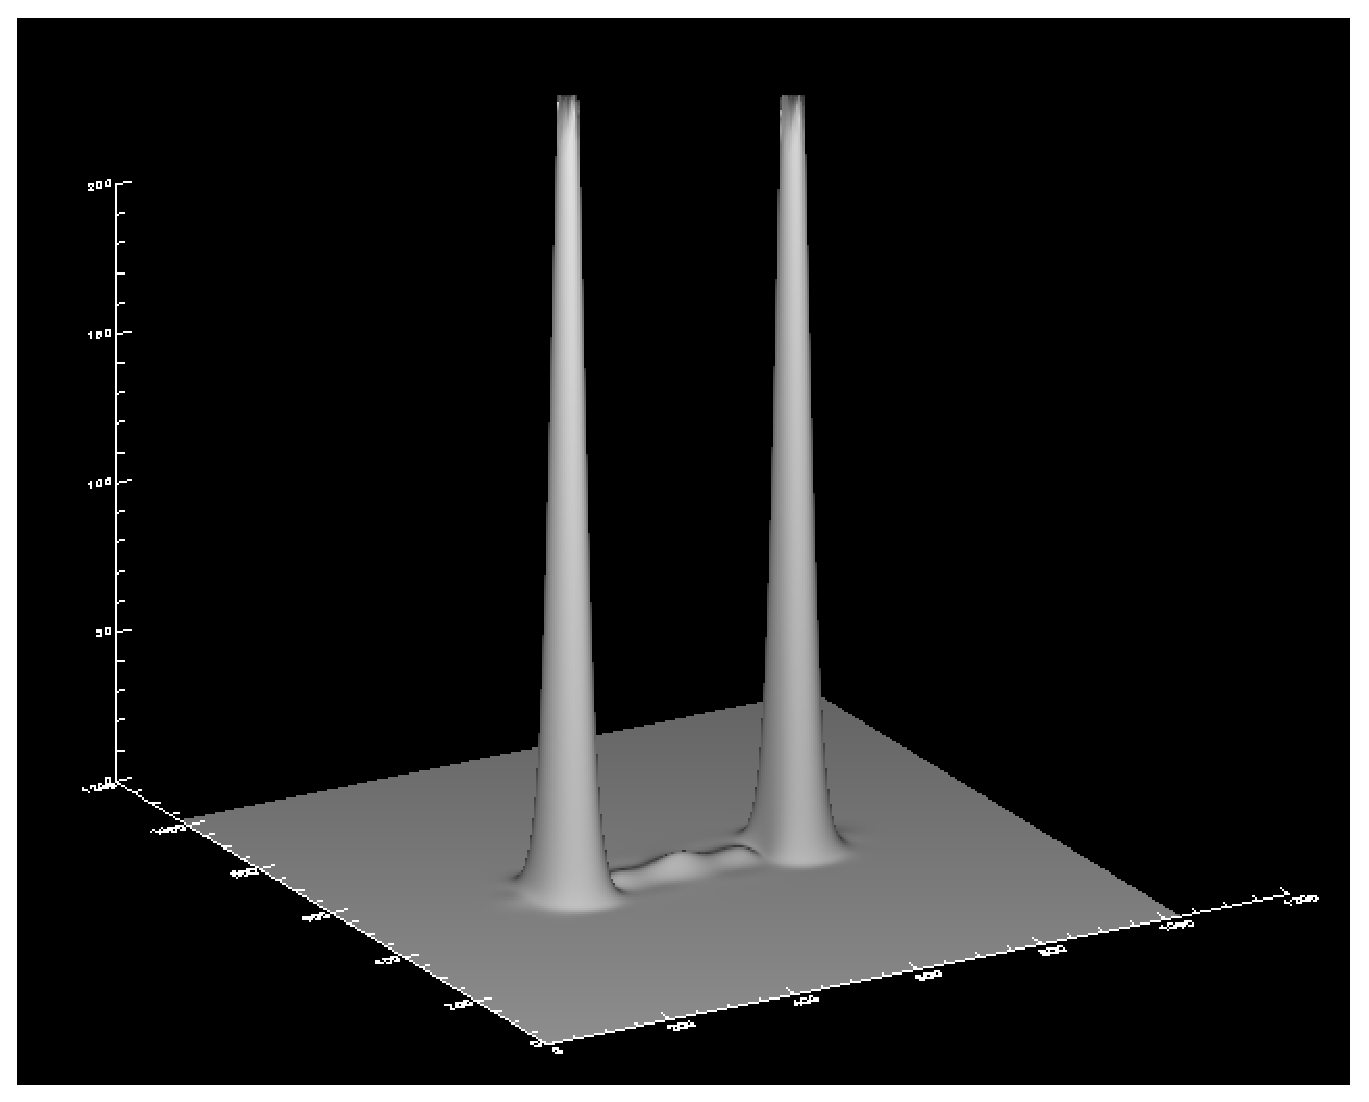
\includegraphics[width=0.49\columnwidth]{./full/twobody/deltas_065}
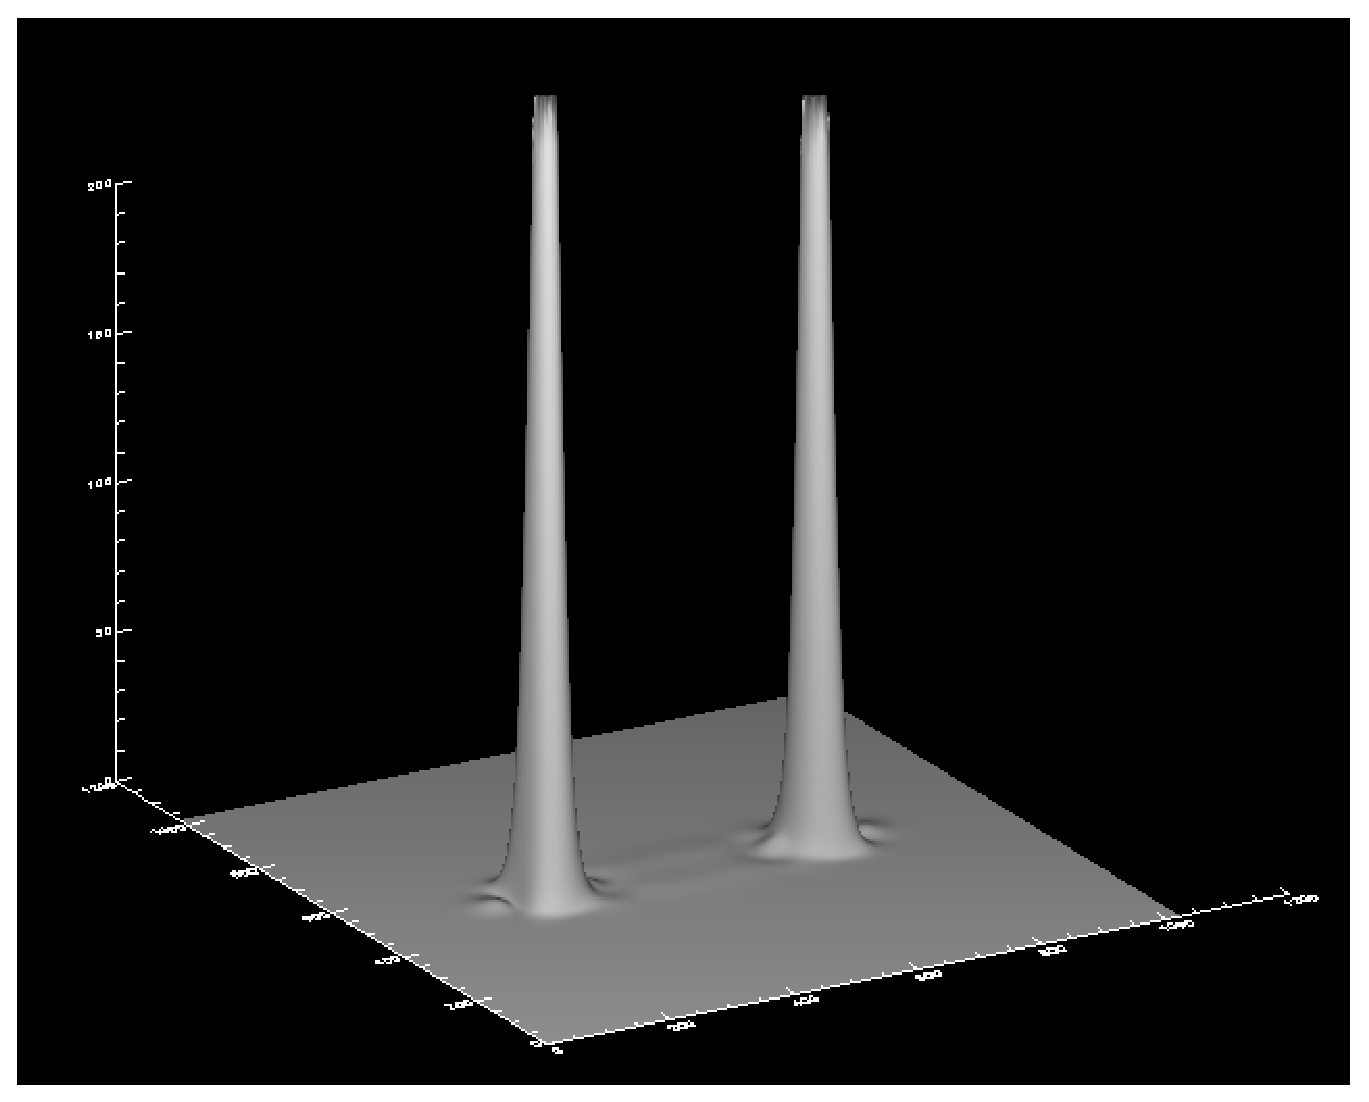
\includegraphics[width=0.49\columnwidth]{./full/twobody/deltas_080}
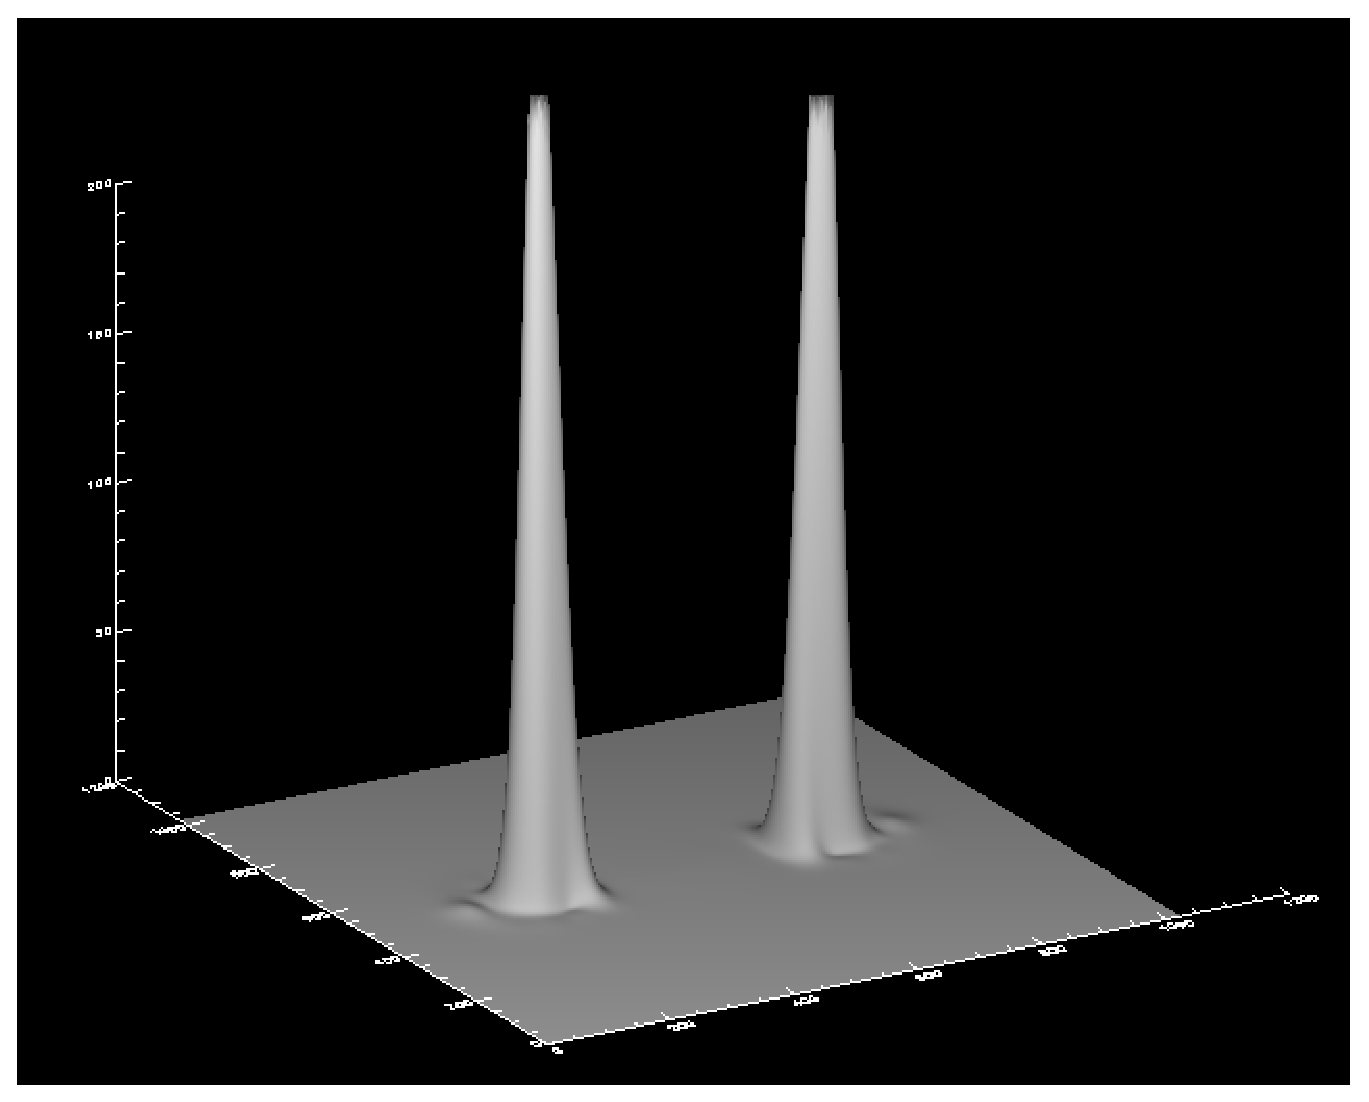
\includegraphics[width=0.49\columnwidth]{./full/twobody/deltas_100}

   \end{center}
\caption{In these plots we can see the two waves pass through each other. The waves collide in the first plot and are then shown to have fully passed through each other in the last plot. The output times are at timesteps of $40, 45, 50, 65, 80, 100$.}
\label{fig.twobody2}
\end{figure}

\begin{figure}[htb]
   \begin{center}
     %\leavevmode
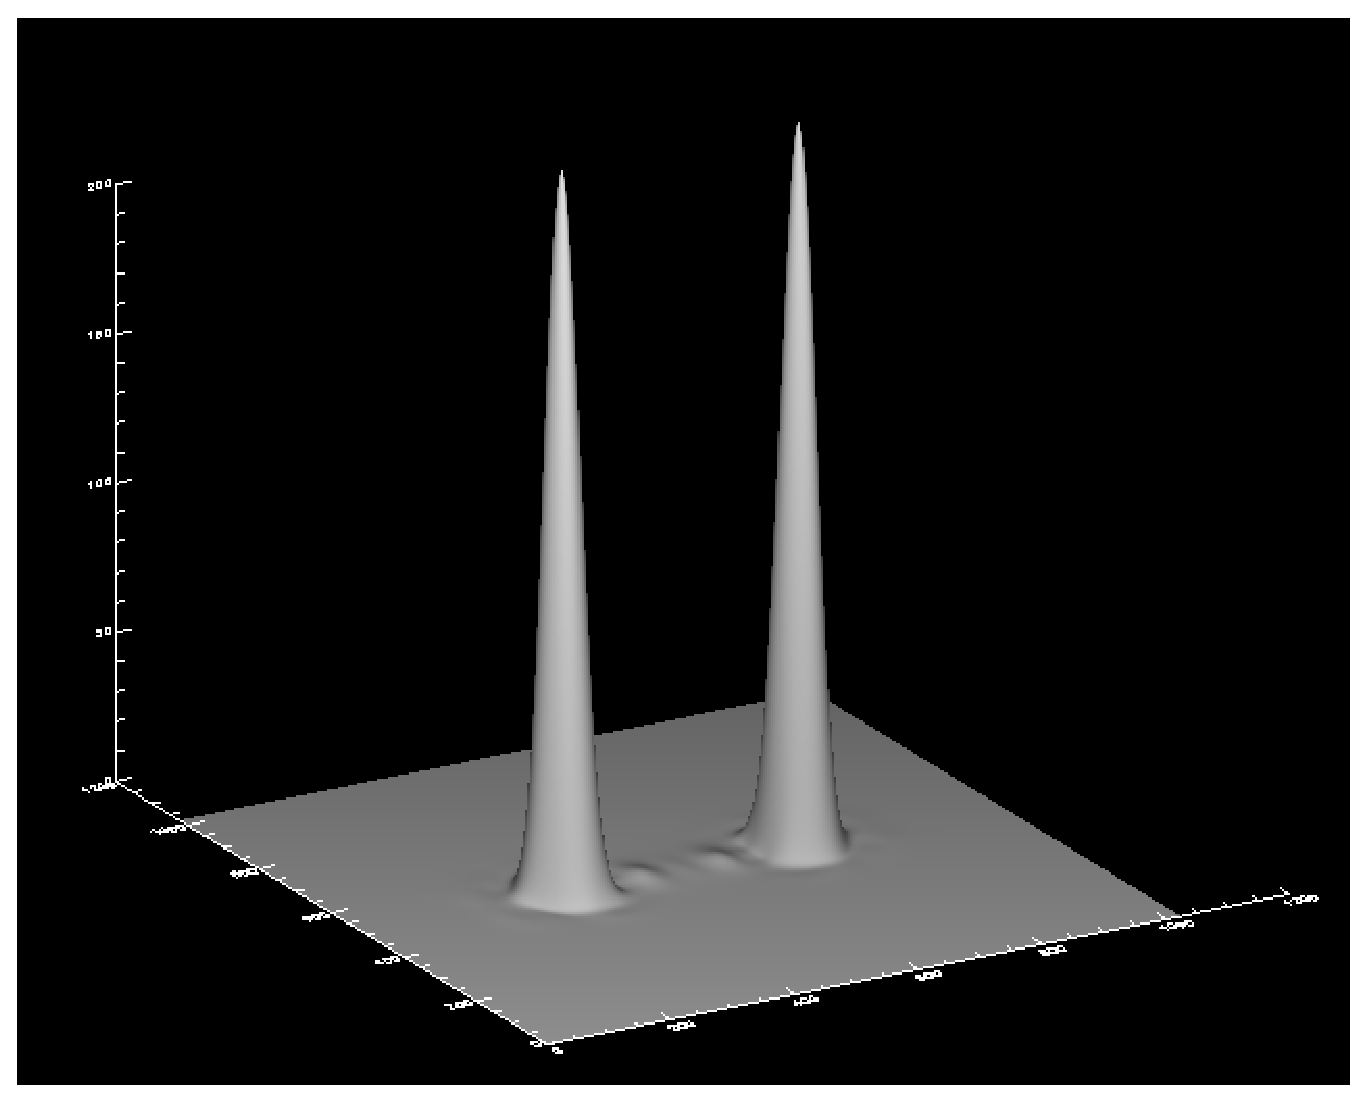
\includegraphics[width=0.45\columnwidth]{./full/twobody/deltas_120}
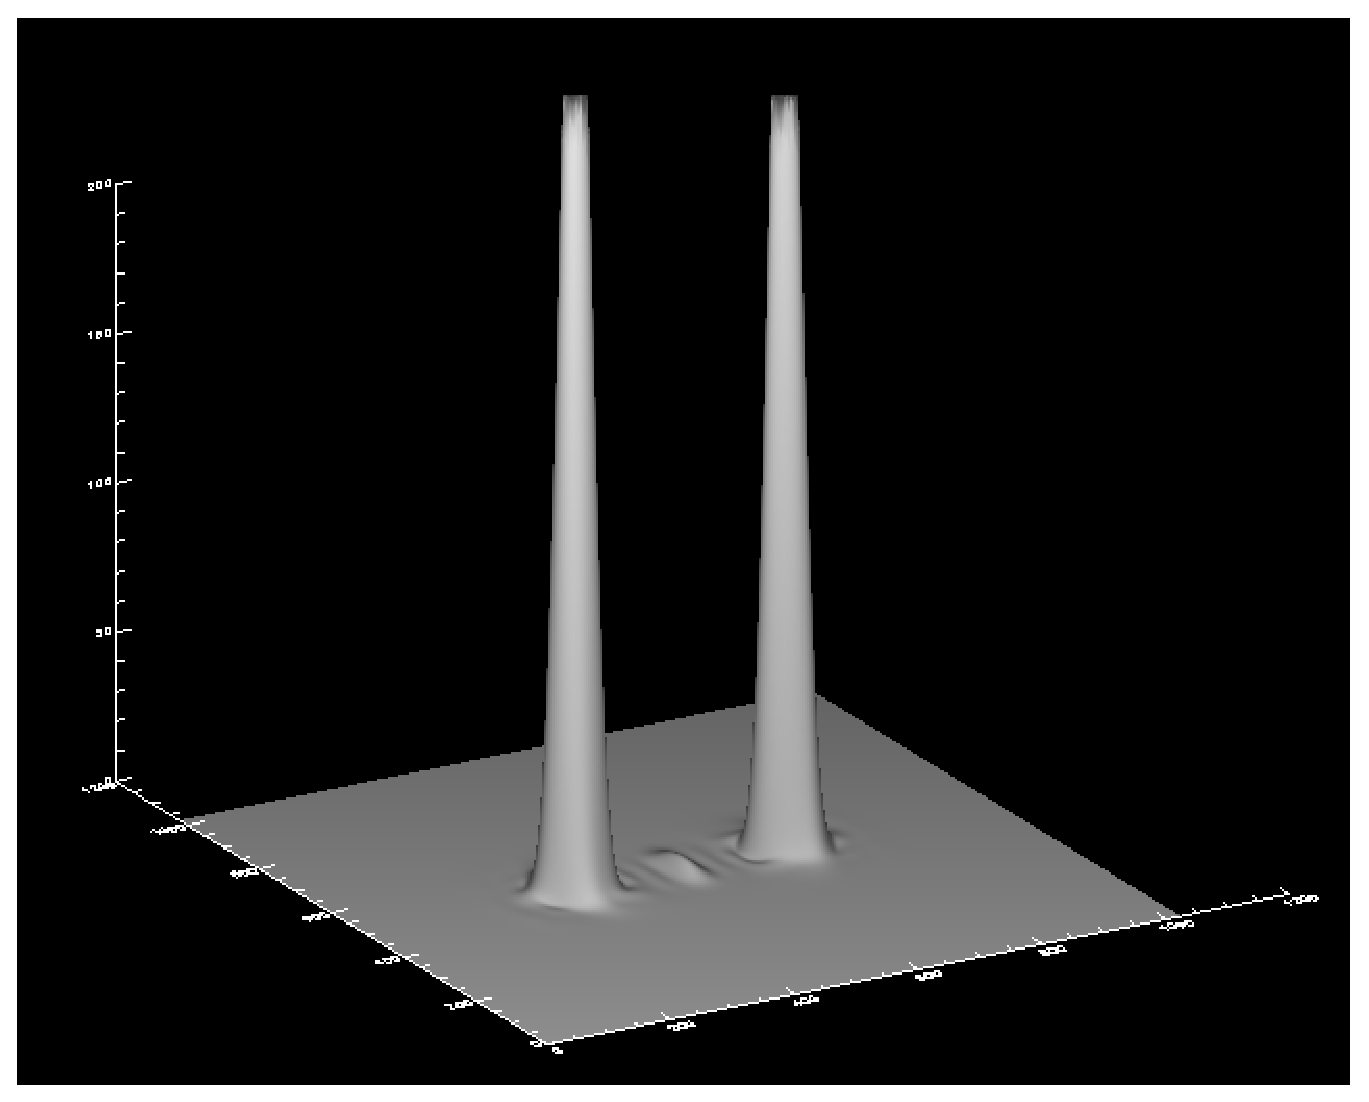
\includegraphics[width=0.45\columnwidth]{./full/twobody/deltas_125}
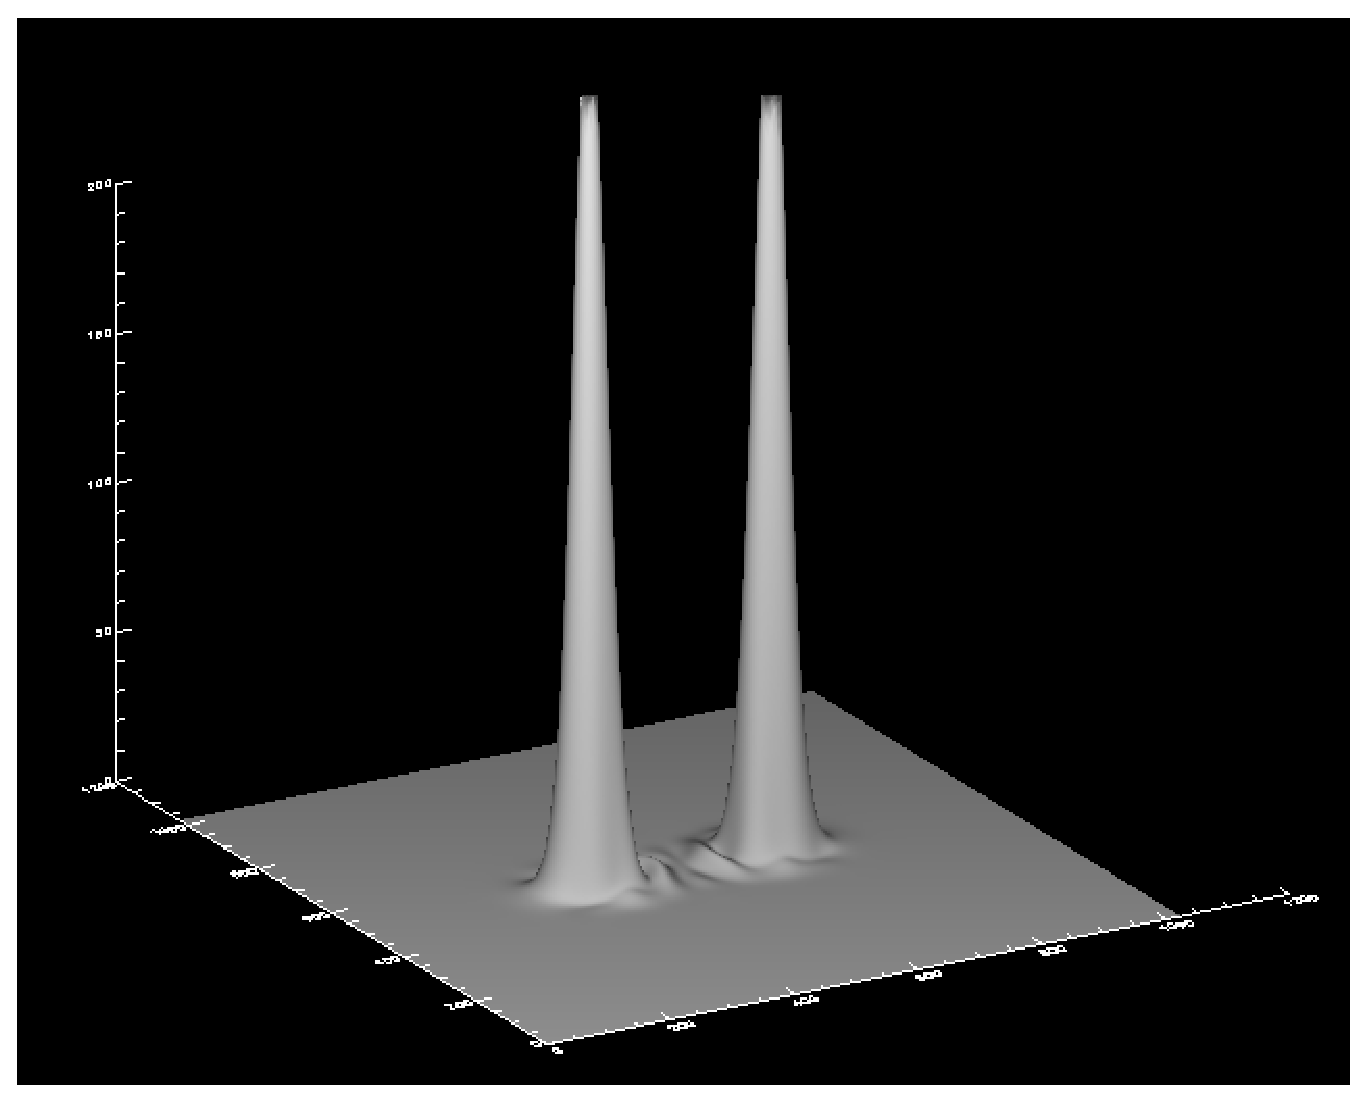
\includegraphics[width=0.45\columnwidth]{./full/twobody/deltas_130}
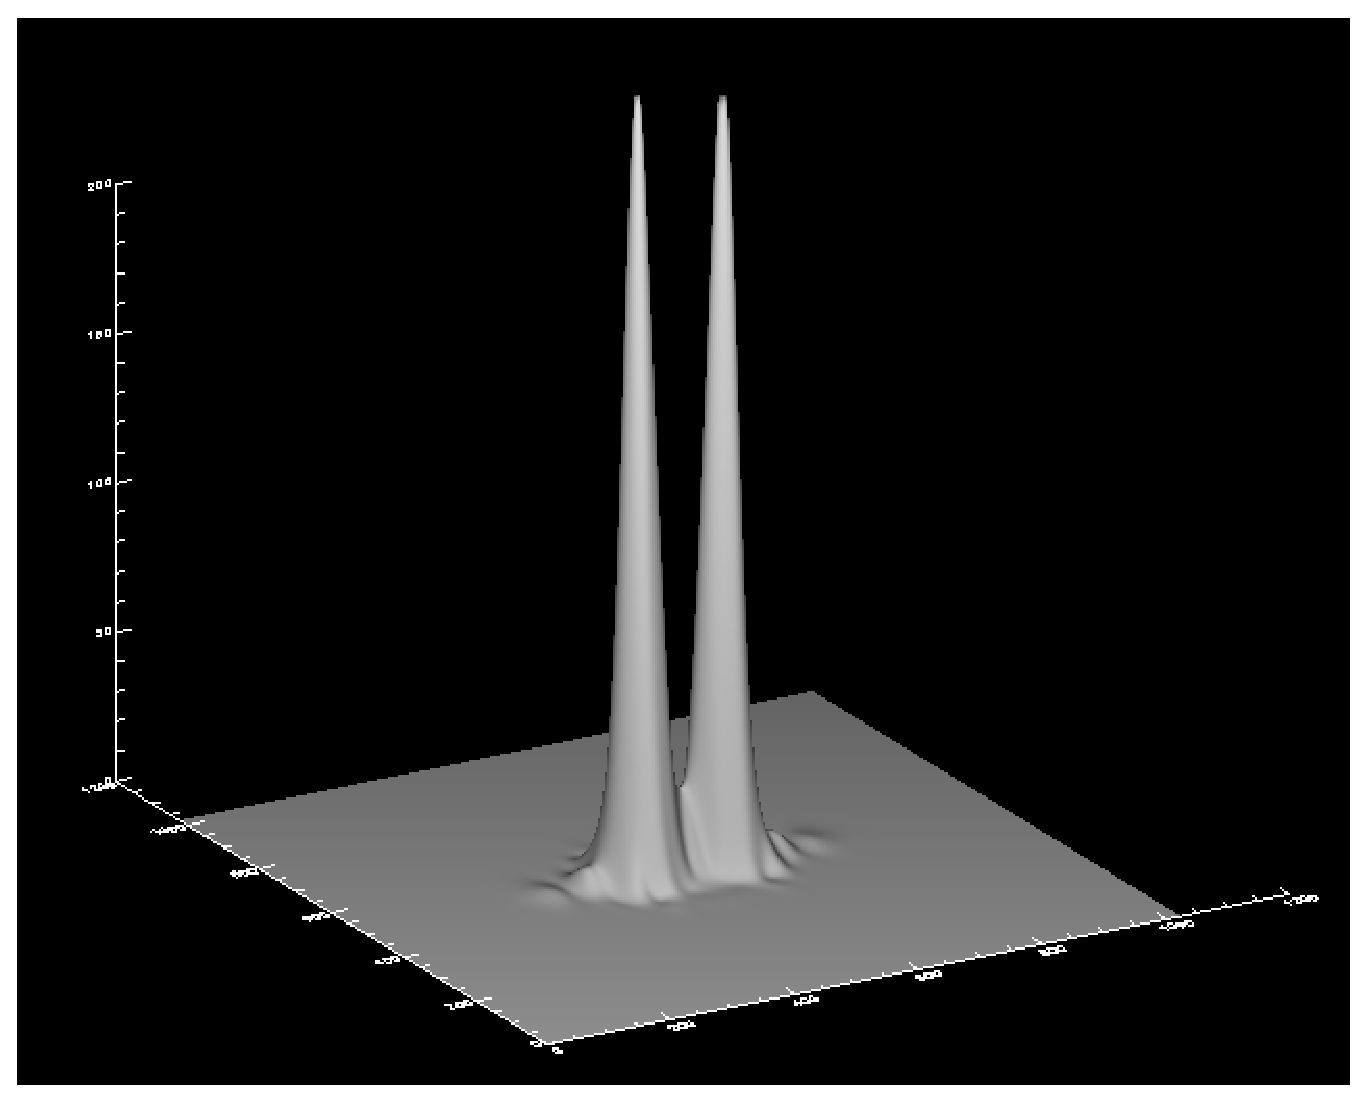
\includegraphics[width=0.45\columnwidth]{./full/twobody/deltas_140}
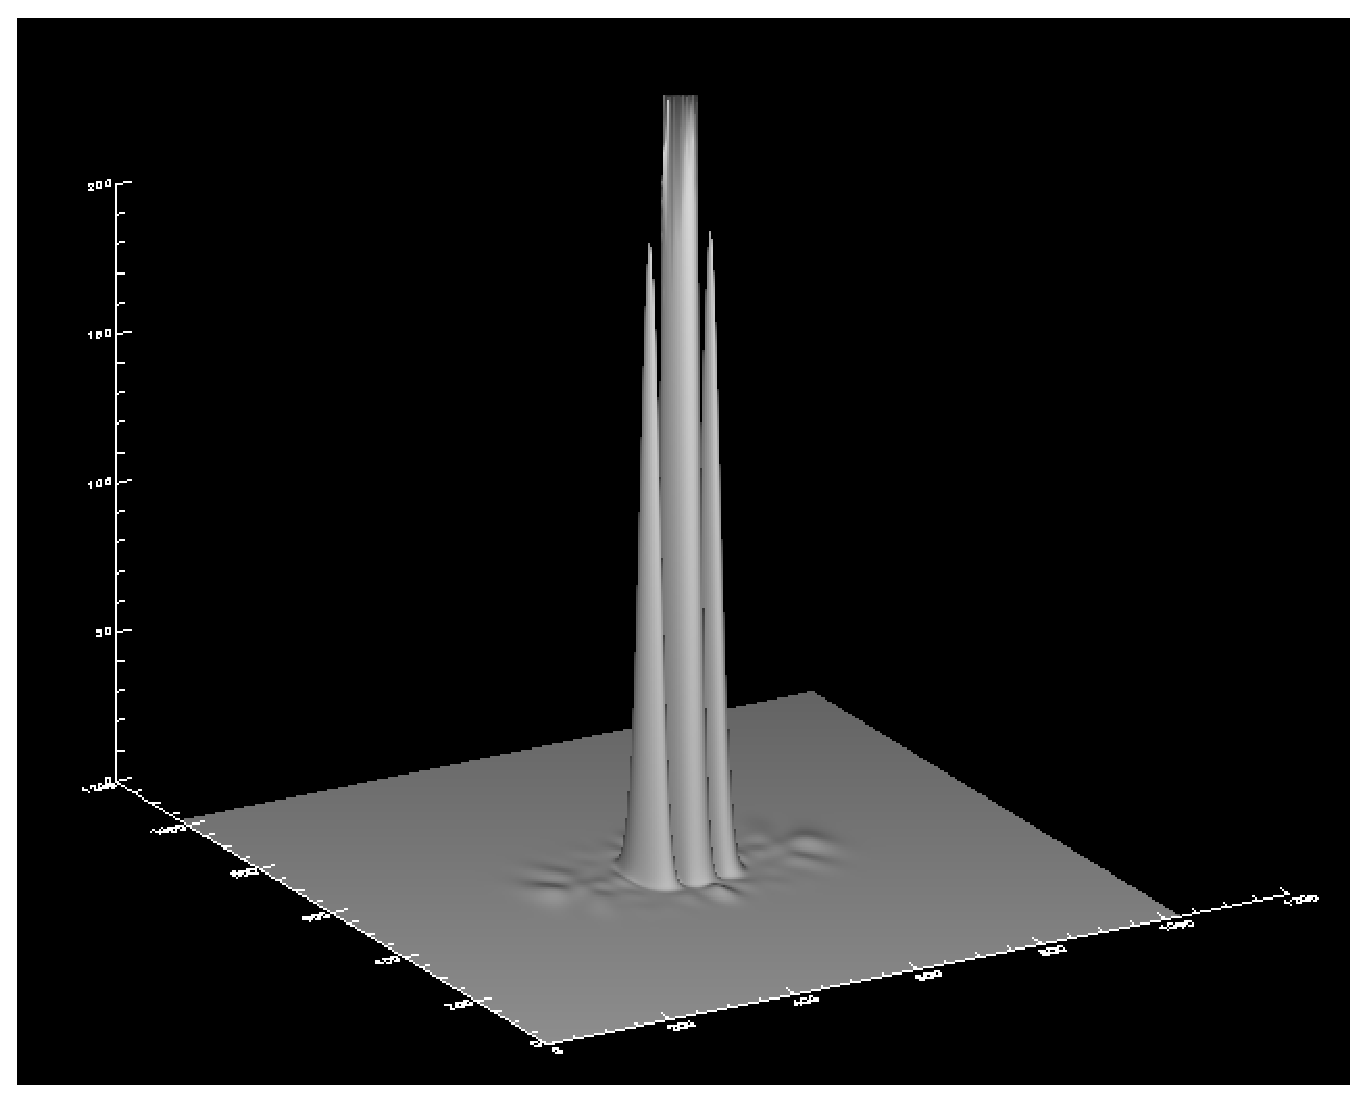
\includegraphics[width=0.45\columnwidth]{./full/twobody/deltas_145}
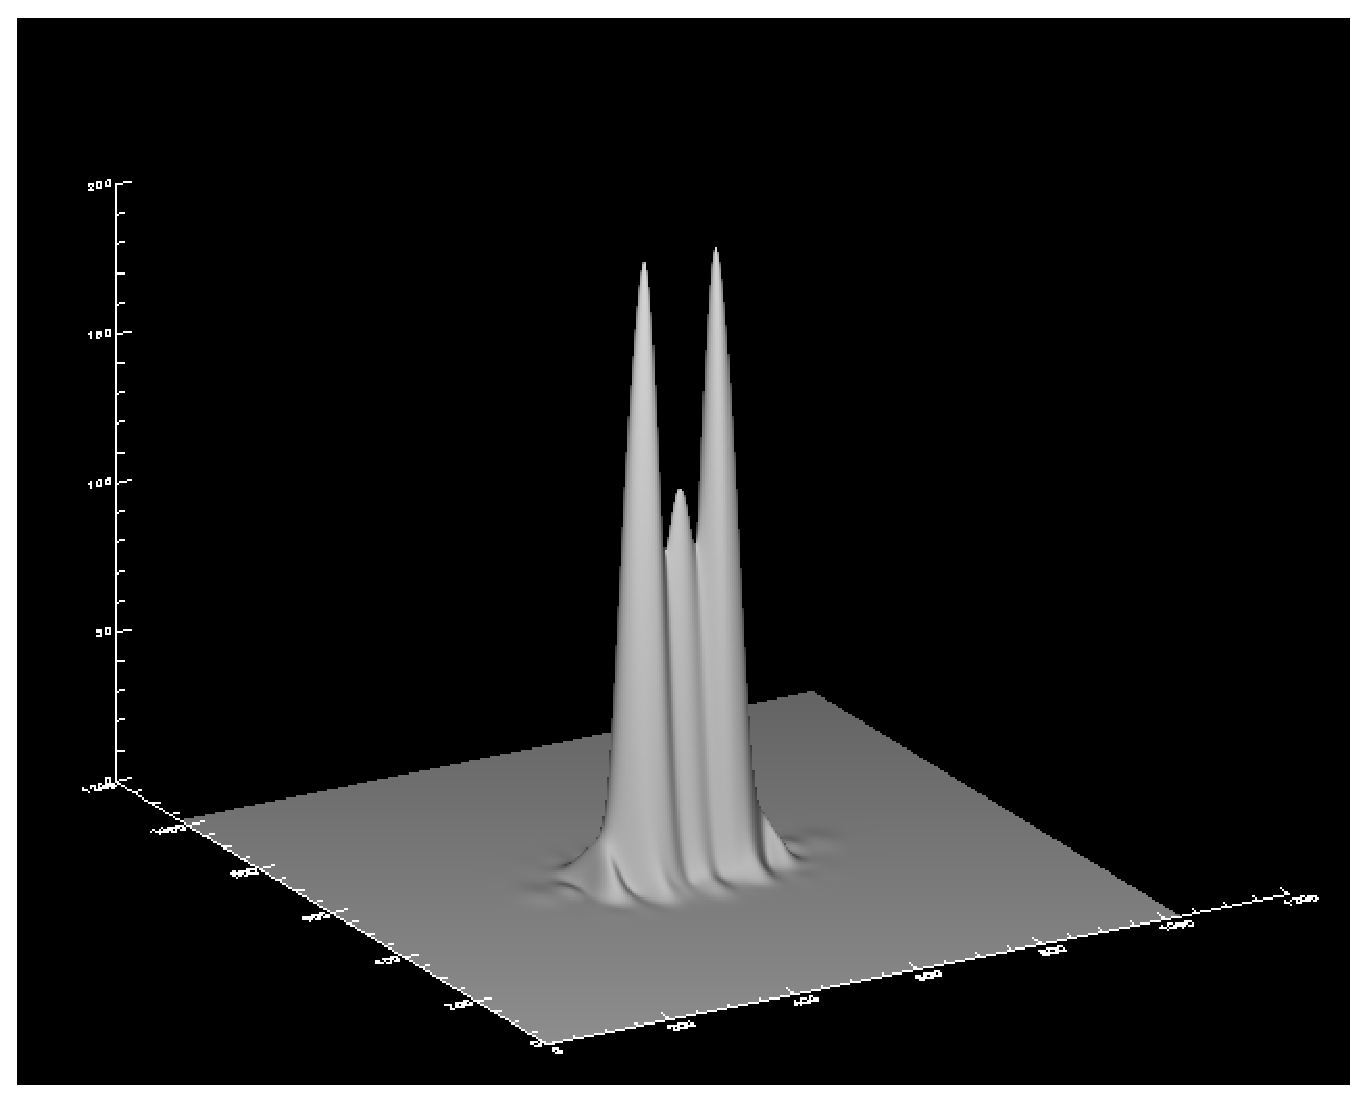
\includegraphics[width=0.45\columnwidth]{./full/twobody/deltas_150}

   \end{center}
\caption{These plots show that after the peaks have passed through each other they will turn around and collapse again. The pattern is similar to before but with some slight differences as noted in results section. The output times are $120, 125, 130, 140, 145, 150$.}
\label{fig.twobody3}
\end{figure}



\subsection{Tophat collapse}
\label{tophat}
The two-body interaction was a test of the gravitational routine, while the test of the tophat collapse will test gravity as well as expansion. Implicitly assumed so far, as in all 3D tests, is the use of splitting operators for implementing wave-mechanics in more than one spatial dimension. The code used here is one that will be used to conduct the full cosmological simulations; hence it is 3D, has periodic boundary conditions, includes self-consistent gravity and cosmological expansion.

The tophat collapse is a classic test of $N$-body codes. Due to the high symmetry of the problem then it is one of the simplest models for analysing non-linear evolution (Coles, \citep{bib_pcoles}). As Coles notes, the tophat is ``not directly relevant to interesting cosmological models because the real fluctuations are expected to be highly irregular and random."

In an $N$-body code then the dynamics will be determined by the cosmological parameters chosen as well as the distribution of the mass. In wave-mechanics there is, as always, one more parameter to consider: the $\nu$ parameter that determines the speed of dispersion as outlined before (section \ref{hydro}). When the mass distribution of the tophat is tall (relative to background density) and thin then collapse will happen more quickly. For a distribution that is short and flat then collapse is suppressed.

The parameters used in this test were: $H_0 = 72, a_i = 0.04, \Omega = 1, \Omega_{m,0} = 0.3, L = 100 {\rm Mpc/h}, \nu = 10^{-8}$. The resolution used is $64^3$ gridpoints where a central over-density that is 8 pixels in diameter and is at a level of $\delta = 2$. See figure \ref{fig.tophat} for the resultant plots.

The results show that the over-density collapses to a nearly singular point by timestep 1800 ($\delta = 6.67$) , the over-density grows until a maximum peak of $\delta = 8.33 $ at timestep 2200. From there it stays at that peak until the end of the simulation (timestep 3200) in an apparently static state.

As point of comparison, we will provide an alternative set of plots (figure \ref{fig.tophat2}) that use a larger value of $\nu$ ($10^{-7}$). This alternative set of plots shows that collapse happens faster, as is expected from using a higher value of $\nu$. The parameters were otherwise held constant, that is to say that we used the same initial conditions. Collapse to the same peak ($\delta = 8.33 $) has now occurred by timestep 800; however, the peak soon drops in height and fattens until the end of the simulation. The over-density is still centralized but it appears that gravity is not strong enough to hold the region as a quasi-singular point of density. In tests where $\nu$ is much larger the over-density expands so fast that the wavefunction crosses over the boundaries. This provides feedback into the system where different frequencies within the wavefunction can cause an interference pattern. The result is an unsmooth wavefunction with rapid variability.


\begin{figure}[htb]
   \begin{center}
     %\leavevmode

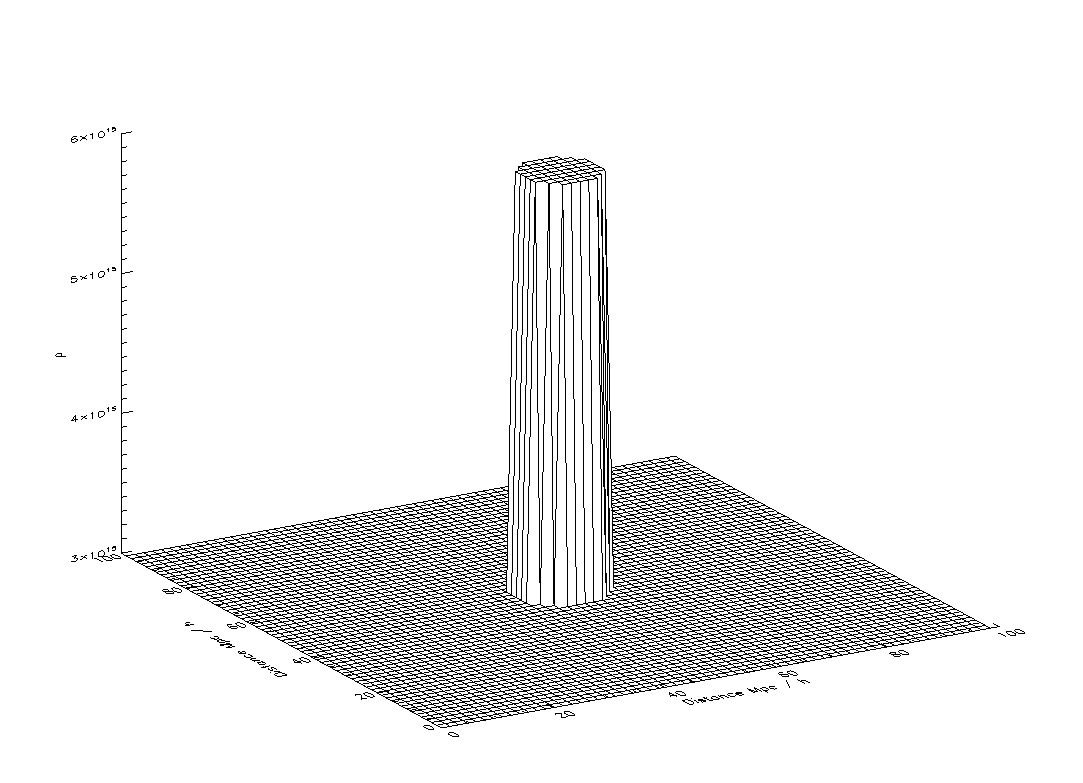
\includegraphics[width=0.49\columnwidth]{./full/tophat/nu_-8--5/tophat.eps}
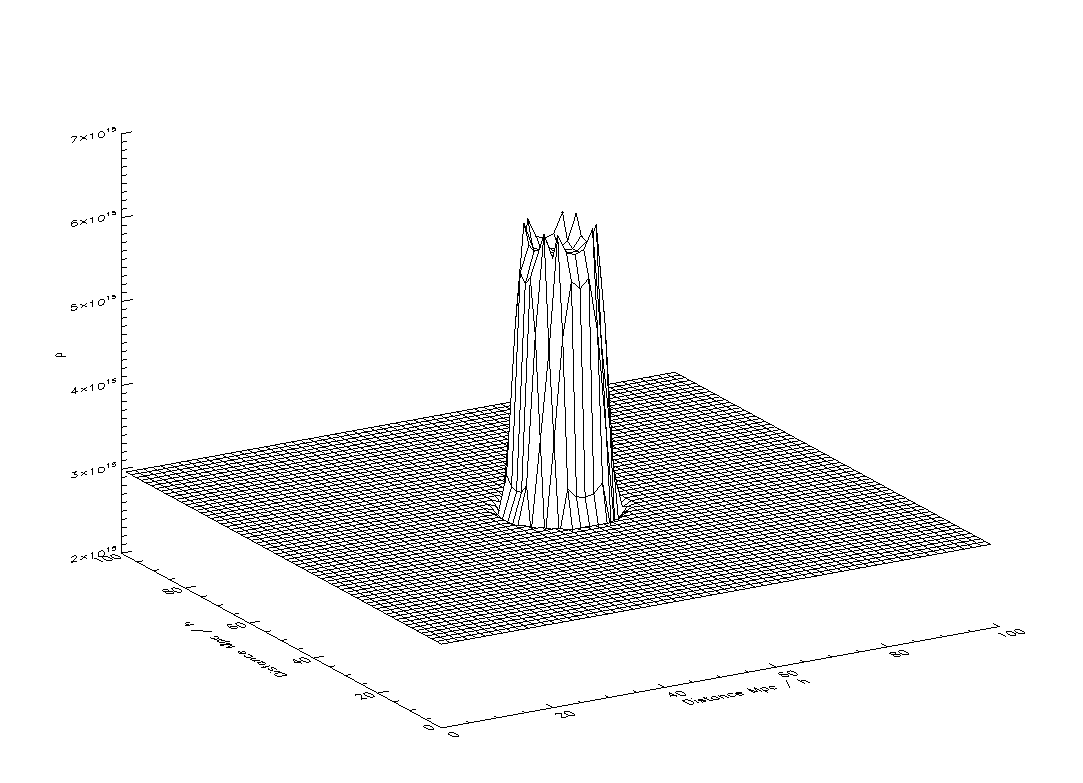
\includegraphics[width=0.49\columnwidth]{./full/tophat/nu_-8--5/rho_evs_00200.eps}

\includegraphics[width=0.49\columnwidth]{./full/tophat/nu_-8--5/rho_evs_00600.eps}

\includegraphics[width=0.49\columnwidth]{./full/tophat/nu_-8--5/rho_evs_1000.eps}

\includegraphics[width=0.49\columnwidth]{./full/tophat/nu_-8--5/rho_evs_2000.eps}

\includegraphics[width=0.49\columnwidth]{./full/tophat/nu_-8--5/rho_evs_3000.eps}
   \end{center}
\caption{The (comoving) plots here show a $2D$ slice of a $3D$ tophat collapse. The top left plot shows the initial condition ($a = 0.04, \delta = 0.1, \nu = 10^{-8}$). The plots (left to right) are $t = 0, 200, 600,$ $1000, 2000, 3000$ ($a= 0.04, 0.05,$ $0.07, 0.1, 0.3, 0.8$).}
\label{fig.tophat}
\end{figure}

\begin{figure}[htb]
   \begin{center}
     %\leavevmode

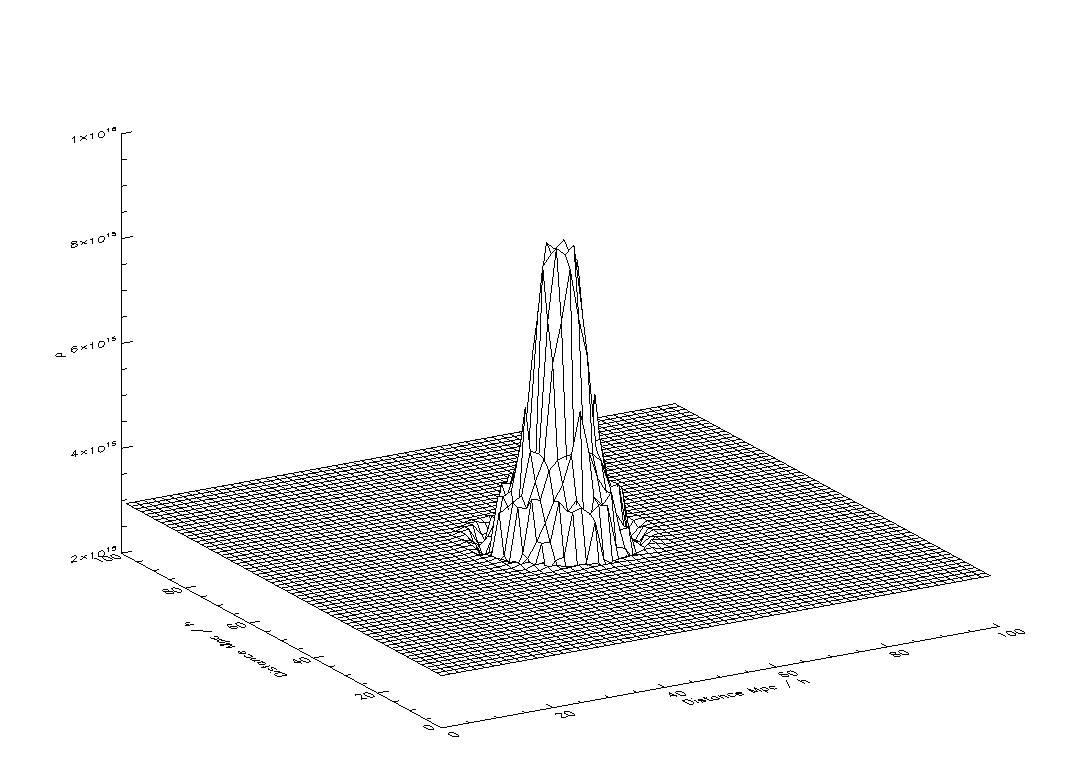
\includegraphics[width=0.49\columnwidth]{./full/tophat/nu_-7/rho_evs_00600.eps}
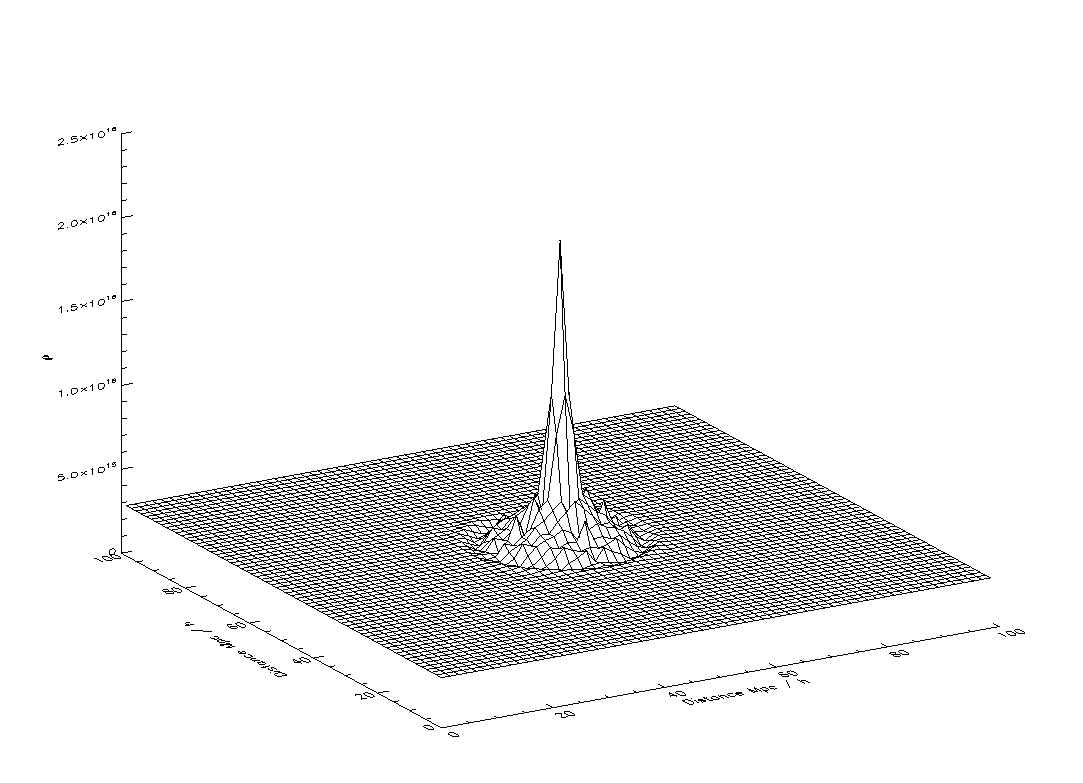
\includegraphics[width=0.49\columnwidth]{./full/tophat/nu_-7/rho_evs_00800.eps}
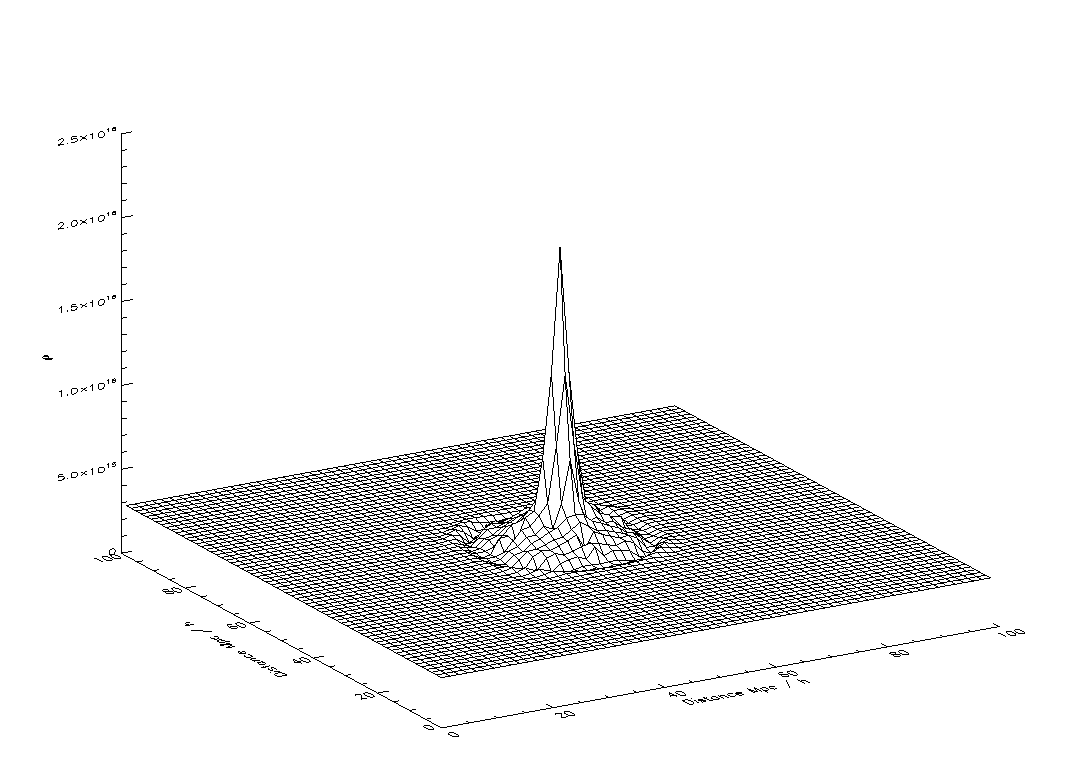
\includegraphics[width=0.49\columnwidth]{./full/tophat/nu_-7/rho_evs_1000.eps}
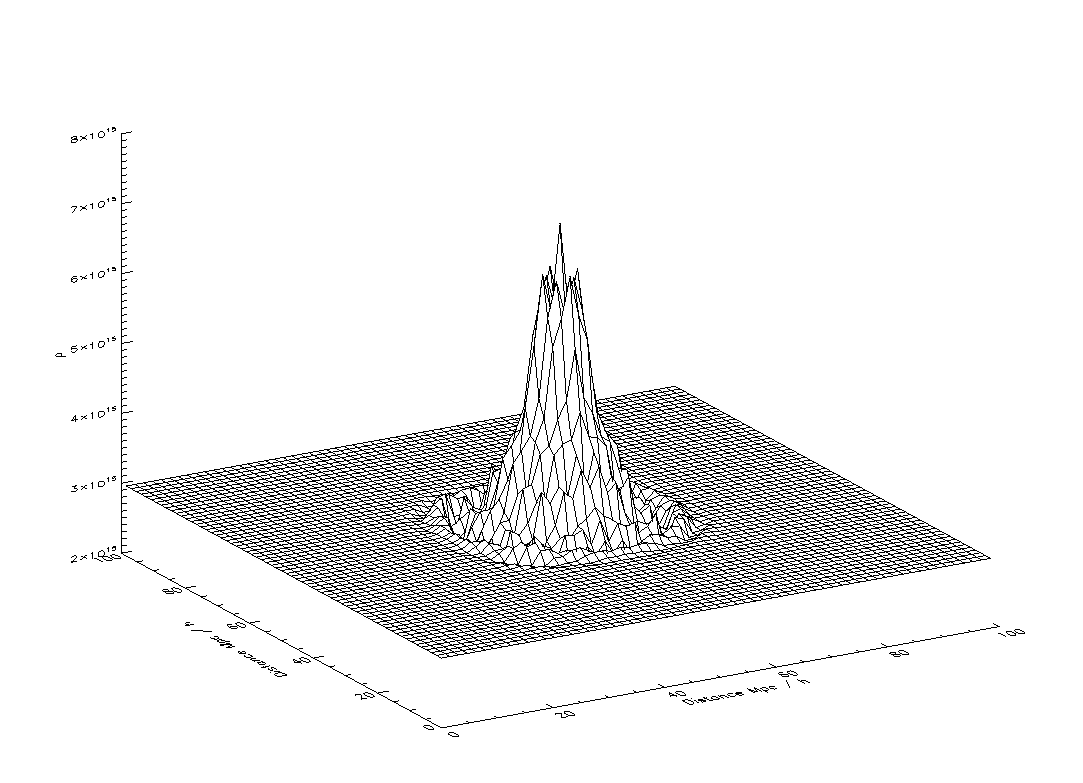
\includegraphics[width=0.49\columnwidth]{./full/tophat/nu_-7/rho_evs_1600.eps}
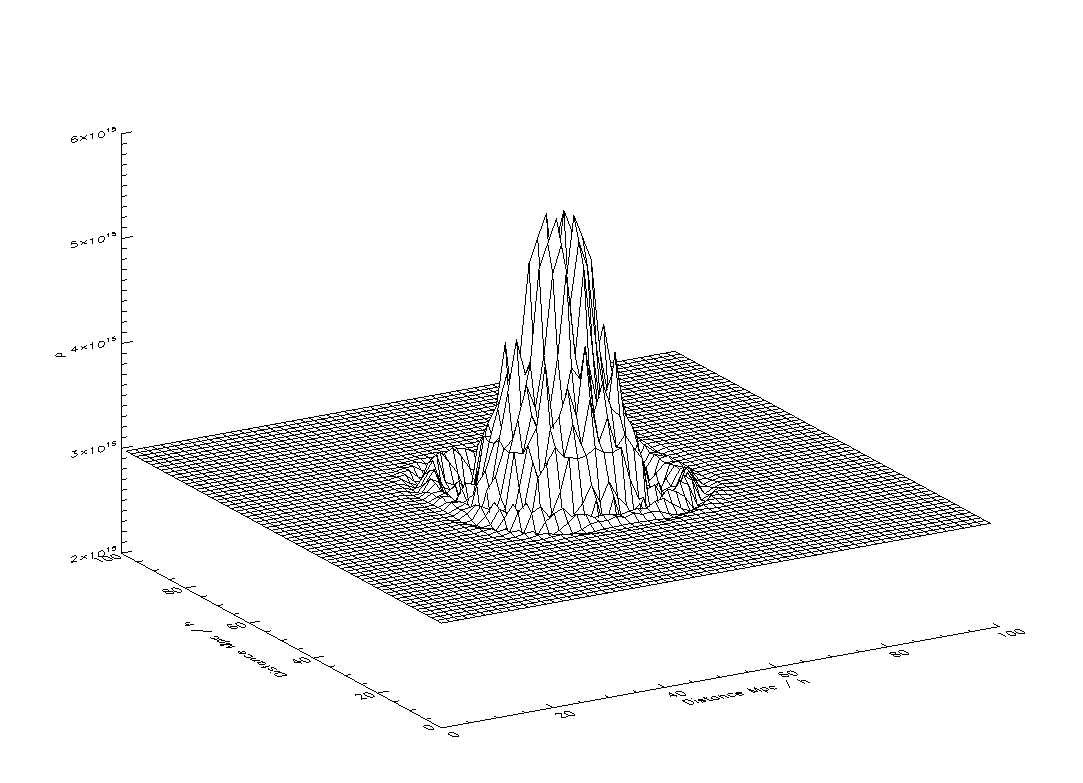
\includegraphics[width=0.49\columnwidth]{./full/tophat/nu_-7/rho_evs_2000.eps}
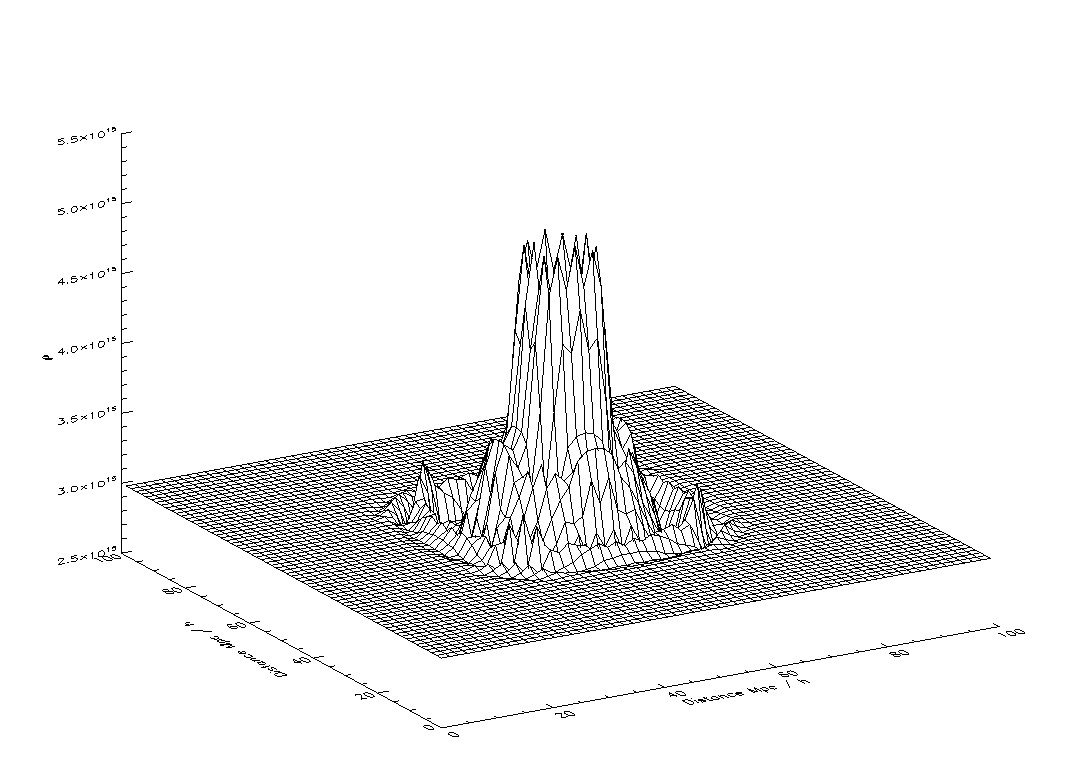
\includegraphics[width=0.49\columnwidth]{./full/tophat/nu_-7/rho_evs_3000.eps}
   \end{center}
\caption{Here is an alternative set of plots of a $3D$ tophat collapse. The top two plots show the initial condition ($a = 0.04, \delta = 0.1, \nu = 10^{-7}$) and the associated gravitational potential. The outputs are at times of $t = 600, 800, 1000, 1600, 2000, 3000$ ($a= 0.07, 0.09, 0.1, 0.19, 0.3, 0.8$).}
\label{fig.tophat2}
\end{figure}


\subsection{Cosmological simulation}
\label{cos_sim}
The key results of this thesis focus upon the application of the 3D code for one set of cosmological parameters, for various mass resolutions ($32^3 - 128^3$). The parameters are appropriate to a flat FLRW Universe and were chosen by Sabiu for his own purposes. Sabiu ran some $N$-body simulations and has donated his initial conditions files (at resolutions of $64^3$ and $128^3$ plus end time outputs for comparison with my wave-mechanics code. He generated initial conditions that were suitable for use with the code GADGET-2. These files include all the key cosmological parameters as well as the positions and velocities of all particles. The details of generating the initial conditions was presented in section \ref{cos_init}.

The process of generating initial conditions appropriate for a wave-mechanics code involves turning the particle positions into a continuous density field. To do this I used the Triangular Shaped Cloud (TSC) routine as provided by the Hydra $N$-body code, this code takes particle positions and outputs the number density. It constructs the density by performing a number count in each cell. This is then multiplied by the critical density of the Universe in order to construct a proper cosmological density field. From the density, a gravitational potential can be calculated using standard Fourier techniques (see \ref{sol_poi}) which is then used to create the initial wavefunction $\psi$. This seems like the fairest way to make a comparison with the industry standard, $N$-body, codes. It is not, however, the only way to create initial conditions.

Woo \& Chiueh \citep{bib_woo, bib_wooc} constructed their initial conditions by assuming the following form: $\psi = 1 + R + I$, where $R, I << 1$. The $R$ and $I$ are the real and imaginary perturbations about the mean value ($ = 1$) of the wavefunction. These perturbations are supposed to form a gaussian random field as required by cosmological structure theory. Such a method is attractive as if it can be done in a manner that faithfully represents a ``cosmological wavefunction" then it would avoid the necessity of smoothing particle positions. Performing this smoothing operation will inherently introduce error into the system as the particles positions were originally populated within an underlying smooth density field. Simply smoothing the positions will not give a completely faithful representation of the original field. An alternative possibility and perhaps the simplest approach would be to take the initially continuous density field from an initial condition generator (before one populates it with particles) and use that to construct the wavefunction.

Sabiu generated his initial conditions using the following parameters: $a = 0.03125,$ $\Omega_{m,0} = 0.279, \Omega_{\Lambda,0} = 0.721, \Omega_{b,0} = 0.04554, H_0 = 70.1, {\rm Box \; size} = 500 {\rm Mpc \; h^{-1}}$. Box size is the side length of the box in physical units. This corresponds to a system of physical units where one computational unit of length is $3.08568\times 10^{24}$ cm, one unit of mass is $1.98892\times 10^{43}$ g and the unit of velocity is $100000$ cm / s.

After running the TSC routine to compute density for the initial conditions, a further calculation was performed to construct the over-density field. This was done for all subsequent outputs too. The maximum and minimum over-density in the initial condition were $|\delta| \sim 0.3 $. The simulations at resolutions of $32^3$ and $64^3$ prove to be unsatisfactory as the magnitude of $\delta$ appears to be too high (this could be a problem of conversion from the discrete particle distribution, a simple yet crude solution is to smooth the data). The simulations are unreliable because the maximum value of $\delta$ grows too quickly: from a value of $\sim 0.3$ to $\sim 6$ after only a few hundred timesteps (compare this to an end time of 3500 timesteps $\sim a = 1$).

Figure \ref{fig.dc_problem} shows this problem from the results of a $64^3$ simulation. Manipulating the value of $\nu$ is not sufficient to give reliable results, collapse either comes too fast or not at all.

\begin{figure}[htb]
   \begin{center}
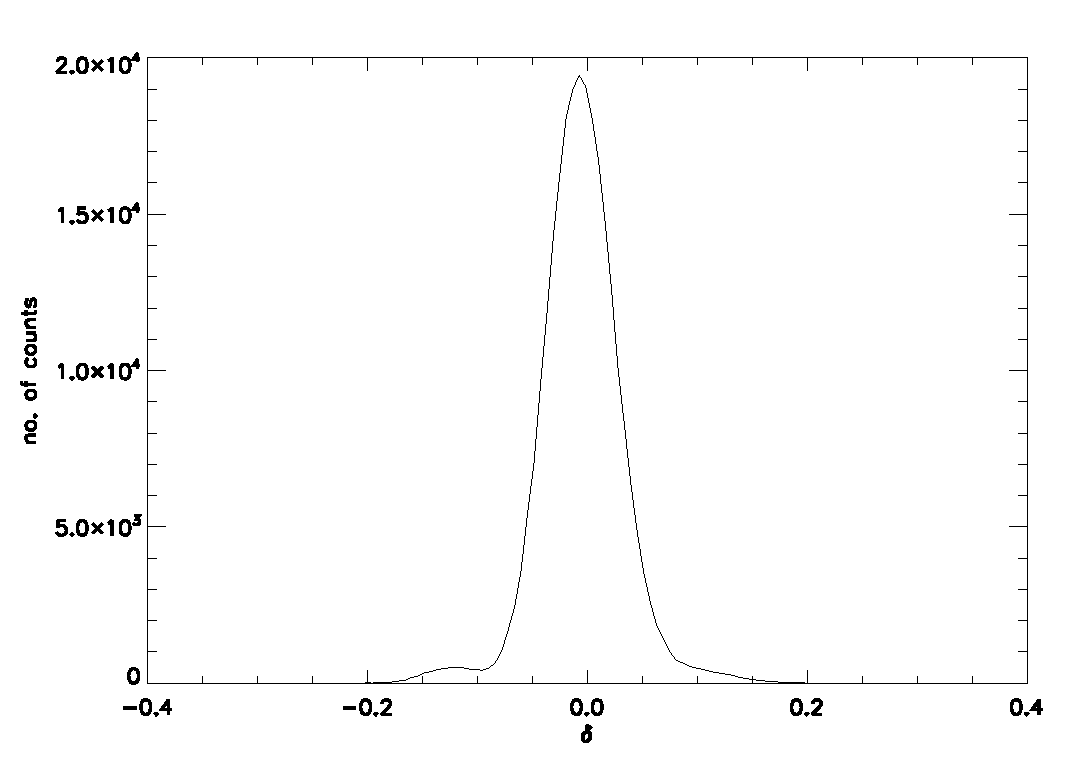
\includegraphics[width=0.49\columnwidth]{./full/wm64/hist/old/psi_r0_hist_dc}
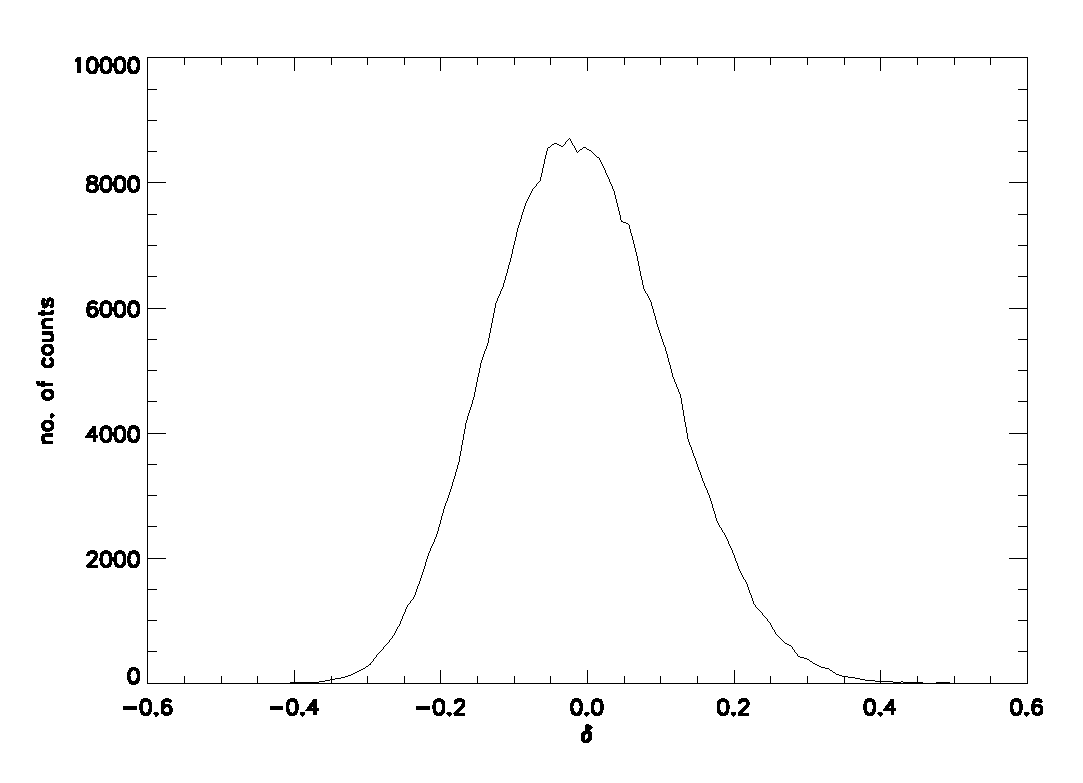
\includegraphics[width=0.49\columnwidth]{./full/wm64/hist/old/psi_r10_hist_dc}
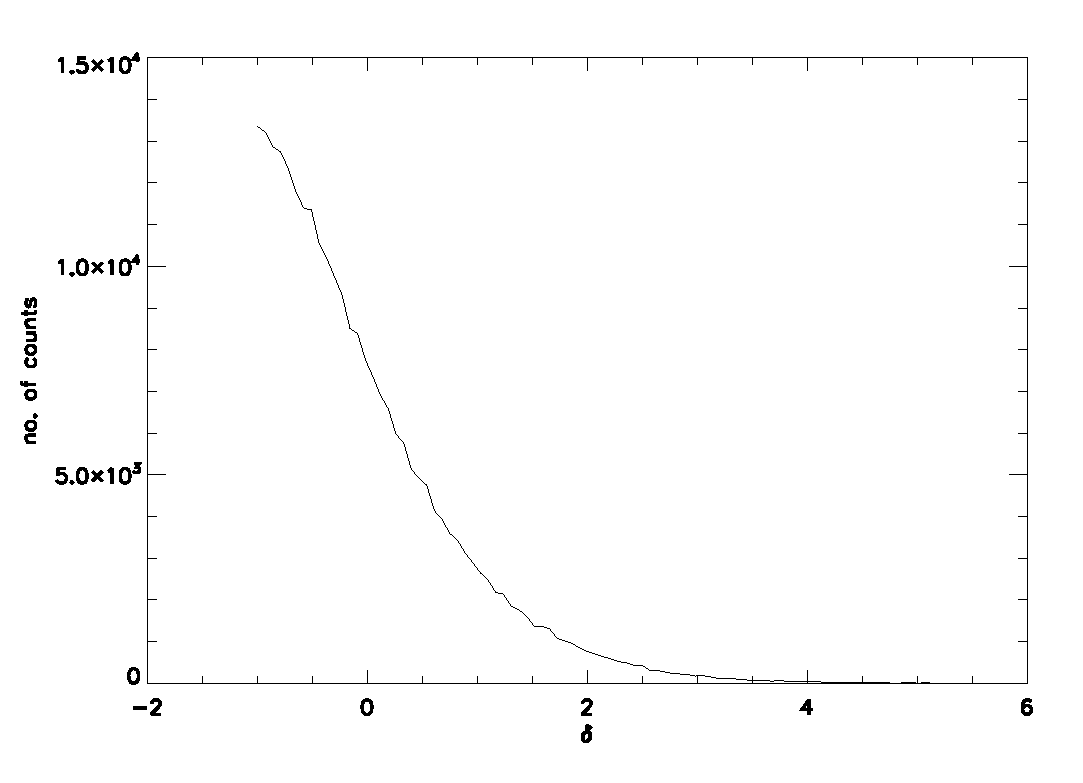
\includegraphics[width=0.49\columnwidth]{./full/wm64/hist/old/psi_r100_hist_dc}
   \end{center}
\caption{These plots show histograms of over-density as generated from the wave-mechanics code. The outputs are for timesteps = 0, 10, 100. This corresponds to $a = 0.03125, 0.0315, 0.0345$. The maximum over-density in the final plot $\delta \sim 6$ is much higher than is expected from present structure formation theory.}
\label{fig.dc_problem}
\end{figure}

Simulations of higher resolution (such as $128^3$) do not seem to suffer from the same problem: the increase in $\delta_{max}$ is more gradual. This suggests that resolutions of $64^3$ and below are just too rough for our implementation of wave-mechanics; however, we believe this problem can be resolved. We suspect the problem is to do with the initial density field generated by the TSC routine. If we take an initial field and decrease the initial magnitude of $\delta$ such that the new field is $\delta' = \delta / 10$ then the increase in the over-density is more gradual (as expected).

Before running the wave-mechanics simulation we checked the GADGET-2 files (initial and late times) to see if they were what we expected (that is, the results produce the behaviour we expected). One such test is to create histograms of the density ($\rho$) and the over-density ($\delta$) fields. The histogram of density should be gaussian in shape and show an increase in width over time. The highest density reached in each output is higher than the previous output, indicating that dense regions are accreting more material and collapsing under the force of gravity. The under dense regions are losing more mass over time (the material is attracted away from these regions in the higher density regions), hence the troughs of the density are lower with each output. The histogram at later times are also gaussian. They are plotted in figure \ref{fig.gadhist} and come from a $64^3$ simulation.

The behaviour of the over-density fields (from GADGET-2) corroborates with the behaviour of the density field. The histogram of over-density is initially gaussian but tends towards a log-normal in later outputs as seen in figure \ref{fig.gadhistdc}. The initial density field is smooth where deviations from the mean density are small, as indicated by the tight distribution in the first histogram of over-density (a standard deviation of about 0.02). The over-density field is skewed as the minimum value (by definition) is -1 while the maximum can increase (almost) without bound.

\begin{figure}[htb]
   \begin{center}
     %\leavevmode..

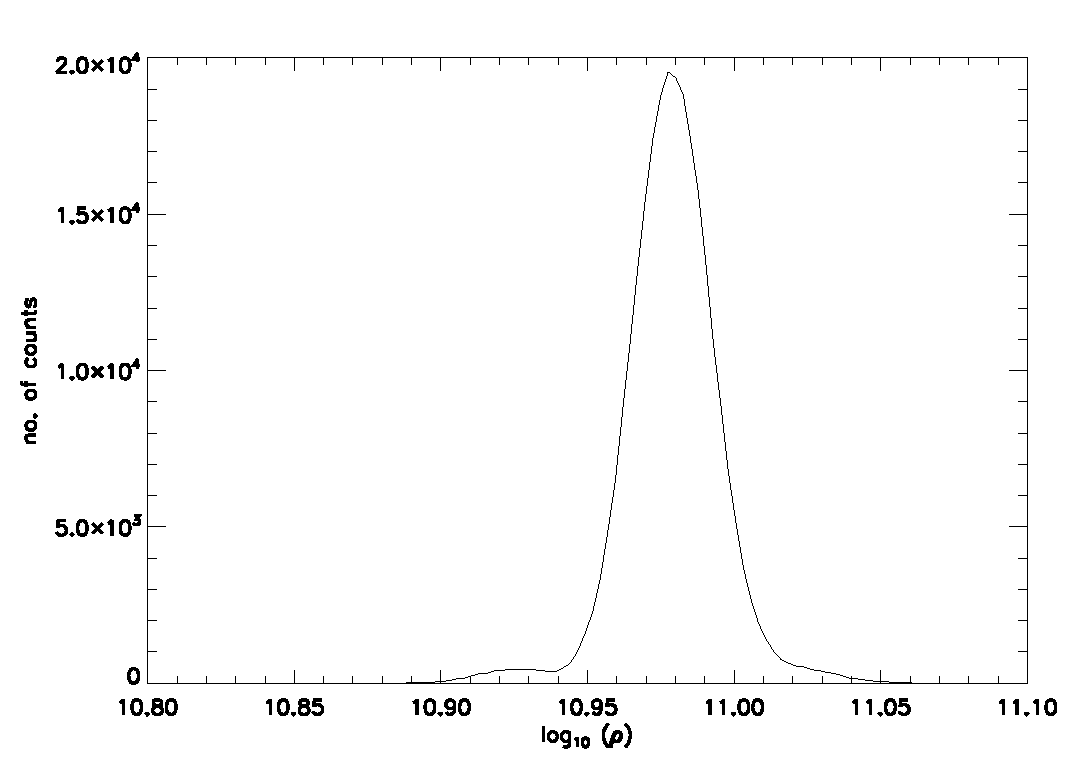
\includegraphics[width=0.49\columnwidth]{./full/gadget/hist_0000}
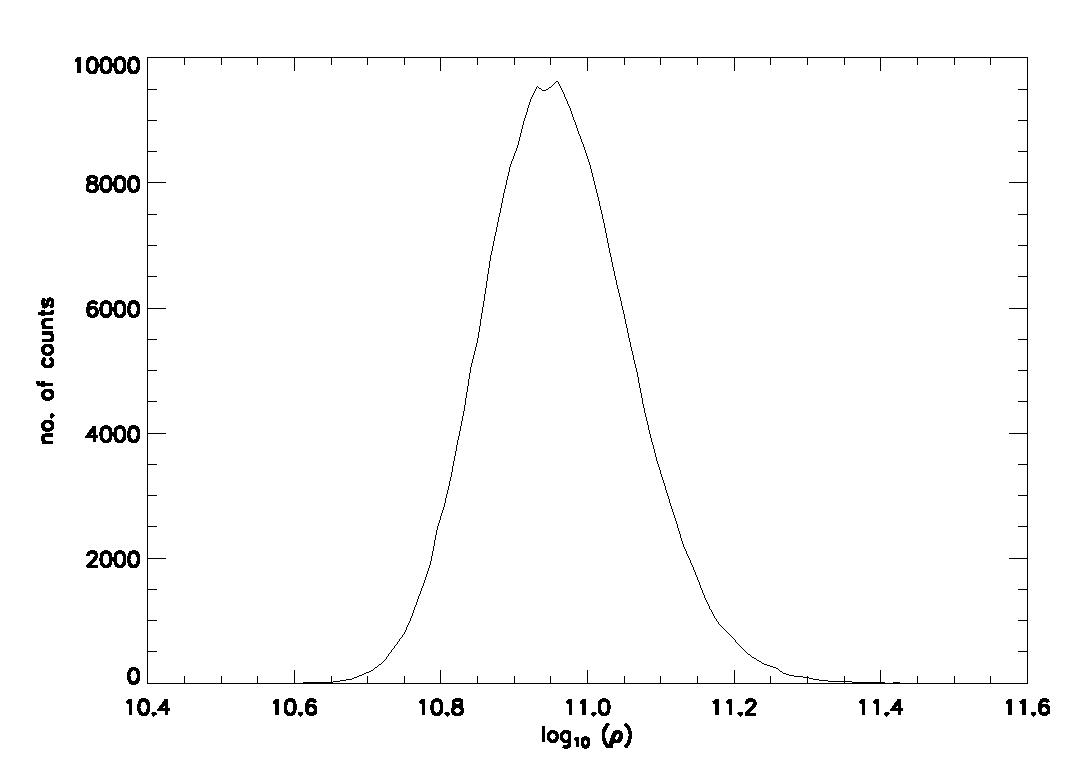
\includegraphics[width=0.49\columnwidth]{./full/gadget/hist_000}
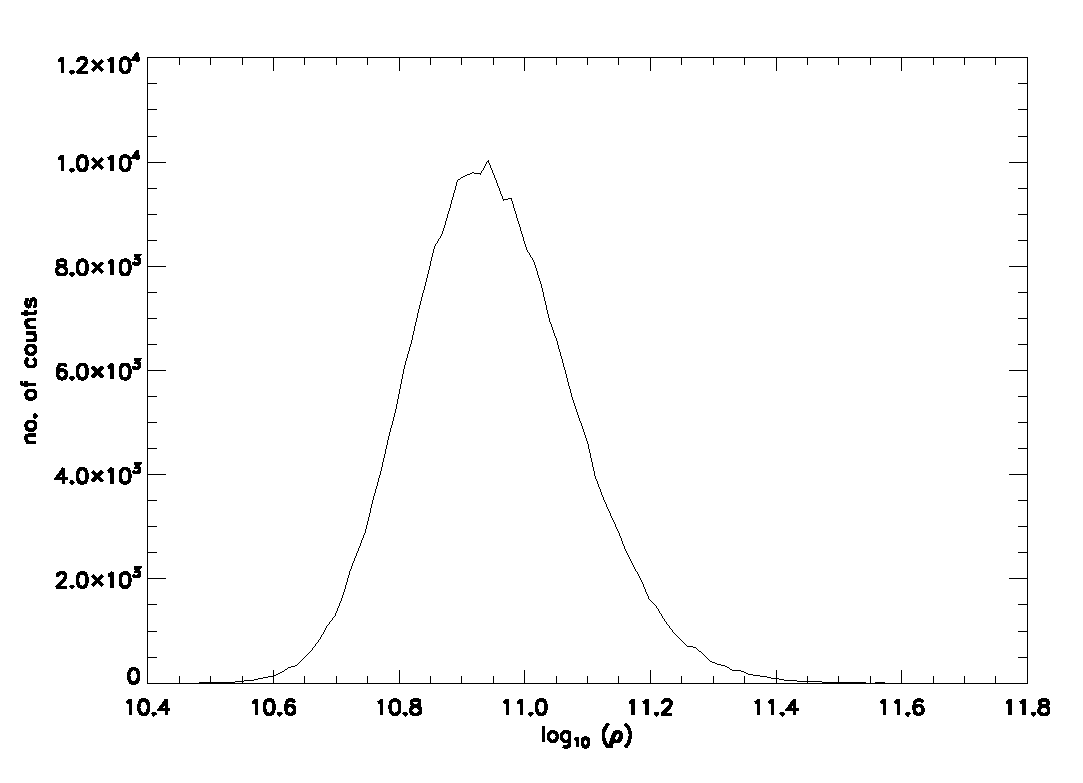
\includegraphics[width=0.49\columnwidth]{./full/gadget/hist_001}
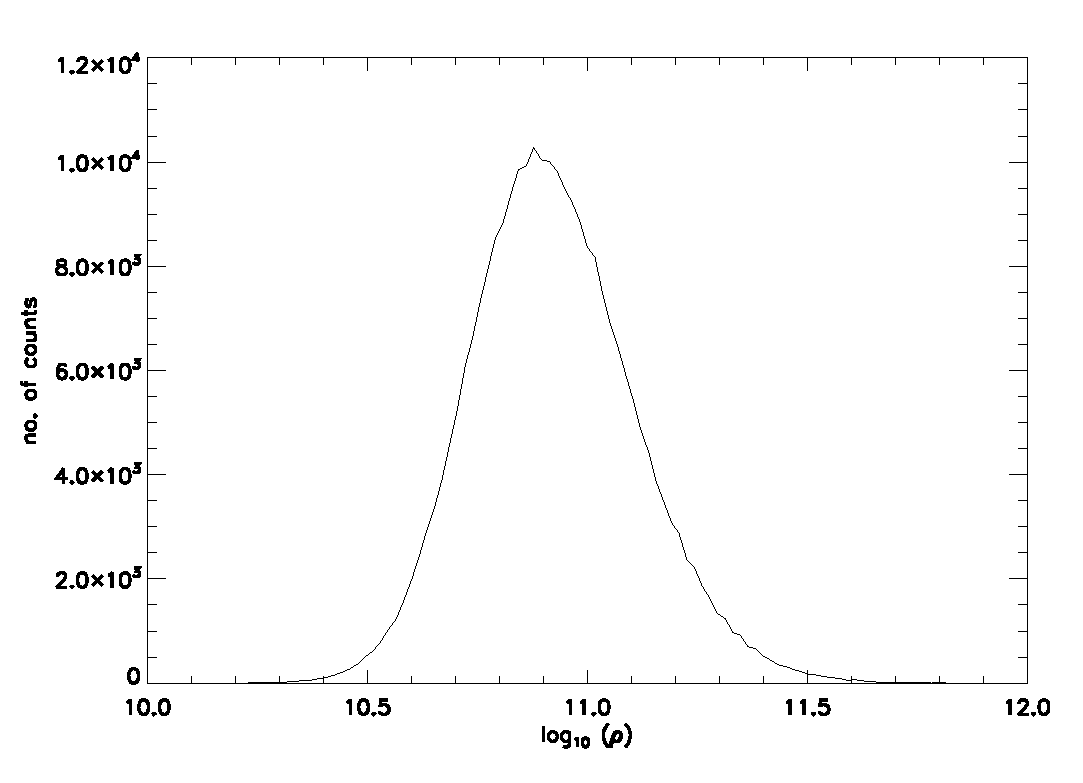
\includegraphics[width=0.49\columnwidth]{./full/gadget/hist_002}
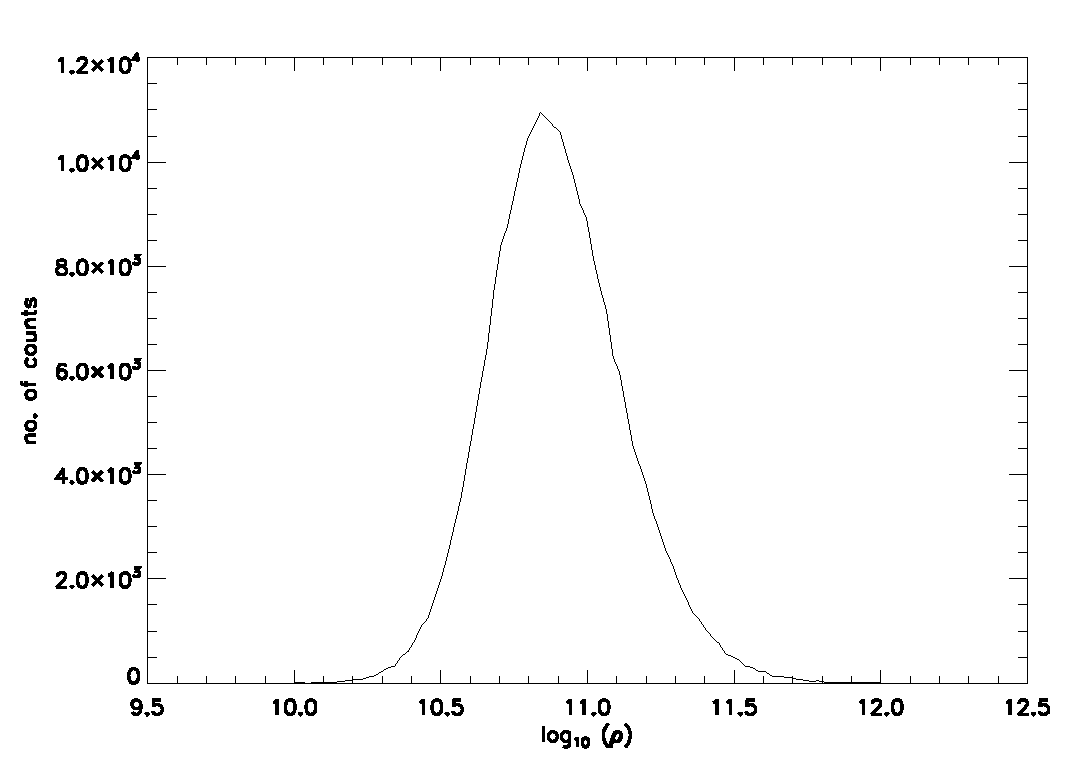
\includegraphics[width=0.49\columnwidth]{./full/gadget/hist_003}
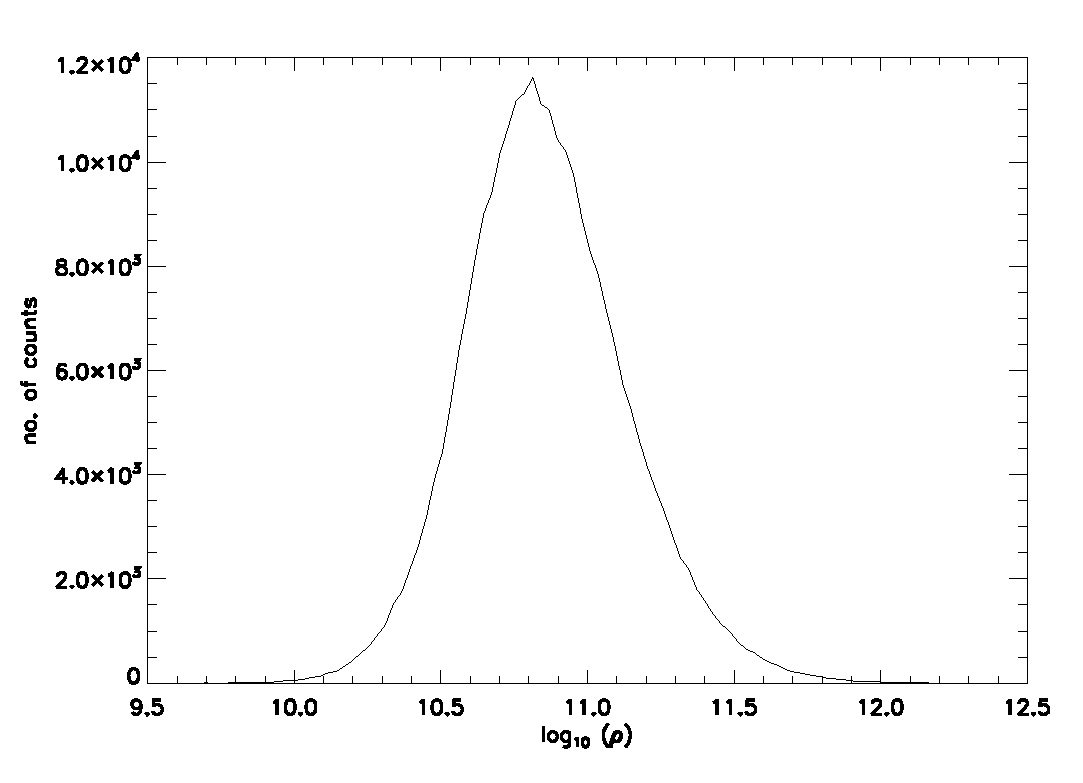
\includegraphics[width=0.49\columnwidth]{./full/gadget/hist_004}

   \end{center}
\caption{These plots show histograms of density as generated from the GADGET-2 outputs. They have a distinctly gaussian shape and widen over time. The outputs are for $z = 32, 3, 2, 1, 0.5, 0.05.$}
\label{fig.gadhist}
\end{figure}

\begin{figure}[htb]
   \begin{center}
    % \leavevmode

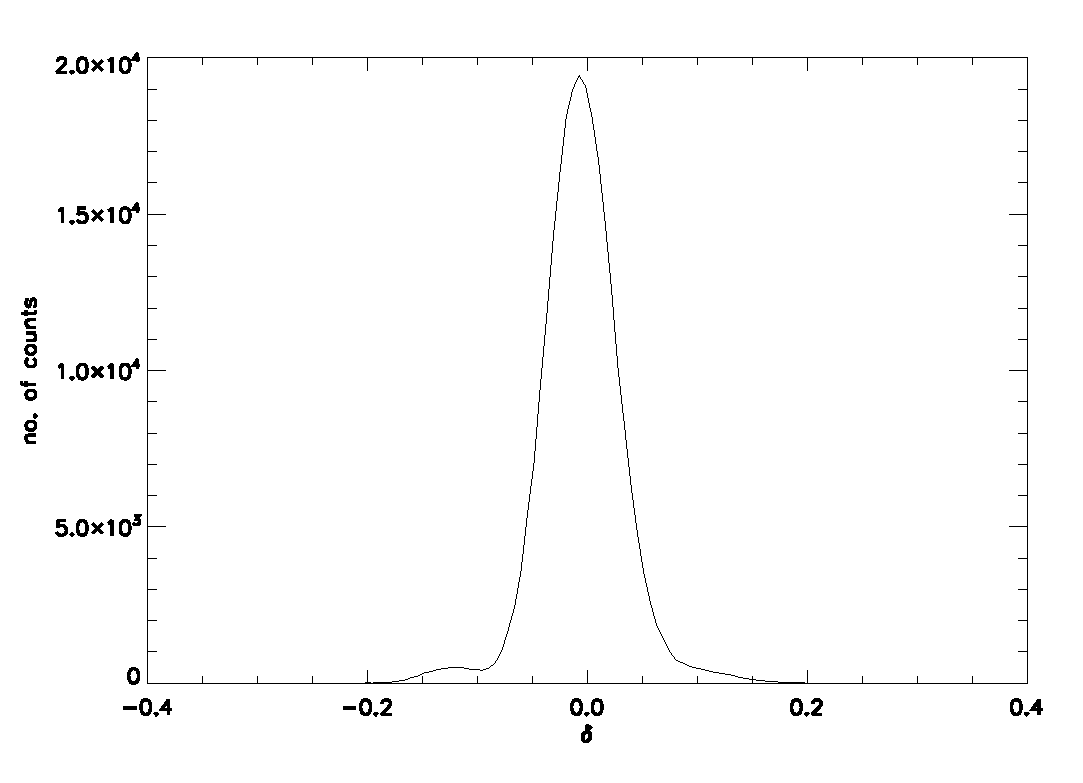
\includegraphics[width=0.49\columnwidth]{./full/gadget/hist_delta_0000}
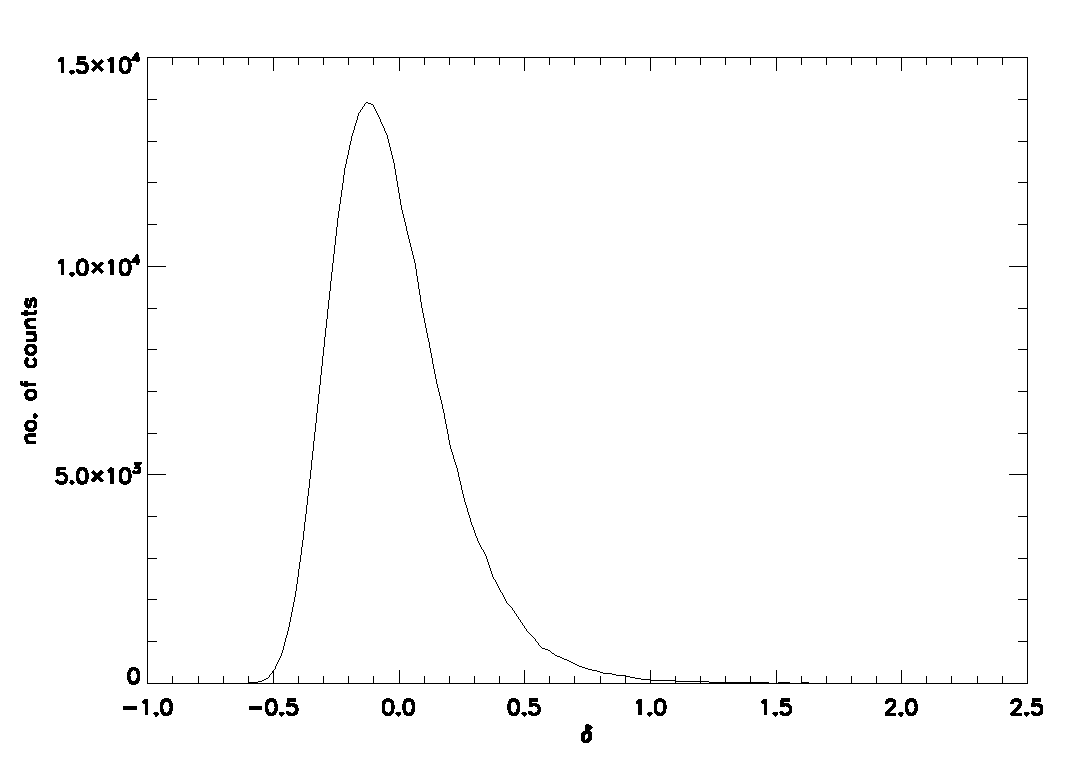
\includegraphics[width=0.49\columnwidth]{./full/gadget/hist_delta_000}
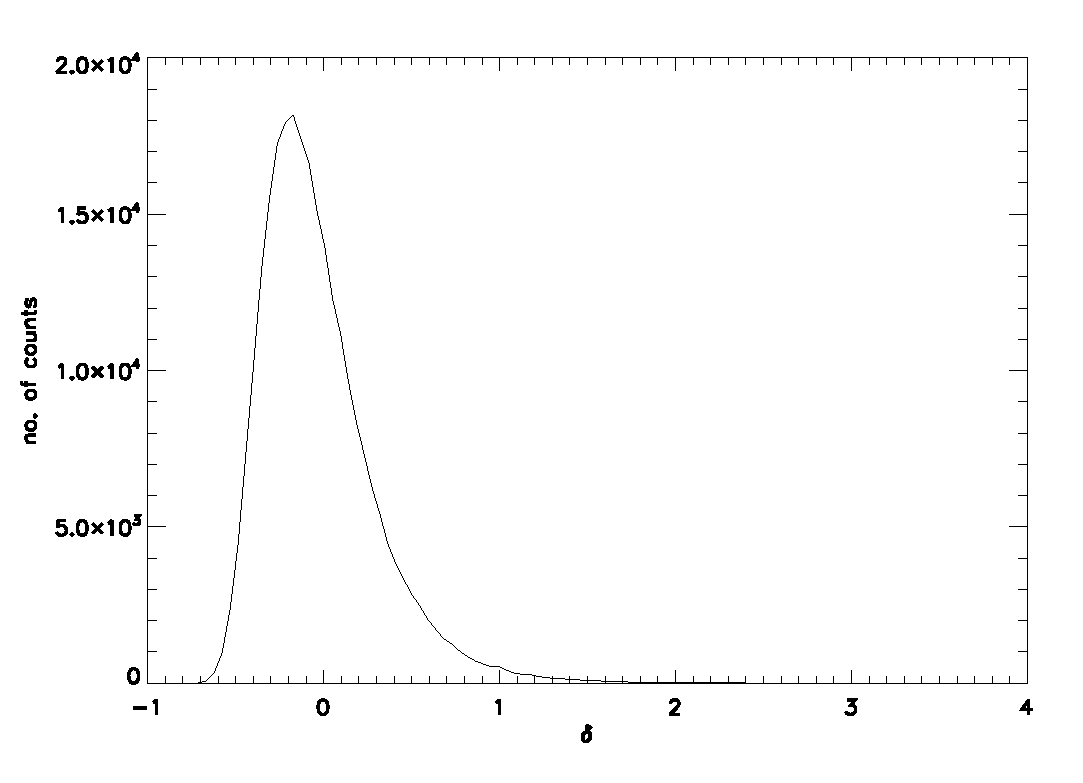
\includegraphics[width=0.49\columnwidth]{./full/gadget/hist_delta_001}
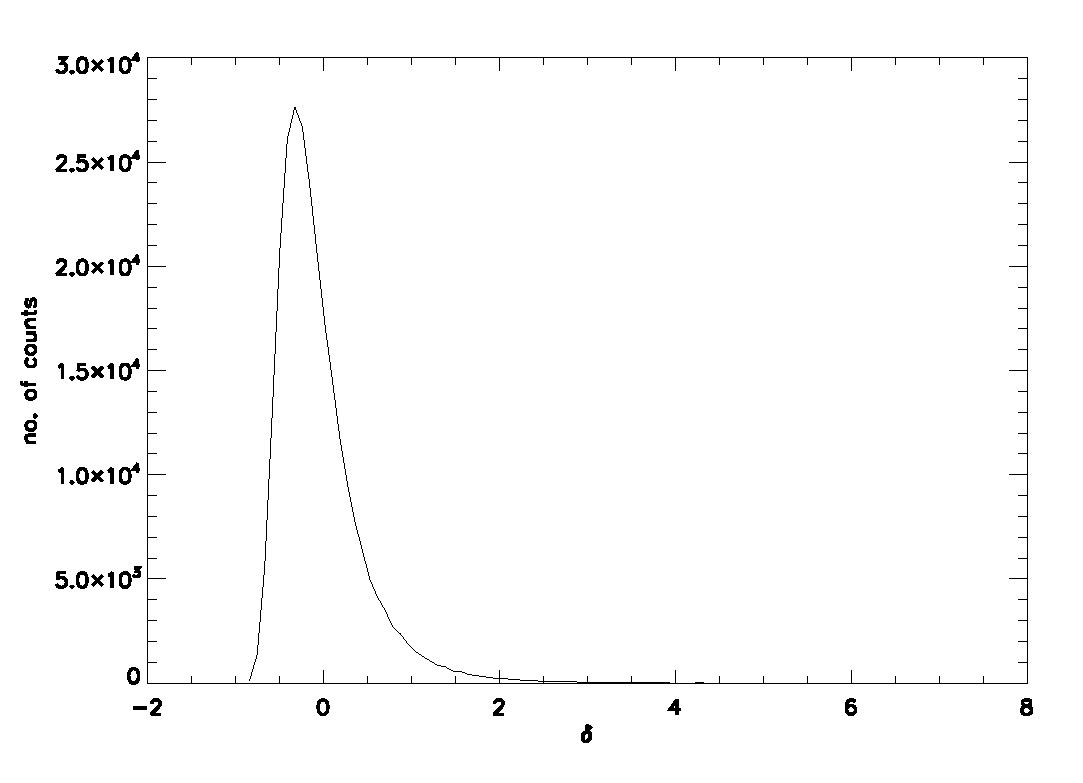
\includegraphics[width=0.49\columnwidth]{./full/gadget/hist_delta_002}
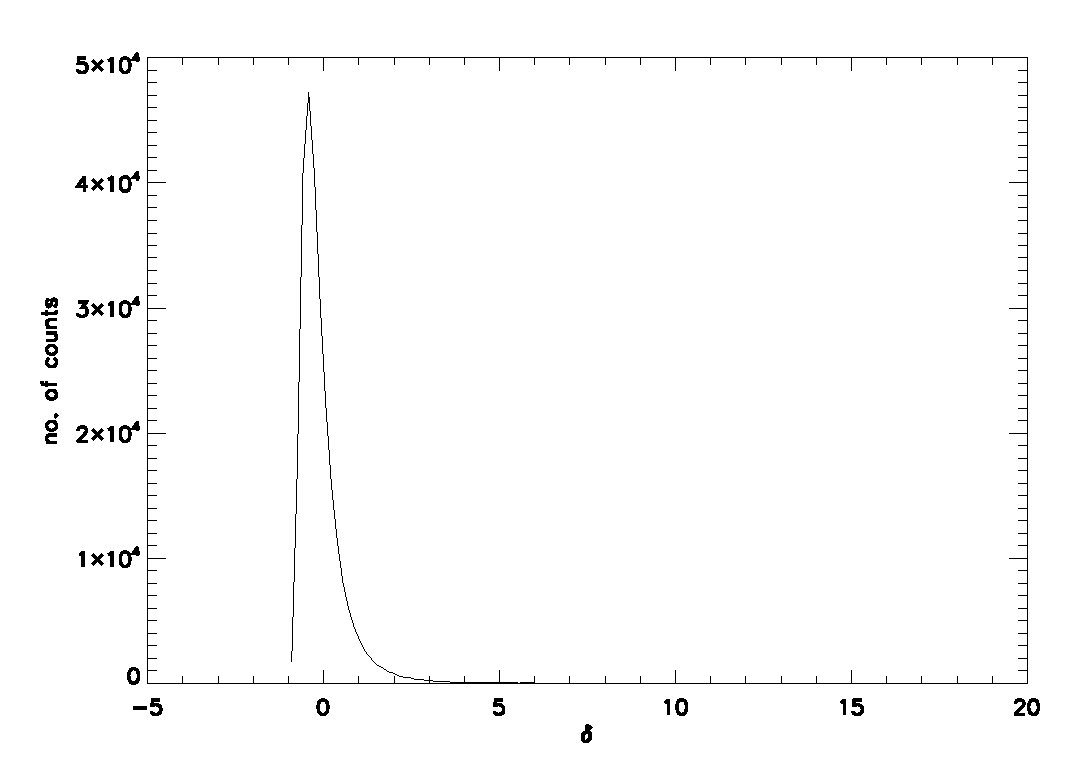
\includegraphics[width=0.49\columnwidth]{./full/gadget/hist_delta_003}
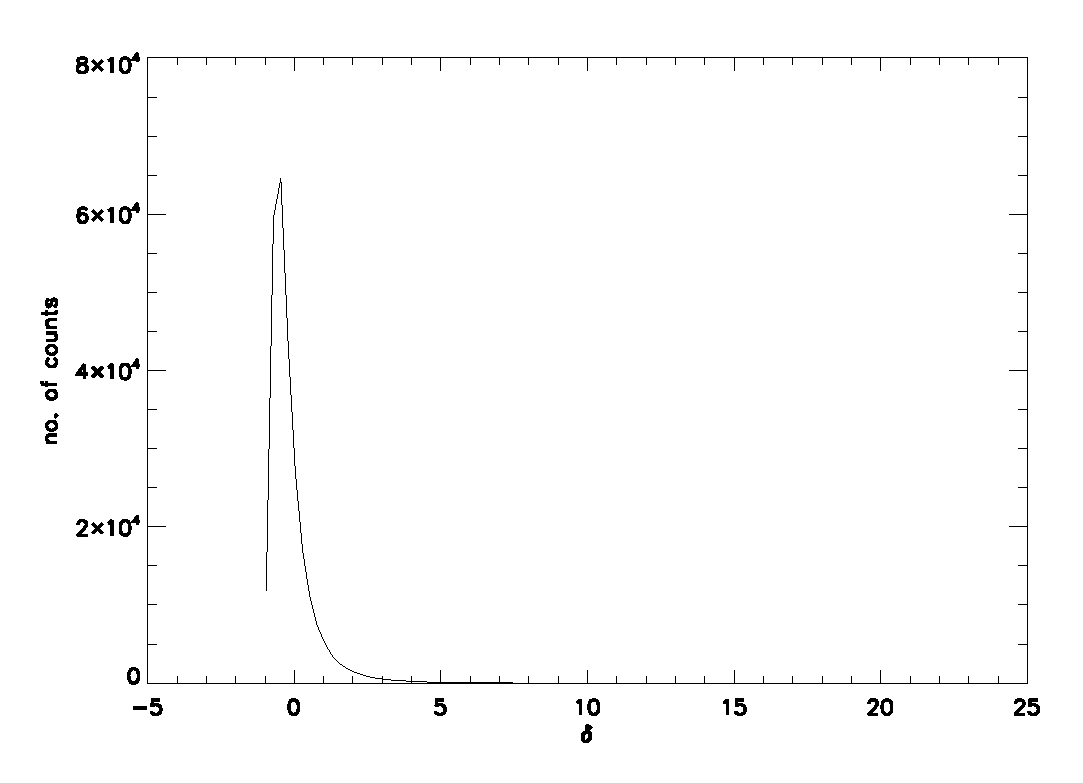
\includegraphics[width=0.49\columnwidth]{./full/gadget/hist_delta_004}

   \end{center}
\caption{These plots show histograms of over-density as generated from the GADGET-2 outputs. The outputs are for $z = 32, 3, 2, 1, 0.5, 0.05.$}
\label{fig.gadhistdc}
\end{figure}

% check velocities are maxwellian?
The evolution of density and over-density from the wave-mechanics code is similar to that of GADGET-2 but not the same. The initial conditions are the same, as required. However, in the wave-mechanics outputs (see figure \ref{fig.wmhist}), the gaussian shape of the density field skews over time with the peak leaning towards the higher mass end. It also develops a long tail, to balance the skewing towards the top end, as the under-dense regions evacuate. The highest peak of density (and over-density) never goes as high as it does in the GADGET-2 outputs. However, the lowest trough of density is far lower than that of GADGET-2: $\rho_{min} \sim 10^6$ for wave-mechanics while GADGET-2 only goes as low as $\rho_{min} \sim 10^{9.5}$. The under-dense regions are evacuated faster in wave-mechanics, hence the over-density histogram (figure \ref{fig.wmhistdc}) approaches a log-normal shape more rapidly than it does for GADGET-2. This was not expected and may be a characteristic feature of wave-mechanics, though an implementation-dependent cause cannot be ruled out. All resolutions and choice of $\nu$ tested seem to produce similar behaviour, the results shown in figure \ref{fig.wmhistdc} are typical plots.

A further unexpected outcome of wave-mechanics is the rapid variability in the height of density ($\rho$) from gridpoint to gridpoint (see figure \ref{fig.wmrho}). Naturally, the GADGET-2 outputs can be expected to be smoother as they density field is not continuous but rather is calculated from the discrete distribution of particles. The wave-mechanics code gives more lows and more highs (by number count) than GADGET-2, while the lowest trough and highest peak are lower than that of GADGET-2. Again, this appears to be true regardless of resolution.

The plots in figure \ref{fig.wmrho} have a resolution of $64^3$ with $\nu = 10^{-7}$ and $|\delta|_{\rm initial} \sim 0.03$, otherwise all initial conditions are the same as for the GADGET-2 simulation. In figure \ref{fig.dc_problem}, we noted there was a problem with the maximum value of $\delta$ being too large. There, $\delta_{max} = 6$ after 100 timesteps when $|\delta|_{\rm initial} \sim 0.3$. In the latest run where $|\delta|_{\rm initial} \sim 0.03$, the $\delta_{max}$ from this simulation after 100 timesteps run was $\delta_{max} = 0.7$. This is of a more acceptable magnitude.

In addition to the histograms (\ref{fig.wmhist}, \ref{fig.wmhistdc}) and the surface plots of density (\ref{fig.wmrho}), I provide a contour plot of over-density (figure \ref{fig.delta_contour}) which has levels at $\delta =  -1, 0, 1, 2, 5$. From the surface plots (\ref{fig.wmrho}) it is hard, at first, to tell if the structure is random as it appears to rapidly change from timestep to timestep. The data is messier than from GADGET-2, so the conclusion is not as immediately obvious. The contour plots give the clearest picture of how the structure is fragmentary but not completely random. Implicitly, the data has been smoothed to hide the finest structure.

A possible source of such messiness is due to the fact that the whole simulation uses a single coherent wavefunction. As shown in the results of section \ref{per_bou}, a single wavefunction can lead to interference effects. Although we hope to limit this effect by using a small $\nu$ we may not have completely suppressed these effects. That is despite the fact gravity also acts to suppress such interference effects.

In contrast to the GADGET-2 density, the plots of wave-mechanics show more structure. For comparison we can look at the contour plots generated for GADGET-2 (figure \ref{fig.gadget_contour}). These latter plots are far smoother than that of wave-mechanics. It seems also impossible to tell that the results of wave-mechanics and GADGET-2 come from the same initial conditions. It should be noted that the highest value of $\delta$ for GADGET-2 was $\delta \sim 23$, which is far higher than that of wave-mechanics $\delta \sim 9 \rightarrow 14$ (depending on parameter choice: such as varying $\nu$).


All of the following outputs are shown for timesteps: $0, 200, 1000, 2000, 3000, 3500$, or $a = 0.03125,0.038,0.085,0.23, 0.63, 1.03$. The slices through the data were all taken at the some point on the z-axis: $L/2$.


\begin{figure}[htb]
   \begin{center}
     %\leavevmode

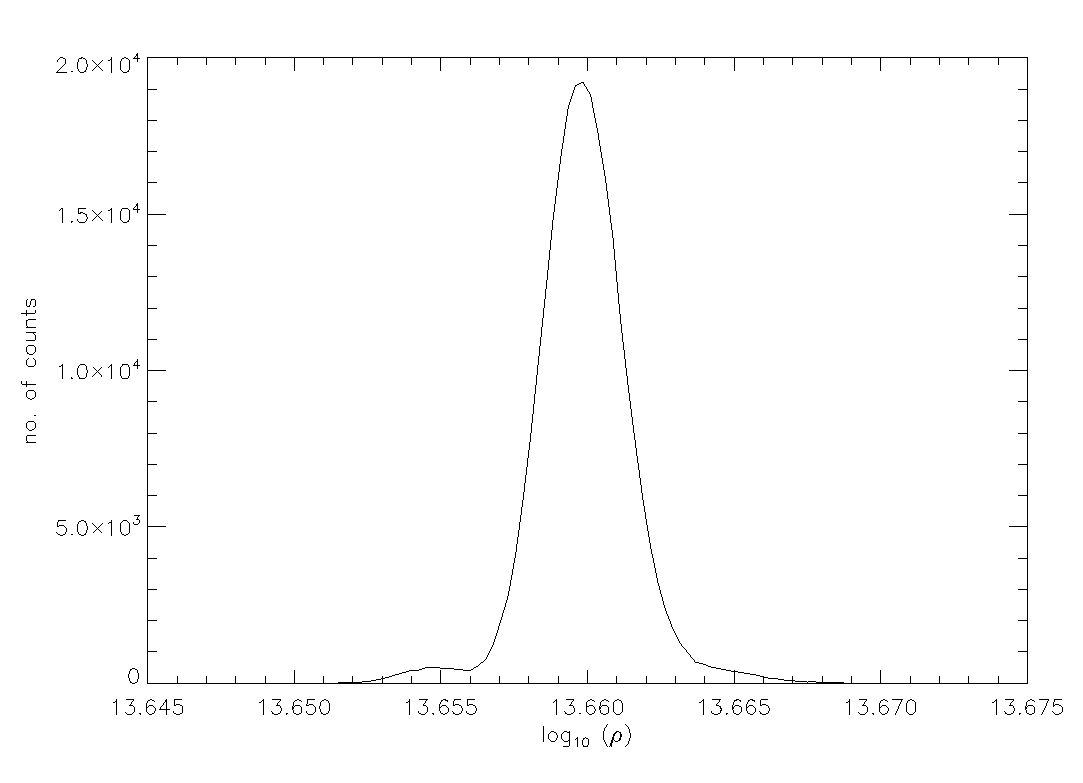
\includegraphics[width=0.49\columnwidth]{./full/wm64/hist/r00000_hist}
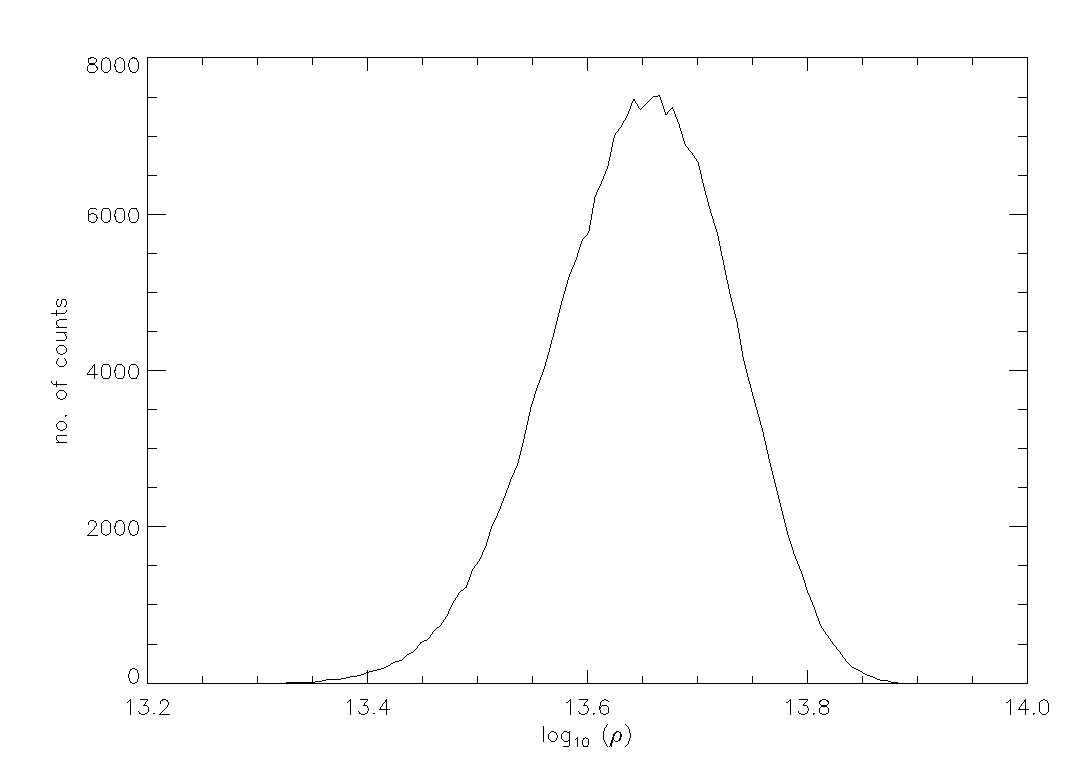
\includegraphics[width=0.49\columnwidth]{./full/wm64/hist/r00200_hist}
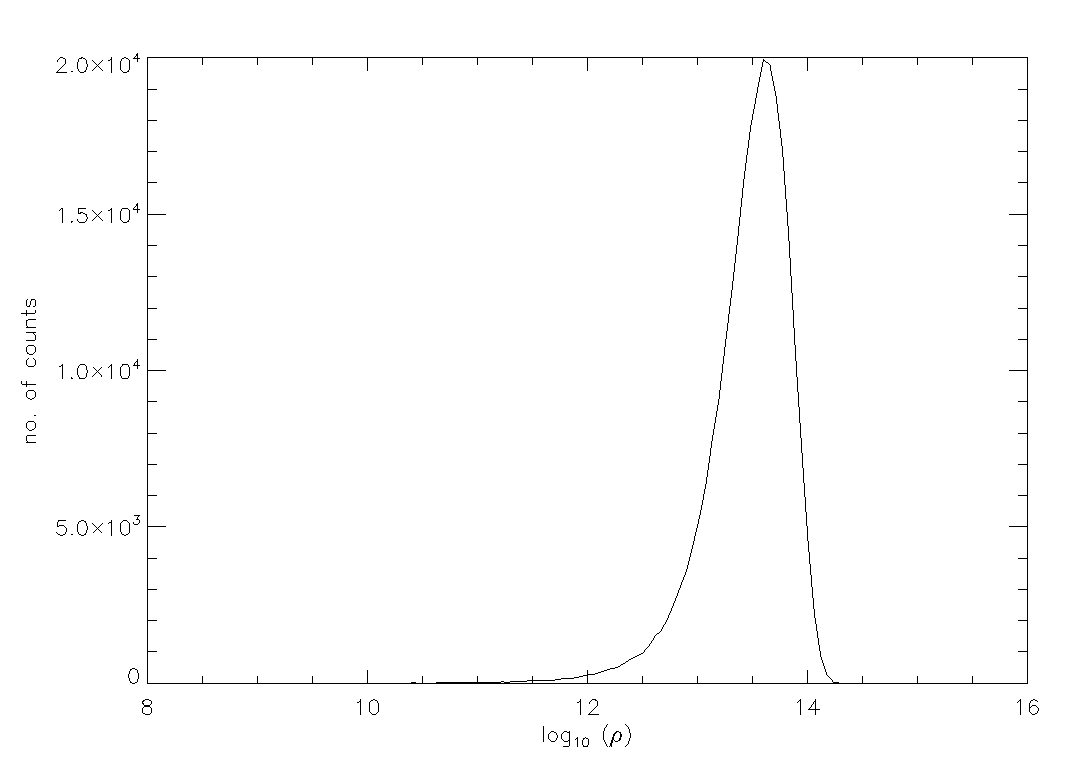
\includegraphics[width=0.49\columnwidth]{./full/wm64/hist/r01000_hist}
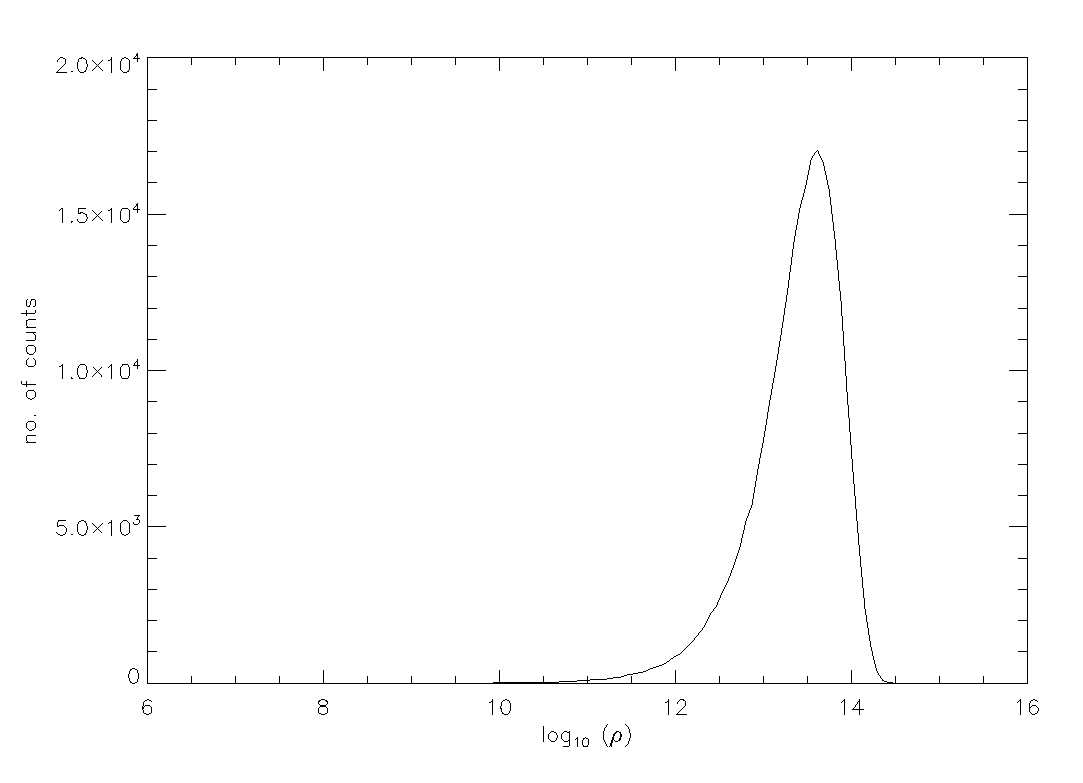
\includegraphics[width=0.49\columnwidth]{./full/wm64/hist/r02000_hist}
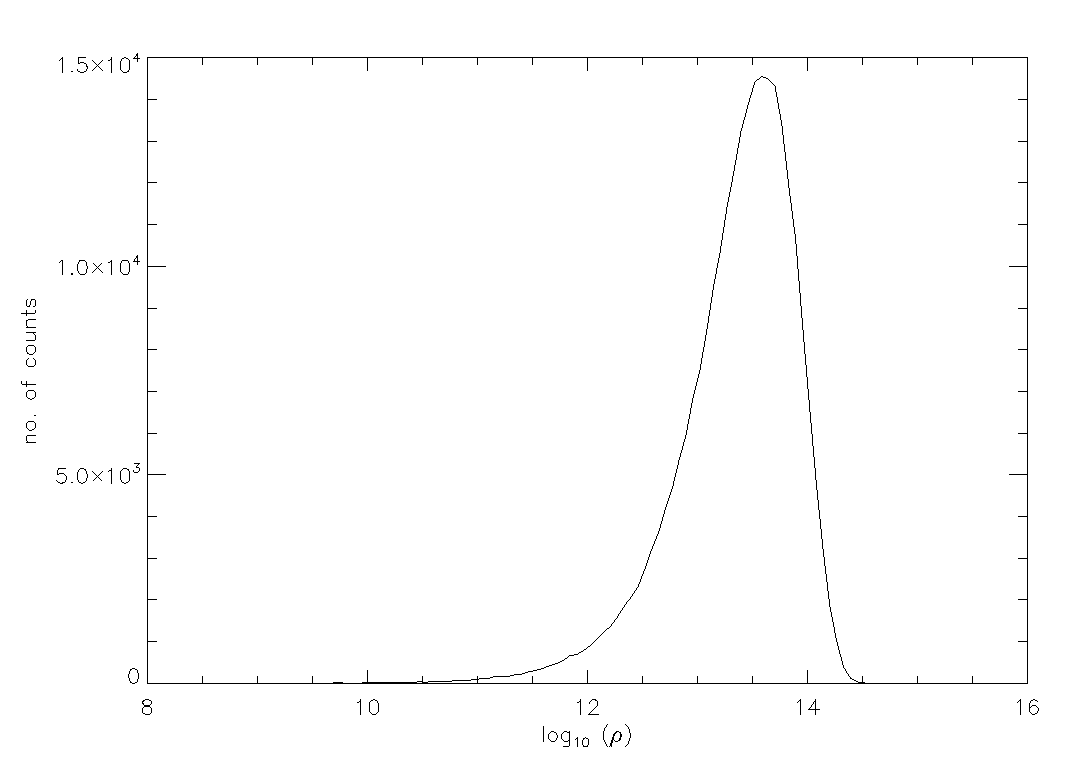
\includegraphics[width=0.49\columnwidth]{./full/wm64/hist/r03000_hist}
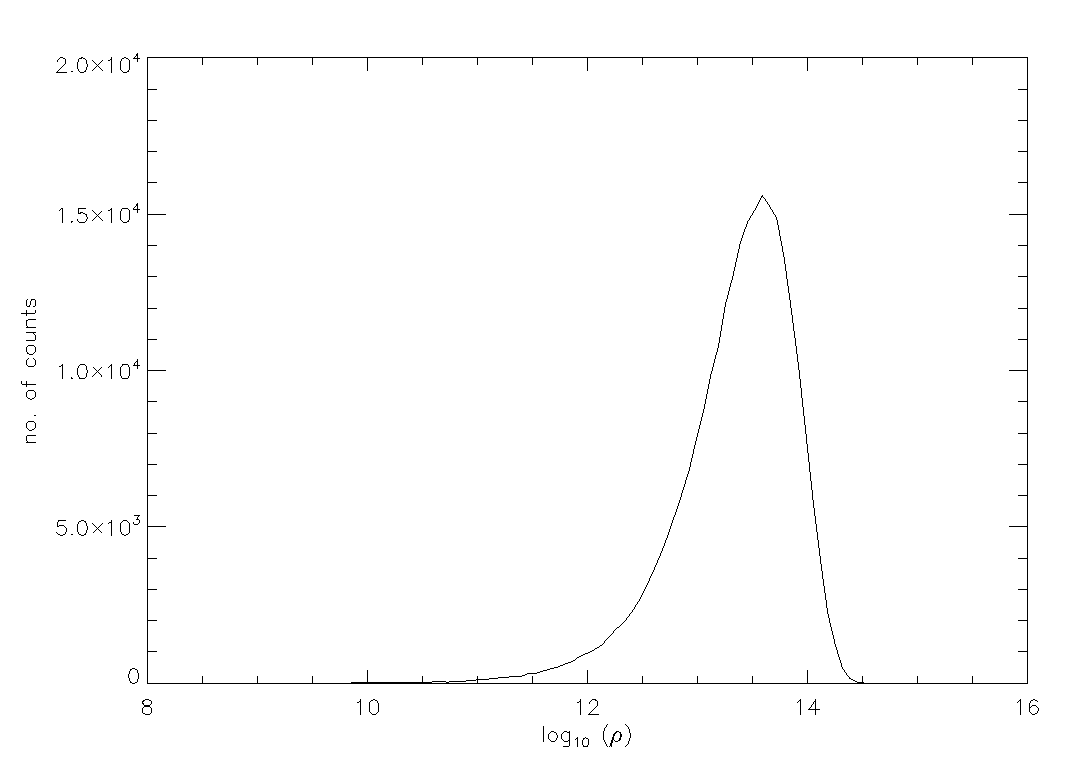
\includegraphics[width=0.49\columnwidth]{./full/wm64/hist/r03500_hist}

   \end{center}
\caption{These plots show histograms of density ($\rho$) as generated from the wave-mechanics code. They have a distinctly gaussian shape but widen and skew over time. The outputs at $t = 0, 200, 1000,$ $2000, 3000, 3500$ ($a = 0.03125,0.038,$ $0.085,0.23, 0.63, 1.03$).}
\label{fig.wmhist}
\end{figure}

\begin{figure}[htb]
   \begin{center}
     %\leavevmode

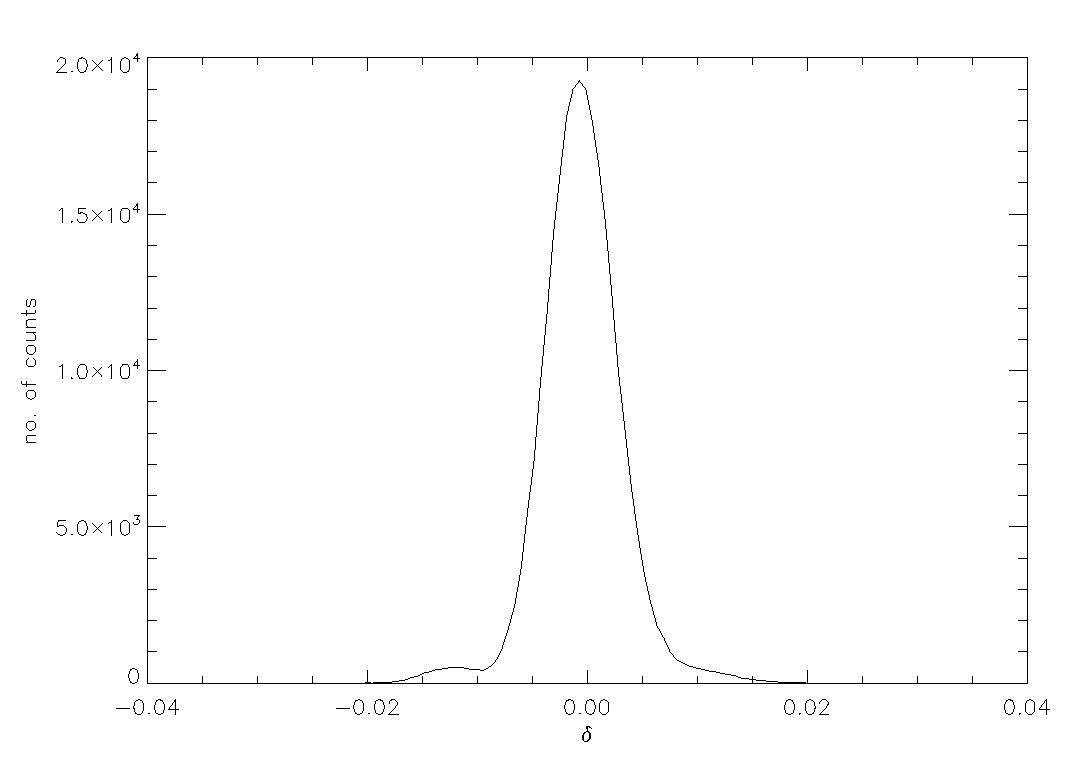
\includegraphics[width=0.49\columnwidth]{./full/wm64/hist/r00000_hist_dc}
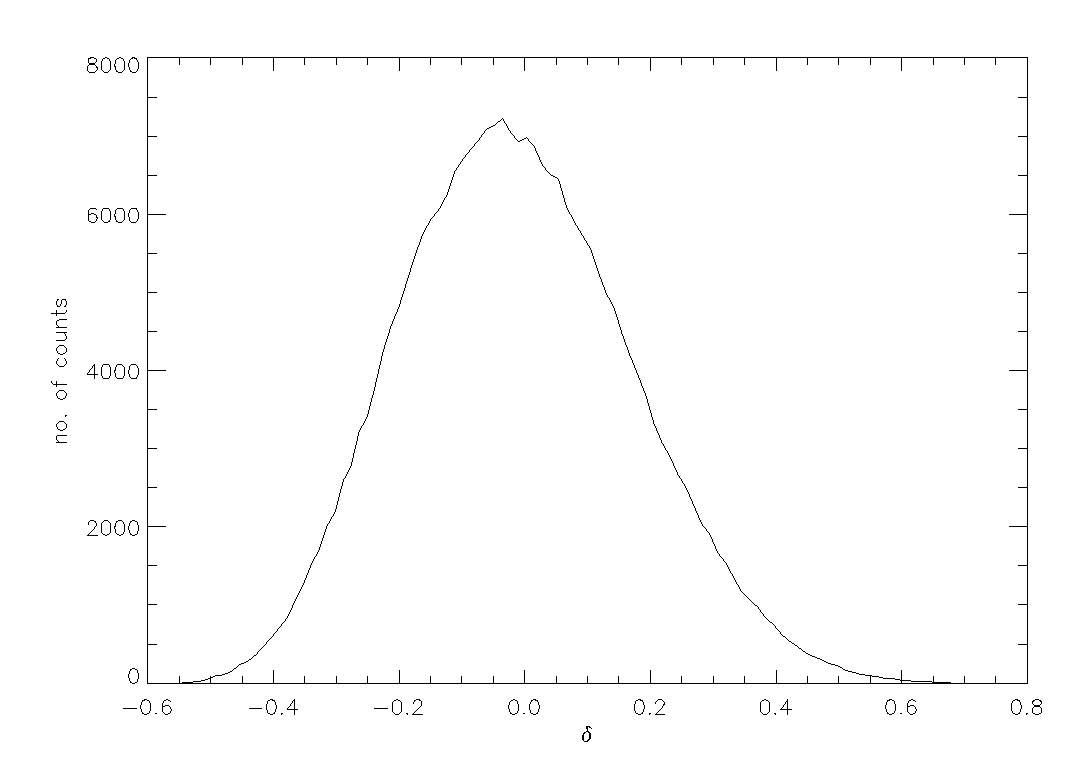
\includegraphics[width=0.49\columnwidth]{./full/wm64/hist/r00200_hist_dc}
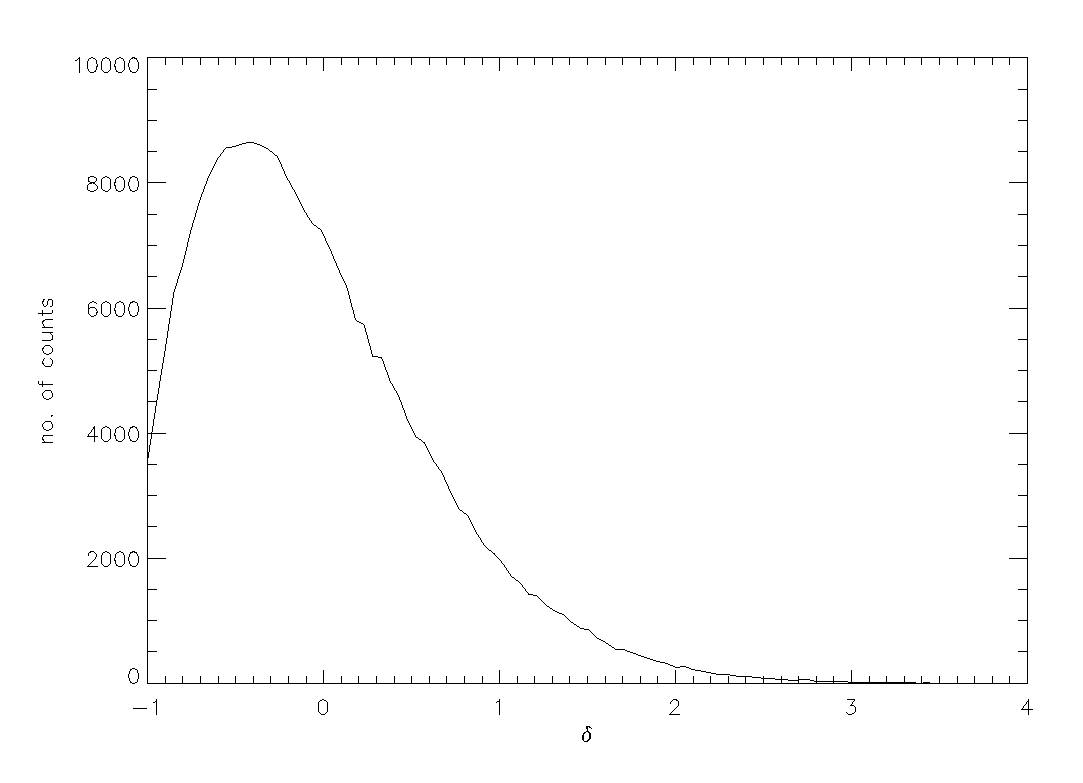
\includegraphics[width=0.49\columnwidth]{./full/wm64/hist/r01000_hist_dc}
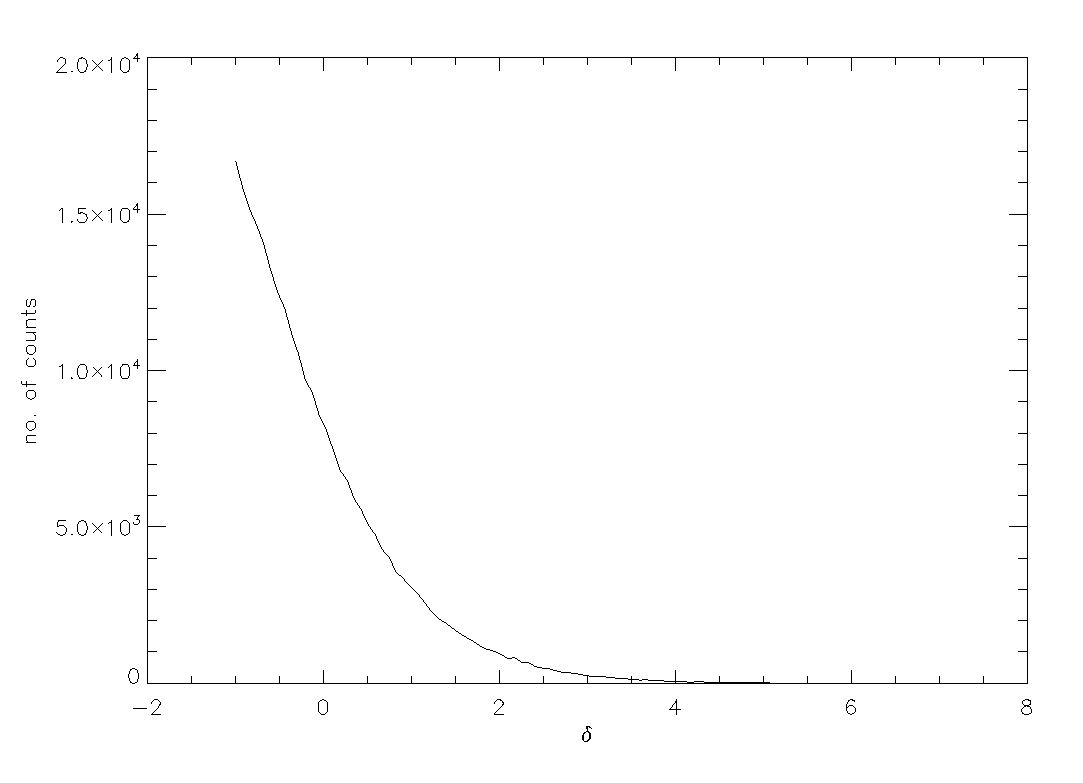
\includegraphics[width=0.49\columnwidth]{./full/wm64/hist/r02000_hist_dc}
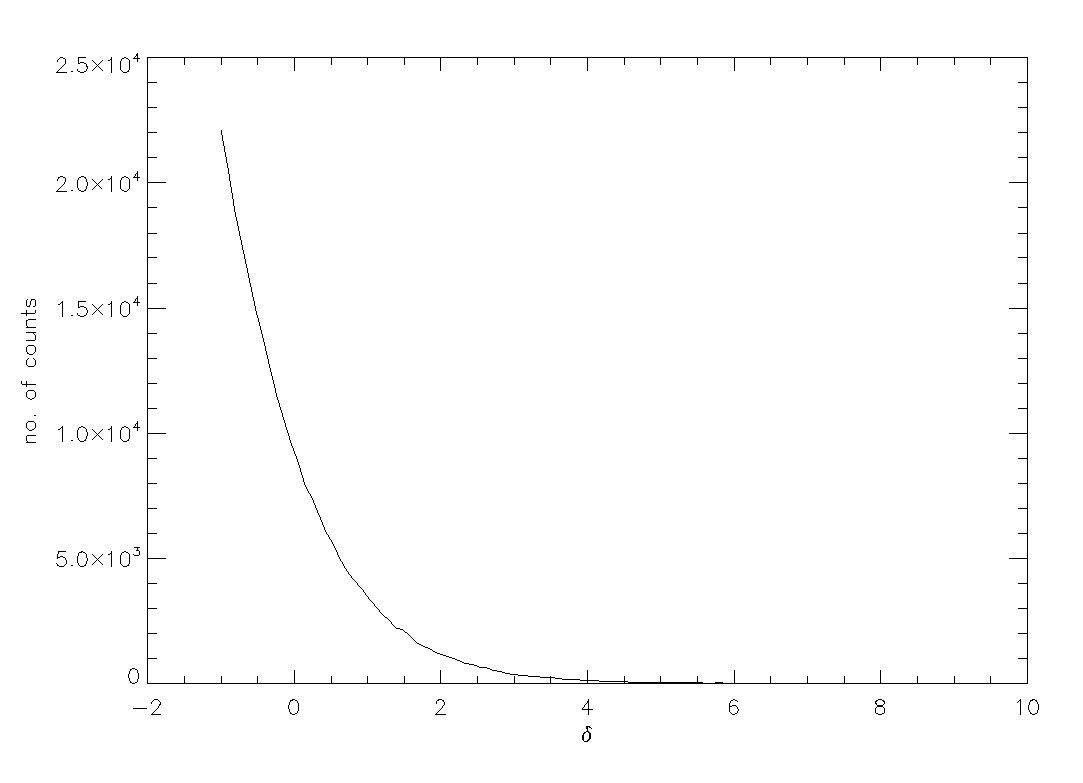
\includegraphics[width=0.49\columnwidth]{./full/wm64/hist/r03000_hist_dc}
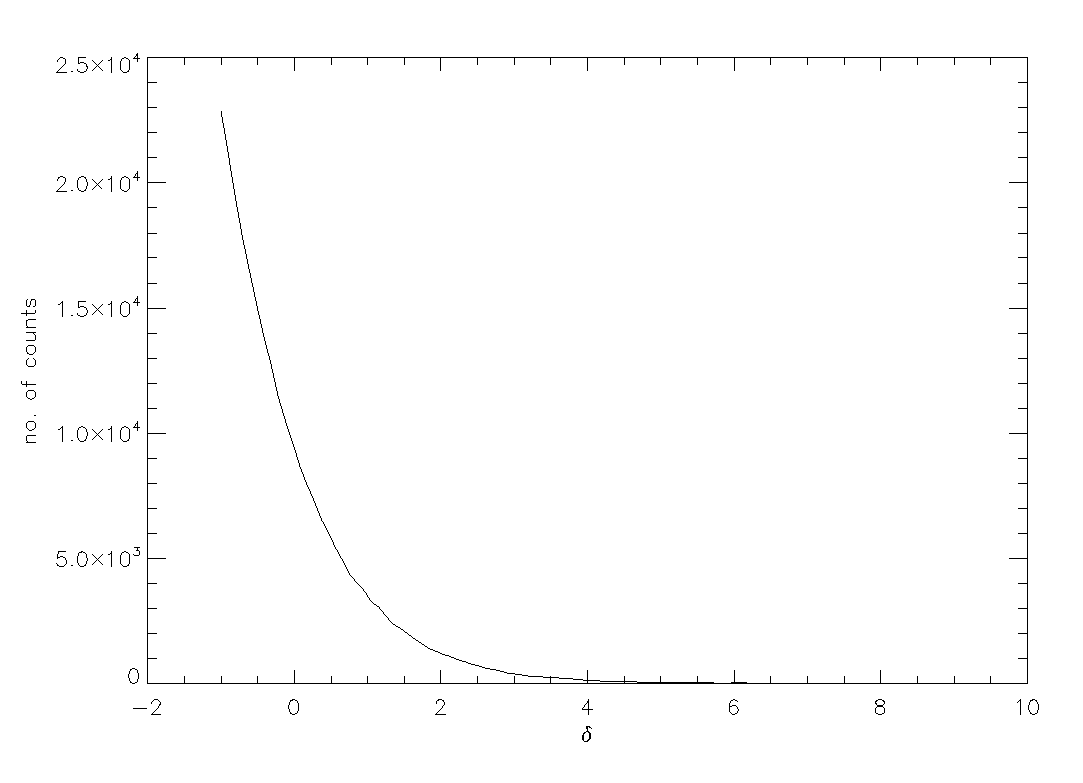
\includegraphics[width=0.49\columnwidth]{./full/wm64/hist/r03500_hist_dc}

   \end{center}
\caption{These plots show histograms of density contrast ($\delta$) as generated from the wave-mechanics code. Outputs at $t = 0, 200, 1000, 2000, 3000, 3500$.}
\label{fig.wmhistdc}
\end{figure}

\begin{figure}[htb]
   \begin{center}
     %\leavevmode

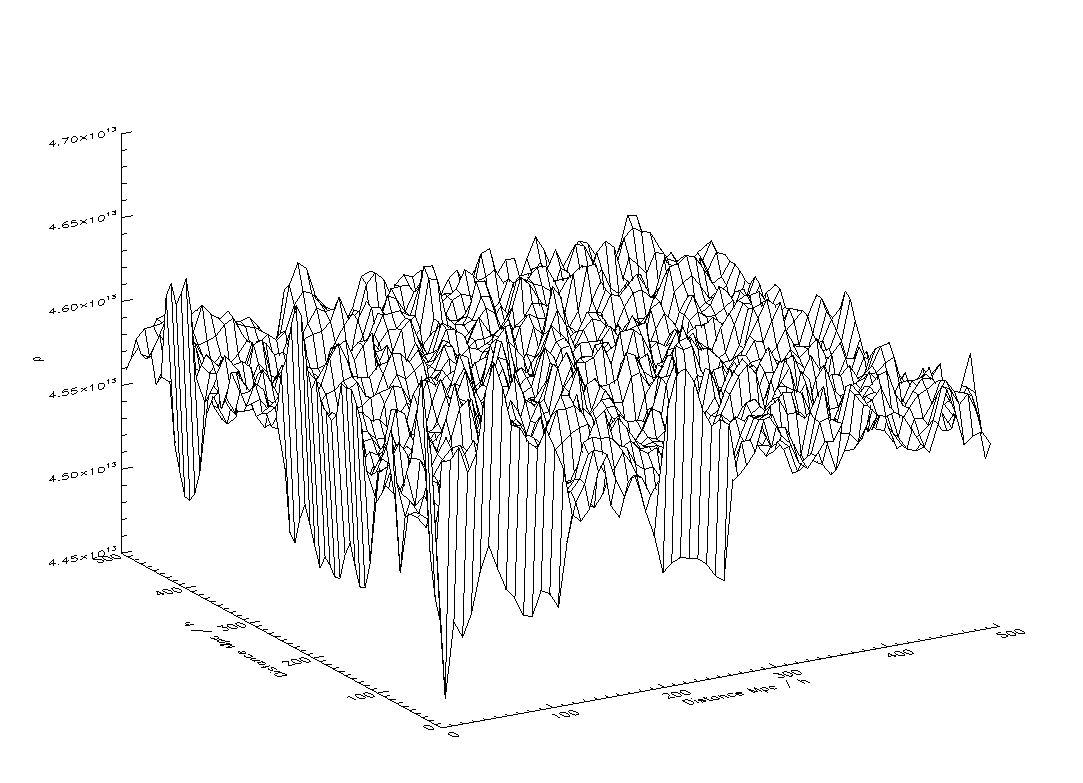
\includegraphics[width=0.49\columnwidth]{./full/wm64/rho/r00000}
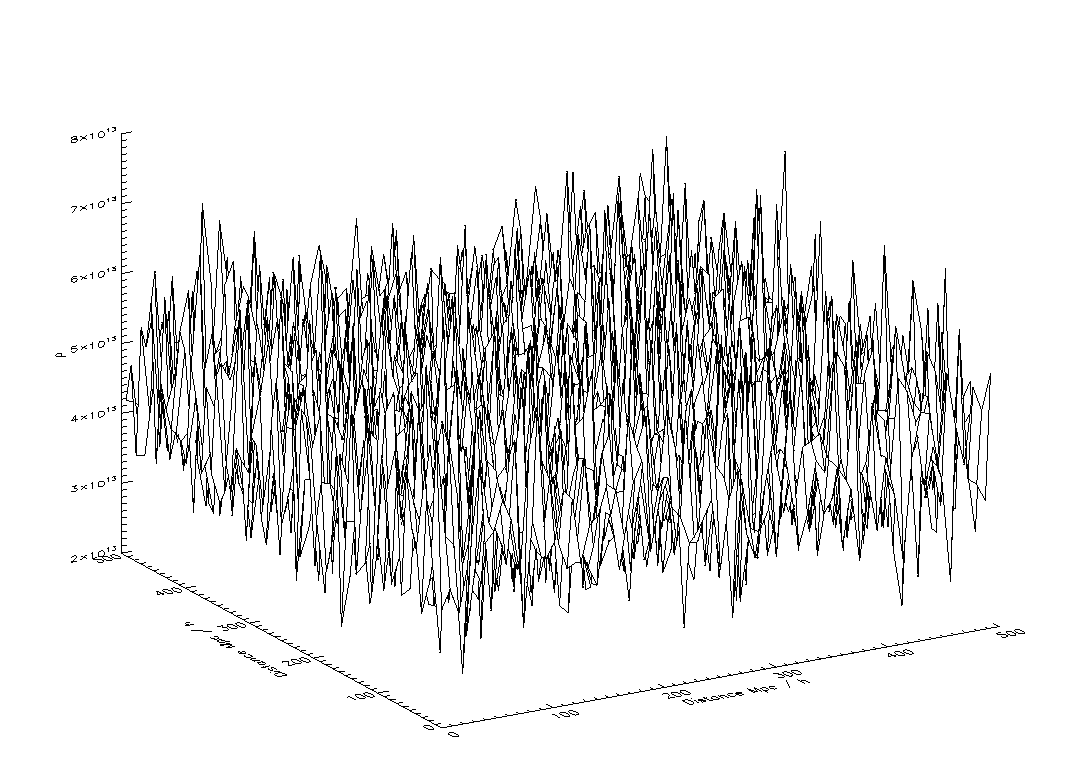
\includegraphics[width=0.49\columnwidth]{./full/wm64/rho/r00200}
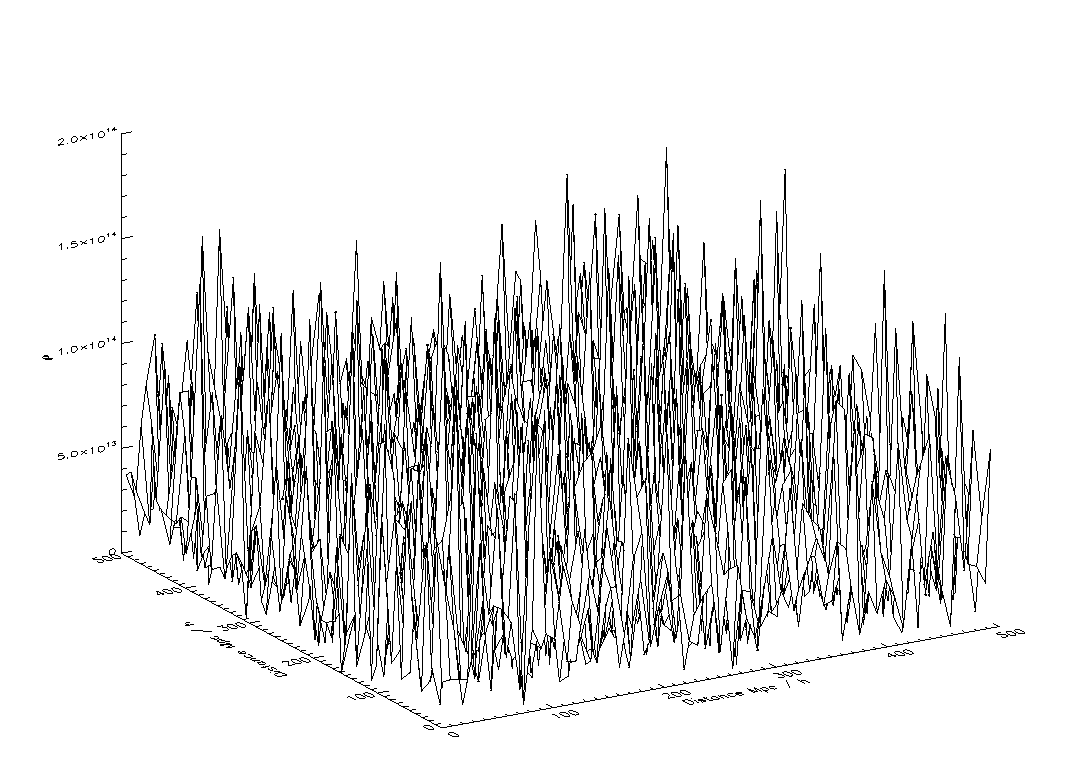
\includegraphics[width=0.49\columnwidth]{./full/wm64/rho/r01000}
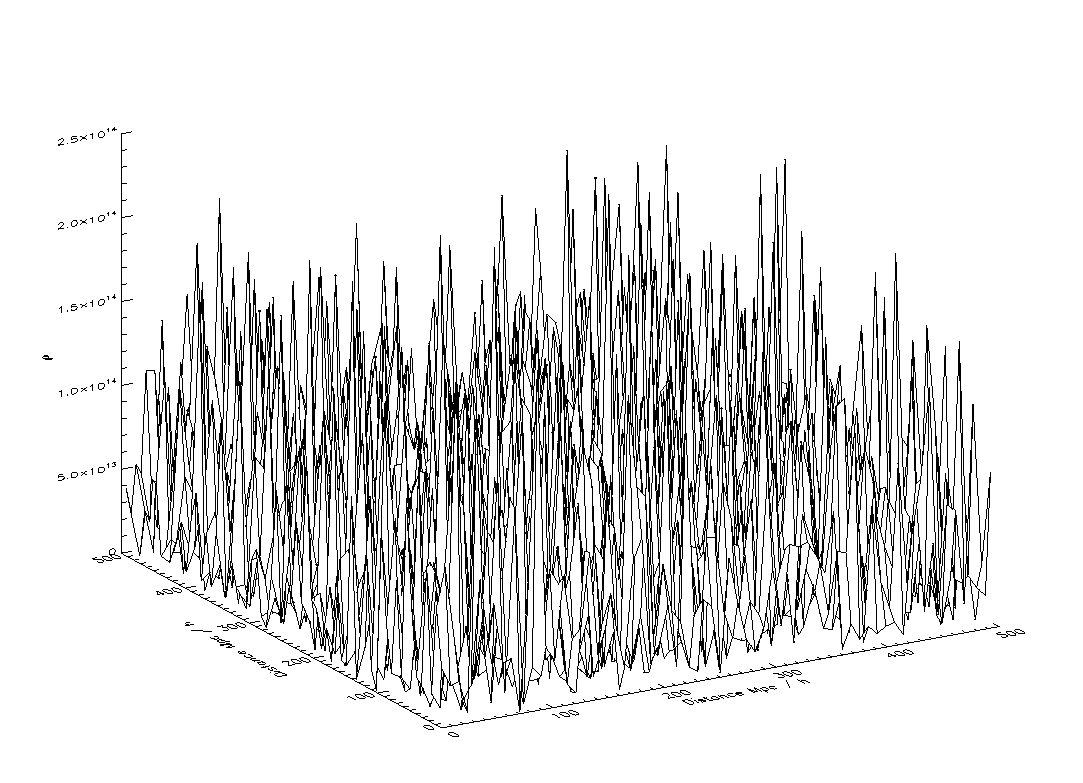
\includegraphics[width=0.49\columnwidth]{./full/wm64/rho/r02000}
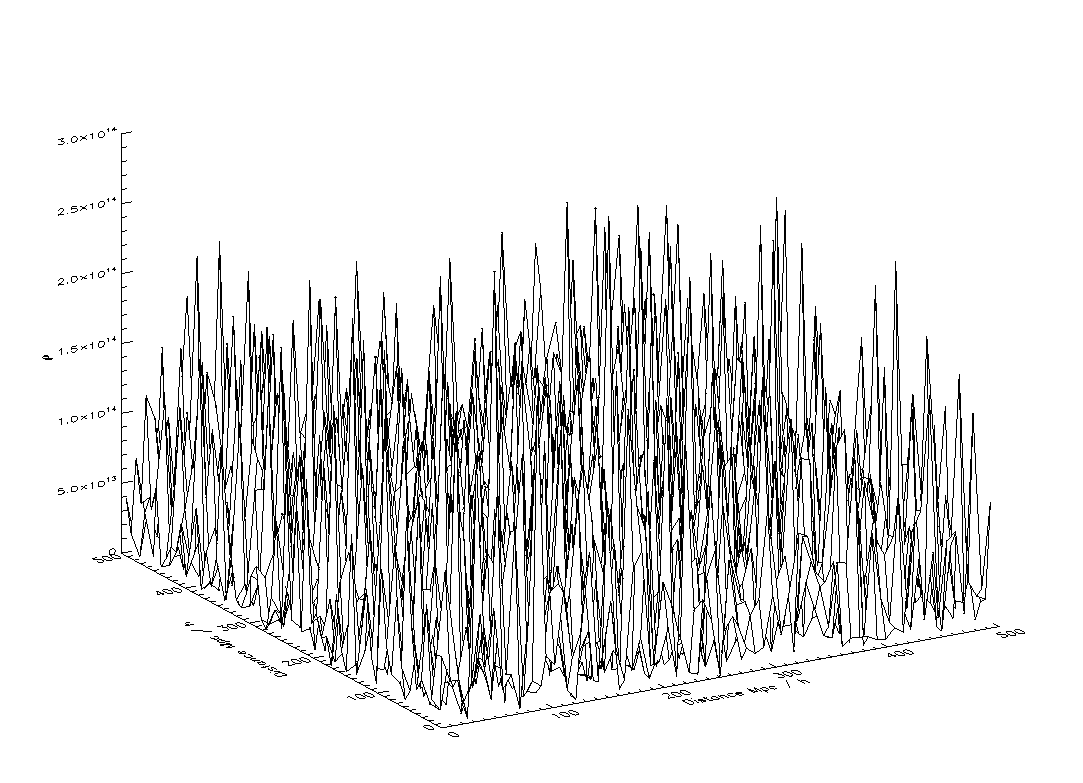
\includegraphics[width=0.49\columnwidth]{./full/wm64/rho/r03000}
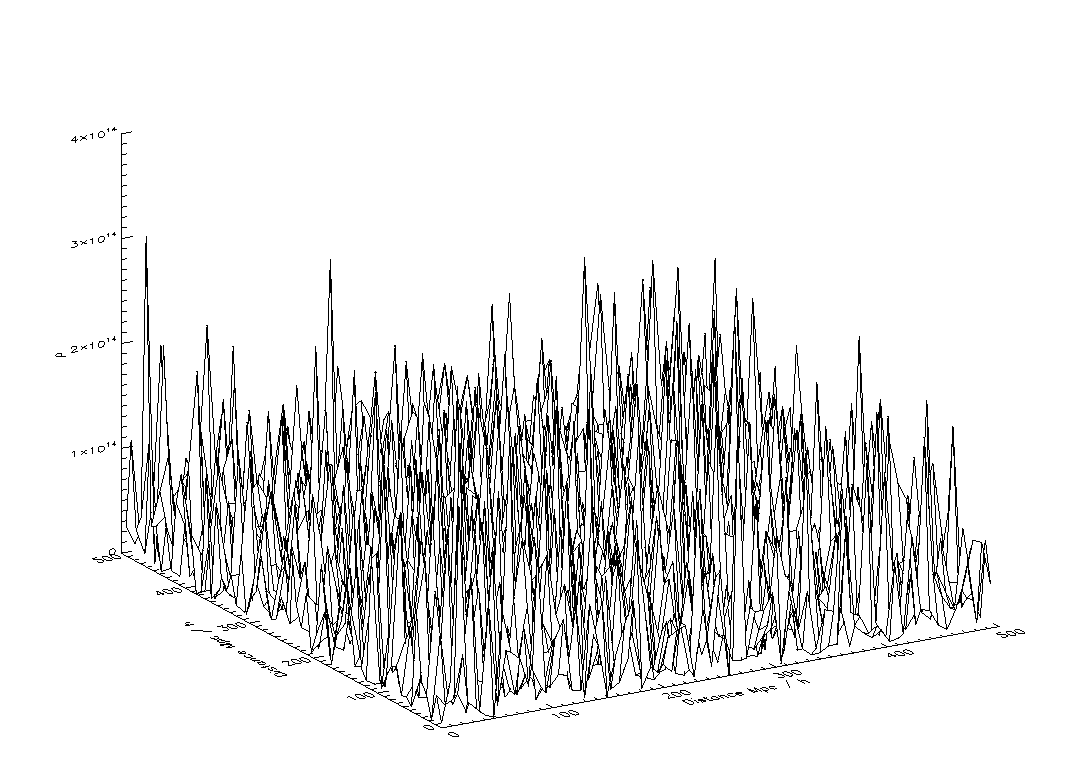
\includegraphics[width=0.49\columnwidth]{./full/wm64/rho/r03500}

   \end{center}
\caption{These plots show a surface plot of density $\rho$ from the wave-mechanics code. The outputs are for timesteps $0, 200, 1000, 2000, 3000, 3500$.}
\label{fig.wmrho}
\end{figure}

\begin{figure}[htb]
   \begin{center}
     %\leavevmode

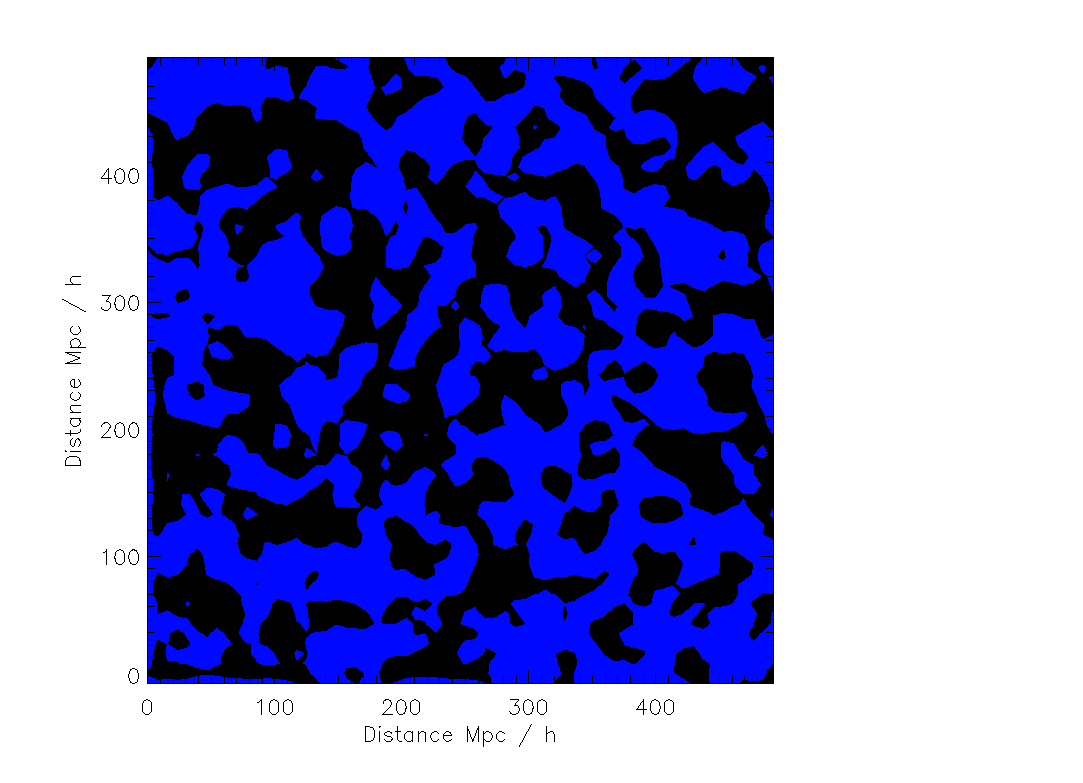
\includegraphics[width=0.49\columnwidth]{./full/wm64/rho_con/r00000_del_contour}
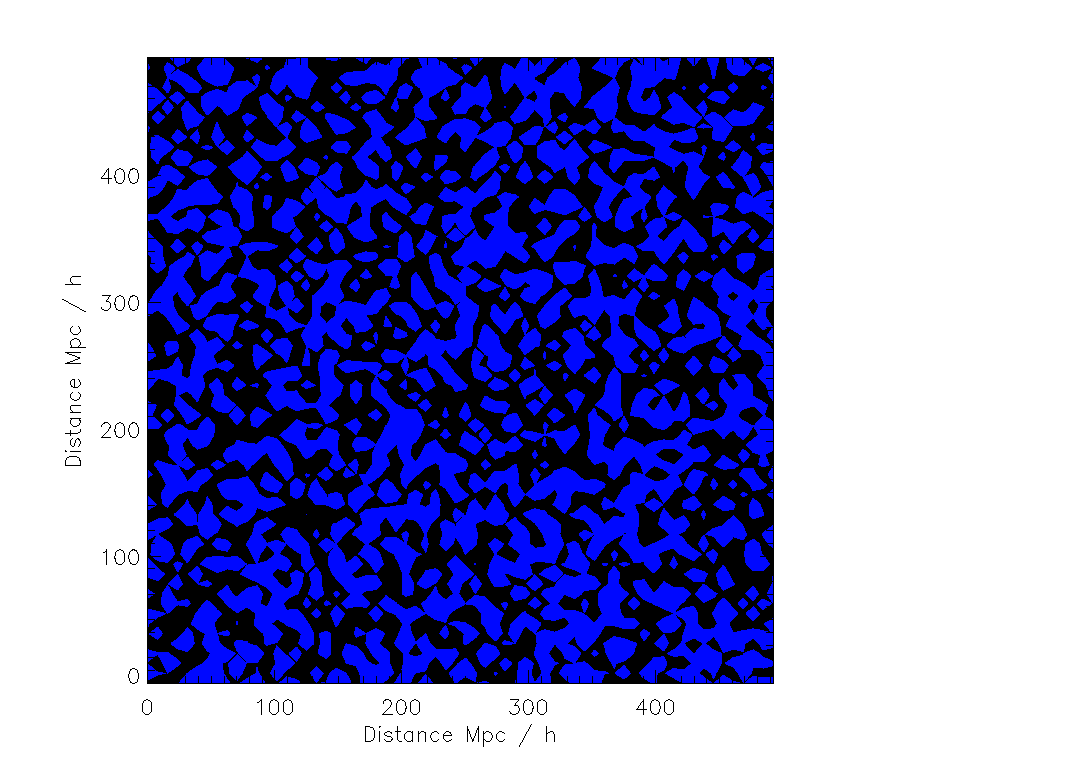
\includegraphics[width=0.49\columnwidth]{./full/wm64/rho_con/r00200_del_contour}
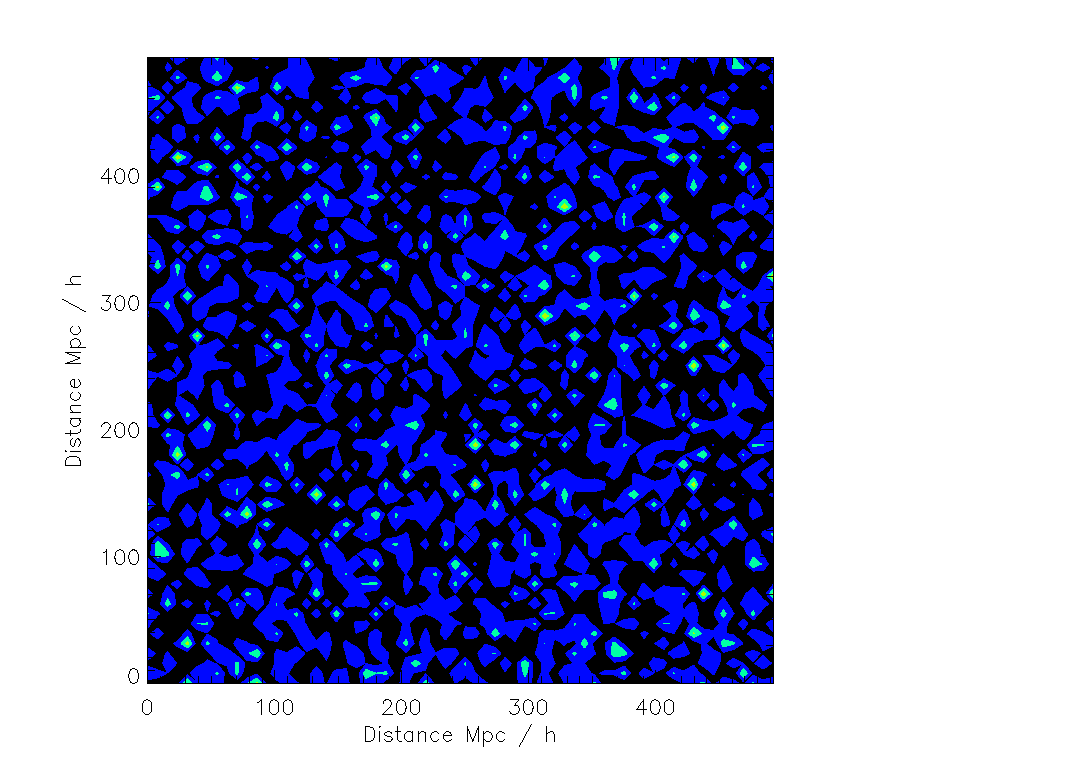
\includegraphics[width=0.49\columnwidth]{./full/wm64/rho_con/r01000_del_contour}
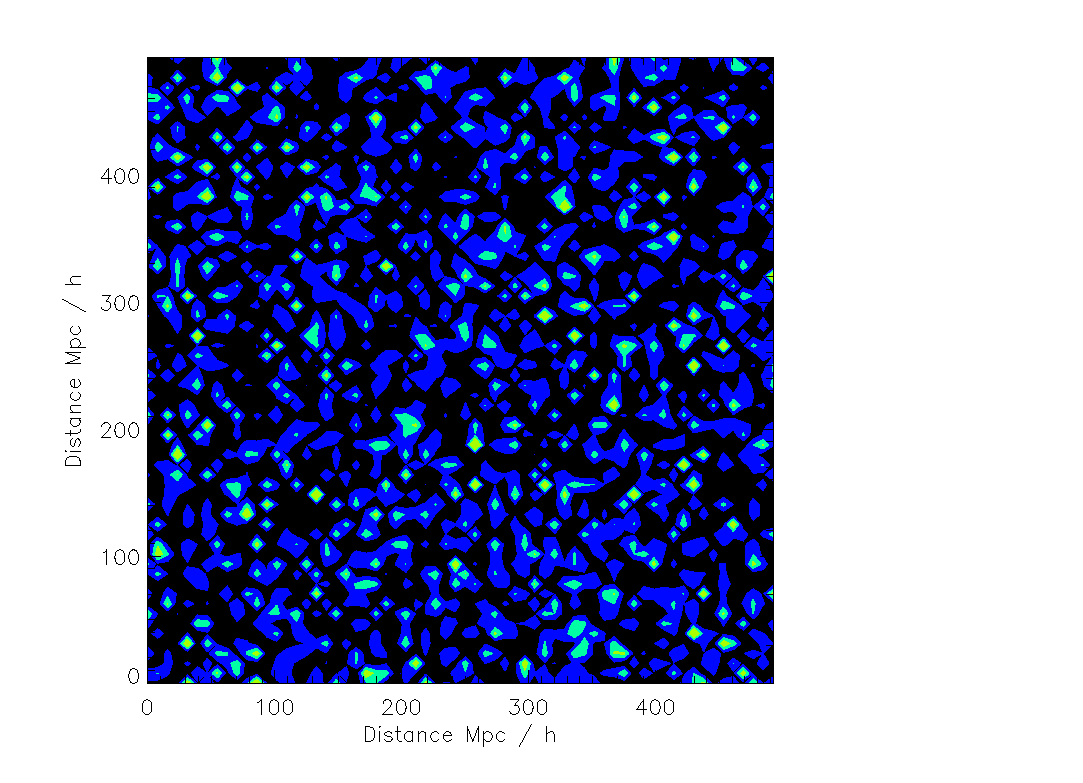
\includegraphics[width=0.49\columnwidth]{./full/wm64/rho_con/r02000_del_contour}
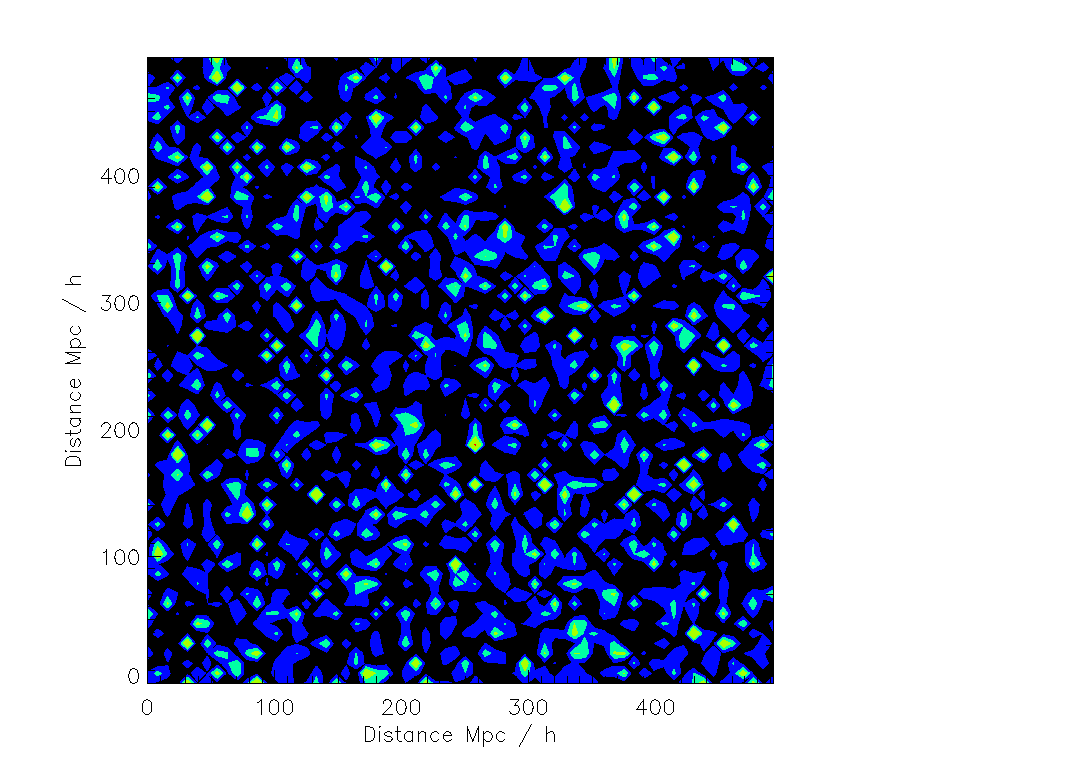
\includegraphics[width=0.49\columnwidth]{./full/wm64/rho_con/r03000_del_contour}
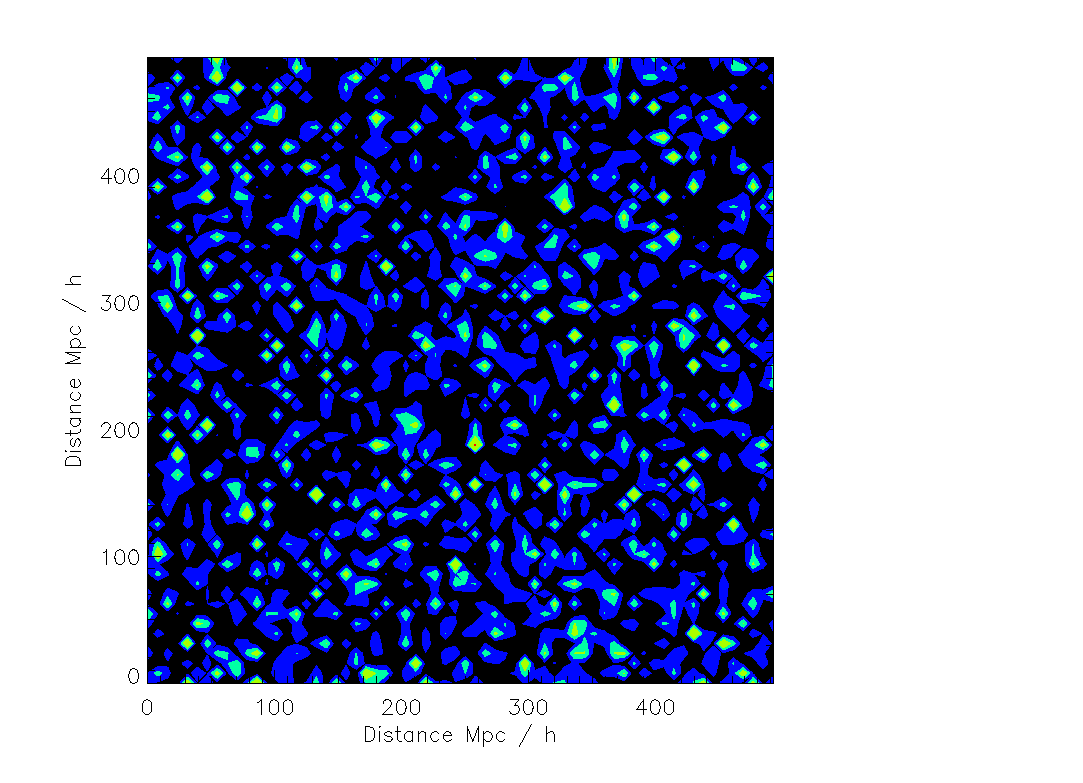
\includegraphics[width=0.49\columnwidth]{./full/wm64/rho_con/r03500_del_contour}

   \end{center}
\caption{These plots show a contour plot of density contrast ($\delta$) from the wave-mechanics simulation. The box length is $L = 500 \; {\rm Mpc / h}$ on each side. The contour levels are $\delta = -1, 0, 1, 2, 5$. The outputs are for timesteps $0, 200, 1000, 2000, 3000, 3500$.}
\label{fig.delta_contour}
\end{figure}

\begin{figure}[htb]
   \begin{center}
     %\leavevmode

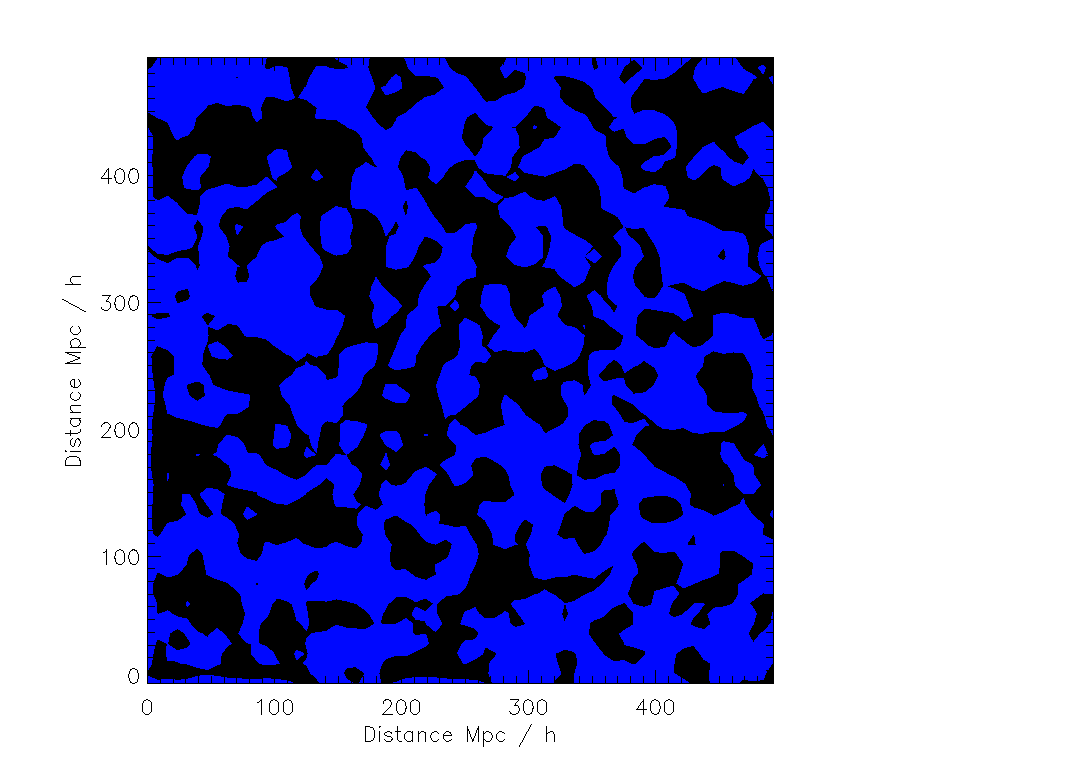
\includegraphics[width=0.49\columnwidth]{./full/gadget/contour/del_contour0000}
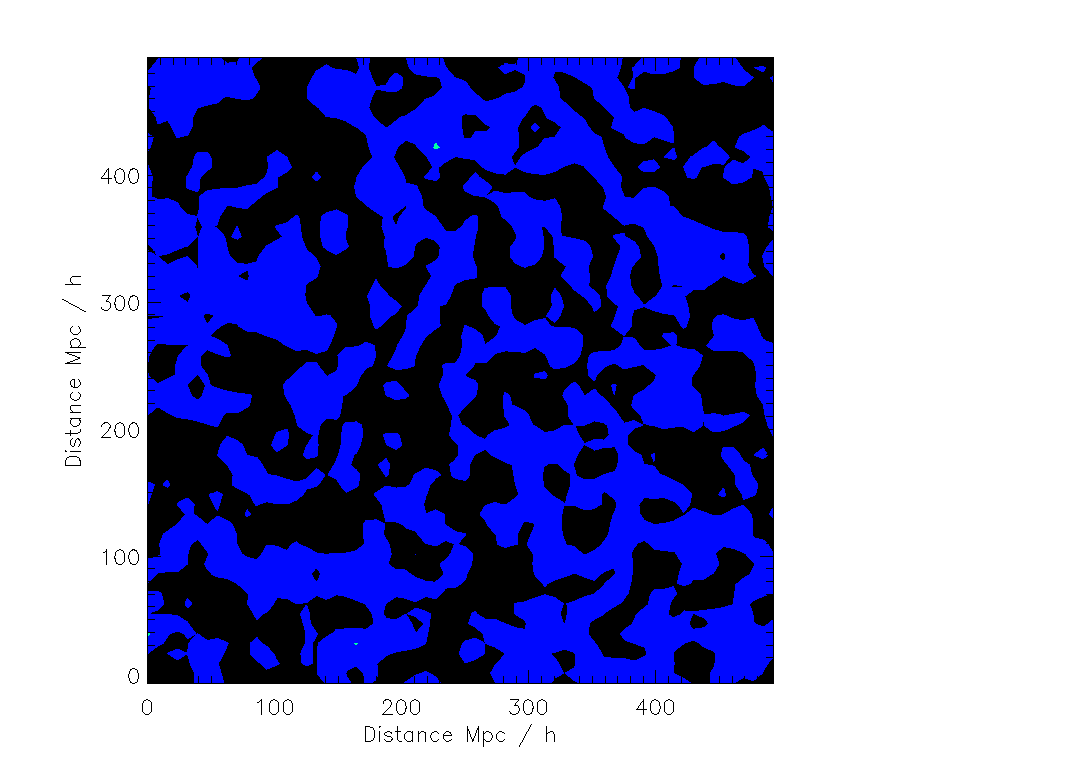
\includegraphics[width=0.49\columnwidth]{./full/gadget/contour/del_contour000}
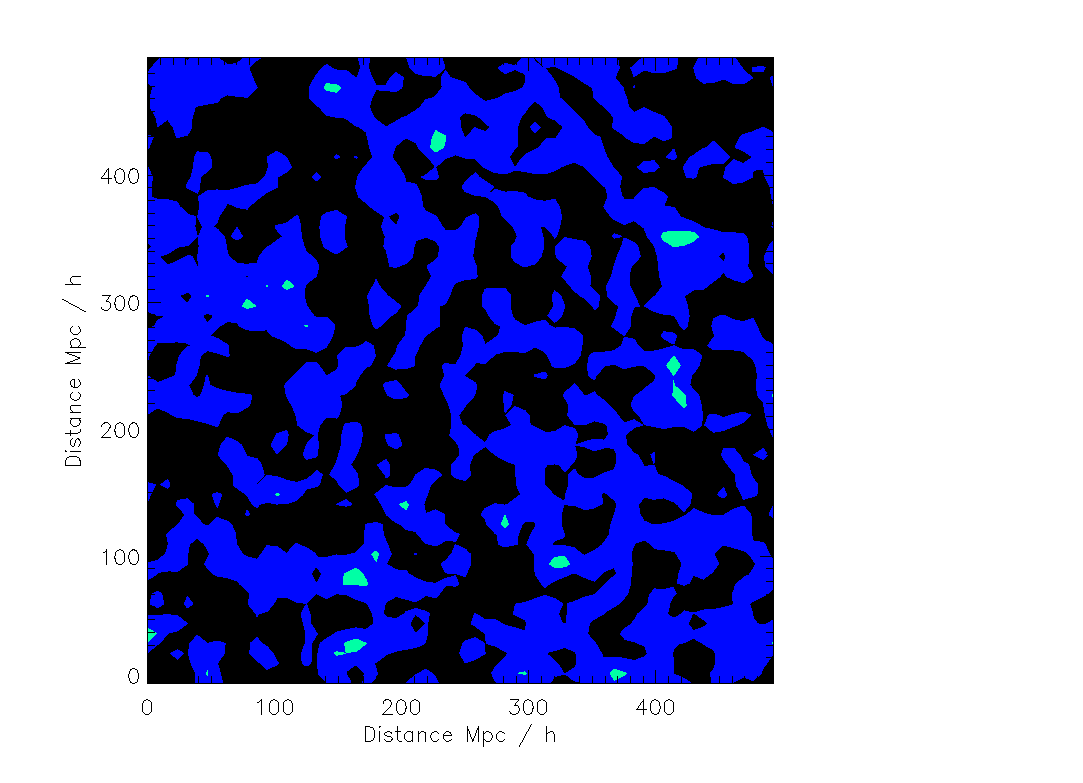
\includegraphics[width=0.49\columnwidth]{./full/gadget/contour/del_contour001}
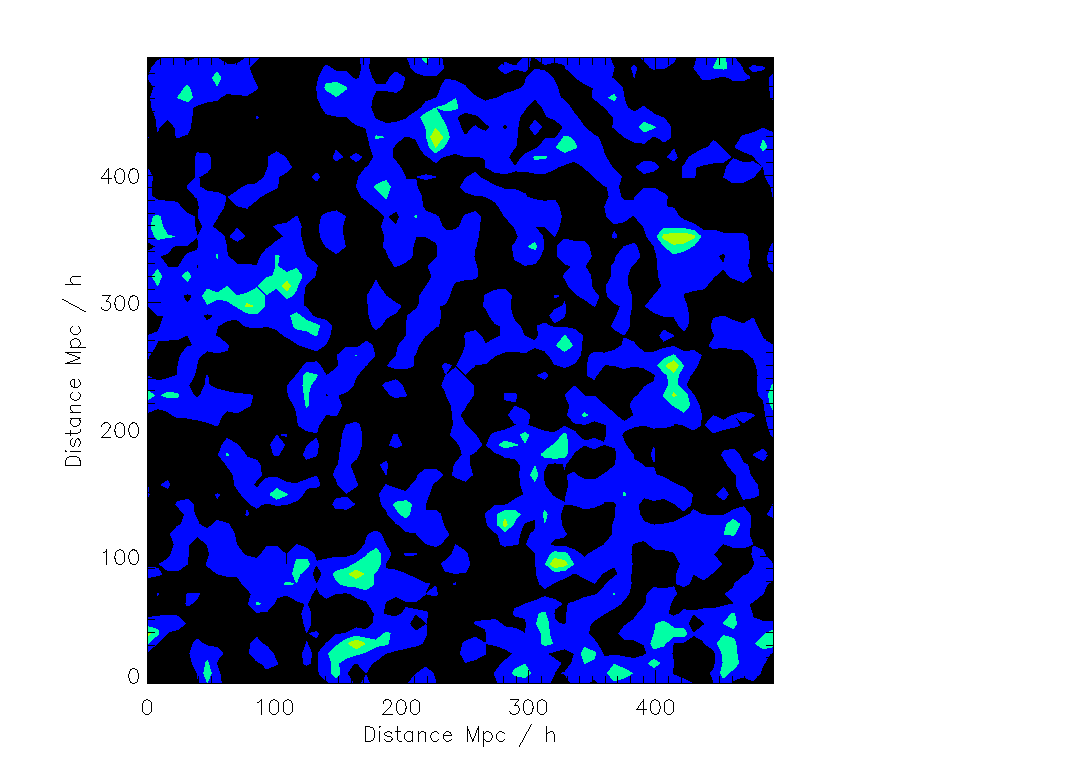
\includegraphics[width=0.49\columnwidth]{./full/gadget/contour/del_contour002}
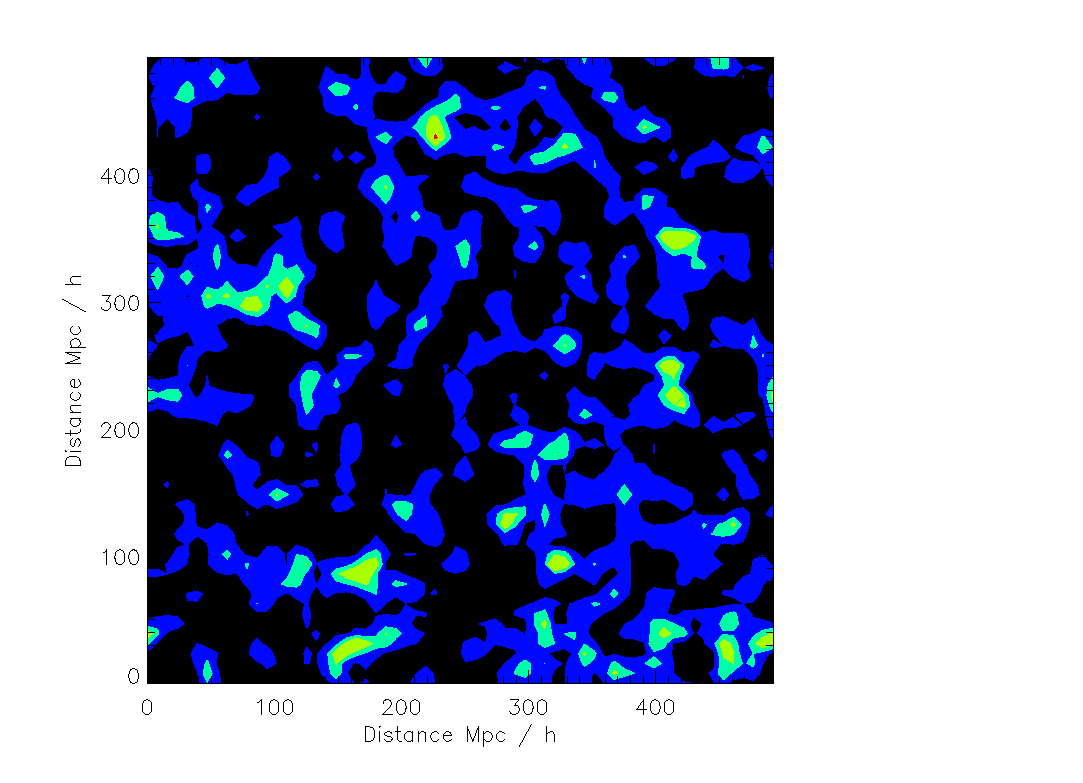
\includegraphics[width=0.49\columnwidth]{./full/gadget/contour/del_contour003}
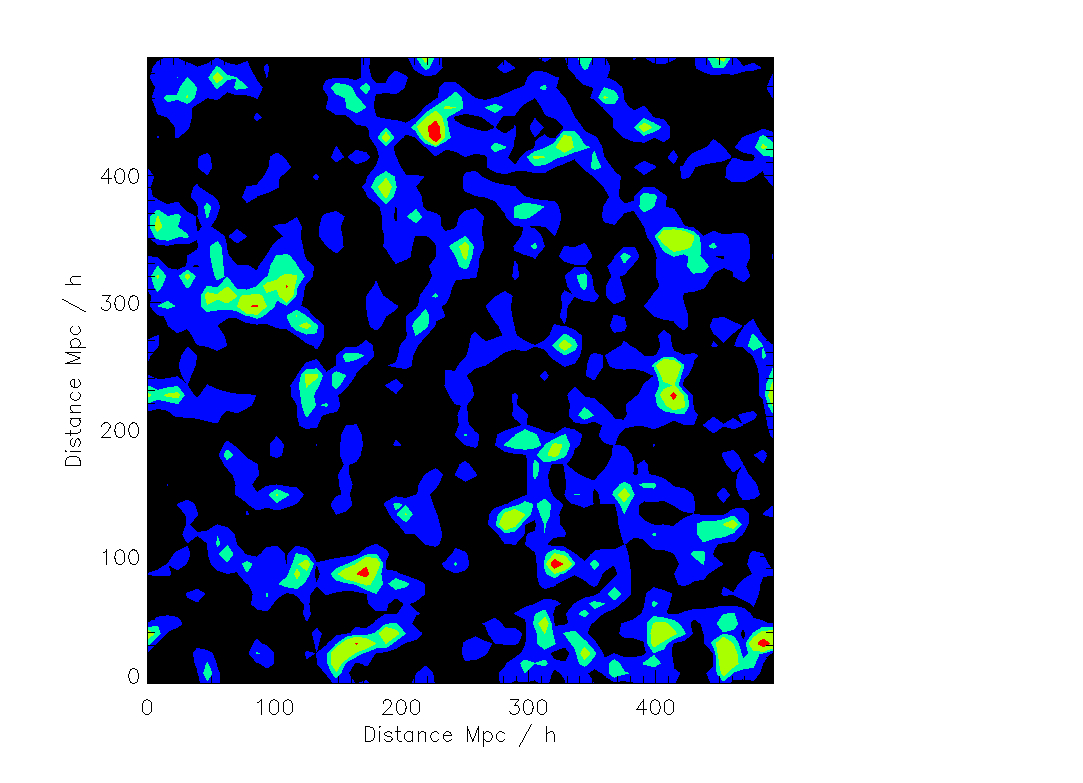
\includegraphics[width=0.49\columnwidth]{./full/gadget/contour/del_contour004}

   \end{center}
\caption{These plots come from the GADGET-2 simulation and show a contour plot of density contrast ($\delta$). The box is $500 \; {\rm Mpc / h}$ on each side. The contour levels are $\delta = -1, 0, 1, 2, 5$.}
\label{fig.gadget_contour}
\end{figure}


\subsubsection{Gaussian smoothing}
\noindent The Gaussian smoothing described in this section is applied as a post-processing diagnostic tool for comparing outputs between codes; it is not part of the physical evolution of the wave-mechanics simulation itself.

Given the magnitude of the over-densities in the initial condition $|\delta|_{\rm initial} \sim 0.3$ we previously suppressed this value by dividing the values across the whole field by 10. This was an arbitrary choice, however in cosmology there is an accepted standard for smoothing that advocates smoothing the data with a gaussian window with a standard deviation of  $\sigma = 8$ Mpc. It is an accepted standard because, statistically, all structures larger than 8 Mpc are roughly linear.

This method of smoothing was chosen and applied to both the initial density field and to the output density fields. The smoothed initial density field was supplied to the wave-mechanics code for another run of the simulation to be performed.

The smoothing operation is defined in the following way:
\begin{equation}
\rho_{gauss} = \frac{1}{W} \sum_{-\sigma_z}^{\sigma_z} \sum_{-\sigma_y}^{\sigma_y} \sum_{-\sigma_x}^{\sigma_x} \rho_{TSC}\; e^{\left(\frac{-(r-r')^2}{2 \sigma^2} \right)}
\end{equation}

\noindent here $\rho_{gauss}$ is new smooth field and $\rho_{TSC}$ is the density field as generated by the TSC smoothing routine in case of the GADGET-2 outputs. Recall that the TSC routine smooths particle positions onto a uniform grid and hence gives a continuous density field. The weight, $W$, is defined as:
\begin{equation}
W = \sum_{-\sigma_z}^{\sigma_z} \sum_{-\sigma_y}^{\sigma_y} \sum_{-\sigma_x}^{\sigma_x} e^{\left(\frac{-(r-r')^2}{2 \sigma^2} \right)}
\end{equation}

\noindent where it is already assumed that we will truncate the gaussian to a certain precision, in this case 3 standard deviations ($\sigma$). In the simulation performed, a physical length of $500$ Mpc was chosen, and the resolution was $64^3$. This means that one pixel has a length of $7.8$ Mpc hence 3 pixels roughly corresponds to 3 standard deviations.

Figures \ref{fig.gadgauss} \& \ref{fig.wmgauss} show contour plots of over-density, $\delta$, from GADGET-2 and wave-mechanics respectively. The peaks have been well smoothed out by roughly a factor of 6. The contour levels are black for $\delta < 0$ and blue for $\delta \geq 0$. The results for GADGET-2 look almost static over the full run of the simulation but there is some movement within the structure.

The results for wave-mechanics look less random at later times, there are definite structures in the smoothed density fields at late times ($a \sim 1$). In the previous unsmoothed outputs (such as figure \ref{fig.wmhistdc}) long-term structure was not as distinguishable as in these newer results.

The problem seems to have been due to the initial density peaks being too high for our chosen resolution. The maximum over-density peak was $\delta \sim 0.3$ in the original initial conditions, here in the smoothed initial condition it is $\sim 0.05$. The growth of the maximum value of $\delta$ is also much slower and reaches a maximum of $\delta = 9.1$ in the final output. This is comparable to the unsmoothed initial density field of wave-mechanics in the previous section. The big improvement now is that the outputs from wave-mechanics look closer to those from GADGET-2 (after gaussian smoothing).

Like previous results we can see regions of multi-streaming which resemble an interference pattern. The outputs from wave-mechanics are noticeably less clean but this isn't a surprise given the added complexity inherent in wave-mechanics and the fact that we are now dealing with a continuous density field.


\begin{figure}[htb]
   \begin{center}
     %\leavevmode
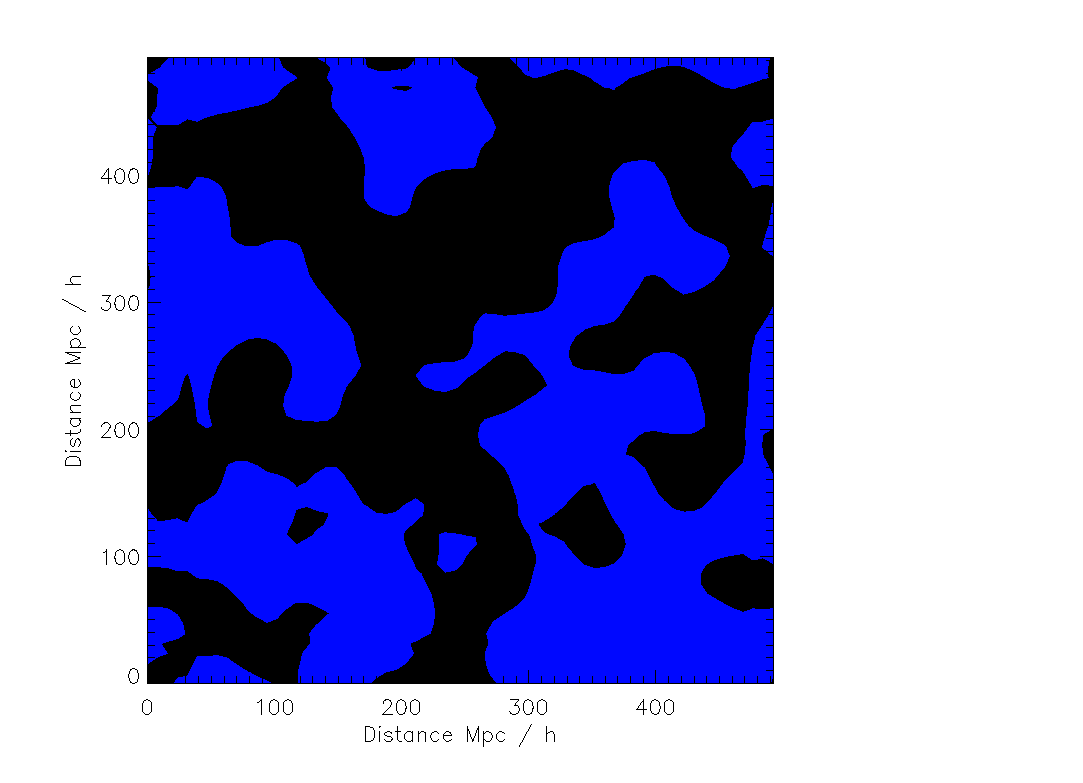
\includegraphics[width=0.45\columnwidth]{./full/gadget/gaussian/0000_del_contour}
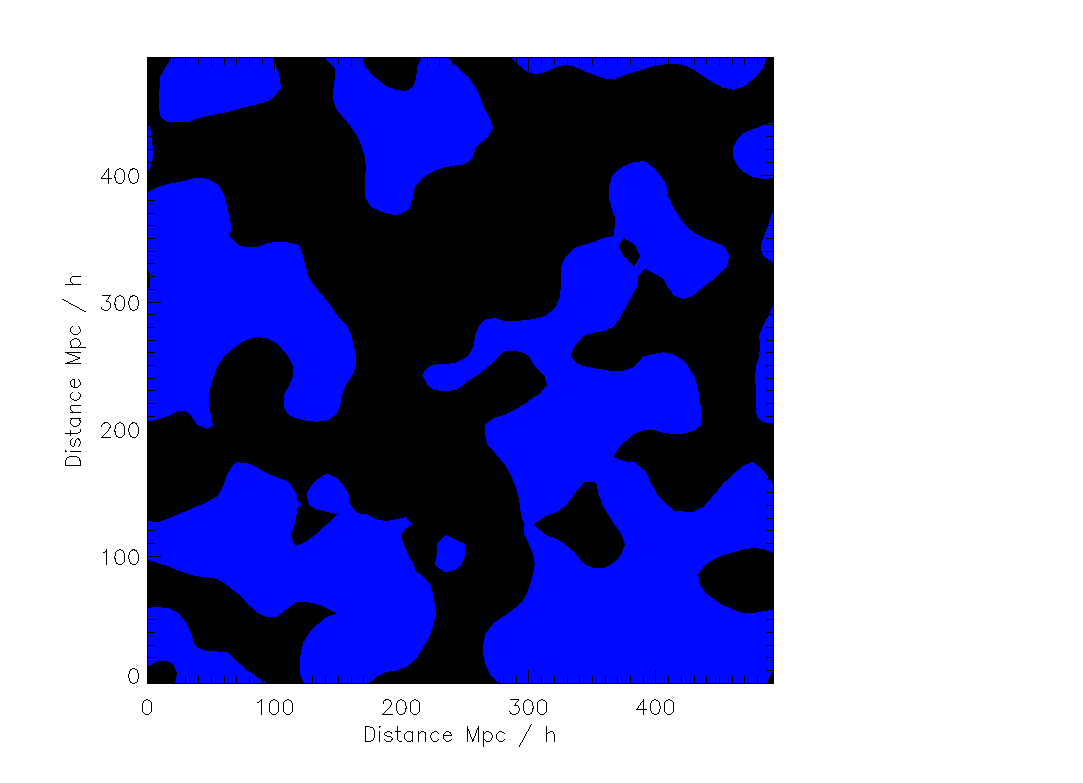
\includegraphics[width=0.45\columnwidth]{./full/gadget/gaussian/000_del_contour.eps}
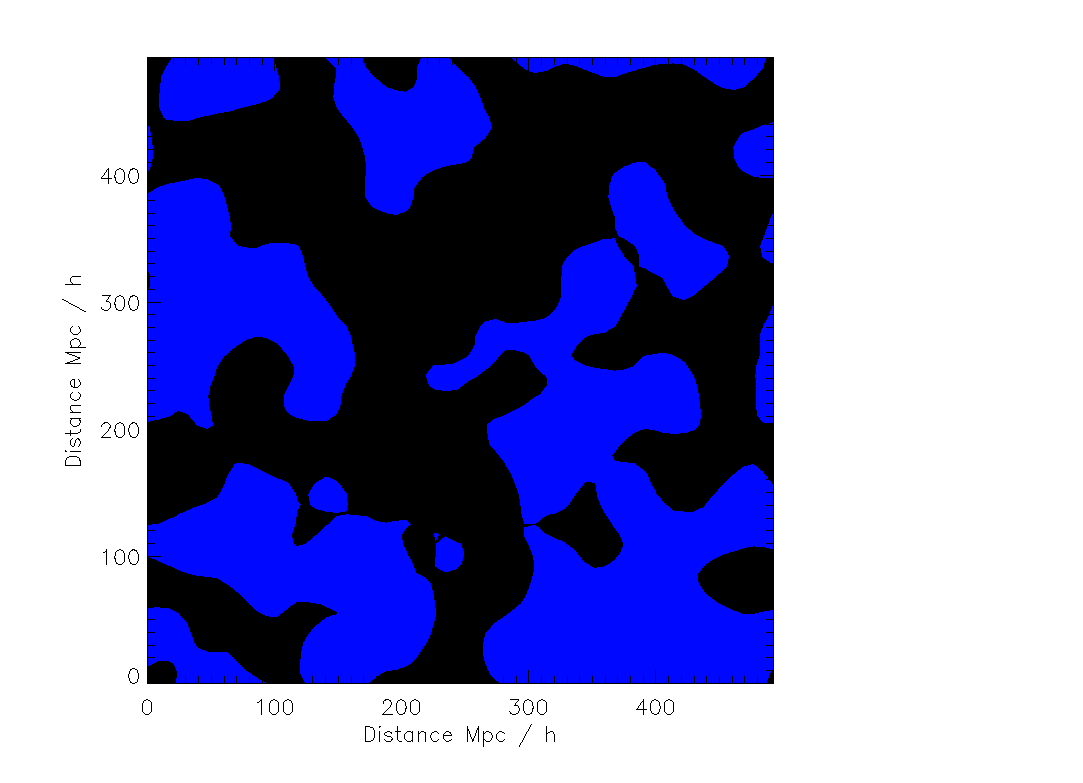
\includegraphics[width=0.45\columnwidth]{./full/gadget/gaussian/001_del_contour.eps}
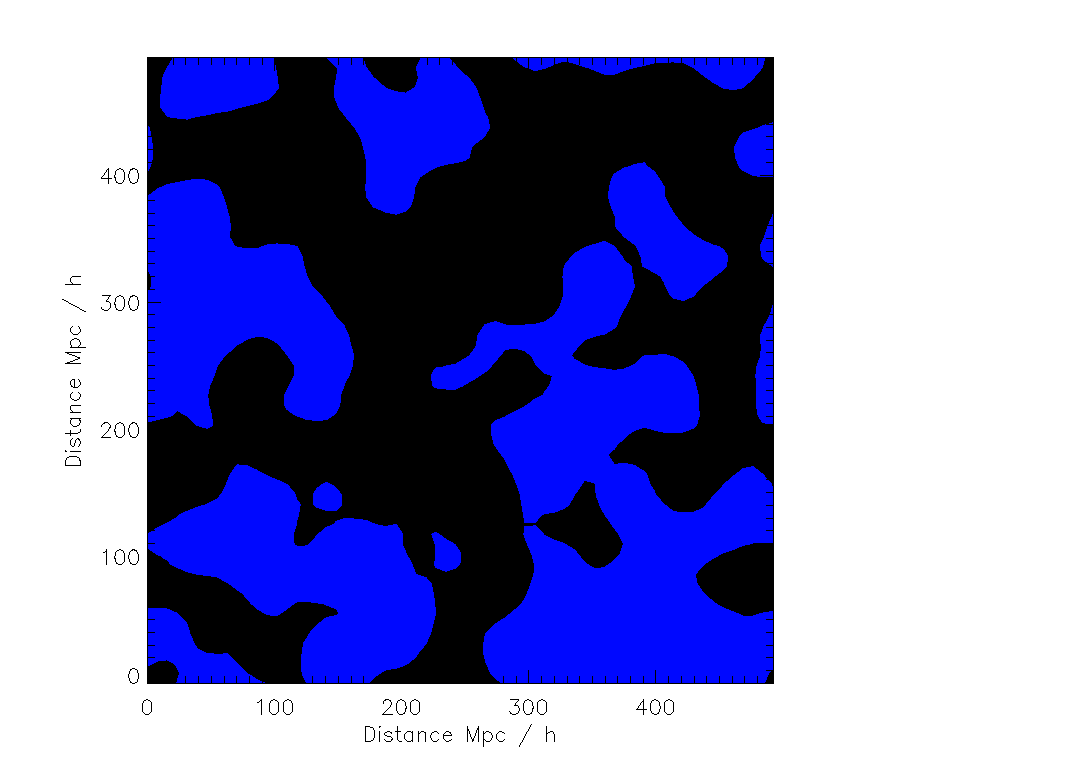
\includegraphics[width=0.45\columnwidth]{./full/gadget/gaussian/002_del_contour.eps}
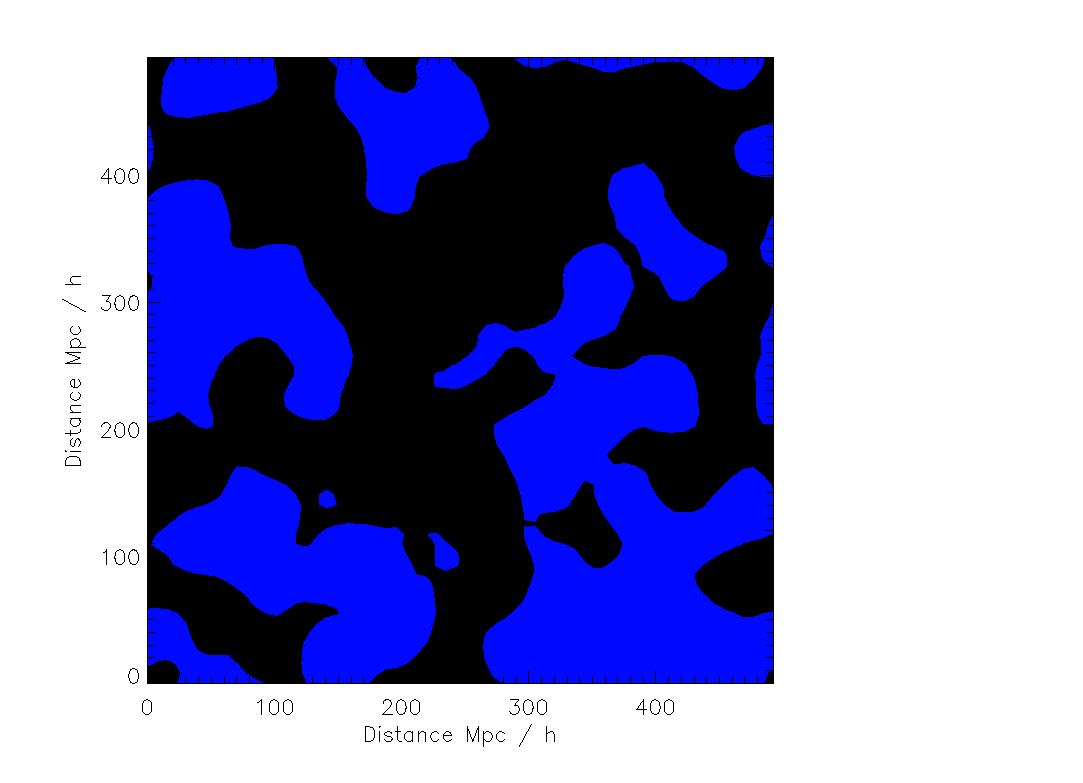
\includegraphics[width=0.45\columnwidth]{./full/gadget/gaussian/003_del_contour.eps}
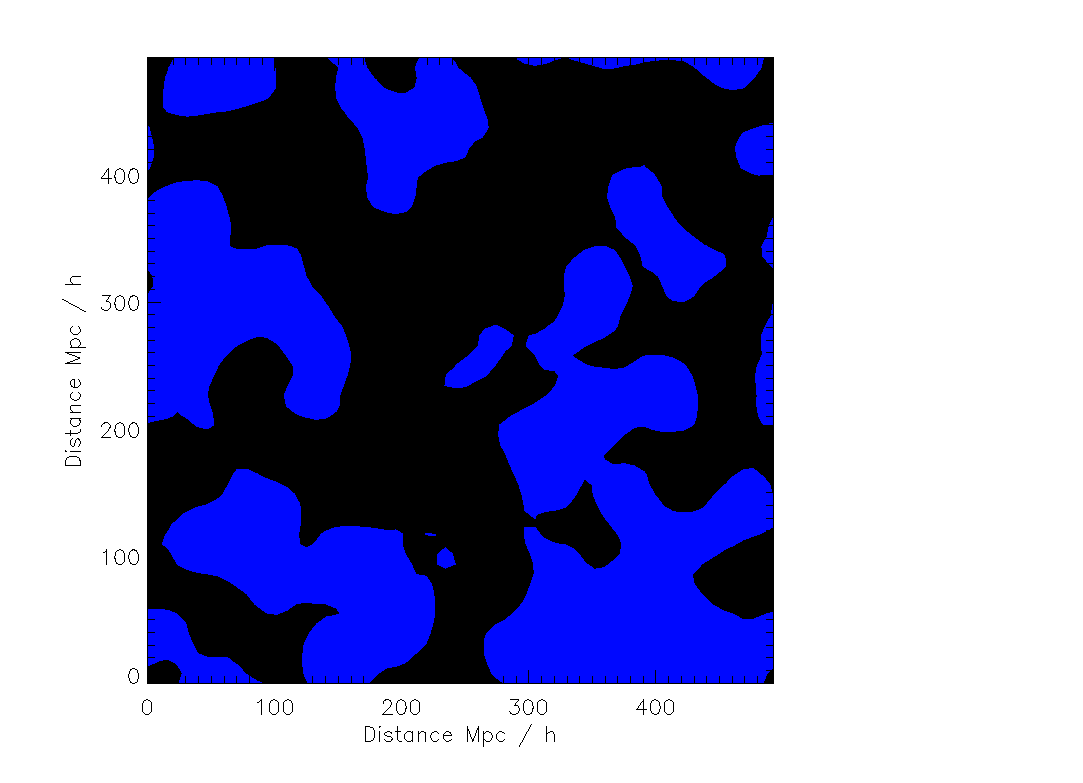
\includegraphics[width=0.45\columnwidth]{./full/gadget/gaussian/004_del_contour.eps}

   \end{center}
\caption{This series of contour plots shows the previously seen GADGET-2 outputs for over-density ($\delta$) after gaussian smoothing has been applied. $z = 32, 3, 2, 1, 0.5, 0.05$. The contour levels are black for $\delta < 0$ and blue for $\delta \geq 0$.}
\label{fig.gadgauss}
\end{figure}


\begin{figure}[htb]
   \begin{center}
     %\leavevmode
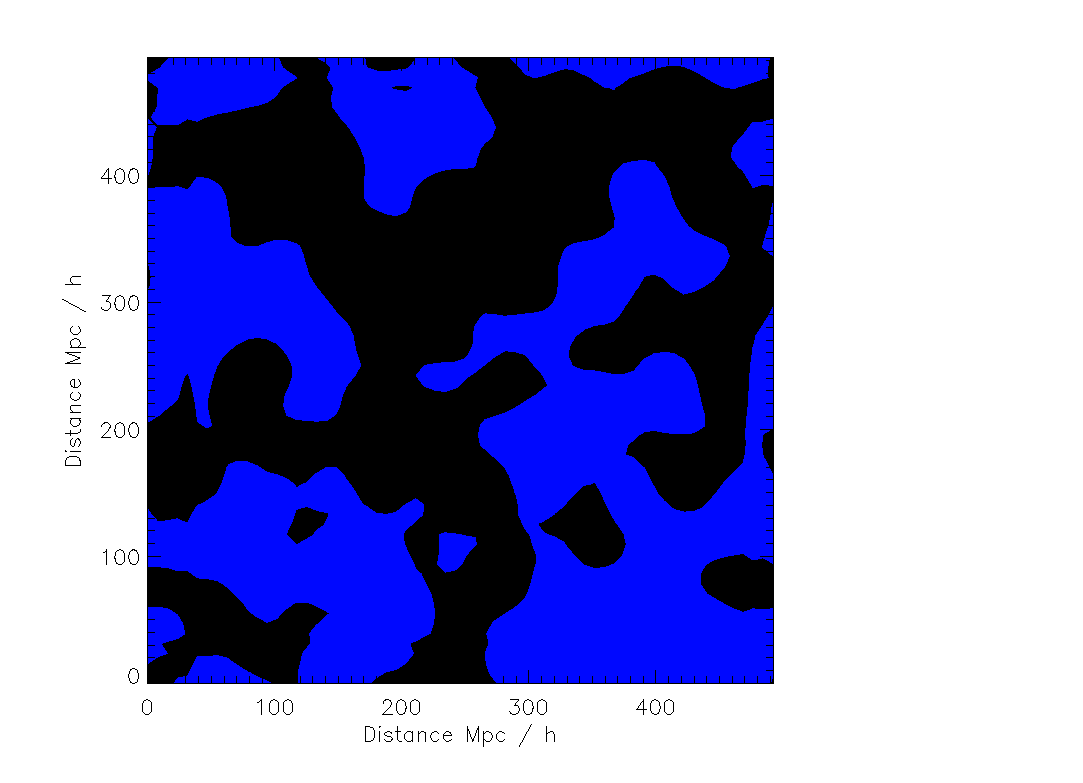
\includegraphics[width=0.45\columnwidth]{./full/wm64/rho_gauss/00000_del_contour}
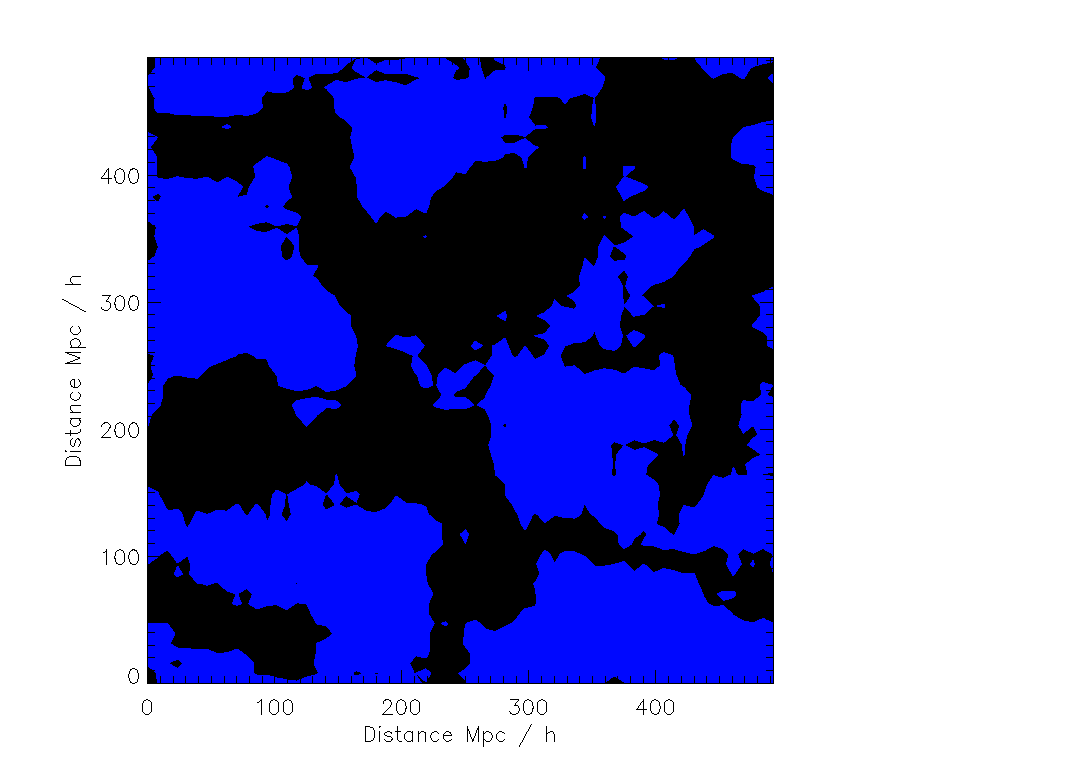
\includegraphics[width=0.45\columnwidth]{./full/wm64/rho_gauss/00200_del_contour}
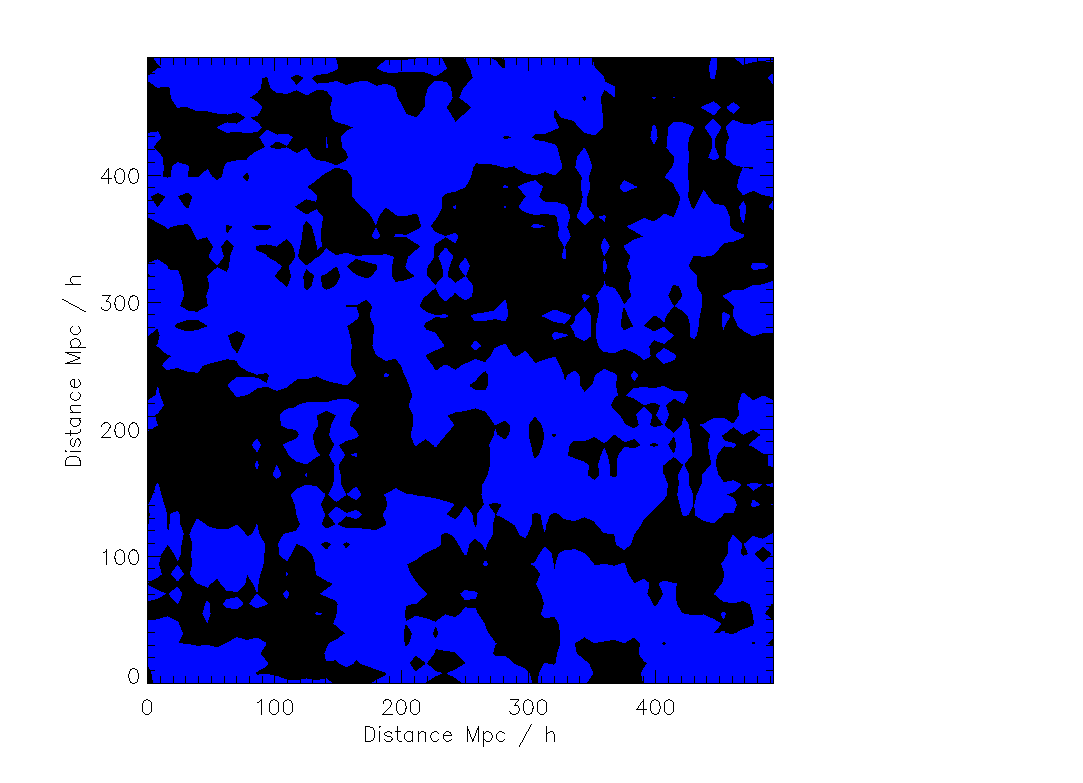
\includegraphics[width=0.45\columnwidth]{./full/wm64/rho_gauss/01000_del_contour}
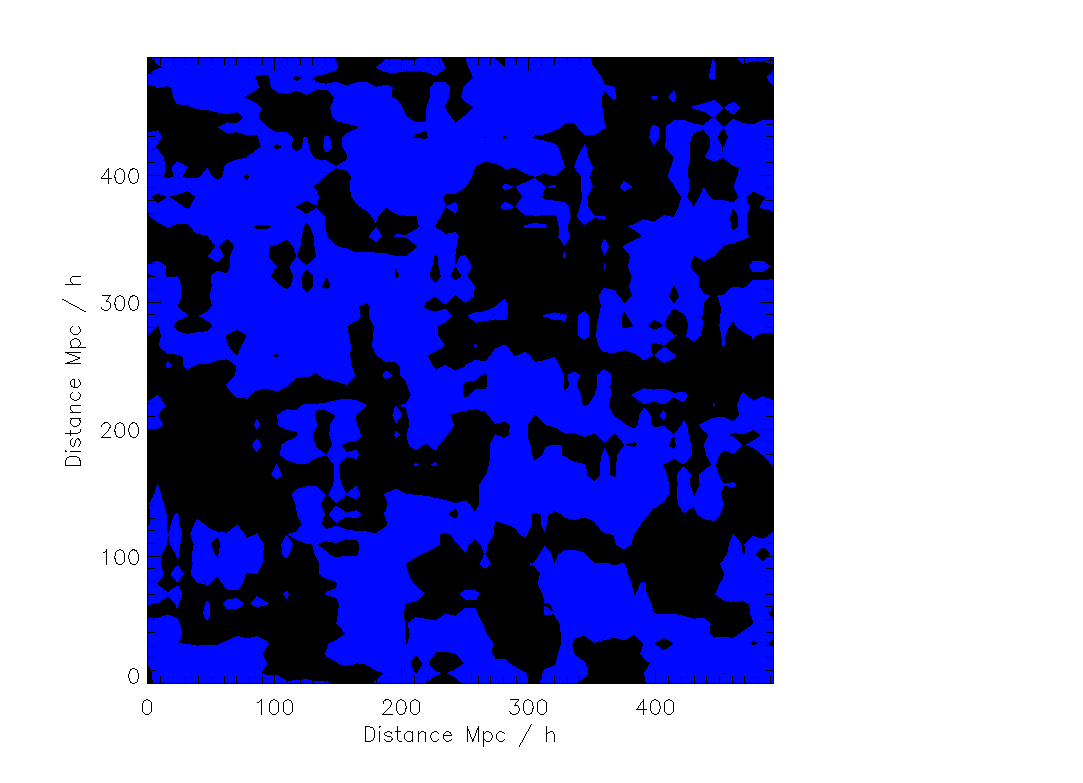
\includegraphics[width=0.45\columnwidth]{./full/wm64/rho_gauss/02000_del_contour}
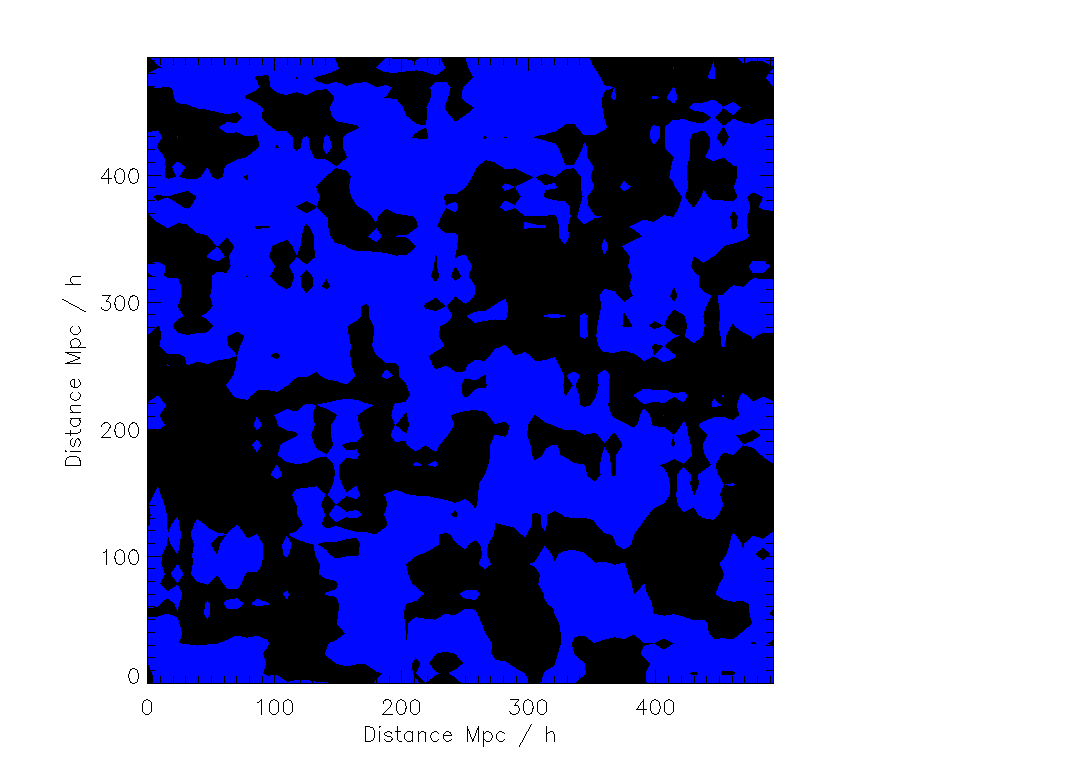
\includegraphics[width=0.45\columnwidth]{./full/wm64/rho_gauss/03000_del_contour}
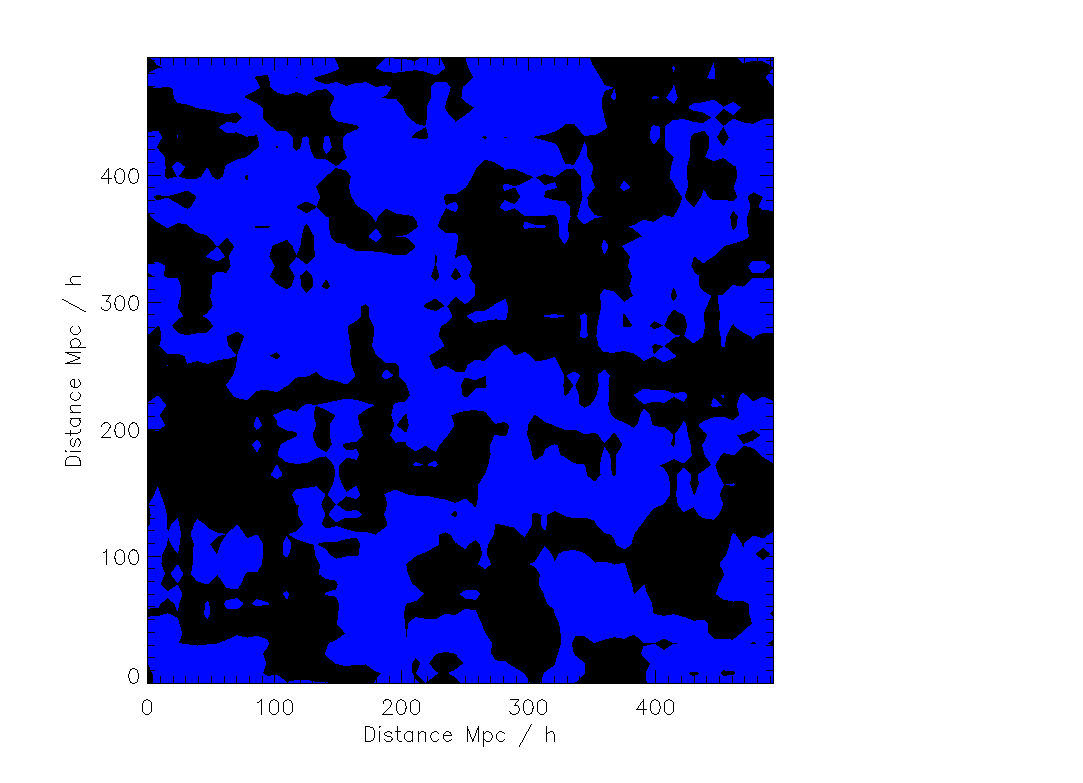
\includegraphics[width=0.45\columnwidth]{./full/wm64/rho_gauss/03500_del_contour}

   \end{center}
\caption{This series of contour plots shows the previously seen wave-mechanics outputs for over-density ($\delta$) after gaussian smoothing has been applied. The outputs at $t = 0, 200, 1000,$ $2000, 3000, 3500$ ($a = 0.03125,0.038,$ $0.085,0.23, 0.63, 1.03$). The contour levels are black for $\delta < 0$ and blue for $\delta \geq 0$. }
\label{fig.wmgauss}
\end{figure}


\subsubsection{Robustness of results --- conserved quantities}
\label{ch_5_robust}
Given the high variability of density peaks spatially, it is not apparent that the code is well-behaved. Hence it is worth performing consistency checks, such as plotting histograms but as mentioned through out this thesis we are ideally concerned with conserved physical quantities. The stability and robustness of the wave-mechanics code is verified by the conservation of mass and momentum. Over the whole simulation from the initial conditions until redshift $z = 0$ (3500 timesteps), the variation of mass is less than 7 significant figures. While momentum conservation (denoted by $P$) is only slightly worse but an unnoticeable effect in the simulation. Mass and momentum conservation are necessary but not sufficient conditions for a reliable simulation; energy conservation is an independent requirement that follows from the symplectic nature of the integration scheme (as discussed in Chapter \ref{ch_2}). Figure \ref{fig.conserve} shows how these quantities vary over the course of the simulation.

The quantities were calculated as follows:

\begin{eqnarray}
M_{\rm total} &=& \int^V \psi \psi^* \; dx^3 \\
P_{\rm total} &=& -i\nu \int^V \psi^* \nabla \psi \; dx^3
\end{eqnarray}

Naturally, these quantities have regimes where they are not conserved and the code is has huge errors. The regimes of stability are dictated by the resolutions lengths $dx$ and $dt$ as with any finite difference (or finite element) code. However, there is an additional parameter that dictates stability: $\nu$. When $\nu$ is relatively large (as dictated by choice of $n_g$, the number of gridpoints per side) then the dispersion of the wavefunction is higher but if this value is too large then the wavefunction allows for matter to move too quickly. When this happens, mass and momentum are no longer conserved.


\begin{figure}[htb]%[tp]%[htb]
   \begin{center}
    % \leavevmode
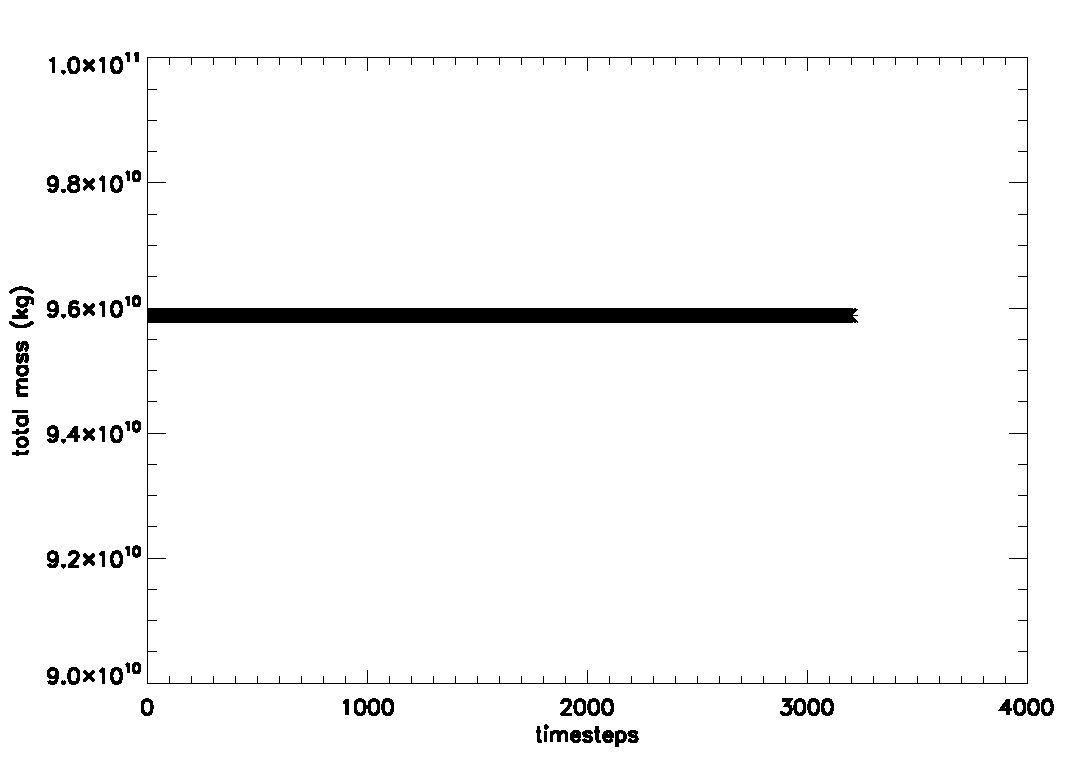
\includegraphics[width=0.49\columnwidth]{./full/wm64/tot_mass3200}
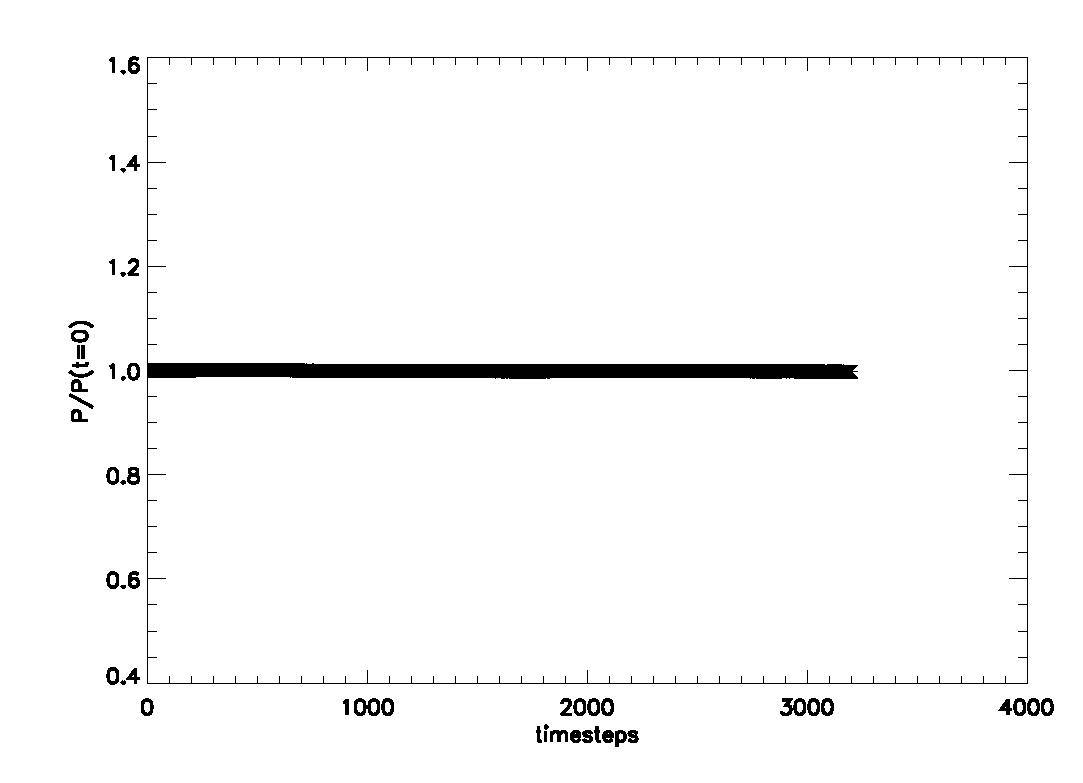
\includegraphics[width=0.49\columnwidth]{./full/wm64/normed_tot_mom3200}
   \end{center}
\caption{The conservation of total mass (left) and total momentum (right) over time in the wave-mechanics code. The flatness of the distribution shows that the quantities do not vary significantly over time.}
\label{fig.conserve}
\end{figure}

\section{Velocity \& Vorticity}
The main focus of this section is to show the comparison between  the ``industry standard'' code, GADGET-2, and our own wave-mechanics code. In figure \ref{fig.gadvel} we present the velocity in the form of histograms of the $x$ component of velocity. From symmetry we require that the other velocity components, $y \; \& \; z$, have the same shape (height and width) at all output times. The histograms of the other velocity components confirm this is the case; for brevity, those plots have been omitted from this thesis.

Overplotted on each of the GADGET-2 velocity histograms is that of a theoretical gaussian with the same amplitude and standard deviation. We can see very good agreement between the data and the theoretical gaussian. The velocity data from the GADGET-2 output files requires a simple scaling in order to calculate the real physical velocities: $v_{real} = \sqrt{a} v_{code}$ (km/s).

The velocity from the wave-mechanics code can be calculated using the probability current as given by equation \ref{eqn_j}. This technique was presented as the big difference between my FPA code that that of Short \citep{bib_short}. We have shown that the velocity from the probability current is consistent with the results of Short who used a phase unwrapping technique. As shown in Chapter \ref{ch_3}, we can use a simpler form of the probability current:

\begin{equation}
\underline{v} = \frac{\hbar}{m} \Im\left(\frac{\nabla \psi}{\psi}\right)
\end{equation}

Figure \ref{fig.wmvel} shows a series of graphs of the $x,y$ components of velocity (at a fixed value of $z$) and correspond to the density and over-density plots from the wave-mechanics code shown above (figures \ref{fig.wmrho} \& \ref{fig.delta_contour}, respectively). The velocities at earlier times appear isotropic as expected and of roughly equal magnitude (with a gaussian distribution).

For comparison with the GADGET-2 histograms (\ref{fig.gadvel}), I also provide histograms for the $x$ component of velocity from the wave-mechanics code. It also appears as a gaussian at earlier times by evolves in a slightly different way to GADGET-2, the tails of the distributions become much longer than they are in GADGET-2. Also, I must point out that this data has been smoothed using a gaussian smoothing routine. The effect of this smoothing makes the distribution shorter and fatter, both pre- and post- smoothing distributions are however gaussian. This partly what we expect: we expect a gaussian distribution but it is not entirely obvious why the wave-mechanics code produces a distribution with longer tails. Whether this is intrinsic to wave-mechanics or an artefact of our specific implementation remains an open question (see section \ref{known_issues}).

Worth noting is that the range of velocities calculated over time is greater in the wave-mechanics code than in GADGET-2. Strangely, the initial velocities that we calculated in wave-mechanics is not the same as those in the GADGET-2 code. Currently, this is an unsolved problem and may be due to how the initial wavefunction is constructed: $\psi \propto \rho^{1/2} \exp(i\Phi_g)$. Which uses the gravitational potential rather than the velocity potential. Physically, the two fields are not the same but at early times in the Universe are believed to be linearly proportional to each other. That is to say that this problem is unexpected and the scaling between the two fields may not be the problem. We may then have to consider if the calculation of the gravitational potential from the density field is somehow deficient. Not only does this affect the initial velocity field but it affects the dynamics of our system and hence could be a source of a large systematic error.

The velocity results are contradictory with the fact that momentum is conserved (as just shown in figure \ref{fig.conserve}) for the duration of the simulation. To the best of our knowledge the calculations are correct but unfortunately we have not found the root error of this conundrum.

The initial density field is identical to that of GADGET-2 hence the source of discrepancy has to come from either (1) the scaling of gravitational potential to the velocity potential or (2) the calculation of the velocity field is incorrect. The latter might suggest that an additional constant scaling factor must be added to the results. This would force the width of the velocity distribution from wave-mechanics to be identical to that of GADGET-2, this would also mean that subsequent outputs of velocity will be wider too. At later times this would provide an even greater discrepancy between the maximum and minimum velocities of wave-mechanics versus that of GADGET-2.


The following table provides the key values of the velocity distribution (over time) from the wave-mechanics code:

\vspace*{1cm}
\begin{center}
\begin{tabular}{|c|c|c|c|c|c|c|}
  \hline
  t = & 0 & 200 & 1000 & 2000 & 3000 & 3500 \\
  a = & 0.03125 & 0.038 & 0.085 & 0.23 & 0.63 & 1.03 \\
  z = & 31 & 25.3 & 10.8 & 3.3 & 0.6 & -0.03 \\  \hline
  max$[V_x]$ & 26.9 & 32.8& 277.9& 1824& 5332& 5768 \\
  min$[V_x]$ & -35.4&-43.6&-261.1&-4711&-4571& -7452 \\
  mean$[V_x]$ & -3.7&-4.5 &-9.12 &-29.32&-65.24&-165  \\
  $\sigma[V_x]$ & 7.5&9.2 &30.79 &173.8& 398.9& 687 \\
  \hline
\end{tabular}
\end{center}
\vspace*{1cm}

\noindent As previously stated, the other velocity components $y, z$ are roughly the same as the $x$ component. For brevity the other components are omitted from the table. The quantity $\sigma(V_x)$ in the table is the standard deviation of velocity.

The table indicates that there is a net motion in the $x$ direction, this is also true of the other components. This is worrying as it suggests that the simulation is experiencing a net bulk motion, which will look like an external force is acting upon the system. This is undesirable but hopefully not an unsolvable problem. In this work we do not have enough time to investigate the matter and will have to leave it open for future work.

\begin{figure}[htb]
   \begin{center}
     %\leavevmode
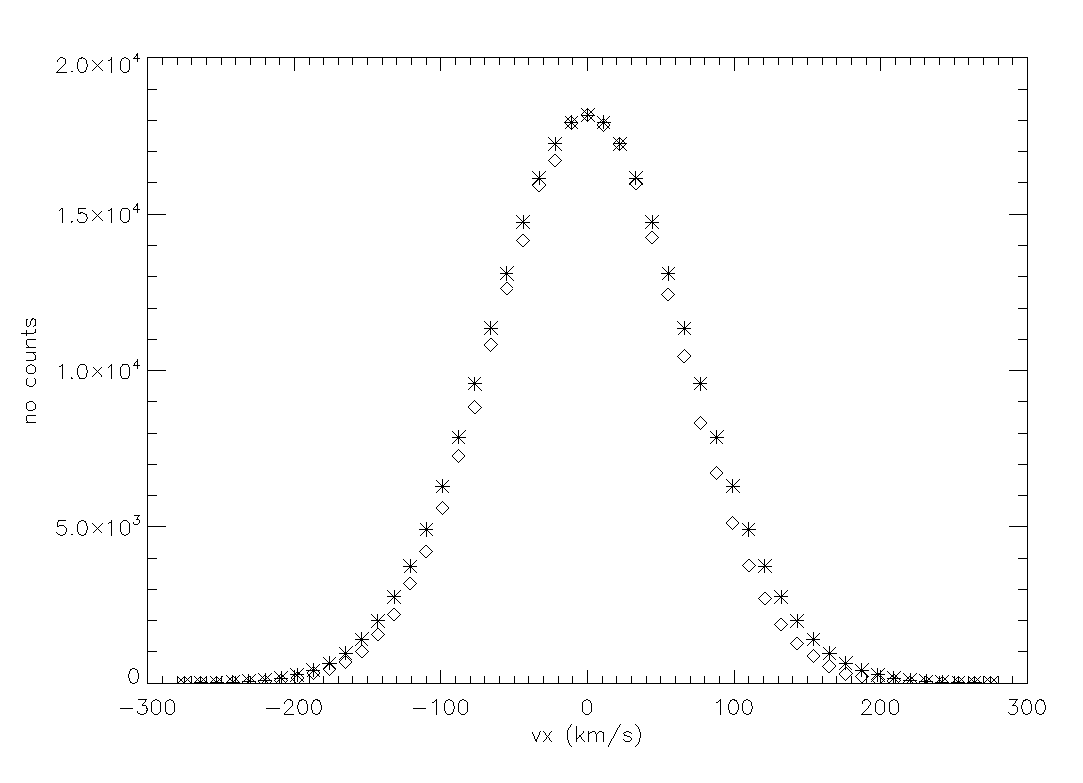
\includegraphics[width=0.49\columnwidth]{./full/gadget/vel/vx_h_hist_0000_z_}
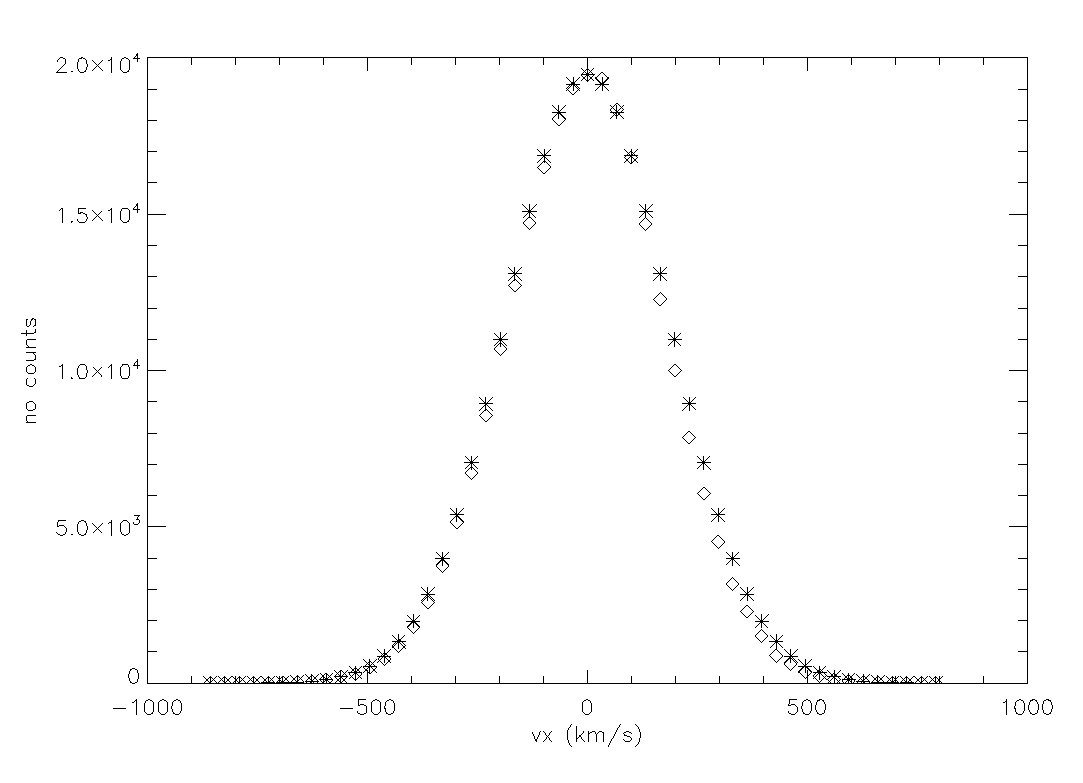
\includegraphics[width=0.49\columnwidth]{./full/gadget/vel/vx_h_hist_000_z_}
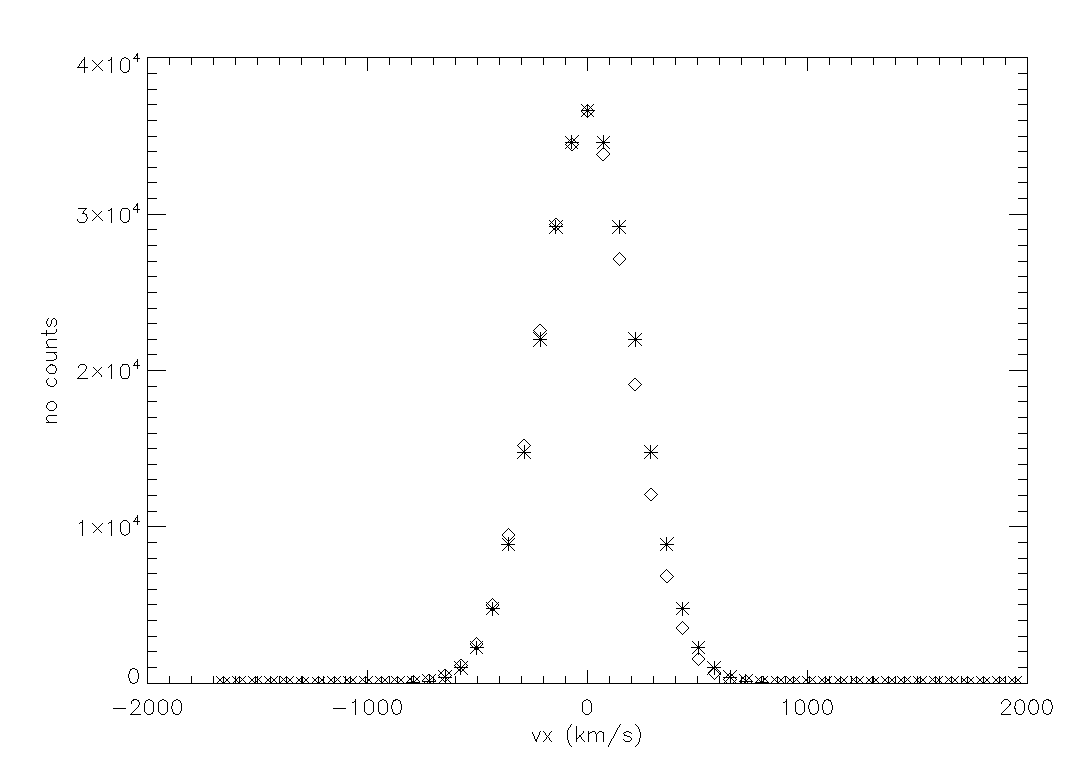
\includegraphics[width=0.49\columnwidth]{./full/gadget/vel/vx_h_hist_001_z_}
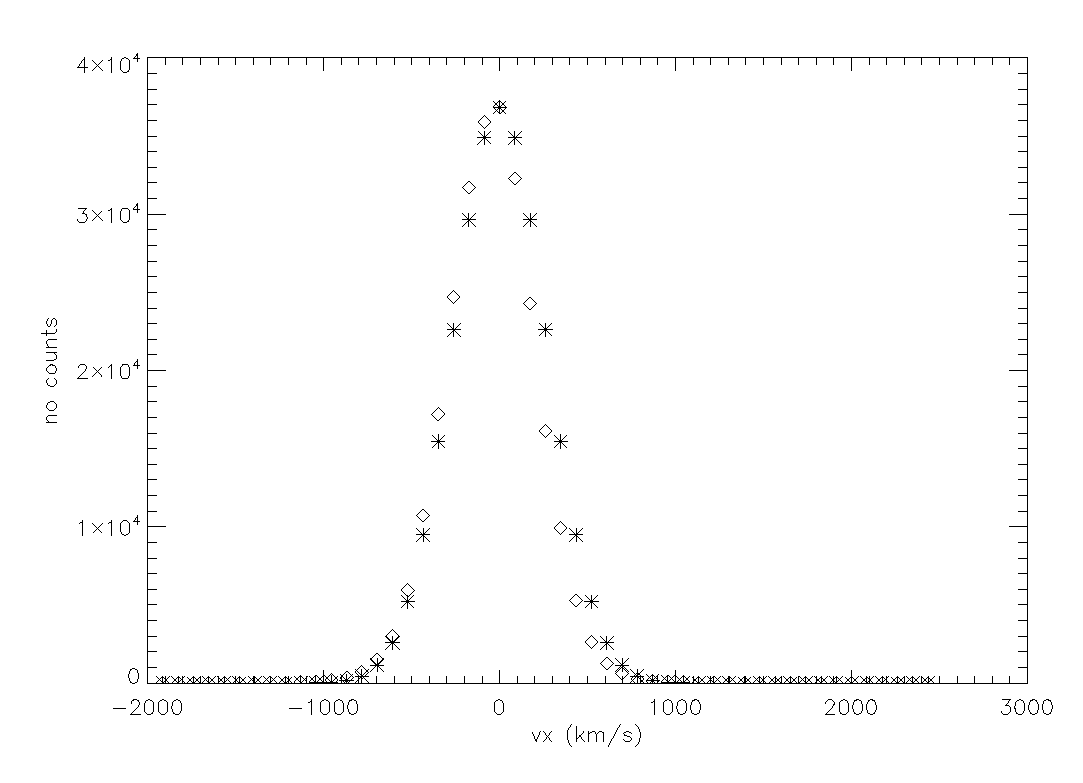
\includegraphics[width=0.49\columnwidth]{./full/gadget/vel/vx_h_hist_002_z_}
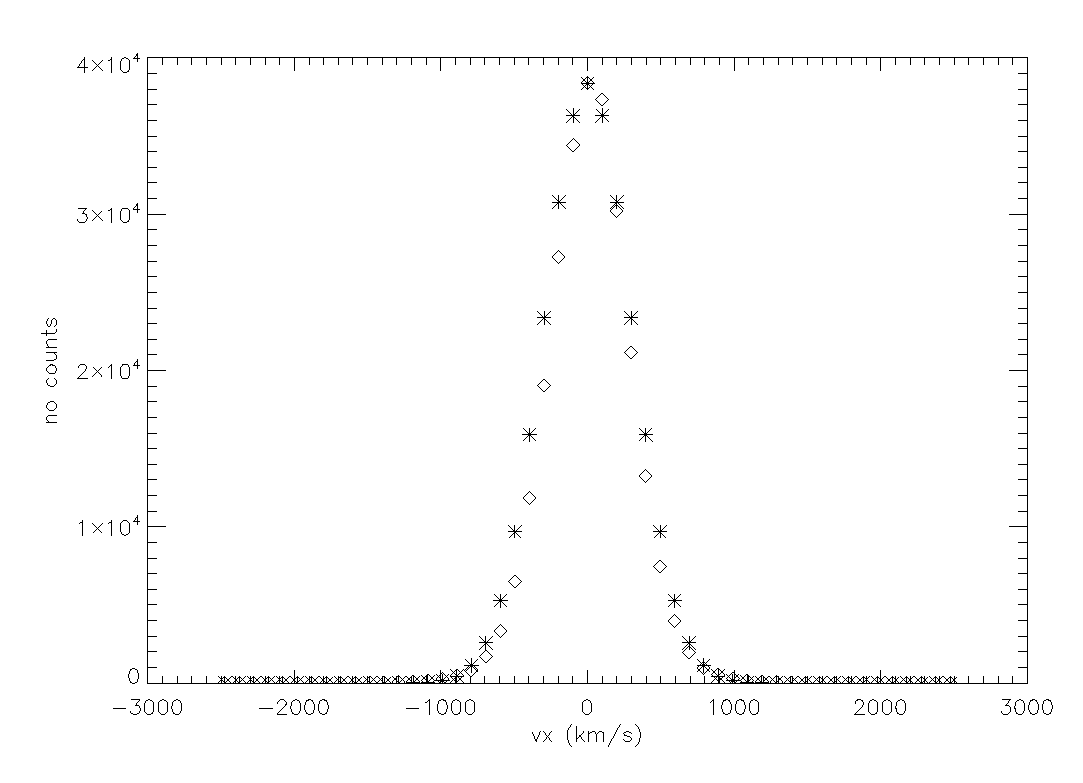
\includegraphics[width=0.49\columnwidth]{./full/gadget/vel/vx_h_hist_003_z_}
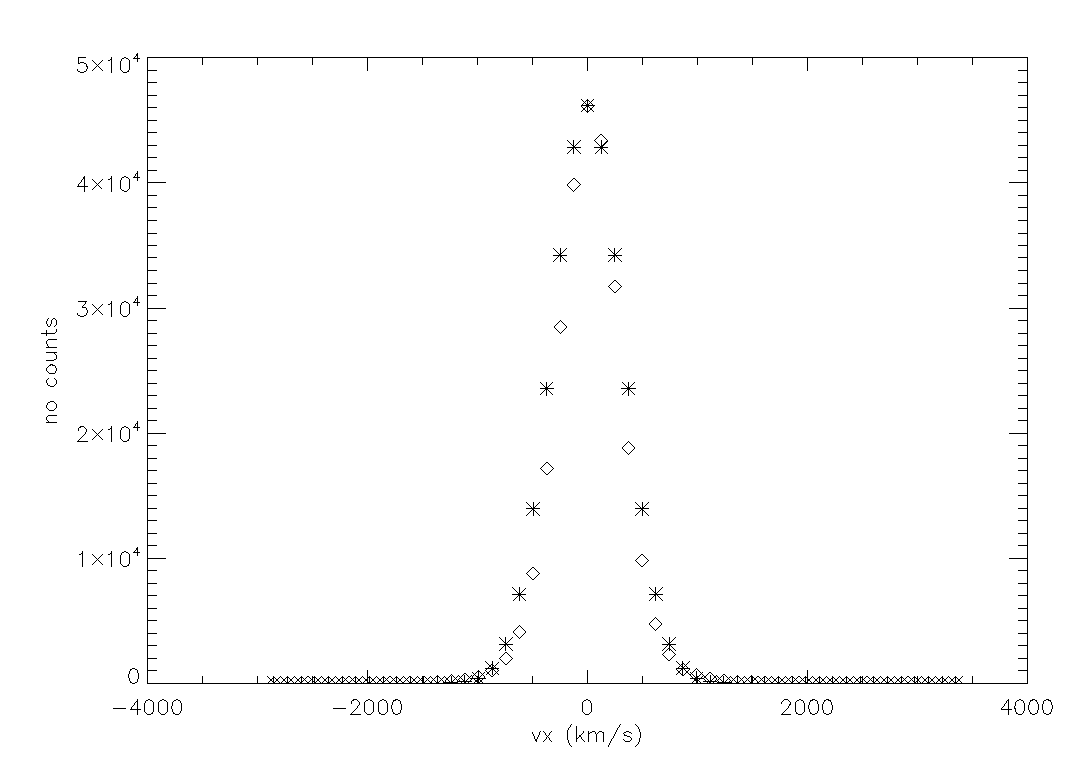
\includegraphics[width=0.49\columnwidth]{./full/gadget/vel/vx_h_hist_004_z_}
   \end{center}
\caption{These plots show a histogram of the $V_x$ component of velocity from the GADGET-2 code. The other velocity components are essentially the same. Overplotted is a theoretical gaussian, shown as asterisks, with the same standard deviation (calculated from the outputted velocity data, shown as diamonds). The times shown are at redshifts: $z = 31, 3, 2, 1, 0.5, 0.05$.}
\label{fig.gadvel}
\end{figure}

\begin{figure}[htb]
   \begin{center}
     %\leavevmode

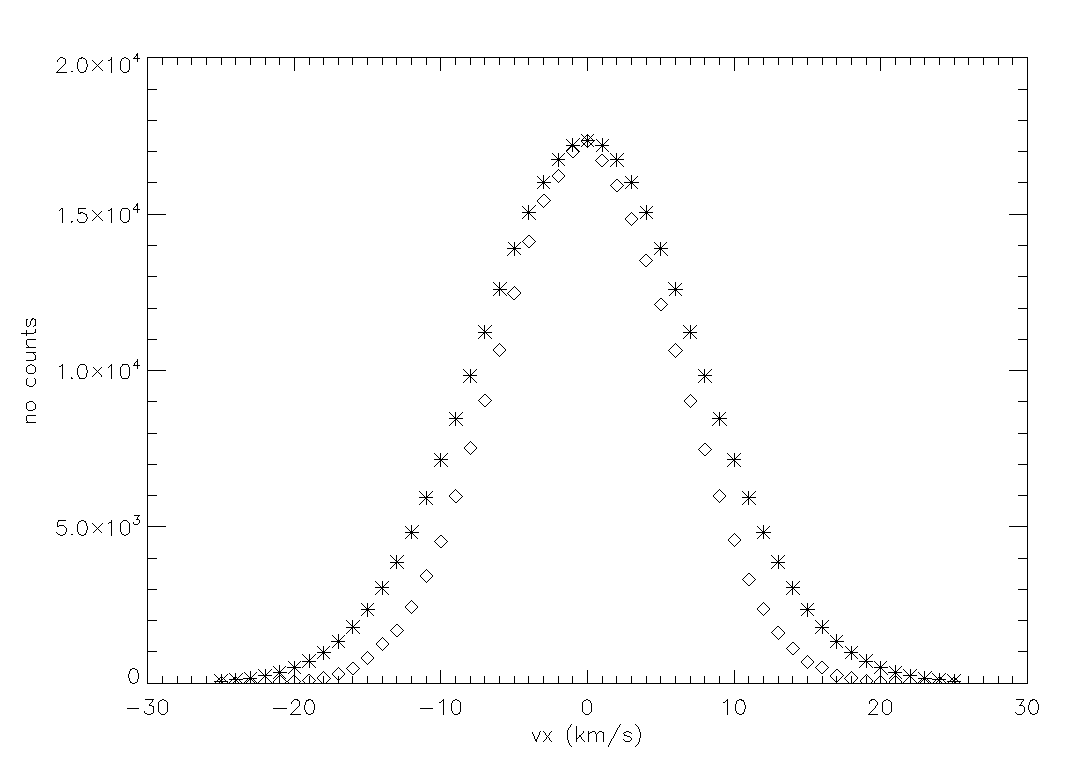
\includegraphics[width=0.49\columnwidth]{./full/wm64/vel/r00000_vxg_hist}
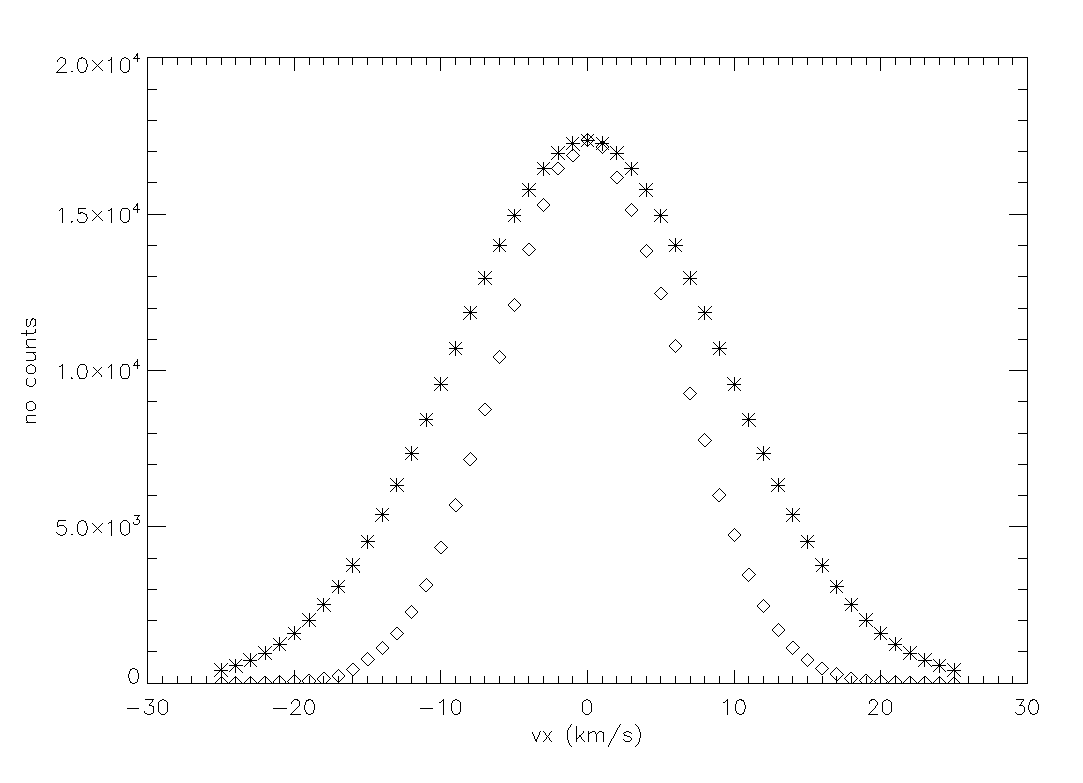
\includegraphics[width=0.49\columnwidth]{./full/wm64/vel/r00200_vxg_hist}
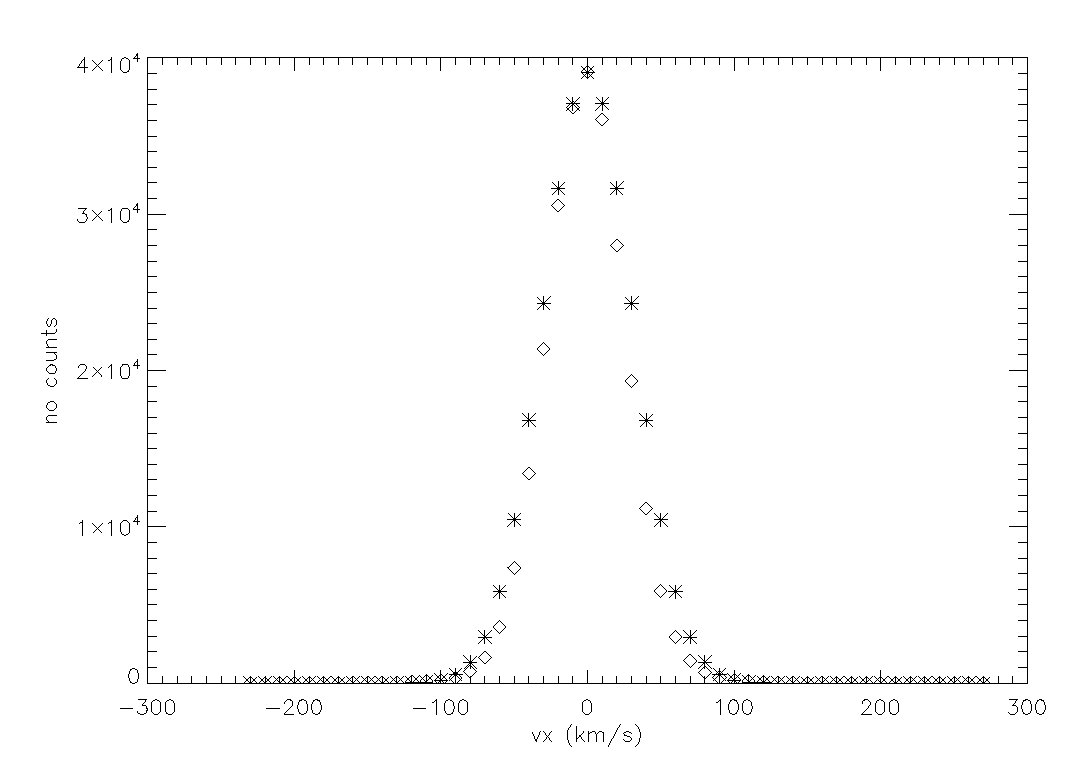
\includegraphics[width=0.49\columnwidth]{./full/wm64/vel/r01000_vxg_hist}
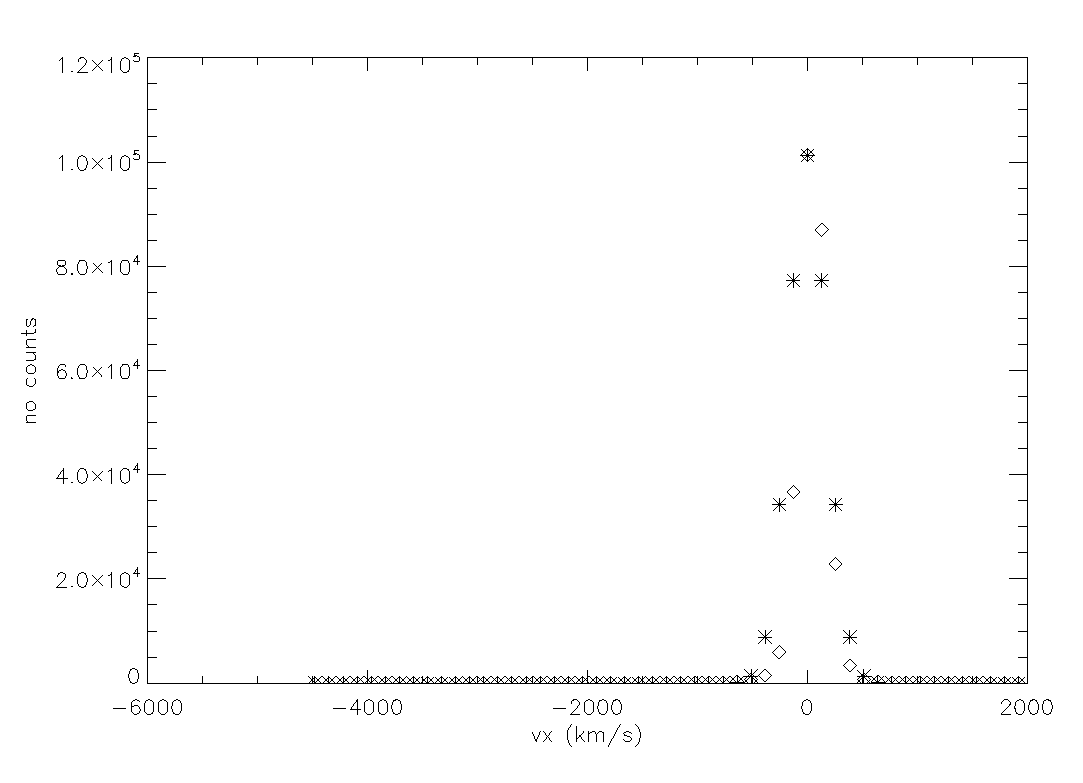
\includegraphics[width=0.49\columnwidth]{./full/wm64/vel/r02000_vxg_hist}
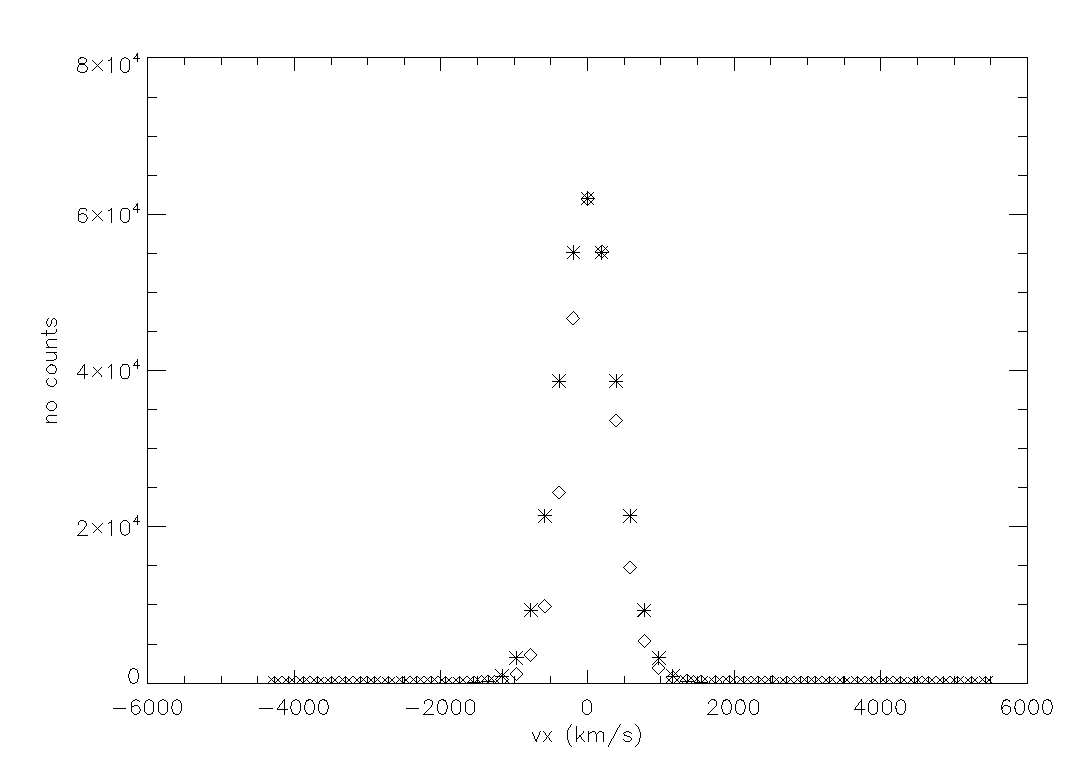
\includegraphics[width=0.49\columnwidth]{./full/wm64/vel/r03000_vxg_hist}
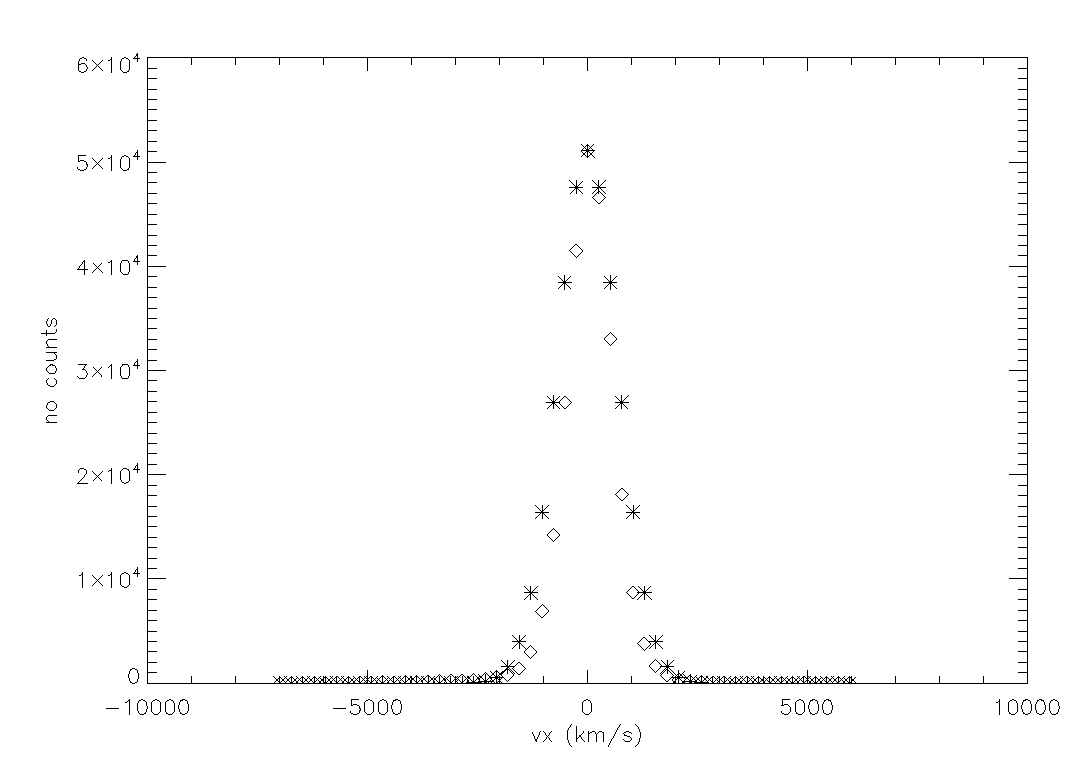
\includegraphics[width=0.49\columnwidth]{./full/wm64/vel/r03500_vxg_hist}

   \end{center}
\caption{These plots show a histogram of the $V_x$ component of velocity from the wave-mechanics code. The other velocity components are essentially the same. Overplotted is a theoretical gaussian, shown as asterisks, with the same standard deviation (calculated from the outputted velocity data, shown as diamonds). As before, the histograms are at times of $t = 0, 200, 1000,$ $2000, 3000, 3500$ ($a = 0.03125,0.038,$ $0.085,0.23, 0.63, 1.03$)}
\label{fig.whvel}
\end{figure}

\begin{figure}[htb]
   \begin{center}
     %\leavevmode

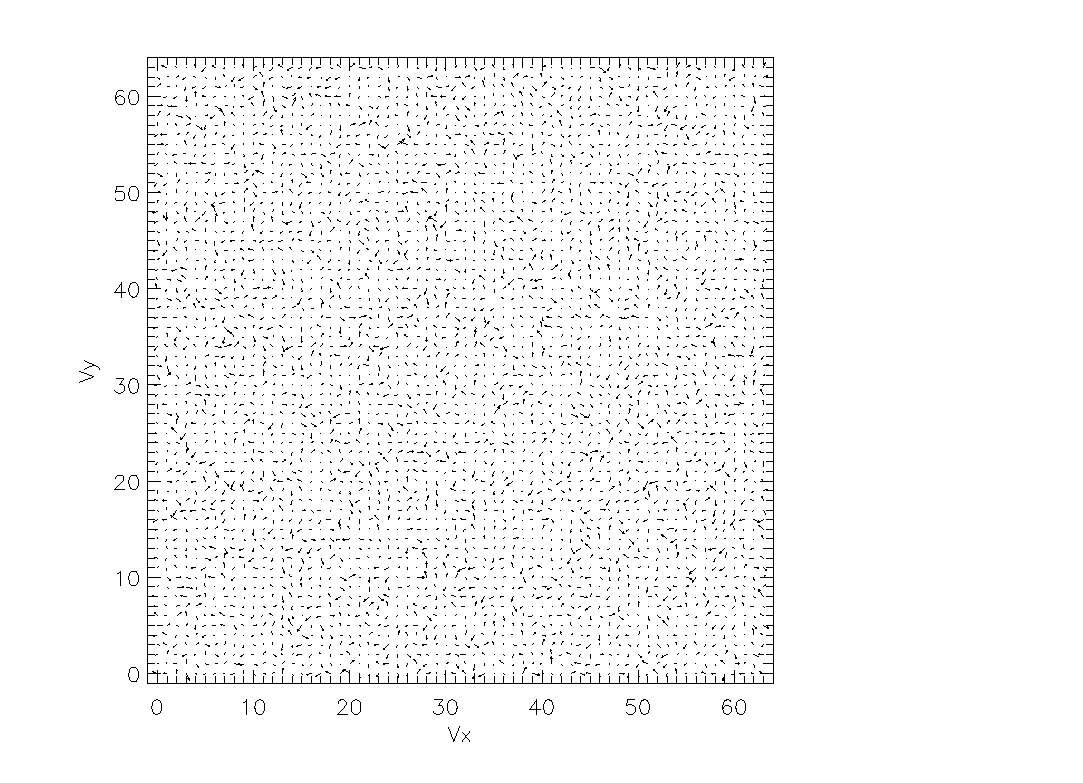
\includegraphics[width=0.49\columnwidth]{./full/wm64/vel/r00000_vel_xy_field}
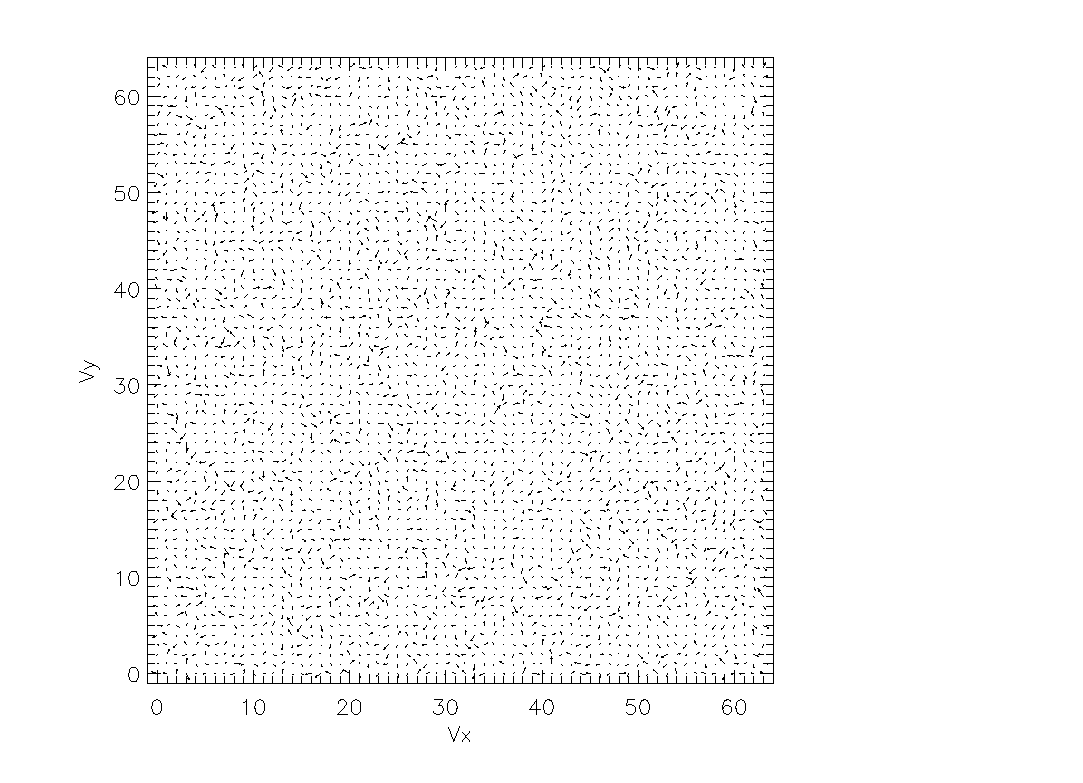
\includegraphics[width=0.49\columnwidth]{./full/wm64/vel/r00200_vel_xy_field}
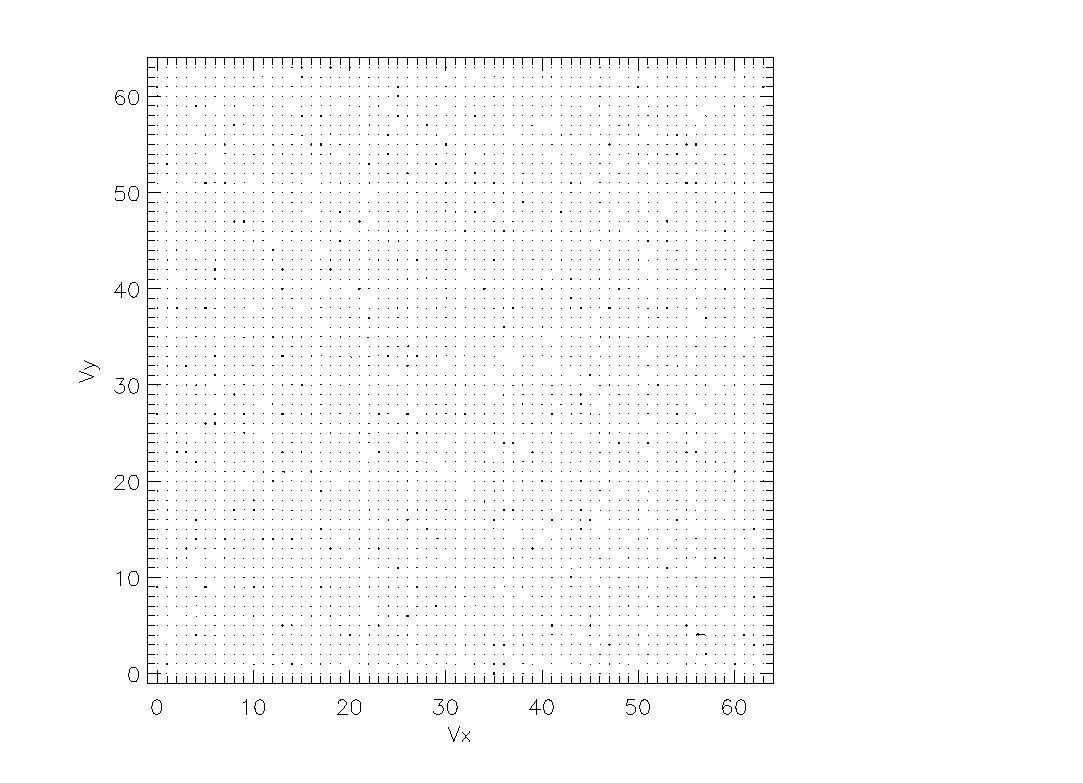
\includegraphics[width=0.49\columnwidth]{./full/wm64/vel/r01000_vel_xy_field}
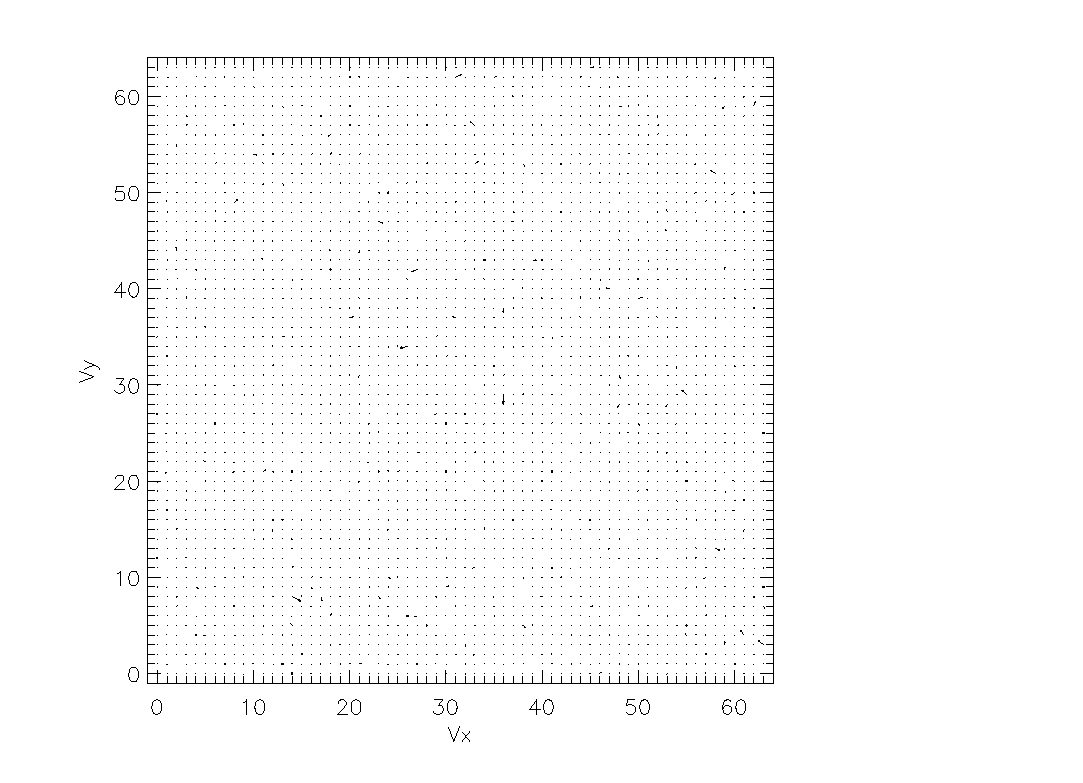
\includegraphics[width=0.49\columnwidth]{./full/wm64/vel/r02000_vel_xy_field}
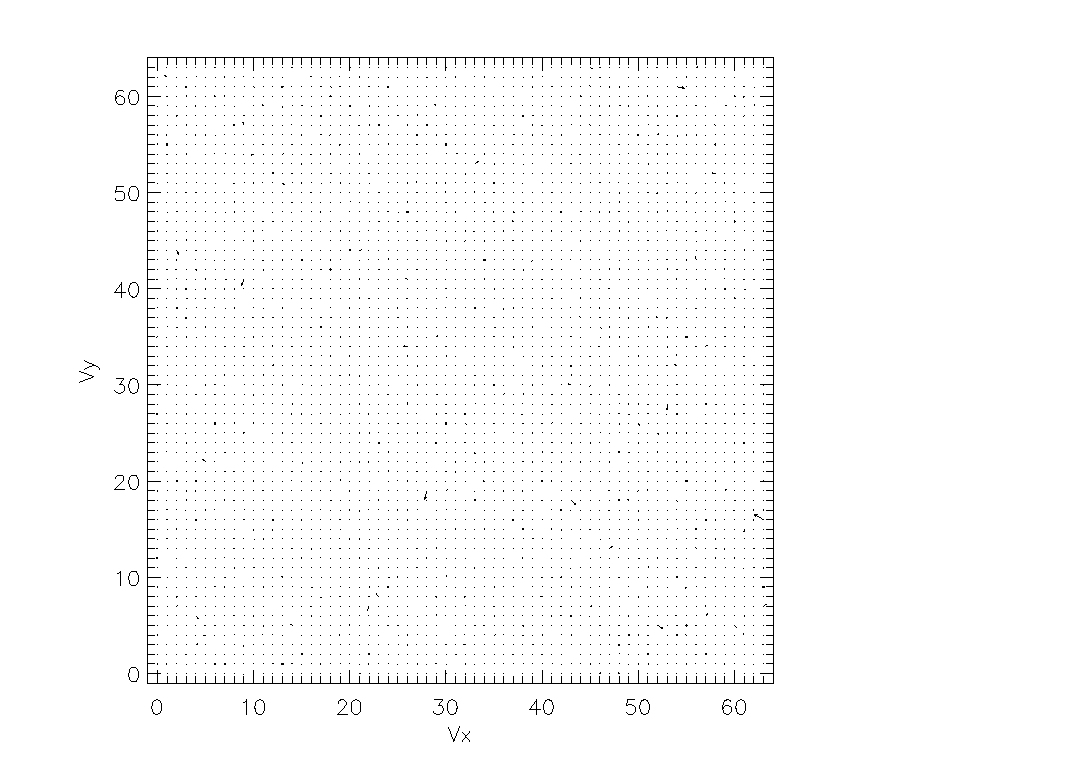
\includegraphics[width=0.49\columnwidth]{./full/wm64/vel/r03000_vel_xy_field}
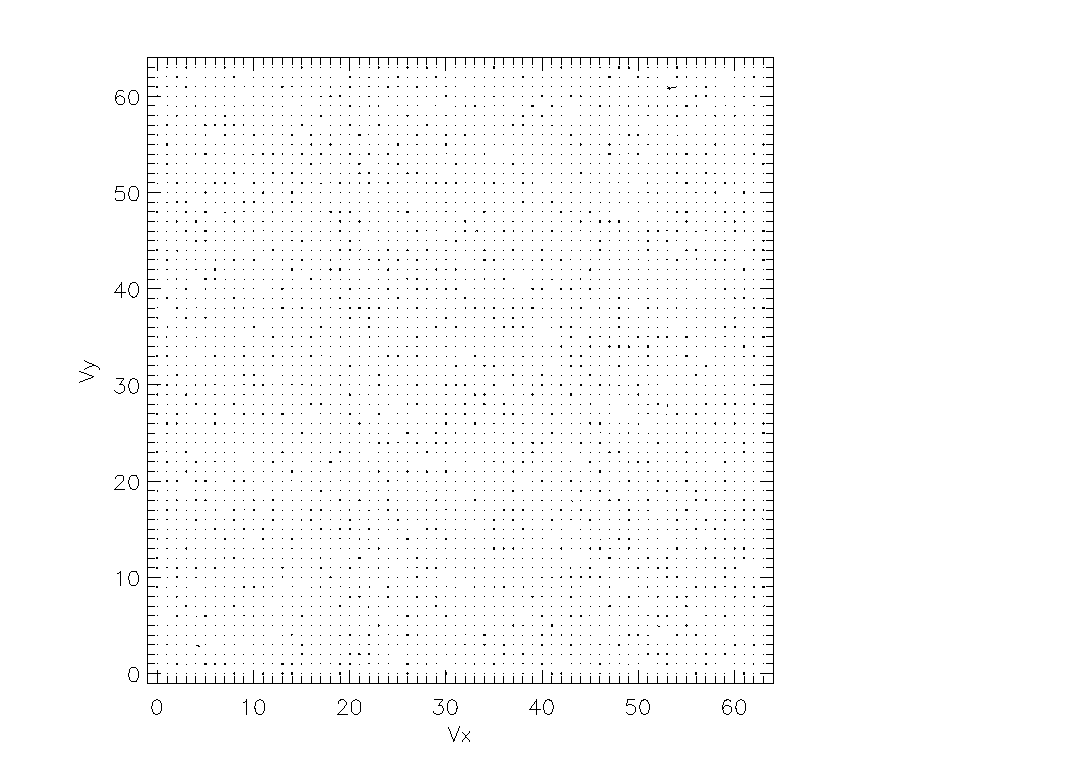
\includegraphics[width=0.49\columnwidth]{./full/wm64/vel/r03500_vel_xy_field}

   \end{center}
\caption{This figure shows quiver plots of the $x,y$ components of velocity from the wave-mechanics code. The velocities are of roughly equal magnitude at early times but this is not true of the later plots. The outputs correspond to the same x,y slice of the data as seen in the previous wave-mechanics plots and at the same times: $t = 0, 200, 1000,$ $2000, 3000, 3500$.}
\label{fig.wmvel}
\end{figure}

\paragraph{Vorticity}
In section \ref{vort} we discussed how to identify possible regions of vorticity, this proved fruitful when analysing the results from the 3D FPA code as seen in section \ref{ch4vort}. In figure \ref{fig.wmvort} the plots show $\mathcal{I}(\psi) \;{\rm vs}\; \mathcal{R}(\psi)$; we suggested that analysing the patterns of these graphs will help to find areas of vorticity and for providing another check of robustness. The first plot shows a ring with an isotropic distribution which implies that both density and velocity are isotropic, this is what we expect from the initial conditions generator supplied by GADGET-2. It also shows that our construction of the wavefunction is consistent with the initial conditions generator.

The results from the full S-P simulation do not seem to show any signs of vorticity, the wavefunction does not appear to get close enough to zero (min$[\psi_{final} \sim 10]$) to become singular. While the lack of vorticity agrees with the standard theory of cosmology, it is not obvious that singularities are prohibited in our formalism. These singularities were shown in the results of the FPA but there is no good reason for their omission in the results of the full S-P system. Given sufficiently enough time to investigate this phenomena I would try running the simulations for longer to see if they will ever produce a singularity in the wavefunction and hence produce an undefined velocity.

\begin{figure}[htb]
   \begin{center}
     %\leavevmode

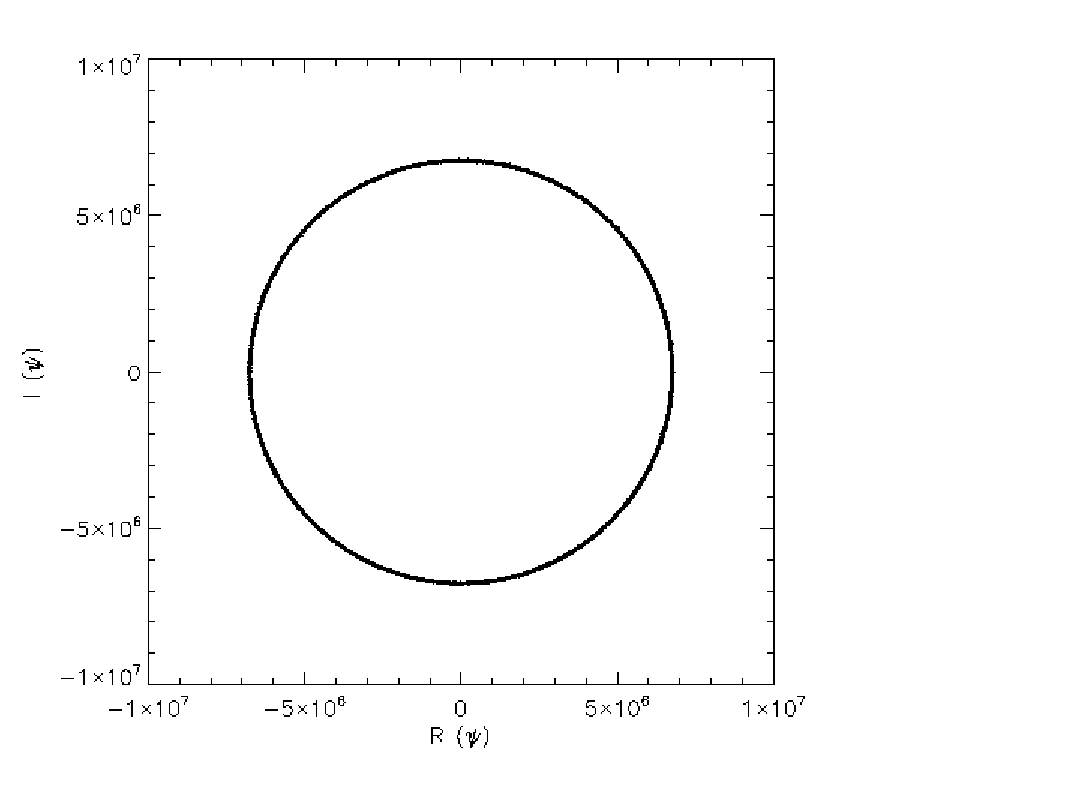
\includegraphics[width=0.49\columnwidth]{./full/wm64/vort/r00000_psi-psi}
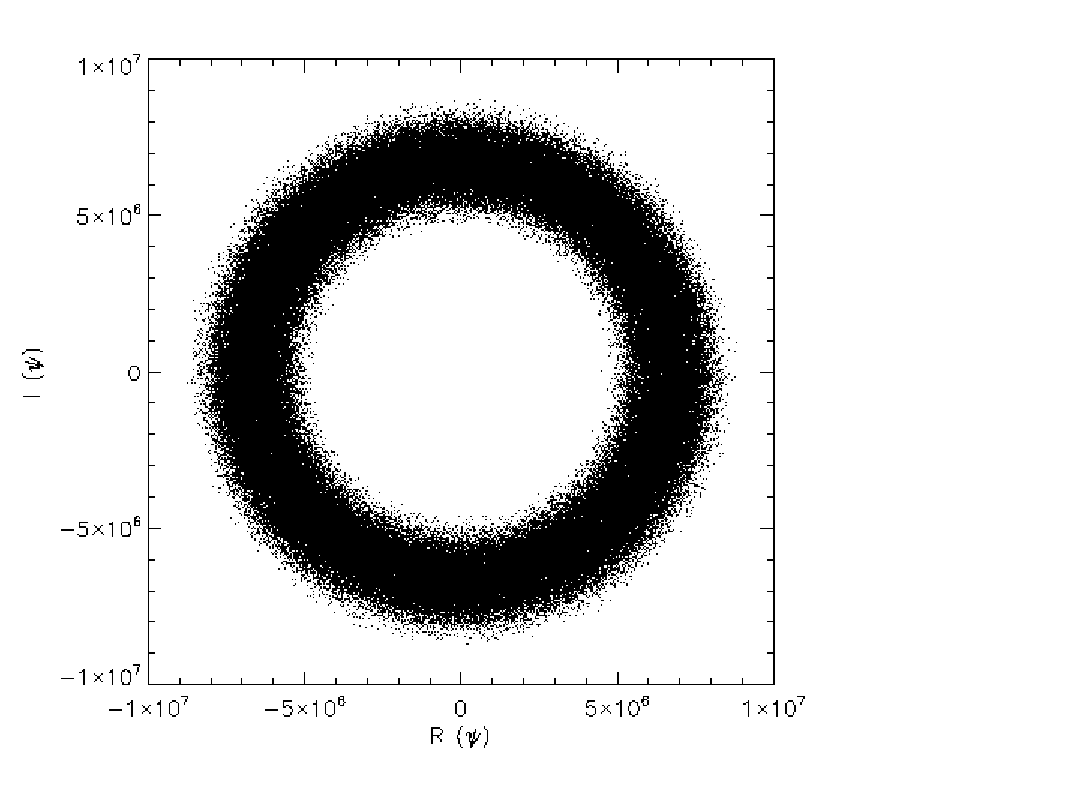
\includegraphics[width=0.49\columnwidth]{./full/wm64/vort/r00200_psi-psi}
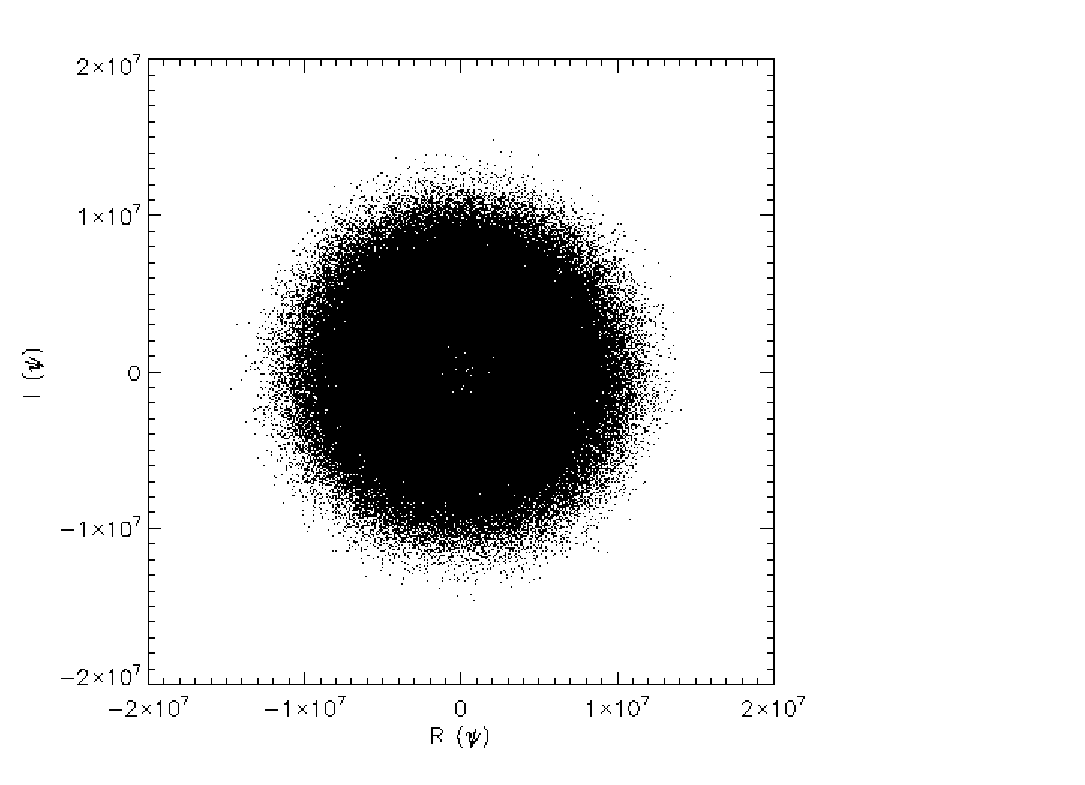
\includegraphics[width=0.49\columnwidth]{./full/wm64/vort/r01000_psi-psi}
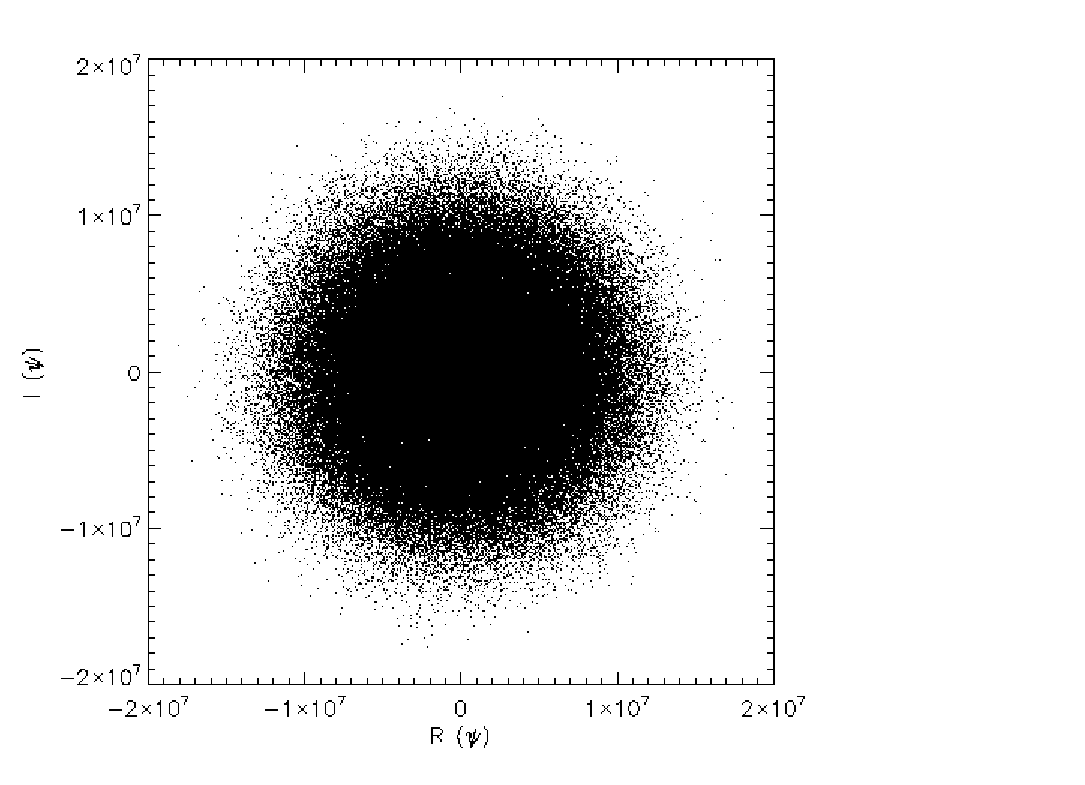
\includegraphics[width=0.49\columnwidth]{./full/wm64/vort/r02000_psi-psi}
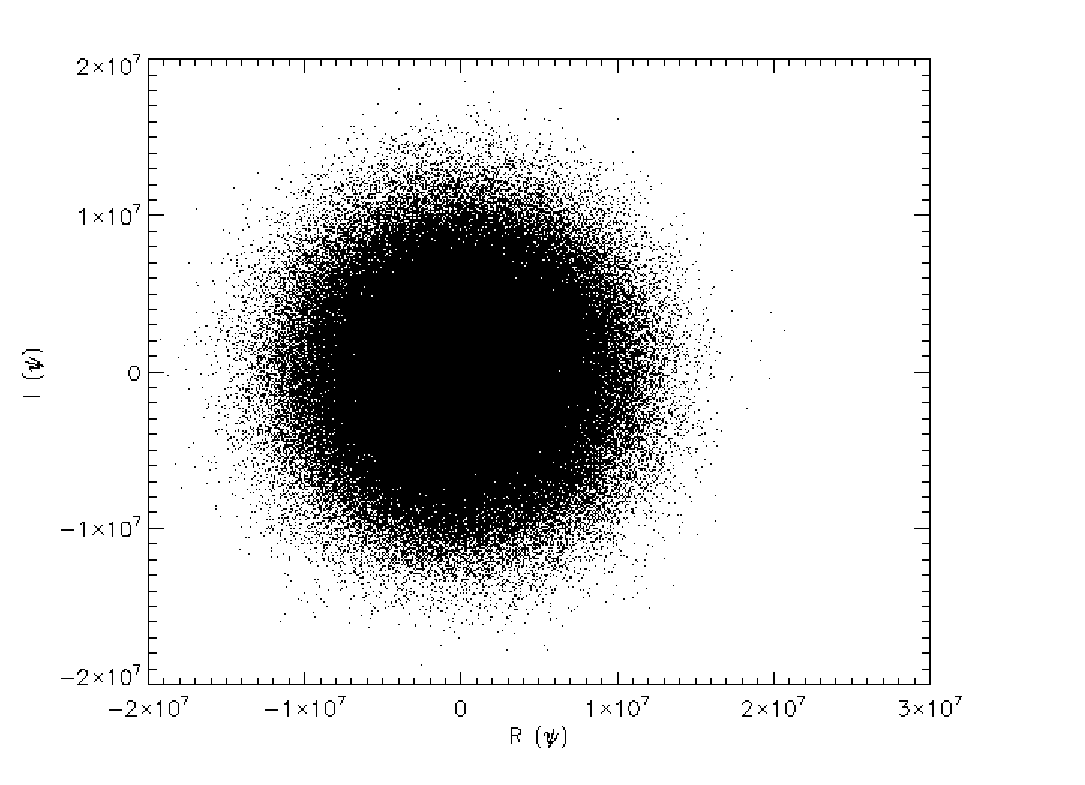
\includegraphics[width=0.49\columnwidth]{./full/wm64/vort/r03000_psi-psi}
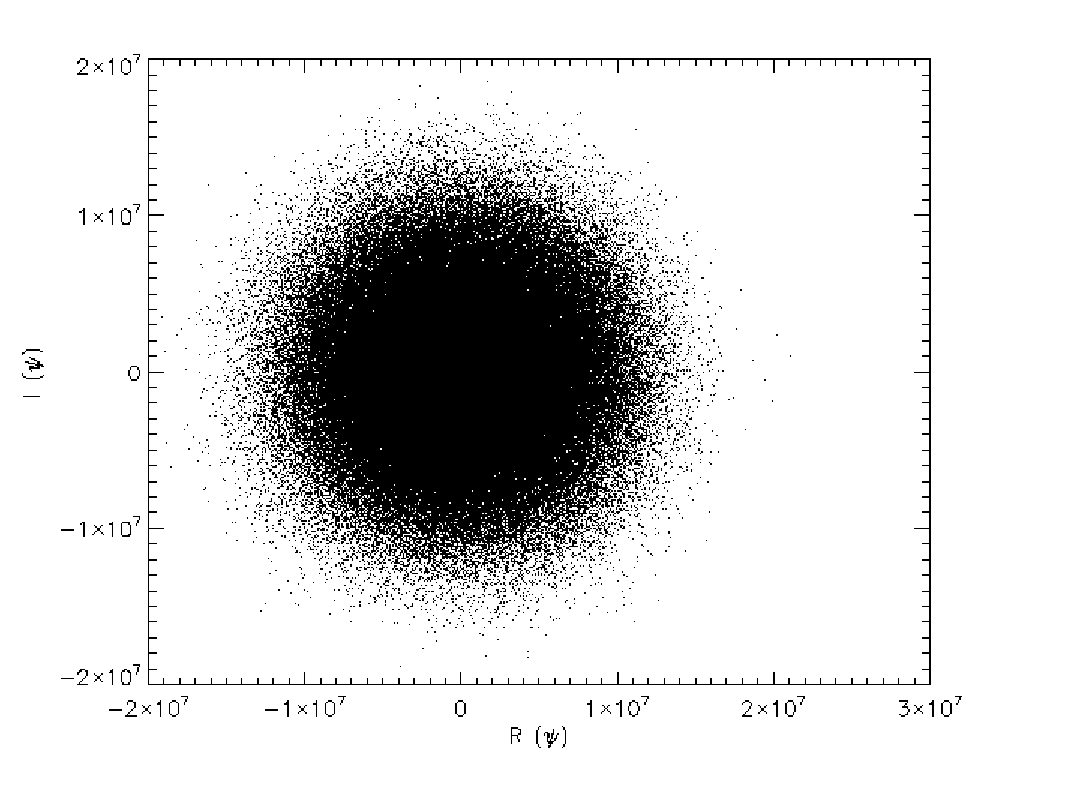
\includegraphics[width=0.49\columnwidth]{./full/wm64/vort/r03500_psi-psi}

   \end{center}
\caption{The plots show $\mathcal{I}(\psi) \;{\rm vs}\; \mathcal{R}(\psi)$. The first plot shows a ring with an isotropic distribution, however the radius is not unity as it was in the FPA, as expected from the initial conditions generator. The smearing out of this ring is indicative that the wavefunction is evolving and hence the over-densities are spread further from the mean. The outputs are at the same times, $t = 0, 200, 1000,$ $2000, 3000, 3500$.}
\label{fig.wmvort}
\end{figure}

\subsection{Known issues and limitations}
\label{known_issues}
Two significant unresolved issues remain in the full S-P code and should be clearly stated:

\begin{enumerate}
\item \textbf{Velocity discrepancy with GADGET.} The velocity distributions from the wave-mechanics code are systematically wider than those from GADGET, even at the initial conditions. This is a major limitation, not a minor calibration issue. The most likely source is the construction of the initial wavefunction using the gravitational potential $\Phi_g$ rather than the velocity potential $\varphi_v$; while these are approximately equal in the linear regime, any residual difference is amplified by the gradient operation. The GADGET velocity scaling ($v_{\rm real} = \sqrt{a}\, v_{\rm code}$) should also be independently verified.

\item \textbf{Spurious growing bulk flow.} The mean velocity drifts systematically over the course of the simulation (from $\sim -4$ to $\sim -165$ km/s in $V_x$), indicating a net bulk motion that should not exist in a periodic, homogeneous simulation. This drift is present in all three velocity components and grows monotonically. The cause is unknown; possible sources include an asymmetry in the discrete Laplacian, a subtle error in the periodic boundary implementation, or accumulation of floating-point errors in the splitting scheme. This issue must be resolved before the code can be used for quantitative velocity-dependent statistics.
\end{enumerate}

\noindent These issues do not invalidate the density results or the conservation properties demonstrated above, but they do mean that velocity-dependent outputs from the code should be treated with caution.

\section{Summary}
This chapter has shown how to implement a wave-mechanics code for Large Scale Structure that satisfies our five original requirements: 3D coordinates, self-consistent gravity, expanding coordinates, periodic boundaries, mass conserving. The use of the full Schr\"odinger-Poisson equations goes beyond the FPA model of Short. That is to say that we have extended the original paper of Widrow \& Kaiser; which includes a generalization of their Schr\"odinger equation to allow for more cosmological models.

The most similar work to what we have done is the full 3D code from the team in Taiwan. Unfortunately, their publication does not provide enough details to make a full comparison with their technique. There are some open questions about their work that are worth addressing: does it conserve mass and momentum? Does it properly implement periodic boundaries? I suspect that the latter is true because it is a necessary requirement of a cosmological code. I'm less sure of the answer to the former question as they do not address the issue and they may regard it as a less important concern. A key strength of our work is that we have shown that our method conserves mass and momentum.

We have provided a clear roadmap for any reader that would like to create their own wave-mechanics code in order to reproduce our results or to be used for their own purposes. All the necessary mathematics has been provided and clear explanations have elucidated why each piece of the code is necessary and how these pieces fit together. It is clear from the works of Watanabe that the Suzuki splitting operators should be used for any simulation of higher dimension than one. Fortunately, they can be implemented with the Goldberg scheme as suggested by Widrow \& Kaiser (essentially the same as Watanabe's approach). Furthermore, we have shown that the use of splitting operators and the Goldberg scheme can be consistently implemented with periodic boundary conditions and coordinate expansion.

We believe that the implementation of periodic boundaries is completely new as previous publications have not mentioned such considerations. As such, we can confidently state that this is the first illustration of such a method. Also new to this thesis is the generalization of Schr\"odinger equation to describe more general cosmological models.

Proof of multi-streaming (described in section \ref{hydro}), or shell crossing, is clearly shown in the results from the 3D code as seen in section \ref{twobody}. The tophat results show the inclusion of gravity and of a simple cosmologically-based scenario. Such results combined with the conservation of key quantities (mass and momentum) suggest that our final results in section \ref{cos_sim} may be correct but require further investigation. That the whole simulation shares a single wavefunction allows for the possibility of interference, despite our intention to suppress these effects it is still possible that interference is present in our final results (given the apparent messiness of our 3D cosmological results).

A key concern to address is why the density outputs from the wave-mechanics code are not closer to that of GADGET-2. We expect the results from wave-mechanics to differ from GADGET-2 but it appears that the variation in densities and the patterns produced by wave-mechanics are far greater than expected. As shown in Chapter \ref{ch_4}, the densities from wave-mechanics provided reasonable correlation coefficients with the densities from Hydra. Mass is conserved and the distributions are not completely random; they show a clear pattern of evolution that is different from what we expected but not necessarily wrong. Unfortunately we cannot conclude whether our results are completely correct within the wave-mechanics framework. That is to say that we suspect the wave-mechanics framework is robust and can be correctly applied to LSS simulations but we have not been able to prove that beyond all doubts in this thesis. 

The biggest problem of the wave-mechanics code is the off-centre velocity distribution which suggests a net bulk motion. From theory, the net motion of the Universe should be zero (ignoring suggestions that the Universe might be rotating as a whole). The velocity scaling also appears to be wrong and will need to be addressed in future research.

